\documentclass[newtx, it, fancy, 11pt, hang]{mybook}

\title{Computer and Network Security}
\subtitle{Ingegneria dell'Automazione}
\institute{Università di Roma Tor Vergata}
\date{\today}
\cover{logo.png}
\logo{logouni.png}

\begin{document}

\maketitle

\frontmatter
\tableofcontents

\mainmatter
\chapter{Introduzione sulla Crittografia}
\section{Cifratura}
Quando vogliamo cifrare il contenuto di un messaggio in chiaro (\emph{plaintext}) abbiamo bisogno di un cifratore che sia in grado di trasformare il messaggio in un messaggio cifrato (\emph{cyphertext}) e un secondo cifratore in grado di decriptare il messaggio in modo tale da ottenere nuovamente un testo leggibile dal ricevitore. 
\begin{figure}[h]
    \centering
    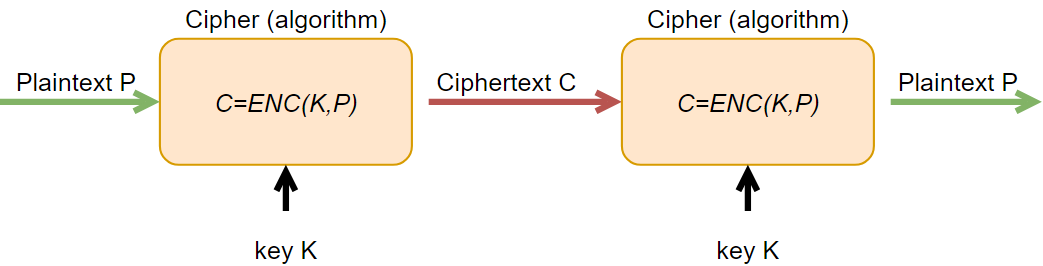
\includegraphics[width=\textwidth]{image/enc_exemple.png}
    \caption{Schema di Crittografia Standard}
    \label{fig:enc_exemple}
\end{figure}\\
La cifratura è una tecnica che serve \textbf{proteggere la confidenzialità dei dati} trasformandoli in qualcosa di incomprensibile ad un interprete generico. Come indicato nella \cref{fig:enc_exemple}, \textbf{la trasformazione} messa in atto da un cifratore \textbf{deve essere reversibile}, in modo tale che il destinatario del messaggio cifrato sappia ritrasformare il testo cifrato per poterlo leggere. Al fine di fare ciò, entrambe le parti devono conoscere due fattori:
\begin{enumerate}
    \item \textbf{Chiave:} la chiave è l'informazione che \textbf{deve} essere segreta e condivisa solo ed esclusivamente tra il mittente e il destinatario. Può essere di tipo \textbf{simmetrico} se viene usata la stessa chiave per cifrare e decifrare il messaggio, \textbf{asimmetrica} altrimenti. 
    \item \textbf{Algoritmo di Cifratura:} il meccanismo che applica la trasformazione al plaintext sulla base della chiave che viene segreta. Tipicamente gli algoritmi sono pubblici e standardizzati. 
\end{enumerate}
\subsection{Tecniche di Cifratura}
\begin{proposition}[Substitution Cypher]
Tecnica di cifratura che opera per sostituzione di lettere secondo un preciso schema (es: $A\rightarrow{B}$).
\end{proposition}
Il problema di sostituire secondo uno schema, detto dizionario, è che con un'analisi più o meno attenta (\emph{ad esempio analizzando la frequenza di ripetizione delle lettere}) è possibile dedurre lo schema di sostituzione e ricostruire il messaggio originale senza la chiave che era stata usata per cifrarlo. 
\begin{proposition}[Vernam Cypher]\label{prop:vernam}
Tecnica di cifratura che, dato un messaggio di lunghezza $L$, usa una chiave \textbf{randomica}\footnotemark di lunghezza $\hat{L}=L$ che vengono unite tramite $\oplus$ (xor) per generare il messaggio cifrato. Infine, sempre tramite $\oplus$, il messaggio viene decifrato usando la stessa chiave.
\footnotetext{La chiave deve essere generata in modo \textbf{truly random} ossia veramente casuale. Impossibile da fare tramite funzioni semplici, che generano sequenze di numeri pseudo-random.}
\end{proposition}
\begin{property}[XOR]
Ricordiamo che: $A\oplus{0} = A,\,A\oplus{1} = A',\, A\oplus{A'} = 1$.
\end{property}
Il vernam cypher è considerato il meccanismo di cifratura \emph{perfetto} in quanto se le ipotesi su cui si basa sono soddisfatto, il messaggio ottenuto in uscita è indecifrabile senza l'opportuna chiave. Tuttavia non è realizzabile, per i seguenti motivi:
\begin{enumerate}
    \item \textbf{Una chiave per ogni messaggio:} La robustezza del cifratore si basa sull'utilizzo di una chiave, completamente randomica, per ogni messaggio che viene inviato. Supponiamo di usare la stessa chiave $K$ per due messaggi cifrati $C_1$ e $C_2$ e facciamone lo $\oplus$:
    \begin{center}
    \vspace{-25pt}
        \begin{equation*}
            C_1\oplus{C_2}=(M_1\oplus{K})\oplus(M_2\oplus{K})=M_1\oplus{M_2}
        \end{equation*}
    \end{center}
    In questo modo abbiamo dedotto l contenuto del messaggio cifrato senza neanche sapere la chiave. Noto questo, tramite un \emph{Chosen Plaintext Attack} (attacco tramite invio di messaggi scelti), potremmo dedurre anche la chiave. 
    \item \textbf{Ogni chiave deve essere lunga quanto il messaggio:} Non un reale problema computazionale. Per rendere la chiave lunga quanto il messaggio, possiamo ripetere i caratteri della chiave se sono troppo pochi o usare metodi più sofisticati. Tuttavia scomodo dal punto di vista della scalabilità. Per $1GB$ di messaggio dovremmo disporre una chiave di $1GB$.
    \item \textbf{La chiave deve essere truly random:} impossibile da generare con funzioni di libreria o tecniche particolari, in quanto il numero casuale è definito da un algoritmo e, pertanto, generabile da terzi.
\end{enumerate}
\begin{corollary}[Lo scopo della crittografia]
Quando criptiamo un messaggio dobbiamo ragionare in ottica di \textbf{mettersi in sicurezza da una minaccia specifica}, piuttosto che da un pericolo in generale.
\end{corollary}\pagebreak
\section{Confidentiality, Integrity, Availability}
I principi alla base della cifratura e della crittografia sono i seguenti:
\begin{definition}[Confidentiality]\label{def:confidentiality}
Misura adottata per evitare che le informazioni sensibili arrivino alle persone sbagliate, assicurando che solo chi sia autorizzato possa accedervi.
\end{definition}
\begin{definition}[Integrity]\label{def:integrity}
Con il concetto di integrità si vuole specificare che, durante la trasmissione di un un messaggio, questo arrivi a destinazione \textbf{integro e senza che qualcuno possa alterarne il valore}
\end{definition}
\begin{definition}[Authenticated Encryption with Associated Data]\label{def:aead}
Un sistema in grado di garantire sia integrità che confidenzialità è detto di tipo AEAD.
\end{definition}
\begin{definition}[Availability]
Mantiene aggiornato e bug-free il software che veicola lo scambio del messaggio.
\end{definition}
Difatti, il modello di cifratura utilizzato fino ad ora non copre i casi in cui una minaccia intenta ad effettuare un attacco di tipo \emph{Man in the Middle (MITM)} riesca a modificare un bit o più del messaggio, modificandone il contenuto e passando inosservato. Possiamo dire che:
\begin{proposition}
Una cifratura mantiene un'\textbf{elevata confidenzialità} ma una \textbf{scarsa integrità}.
\end{proposition}
\begin{example}[ RFID:]
E' un sistema composto, solitamente, da un \emph{TAG} e un \emph{READER} (per esempio la carta e il pos). Per il funzionamento è necessario che tra i due oggetti ci sia una mutua autenticazione in quanto sia il \emph{TAG} che il \emph{READER} potrebbero non essere autentici.\\
Tipicamente un \emph{TAG} è composto da:
\begin{itemize}
    \item Un segreto, statico, $S$
    \item Una chiave, temporanea, $K$
\end{itemize}
Il messaggio contenente il segreto viene cifrato tramite $\oplus$ con la chiave associata all'utente.\\
Il \emph{READER} invece detiene un database con le chiavi degli utenti a cui fare riferimento.\\
Quando il \emph{TAG} viene a contatto con il \emph{READER}, quest'ultimo sarà in grado di decifrare il messaggio qualora fosse genuino, trovando un riscontro con qualche entry del database.\\
In questo sistema, ogni chiave è generata \textbf{pseudo-randomicamente} a partire dalla chiave precedente. Una volta ottenuto il segreto, il \emph{READER} associa una nuova chiave temporanea al \emph{TAG} in questione, aggiornando il suo database.\\\pagebreak
\begin{remark}
In un \emph{RFID} il segreto viene criptato usando una \emph{pseudo-random key}.
\end{remark}
Tale sistema presenta due problemi. Supponiamo che $S$ sia truly random e $K$ pseudo-random, allora:
\begin{itemize}
    \item Se $S$ è il plain-text, andando in \emph{xor} con $K$ \textcolor{red}{\textbf{viola la proprietà 3}} dei cifratori, in quanto la chiave non è truly random.
    \item Se $K$ è il plain-text, $S$ fa da chiave, ma \textcolor{red}{\textbf{viene violata la proprietà 1}}, in quanto la stessa chiave è associata a messaggi differenti.
\end{itemize}
Poiché l'algoritmo pseudo-random per generare la chiave è noto, è possibile dedurre tutte le possibili combinazioni di bit che costituiscono $K$. Pertanto, facendo uno \emph{xor} tra due messaggi consecutivi, è possibile ottenere un testo con cui fare \emph{xor} con una delle due chiavi, ottenendo delle combinazioni possibili per il plain-text originale.\\
Dato che $M_1\oplus{M_2}=7$, supponendo che $K_i=3,\,k_{i+1}=4$, confrontando con la mappa delle chiavi pseudo-random è possibile dedurre sia chiave, che messaggi che lo schema con cui vengono generate le chiavi.
\begin{figure}[h]
    \centering
    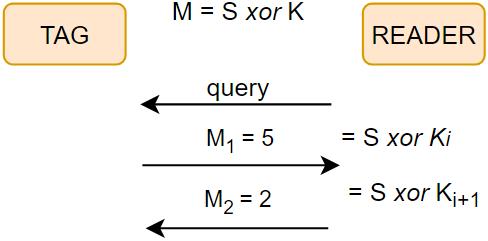
\includegraphics[width=0.6\textwidth]{image/rfid_example.png}
    \caption{Esempio di scambio messaggi in RFID}
    \label{fig:rfid_example}
\end{figure}

\end{example}\pagebreak
\section{Indistinguishability under Chosen Plaintext Attack}
Definire un \emph{"cifratore sicuro"} è generalmente difficile, in quanto una buona definizione deve tenere in considerazione la minaccia rispetto alla quale è considerato sicuro. Tipicamente viene adottata infatti la convenzione \textit{\textbf{Goal-Model}}.\\
Poiché un tipo di attacco è il cosiddetto \textbf{\textit{Chosen Plaintext Attack} (CPA)} una definizione che possiamo dare è che sia di tipo \textbf{IND-CPA}, ovvero, non deve rilasciare informazioni ad un'entità malevola quando questa possa attaccare il sistema sfruttando un plaintext scelto. Facciamo un esempio:
\begin{enumerate}
    \item Supponiamo che un attaccante \textit{A} abbia a disposizione due messaggi $M_0,M_1$ della stessa dimensione, che invia \textbf{in chiaro} ad un utente.
    \item L'utente sceglie randomicamente uno dei due, rispondendo ad \textit{A} con un messaggio cifrato: $C=ENC(K,M_0/M_1)$
    \begin{itemize}
        \item L'attaccante ha il $50\%$ di probabilità di ricevere uno dei due messaggi.
    \end{itemize}
    \item Supponiamo di avere a disposizione un \textbf{Oracolo}, in grado di conoscere \textit{l'associazione \textbf{chiave-testo cifrato}}. L'attaccante invia $M_0,M_1$ all'oracolo, che conoscendo $K$ può rispondere con $C_0=ENC(K,M_0),C_1=ENC(K,M_1)$.
    \item A questo punto l'attaccante confrontando le risposte ricevute, può individuare la chiave con cui viene eseguita la cifratura, con la stessa probabilità dei messaggi spediti all'utente.
\end{enumerate}
\begin{remark}
La chiave rappresenta un fattore fondamentale per garantire la confidenzialità, per questo sarebbe ideale avere a disposizione una chiave diversa ogni volta. In questo modo un attaccante non avrebbe possibilità di capire quale messaggio cifrato corrisponde ai suoi plaintext perché ogni volta riceverebbe un messaggio diverso.
\end{remark}
Le proprietà di un sistema dotato di \textit{"Indistiguishability"} sono:
\begin{itemize}
    \item Un avversario non deve essere in grado di ricavare alcuna informazione su un plain text a partire dal cipher text, anche se egli può avere accesso ad un oracolo.  
    \item L’encryption deve essere randomizzata, poiché uno stesso messaggio deve sempre essere criptato in diversi cipher text, che deve essere indistinguibile da uno randomico. 
    \item Se la sequenza si ripete essa deve essere criptata con una chiave differente
\end{itemize}
\begin{corollary}[XOR e Segretezza]
Dato il funzionamento dell'operatore $\oplus$, se cifriamo una sequenza di bit informativi con una sequenza di bit perfettamente randomica, possiamo dire con certezza che la sequenza generata in uscita sarà ancora casuale al 100\%. La probabilità di indovinare il plaintext a partire da quello cifrato è, a priori, quella di indovinare un numero casuale. Che sarebbe la stessa senza aver visto alcun cipher-text.
\end{corollary}

\chapter{Stream Ciphers}\label{chap:streamcipher}
Sono una categoria di cifratori, tipicamente veloci nell'elaborazione del testo. Un esempio di stream cipher è il \textit{Vernam Cipher}. L'idea di base per uno stream cipher è quella di utilizzare una \textbf{chiave statica} che, unita ad un vettore di bit, permette di ottenere un messaggio cifrato.
\begin{figure}[h]
    \centering
    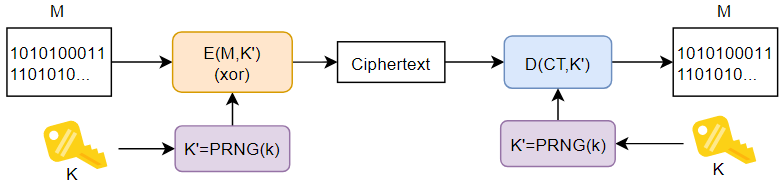
\includegraphics[width=\textwidth]{image/streamcipher.png}
    \caption{Stream Ciphers Scheme}
    \label{fig:stream_ciphers}
\end{figure}\\
In modo tale da rendere uno stream cipher sicuro da un \textit{CPA}, introduciamo il concetto di \textbf{Keystream}. Poiché una caratteristica richiesta per i cifratori era, la necessità di avere una chiave della stessa lunghezza del messaggio che fosse \textit{\textbf{sempre}} nuova, possiamo usare la chiave segreta precedentemente scambiata in qualche modo, come seed per un keystream generato tramite un algoritmo \textit{pseudorandom} che va in $xor$ con il messaggio.\\
\begin{remark}
E' importante non confondere la chiave random del One Time Pad con il keystream generato tramite algoritmo pseudorandom.
\end{remark}
\begin{remark}
L'algoritmo che genera il keystream è ciò che differenzia un cifratore dall'altro. Alcuni esempi sono \textbf{RC4, Salsa20, ChaCha20}.
\end{remark}
\begin{proposition}[Pro e Contro]
\begin{itemize}
    \item [\textcolor{green}{\textbf{PRO:}}]Lo schema in \cref{fig:stream_ciphers} permette di ottenere un testo cifrato in cui se una sotto-sequenza di bit si ripete, ogniuna verrà cifrata \textbf{sempre} in modo diverso.
    \item [\textcolor{red}{\textbf{CONS:}}]Se il messaggio viene cifrato una seconda volta, il testo cifrato sarà comunque \textbf{sempre} uguale a se stesso.
\end{itemize}
\end{proposition}
\section{Gli Initialization Vectors}
Poiché uno stream cipher implica l'utilizzo di una chiave statica e l'algoritmo di pseudo-random è deterministo per definizione, un messaggio verrà cifrato sempre nello stesso modo. Questo significa che perdiamo la proprietà di \textit{IND-CPA}.\\
Gli Initialization Vectors sono dei vettori di numeri generati randomicamente ad ogni nuovo messaggio inviato che permettono di mantenere una \textit{sicurezza semantica}\footnotemark  a patto che \textbf{\textit{non si ripetano MAI}}.
\footnotetext{Un cifratore è \textbf{semantically secure} se è impossibile estrarre informazioni sensibili del plain-text dal cipher-text.}
\begin{figure}[ht]
    \centering
    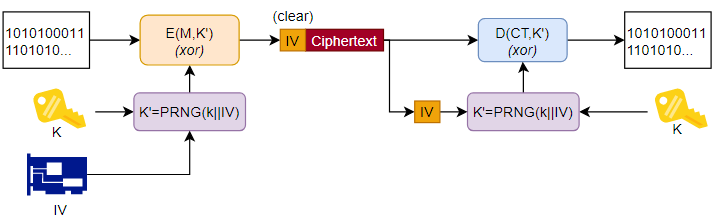
\includegraphics[width=\textwidth]{image/streamIV.png}
    \caption{Stream Ciphers with IV}
    \label{fig:streamiv}
\end{figure}\\
Abbiamo diversi modi per generare degli IV che siano sempre nuovi, al fine di applicare lo schema in \cref{fig:streamiv}:

\begin{itemize}
    \item \textbf{(Truly) Random:} ovvio. Di positivo ha che non può essere predibile, ma non realizzabile se non affidandosi ad effettive fluttuazioni naturali.
    \item \textbf{Sequence Number:} un numero di sequenza può essere sempre nuovo, ma può essere predetto, ad esempio identificando dopo quanti cicli la sequenza inizia a ripetersi; basta catturare un numero sufficiente di pacchetti o fare in modo di individuare i momenti in cui la rete si riavvia, per sincronizzarsi con la scheda in trasmissione.
\end{itemize}

\section{WEP: errori di design}
Il sistema WEP (Wired Equivalent Privacy) era il sistema di sicurezza adottato all'inizio dei sistemi WiFi, prima di WPA/WPA2; Consisteva in uno stream cipher basato su RC4 (State-of-Art per il tempo, oggi obsoleto) per generare il keystream. 
\begin{center}
    $ENC(K,MSG)=MSG\oplus{RC4(IV,K)}$
\end{center}
Tuttavia, in WiFi c'è un grosso problema legato alla perdita dei pacchetti durante una trasmissione, pertanto, suddividendo il messaggio in diversi pacchetti, per ognuno di questi pacchetti è necessario generare un nuovo keystream (ovvero un nuovo IV) e inoltre è necessario riconoscere il punto di perdita per ricominciare a trasmettere.\\
\begin{remark}
Tanti pacchetti significano tanti inizialization vector: anche usando numeri randomici, con pochi bit abbiamo tanta ripetizione. Usare numeri di sequenza non è praticabile in quanto sarebbe facilmente sincronizzabile.\\
Se collezionando i pacchetti un attaccante dovesse cominciare a fare uno $xor$ di due messaggi potrebbe risalire alla chiave, risultando sensibile ad attacchi di tipo CPA o KPA \textit{(known plaintext attack)}
\end{remark}\pagebreak
\subsection{Errori di Confidentiality}
Riguardo alla confidentiality, i problemi furono principalmente due:
\begin{enumerate}
\item \textit{Lunghezza IV troppo corta}: 24bit. La probabilità che l'IV si ripetesse in pochi frame era alta e, difatti:
$24\text{bit}\rightarrow{2^{24}=16.777.216} \text{frames}$.\\Assumendo di inviare $1500\text{byte/frame}\sim7\text{Mbps}$, in circa 8 ore si può trovare la chiave. Inoltre, è stato dimostrato che aumentare la dimensione della chiave non risolveva il problema, poiché l'attacco scala linearmente con la lunghezza dell'IV.
\item \textit{Generatore di IV lasciato all'implementazione:} Lo standard non definiva il modo con cui gli IV dovessero essere generati, esponendo il sistema ad un utilizzo inesperto o improprio. Ad esempio, mettere tutti 0 o tutti 1 come keystream annienta la sicurezza in quanto lo xor di quei due stream fa sì che non venga cifrato lo stream key+IV. Ciò non toglie il fatto poi che basta un semplice reboot del sistema a re-inizializzare a tutti 0 l’IV (ripetizione).
\end{enumerate}
Un attaccante, banalmente collezionando i pacchetti, poteva costruire un dizionario di coppie IV-keystream ed individuare lo schema di generazione, deducendo la chiave.
\subsection{Errori di Authentication}
Diamo prima una definizione di autenticazione:
\begin{definition}[Authentication]
L'autenticazione è un servizio essenziale nella sicurezza che consiste provare la propria identità digitale. Essa consiste nel provare che le credenziali di un individuo siano autentiche. Un'autenticazione andata a buon fine è tale se riesco ad essere sicuro che il soggetto che accede al servizio in un dato momento è lo stesso che ha acceduto in passato.
\end{definition}
\begin{proposition}[Mezzi di Autenticazione]
Alcuni mezzi di autenticazione sono:
\begin{itemize}
    \item \textbf{Conoscenza di un segreto:} Password, PIN, chiave; Dimostro di conoscere un segreto.
    \item \textbf{Possesso esclusivo di un requisito fisico:} Dimostro di avere qualcosa (smart card o dispositivi fisici), autenticazione basata su unicità di un hardware (Physically Unclonable Function).
    \item \textbf{Autenticazione biometrica:} Dimostrare di essere qualcuno sulla base del proprio DNA (impronta digitale e simili).
    \item \textbf{Biometrica dinamica:} Azioni di un soggetto, riconoscimento della voce, calligrafia o movenze.
\end{itemize}
\end{proposition}
L'idea di \textit{WEP} non era quella di autenticare realmente gli utenti, ma di costruire un database di chi poteva avere accesso alla rete. Tutti gli autorizzati nella rete avrebbero potuto comunicare senza ausilio crittografico, mentre chi si trovava fuori la rete avrebbe osservato invece tutto cifrato. Da qui la definizione di \textbf{“Wired equivalent privacy”}, ovvero la conoscenza di un segreto rende un utente fidato.\newpage
Il processo di autenticazione era di tipo \textit{challenge}, \textbf{con la stessa chiave pubblica}. Ovvero:
\begin{enumerate}
    \item L'access point invia un valore numerico in chiaro all'utente. Quel numero consiste nella \textbf{challenge} da soddisfare.
    \item L'utente che accede invia all'access point un pacchetto contenente l'IV (deciso dall'utente), in chiaro, e la challenge cifrata tramite \textit{xor} con $RC4(IV,K)$.
\end{enumerate}
\begin{figure}[h]
    \centering
    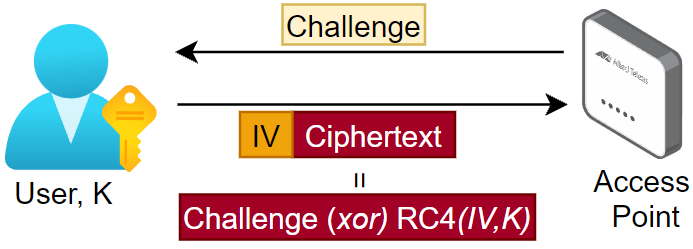
\includegraphics[width=0.8\textwidth]{image/wepchallenge.png}
    \caption{Authentication in WEP}
    \label{fig:wepchallenge}
\end{figure}
Dato che la chiave è pubblica, l'access point può verificare la conoscenza della chiave da parte dell'utente semplicemente eseguendo a sua volta lo \textit{xor}, applicando $RC4$ all'IV spedito in chiaro.\\
Le debolezze di questo sistema di auth sono le seguenti:
\begin{enumerate}
    \item Inviando la challenge in chiaro, se si dispone della relativa risposta, eseguendo \[Ciphertext\oplus{Challenge}=RC4(IV,K)\]
    si può derivare il keystream e da li è possibile produrre pacchetti firmati senza conoscere la chiave.
    \item Poiché l'initialization vector è deciso dall'implementatore, l'access point non ha modo di capire se la persona che invia la richiesta di auth è fidata. Difatti, eseguendo:
    \[
    Challenge\oplus{Challenge\oplus{RC4(IV,K)}}=RC4(IV,K)
    \]
    Esponiamo il keystream e permettendo diversi attacchi.
\end{enumerate}
Dal punto 1, capiamo che WEP finisce per implementare un KPA in quanto chiunque conosce la challenge può, costruendo un dizionario di coppie $(IV,RC4(IV,K))$, attendere che un IV si ripeta e violare il sistema.\\
Dal punto 2, si può vedere che un MITM in ascolto sul canale, può introdursi nella rete al primo IV che trova riscontro nel dizionario e da quel momento in poi restare autenticato per tutto il tempo che vuole, in quanto sarà sempre lui a decidere quale sarà l'IV da usare.\\
\begin{remark}
Una possibile soluzione, sarebbe potuta essere quella di \textbf{inviare l'IV insieme alla challenge}, in modo tale da non lasciare spazio agli utenti.
\end{remark}\pagebreak
\subsection{Errori di Integrity}
Esistono diversi algoritmi per garantire l'integrità di un pacchetto. WEP al tempo implementava $CRC-32$, un un algoritmo di error detection che può tener conto dei bit di partenza tramite bit di parità (posti alla fine del messaggio).
\begin{theorem}
$CRC-32$ è lineare nelle operazioni di $\oplus$. E' possibile modificare precisi bit del plaintext per produrre lo stesso checksum del messaggio non modificato.
\end{theorem}
\begin{proof}
La struttura del pacchetto WEP era costituita dal messaggio $M$ seguito dal codice di integrità $CRC32(M)$. Quando il messaggio viene inviato, tutti i bit vengono criptati nel seguente modo:
\[
C= M|CRC32(M)\oplus{RC4(IV, K)}
\]
Consideriamo un vettore $\delta$ di bit, lungo quanto M e contenente 1 nelle posizioni dei bit che si intende modificare nel messaggio originale.\\
Calcoliamo $CRC32(\delta)=c(\delta)$ e calcoliamo infine:
\begin{equation*}
    \begin{aligned}
    C'&=C\oplus\{\delta,c(\delta)\}\\
    &=[RC4(IV,K)\oplus{\{M,c(M)\}}]\oplus\{\delta,c(\delta)\}\\
    &=RC4(IV,K)\oplus\{M\oplus{\delta},c(M)\oplus{c(\delta)}\}\\
    &=RC4(IV,K)\oplus\{M',c(M\oplus{\delta})\}\\
    &=RC4(IV,K)\oplus\{M',c(M')\}
    \end{aligned}
\end{equation*}
Vediamo quindi che unendo al messaggio cifrato la concatenzazione $\{\delta,c(\delta)\}$ la parità misurata dall'algoritmo di controllo non risulta alterata grazie alla parità.
\end{proof}
\begin{remark}
In sintesi, il fatto che $CRC(32)$ sia lineare, risulta una debolezza per il sistema.
\end{remark}
\begin{proposition}
Un buon sistema di integrità dovrebbe garantire che:
\begin{enumerate}
    \item L'integrity checker deve essere non lineare.
    \item l'integrity checker deve esplicitamente includere una chiave, in quanto cifrature esterne non forniscono alcuna garanzia.
\end{enumerate}
\end{proposition}
\begin{remark}
Se si volesse tentare un attacco di tipo \textbf{\textit{Message Injection}} di un messaggio $M$ sarebbe ancora più facile. Una volta ottenuta una coppia valida di $(IV,RC4(IV,K))$ basta calcolare $c(M)$ e inviare $[M,c(M)]$ in xor con la la firma.
\end{remark}
\chapter{MSG Authentication come MSG Integrity}
Abbiamo visto che garantire la confidenzialità dell'informazione di un pacchetto non significa garantire anche la sua integrità. Questo significa che non abbiamo garanzie che un sistema che fornisce una corretta cifratura sia anche inattaccabile al suo interno tramite l'inserimento di un messaggio malevolo. In sintesi:
\begin{itemize}
    \item Confidenzialità significa nascondere il contenuto di un messaggio per un esterno, con la sicurezza che soltanto il destinatario può leggerlo.
    \item Integrità significa autenticità del messaggio, ovvero la sicurezza che nessuno possa modificare il messaggio. Né estendendolo, né disturbandolo (questo potrebbe anche essere a problemi di telecomunicazione, che tralasciamo)
\end{itemize}
Queste osservazioni sono vere sempre, a meno di parlare di AEAD (\ref{def:aead}). In generale, quello che vogliamo è la sola integrità. 
\begin{example}[ Il Curriculum] chiunque dovrebbe essere in grado di leggerlo, solo il proprietario dovrebbe essere in grado di modificarlo.
\end{example}
\begin{example}[ Integrità del One Time Pad]
Sappiamo che il One Time Pad (vernam cipher) è il miglior cifratore possibile, se le sue ipotesi sono rispettate. Eppure, se un'attaccante modificasse un cipher-text, l'uscita sarebbe diversa. Infatti:
\begin{figure}[hb]
    \centering
    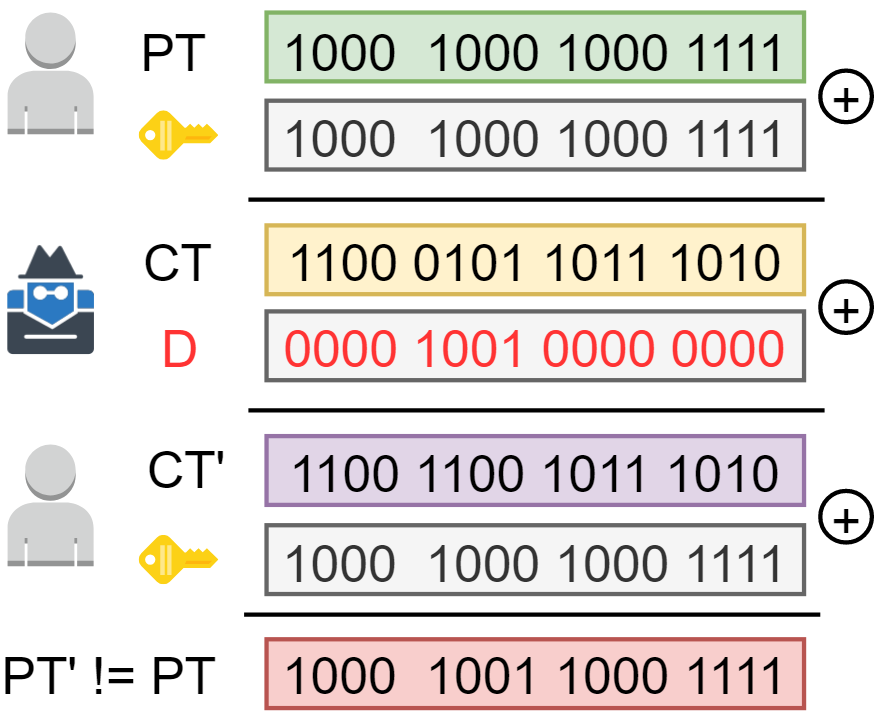
\includegraphics[width=0.5\textwidth]{image/vernaminteg.png}
    \caption{Fallimento del Vernam Cipher}
    \label{fig:vernamfail}
\end{figure}
\end{example}\pagebreak
\section{Message Authentication con Chiave Simmetrica}
Supponiamo che Sender e Receiver conoscano una chiave $K$ usata \textbf{\textit{esclusivamente}} per il servizio di integrità. Vogliamo aggiungere al messaggio un pacchetto che serva da \textbf{integrity check}. Chiamiamo \textbf{\textit{TAG}} questa aggiunta.\\
Un modo per generare questo TAG è quello di usare una funzione hash che leghi il messaggio da inviare con la chiave, producendo un \textbf{\textit{digest}} che farà appunto da TAG. Poiché la chiave è simmetrica, il ricevitore sarà in grado di generare un suo tag che potrà confrontare con quello inviato dal Sender. Se c'è un matching tra i due tag, allora il messaggio è necessariamente autentico. 
\begin{figure}[h]
    \centering
    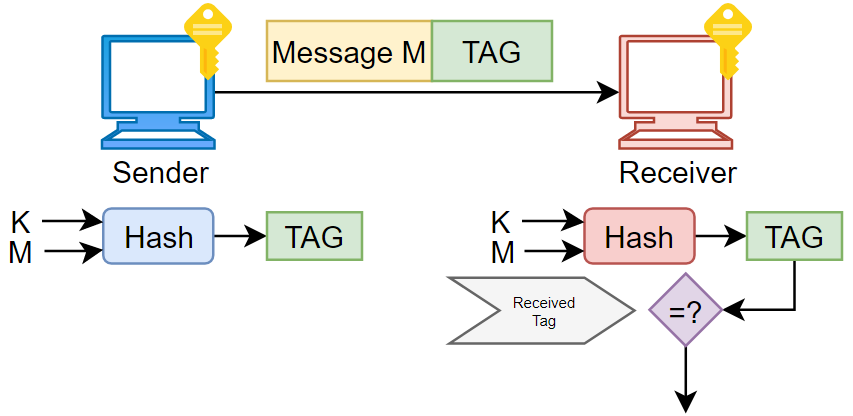
\includegraphics[width=0.8\textwidth]{image/integrityscheme.png}
    \caption{Integrity Check Scheme}
    \label{fig:intcheck}
\end{figure}
\subsection{Message Authentication Code}
I message authentication code sono una forma più debole di firma digitale \textit{(Digital Signature)}. Nella DS nessuno può modificare un messaggio a parte chi l'ha firmato. Con il MAC solo il sender ed il receiver possono farlo; Questo perché entrambi conoscono la chiave.\\
Una definizione possibile di sicurezza per un sistema di autenticazione è:
\begin{definition}[Unforgeability]\label{def:unforge}
Un messaggio sicuro ed autenticato è inforgiabile, nel senso che un attaccante non deve essere né capace di creare né di modificare un messaggio.\\
Quindi, dati all'attaccante un numero di messaggi passati, non può generare un tag valido o almeno la probabilità di riuscire a forgiare una coppia messaggio/tag autonomamente deve essere praticamente nulla (negligible). 
\end{definition}
\begin{remark}
Data la definizione \ref{def:unforge}, escludiamo l'idea di utilizzare un tag corto, in quanto l'unica possibilità dell'attaccante è provare ad indovinare la coppia. Avere un tag lungo implica più meno probabilità di indovinare un numero casuale.\\
Tipicamente, la lunghezza considerata minima per avere un tag sicuro è di 96bit.
\end{remark}
\subsection{Vulnerabilità ai Man In The Middle Attacks}
Supponiamo che un attaccante possa intercettare la coppia $(MSG,TAG)$ di un Sender e volesse modificare il messaggio $M$ in $M'$. Se la funzione hash è considerata \textbf{crittograficamente forte}, allora:
\begin{itemize}
    \item L'attaccante non è capace di calcolare la chiave in quanto $H(\cdot)$ non è invertibile.
    \item l'attaccate non deve essere in grado di alterare il tag, in modo tale che $tag'=H(K,M')$ senza conoscere $K$
    \item L'attaccante non deve essere capace di cambiare $M$ in $M'$ in modo tale che \[H(K,M)==H(K,M')\]
\end{itemize}
Poiché non è possibile prevenire un MITM, il tag fornisce un valido aiuto nell'intercettare un attacco in corso o avvenuto, in quanto il tag risultarà alterato.
\subsection{Vulnerabilità ai Reply Attacks}
I reply attacks consistono nel seguente schema: se vengono mandati due messaggi identici, i tag risultanti saranno identici.
\begin{proposition}\label{prop:macreplay}
I MAC non proteggono dai reply attack, \textbf{a meno che i messaggi non si ripetano mai.}
\end{proposition}
Un esempio tipico di reply attack sono i message spoofing:
\begin{definition}[Message Spoofing]
Attacco nel quale il messaggio viene mandato dall'attaccante, ma spacciato per un altro mittente, senza che il destinatario se ne accorga.
\end{definition}
Consideriamo i due piani su cui si svolge la comunicazione tra due utenti, l'applicativo e quello protocollare (il vero responsabile della comunicazione). Supponendo che lo strato applicativo sia ben implementato (i messaggi non si ripetono), è il protocollo che deve garantire la sicurezza.\\
Il modo con cui possiamo garantire la non ripetibilità a livello protocollare è specificare il modo con cui generiamo il numero randomico che, unito alla chiave, genera il tag. Diamo una rapida revisione:
\begin{table}[ht]
    \centering
    \begin{tabular}{ |p{0.2\textwidth}|p{0.7\textwidth}|  }
    \hline
    \textbf{Tipo}&\textbf{Conseguenza}\\
    \hline
    Sequence Number & Riavviando il sistema si azzera il contatore e potrebbe ripetersi.\\
    \hline
    Random Number & Ottimo, specialmente se sono true random. Potrebbe esserci un problema di collisione a seconda del numero di bit usati. Inoltre, se c'è collisione, non possiamo capire se un pacchetto si è ripetuto senza memorizzarli pertanto non è una soluzione scalabile.\\
    \hline
    Time stamp & Il problema di questo è che il tempo deve essere garantito come dato certo. Il NTP (network time protocol) non garantisce integrità. Il riferimento usato dall'operatore telefonico potrebbe essere disturbato con un segnale radio e cambiato.\\
    \hline
    \end{tabular}
\end{table}
\section{Funzioni Hash Crittografiche}
Per costruire un MAC abbiamo bisogno di 2 ingredienti:
\begin{enumerate}
    \item Una buona funzione hash (es: SHA256)
    \item Includere il segreto nella funzione hash
\end{enumerate}
\subsection{Caratteristiche di una Cryptografic Hash Function}
A meno di non possedere una funzione hash perfetta, ovvero un random oracle, è importante dove posizionare il segreto rispetto al messaggio all'interno della funzione. Tipicamente, lo schema di una funzione hash è questa:
\begin{figure}[h]
    \centering
    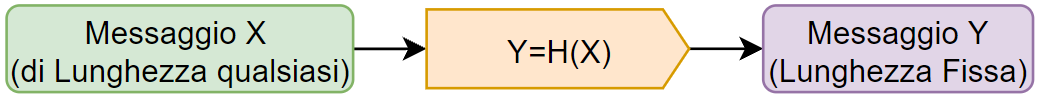
\includegraphics[width=\textwidth]{image/hashscheme.png}
    \caption{Schema di una Funzione Hash}
    \label{fig:hashscheme}
\end{figure}\\
Una funziona hash è crittografica se soddisfa tre diverse proprietà, che rendono impossibile per un attaccante creare o modificare/estendere/rimpiazzare il messaggio di partenza per ottenere un digest valido. 
\begin{theorem}[Preimage Resistance]\label{thm:preimageres}
Dato il risultato di un hash $Y=H(X)$ è difficile trovare un valore qualsiasi di $X\,:\,H(X)=Y$
\end{theorem}
Questo significa che una funzione hash crittografica deve essere resistente ad attacchi brute-force, pertanto, \textbf{la dimensione del digest è importante}. 
\begin{example}
Supponendo di avere un digest di 16bit, abbiamo $2^{16}$ possibili combinazioni di $0$ ed $1$, ovvero la probabilità di indovinare è $\frac{1}{2^{16}}$. Supponendo di disporre di una macchina in grado di elaborare $66$ Mhash/sec in meno di un millisecondo avremo trovato una soluzione.
\end{example}
\begin{remark}
Se dovessero esserci dei bit correlati nella sequenza di bit del digest, per ogni relazione ridurremmo la complessità del calcolo di un fattore 2, ovvero la complessità ha una decrescita esponenziale. Ad esempio, una chiave di $2^{10}$bit ha $1024$bit di complessità computazionale. Quindi, per ogni 10bit, aggiungiamo un fattore $1000$ di complessità.
\end{remark}
\begin{theorem}[Second Preimage Resistence\footnotemark]\label{thm:weakcollres}
Dato un numero $X$, è difficile trovare un numero $X'\,:\,H(X)=H(X')$
\footnotetext{\textsuperscript{\thefootnote}Detta anche Weak Collision Resistence}
\end{theorem}
\begin{example}
Un esempio di funzione che soddisfa la proprietà 1 ma non la 2 è $y(x)=g^x\bmod{p}$, dove $g$ è un numero noto, non necessariamente grande, e $p$ è un numero primo grande. Per trovare $x$ esistono algoritmi che in tempo esponenziale risolvono il problema\footnotemark.\\
Si può dimostrare che \[g^x+(p-1)k\bmod{p}=g^x\bmod{p}\,\forall{k}\] e la proprietà 2 è violata.
\footnotetext{Discrete Logarithm Problem} 
\end{example}
\begin{theorem}[Collision Resistence\footnotemark]\label{thm:strongcollres}
E' difficile trovare due numeri generici $X_1,X_2$ tale che $H(X_1)=H(X_2)$
\footnotetext{\textsuperscript{\thefootnote}Detta anche Strong Collision Resistence}
\end{theorem}
Vediamo un esempio importante per comprendere la terza proprietà:
\begin{example}[ Il Paradosso del Compleanno]
Dato un numero $N$ di persone, e presa una data di nascita, la probabilità che qualcuno \textbf{NON }sia nato nello stesso giorno è
\begin{equation*}
    \bigg(1-\frac{1}{365}\bigg)^K=\bigg(\frac{364}{365}\bigg)^K;\,\,\,K=N-1
\end{equation*}
In una classe di $N=23$ persone, selezionata una data, restano 22 possibili date, quindi $K=22$ e abbiamo il $\left(\frac{364}{365}\right)^{22}=94.1\%$. Ovvero, abbiamo il $6\%$ di possibilità che ci siano due persone nate lo stesso giorno.\\
Mantenendo lo stesso numero $N$, consideriamo ora la probabilità che \textbf{due persone} siano nate nello stesso giorno.
\begin{equation*}
    {1}\cdot\left({1}-\frac{{1}}{{365}}\right)\cdot\left({1}-\frac{{2}}{{365}}\right)\cdot\cdot\cdot\left({1}-\frac{{22}}{{365}}\right)={49.3}\%
\end{equation*}
\textbf{Abbiamo circa il $50\%$ di possibilità che ci siano due persone nate lo stesso giorno}.
\end{example}
In un contesto di crittografia, possiamo sostituire lo stesso giorno di nascita con una collisione di una funzione hash, che può dare lo stesso output per due input diversi. 
\begin{theorem}[Matematica del Paradosso del Compleanno]
Consideriamo un digest di $n$bit. Il numero di messaggi che possiamo produrre è $N=2^n$. Supponendo di avere a disposizione $K$ messaggi e che $p$ sia la probabilità che ci sia una collisione, la probabilità che \textbf{non ci siano collisioni} è:
\begin{equation}\label{eq:birthdayparadox}
    P(no\,coll.)=1-p=\frac{N!}{N^K(N-K)!}
\end{equation}
\end{theorem}
\begin{proof}Espandendo la formula \cref{eq:birthdayparadox}, risulta:
\begin{equation*}\begin{aligned}
    P&=
    \frac{N}{N}\cdot\frac{N-1}{N}\cdot\frac{N-2}{N}\cdot\dots\cdot\frac{N-(K-1)}{N}\\
    &=1\cdot\left(1-\frac{1}{N}\right)\cdot\dots\cdot\left(1-\frac{K-1}{N}\right)\\
    &=\prod_{i=1}^{K-1}\left(1-\frac{i}{N}\right)\approx
    \prod_{i=1}^{K-1}e^{\frac{-i}{N}}=e^{-\frac{\prod_{i=1}^{K-1}i}{N}}\\
    1-p&=e^{-\frac{K(K-1)/2}{N}}\approx{e^{-\frac{K^2}{2N}}}
\end{aligned}
\end{equation*}
Risolvendo in $K$ per calcolare il numero di messaggi affinché la probabilità di collisione sia del $50\%$, ovvero $p=\frac{1}{2}$, e ricordando che $N=2^n$ :
\begin{equation*}
    \log(1-p)\approx{-\frac{K^2}{2N}}\Longrightarrow{K=\sqrt{2N}\cdot{\sqrt{\log\left(\frac{1}{1-p}\right)}}}
\end{equation*}
\[K\approx{\sqrt{2}\cdot\sqrt{2}\sqrt{N}}\approx{1.177\sqrt{N}}\approx{1.777\sqrt{2^N}}\approx2^{\frac{n}{2}}\]
\end{proof}
\begin{proposition}[Collision Resistence Level]
Dato un digest di $n$ bit, la probabilità di avere una collisione del $50\%$ avviene dopo $2^{\frac{n}{2}}$ messaggi..
\end{proposition}
Dalla proposizione $3.2$ capiamo che la dimensione del digest deve essere impostata per ovviare al \textit{birthday paradox}. Alcuni esempi di quanto incide la dimensione su un attacco brute-force sono i seguenti:
\begin{itemize}
    \item Random 32 bits: 4.3 miliardi di output. \textbf{$50\%$ di collisione dopo $2^{16}\approx60.000$ messaggi}.
    \item MD5, 128 bits: \textbf{$50\%$ di collisione dopo $2^{64}=1.8\times10^{19}$} (debole oggi). Inoltre, l'algoritmo è stato rotto nel 2005.
    \item SHA256, 256 bits: \textbf{$50\%$ di collisione dopo $2^{128}=3.4\times10^{38}$}. Ok al giorno d'oggi, richiederebbe almeno un miliardo di secoli per l'intera rete di bitcoin mondiale.
\end{itemize}
\subsection{Inserire un Segreto in un Hash}\label{sub:secretpos}
Poiché il segreto è solitamente la stessa chiave di autenticazione, è computazionalmente difficile per un attaccante costruire un MAC valido. Per come abbiamo definito le funzioni hash crittografiche, un cambiamento nel messaggio in ingresso equivale ad un cambiamento del messaggio in uscita.
\begin{remark}
Il punto di inserimento del segreto è fondamentale, in quanto cambia il risultato del digest. Inoltre, la sua posizione rende più o meno sensibili a diversi tipi di attacchi.
\end{remark}
Supponiamo di usare una buona funzione hash, come SHA256.
\begin{definition}[SHA256]
L'algoritmo SHA256 si basa sull'\textit{Iterative Merkle-Damgard Construction}, un teorema che garantisce che se la funzione di compressione è sicura, tutta la costruzione è sicura.\\
Prende in input $K$ bit arbitrari, aggiungendo un padding formato da $1$ seguito da tanti $0$ per formare un messaggio di $N\times512$bits. Tra gli ultimi 64 bit, viene inserito un numero corrispondente alla lunghezza del messaggio. Vedi \cref{fig:sha256}\\
Il digest viene prodotto con un rapporto di compressione di 3:1, fornendo un IV da 256bits in ingresso, che viene elaborato con uno dei blocchi da 512bits. Il risultato della funzione è un blocco di 256bits che viene fornito come IV al prossimo anello della catena.
\end{definition}
\begin{note}Gli IV disponibili per SHA256 sono delle costanti ben definite da standard.\end{note}
Vediamo come cambia il livello di sicurezza in funzione della posizione del segreto:
\begin{itemize}
    \item \textbf{Segreto alla FINE del messaggio:} l'attaccante potrebbe calcolare una sola volta la prima parte del messaggio e provare tutte le combinazioni possibili per la compressione dell'ultimo blocco. Questo riduce la complessità del brute-force attack e, quindi, della sicurezza. Vedi \cref{fig:secretprecomp}
    \item \textbf{Segreto all'INIZIO del messaggio:} inserire il segreto all'inizio permette di eseguire un message-extension attack. All'attaccante è sufficiente calcolare il padding e la lunghezza (ultime parti del messaggio) ed inserire alla fine un plaintext arbitrario, creando un nuovo chunk tale che riapplicando la funzione di compressione si ottiene un messaggio valido \textbf{non scritto dall'utente}. Vedi \cref{fig:macmsgext}
\end{itemize}
\begin{note}
    In questo caso l'attaccante non serve che conosca il segreto per sfruttare la vulnerabilità.
\end{note}
\begin{figure}[h]
    \centering
    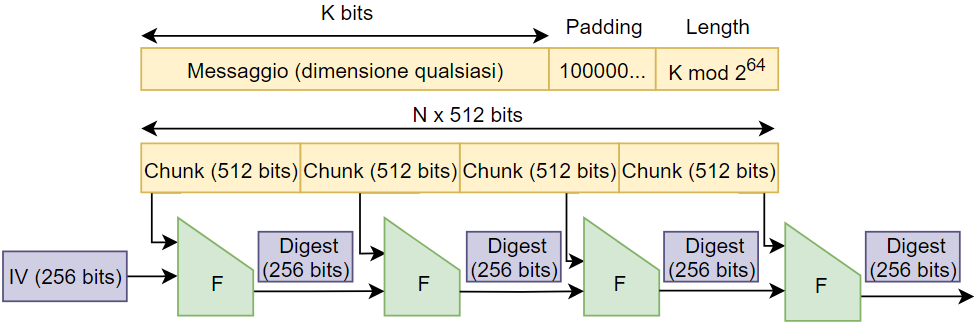
\includegraphics[width=0.9\textwidth]{image/sha256.png}
    \caption{SHA256 hash scheme}
    \label{fig:sha256}
\end{figure}
\begin{figure}[h]
    \centering
    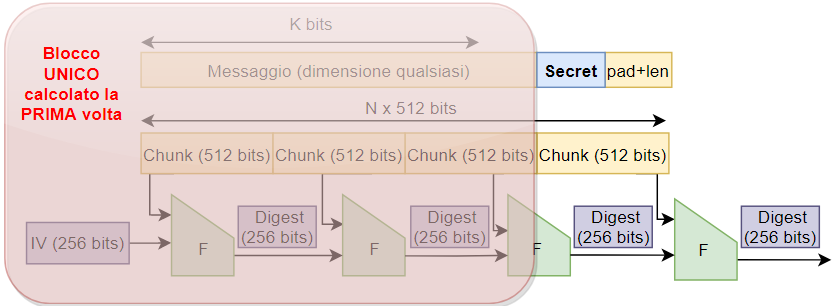
\includegraphics[width=0.9\textwidth]{image/stateprecomp.png}
    \caption{Precomputation con Segreto alla fine}
    \label{fig:secretprecomp}
\end{figure}
\begin{figure}[h]
    \centering
    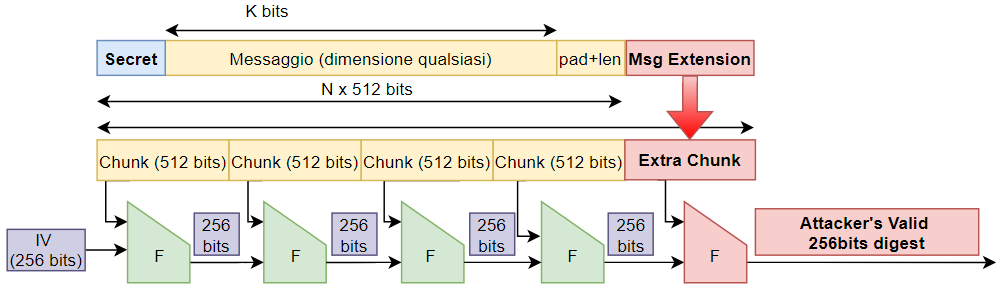
\includegraphics[width=0.9\textwidth]{image/macmsgext.png}
    \caption{Message Extension Attack example}
    \label{fig:macmsgext}
\end{figure}
\section{Hash Based Message Authentication Code}
Abbiamo visto che una funzione hash che risulta sicura dal punto di vista crittografico (cioè valgono: \cref{thm:preimageres,thm:weakcollres,thm:strongcollres}) non è sufficiente a garantire l'integrità di un messaggio. Esiste però una costruzione che può rendere il tag perfettamente sicuro. 
\begin{definition}[HMAC Construction]\label{def:hmac}
Dato un segreto $K$ pre-condiviso, e scelta una funzione hash $H$ che rispetta le ipotesi descritte da \cref{thm:preimageres,thm:weakcollres,thm:strongcollres}, si crea un codice di autenticazione per un messaggio $M$ con la seguente costruzione:
\begin{equation}\label{eq:hmac}
HMAC_K(M)=H[K^+\oplus{\text{opad}}||H(K^+\oplus{\text{ipad}}||M)]
\end{equation}
Dove con $K^+$ indichiamo l'estensione della chiave $K$ alla dimensione di block-size necessaria alla funzione hash $H$ aggiungendo un padding di zeri. I numeri $opad$ e $ipad$ sono due costanti, ripetute quanto serve, definite da standard rispettivamente come:
\begin{itemize}
    \item $\textbf{opad}=0\times36=00110110$
    \item $\textbf{ipad}=0\times5C=01011100$
\end{itemize}
\end{definition}
\begin{figure}[h]
    \centering
    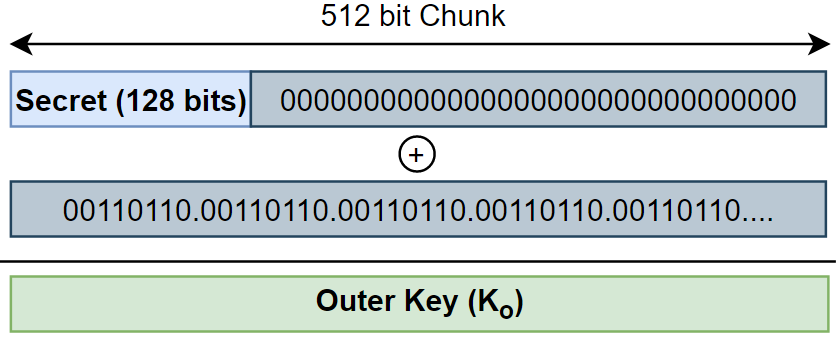
\includegraphics[width=0.6\textwidth]{image/hmackplus.png}
    \caption{SHA256 Key Extension with Outer Pad}
    \label{fig:hmackplus}
\end{figure}
\begin{figure}[h]
    \centering
    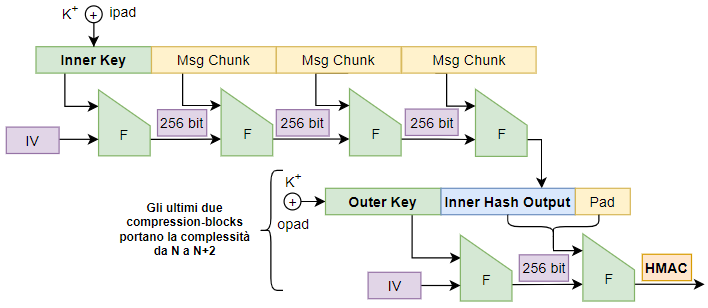
\includegraphics{image/hmac.png}
    \caption{HMAC-SHA265 construction}
    \label{fig:hmacsha256}
\end{figure}
La costruzione di HMAC si basa quindi sul possesso di un singolo segreto che viene messo in xor in due modi diversi, per garantire che le due chiavi usate nell'hashing siano diverse. Sebbene l'inner hash prodotto da $H(K^+\oplus{\text{ipad}}||M)$ sia vulnerabile ad extension attack (\cref{fig:macmsgext}, la costruzione rende impossibile produrre un tag valido perché il digest finale prodotto dai 2 blocchi aggiuntivi non può essere esteso. Inoltre, la complessità per individuare la chiave tramite brute-force è pari a N blocchi più i due aggiuntivi dall'hash esterno. 
\begin{note}
    HMAC è più sicuro di una generica hash function. Inoltre, anche se la funzione hash presenta dei problemi di collisione, la costruzione risulta ancora sicura, anche se la collisione è calcolabile.
\end{note}

\chapter{User Authentication}
Consideriamo uno scenario in cui è necessario autenticare un utente all'interno del sistema. Al giorno d'oggi confondiamo il concetto di password con quello di segreto, in quanto una password rappresenta la base usata dalla maggior parte dei sistemi di autenticazione moderni. In un contesto di sicurezza, tuttavia, è bene separarli:
\begin{itemize}
    \item \textbf{Segreto:} Sequenza di bit costituita da un numero qualsiasi di caratteri. Tipicamente ad \textit{\textbf{alta entropia}}.
    \item \textbf{Password:} Stringa di caratteri, solitamente alfanumerici, caratterizzata da una \textbf{\textit{bassa entropia}}.
\end{itemize}
Un modo possibile di vedere l'entropia di un oggetto è come una quantità che rappresenta una stima di quanta casualità esso contiene. Per il nostro contesto, ci viene in aiuto il seguente teorema:
\begin{theorem}[Shannon Entropy]\label{thm:shannonentropy}
Sia $X$ una variabile aleatoria discreta, costituita da un numero $n$ di caratteri ognuno dotato di probabilità di apparire pari a $p_i,\,i=1,\dots,n$. Definiamo il valore, \textbf{in bit}, dell'entropia di $X$ come:
\begin{equation}\label{eq:entropy}
H(X)=-\sum_{i=1}^{n}p_i\log_{2}\left(p_i\right)
\end{equation}
\end{theorem}
\begin{proposition}[Information Content]
Il valore informativo dell'evento $x_i$ dipende da quanto lo stesso $x_i$ è inatteso, ovvero, il contenuto informativo è funzione di $\frac{1}{p_i}$.\\
Considerando gli eventi come possibili valori di un bit, se un evento ha probabilità di apparire con $p=\frac{1}{2^b}$ l'information content vale: 
\begin{equation}
    IC_i=-\log_{2}\left(\frac{1}{2^b}\right)=b \,\text{bits}
\end{equation}
\end{proposition}
\begin{corollary}
Possiamo vedere l'entropia come il valor medio dell'information content di una variabile aleatoria: 
\begin{equation}
    H(X)=E[IC(X)]=\sum_{i}^{n}p_i IC_i=-\sum_{i=1}^{n}p_i\log_{2}\left(p_i\right)
\end{equation}
\end{corollary}
\begin{note}
Per un insieme di $N$ eventi, l'entropia può andare da 0 ad $N$, a seconda della probabilità degli eventi stessi. 
\begin{itemize}
    \item Se l'entropia è nulla abbiamo un caso di \textbf{"Minima Entropia"}, ovvero l'evento è deterministico.
    \item Se l'entropia è $N$ allora si ha \textbf{"Massima Entropia"} e ogni evento è equiprobabile.
    \item In tutti i casi intermedi, vuol dire che ogni evento non ha la stessa probabilità di accadere.
\end{itemize} 
\end{note}\pagebreak
\section{Password vs Segreto}
Tipicamente le password presentano 4 tipi di problemi diversi, difficilmente risolvibili.
\begin{definition}[Overload]
Riuso della stessa password per diversi siti.
\end{definition}
Infatti, da una statistica americana si evince che:
\begin{itemize}
    \item [\textcolor{blue}{$\Rightarrow$}]il 38\% degli utenti globali riusano stessa password su diversi siti, il che mette in pericolo la sicurezza.
    \item [\textcolor{blue}{$\Rightarrow$}]Risulta anche che il 21\% degli utenti che volendosi sentire più sicuri modificano la propria password, lo fanno in modo prevedibile.
\end{itemize}
\begin{definition}[Restricted Charset]
Le password sono tipicamente generate da tastiera e non tutti i caratteri sono usati:  sui 256 caratteri totali vengono usati solo i 102 fisicamente presenti.
\end{definition}
\begin{itemize}
    \item [\textcolor{blue}{$\Rightarrow$}]I caratteri ASCII sono codificati con 1 byte, ovvero una stringa di 8bit corrispondenti a $2^8=256$ possibilità. La probabilità di indovinare 1 bit è quindi di $\frac{1}{256}$. 
    \item [\textcolor{blue}{$\Rightarrow$}]Supponendo di avere un segreto di 8 byte, la probabilità è $\frac{1}{256^8}$.
    \item [\textcolor{blue}{$\Rightarrow$}]Usando solo caratteri alfanumerici \textit{lower-case}, con 1 byte copriamo al massimo 36 possibili valori. Pertanto la probabilità di indovinare 8 caratteri diventa $\frac{1}{36^8}$, che è \textbf{decisamente} inferiore.
\end{itemize}
\begin{definition}[Low Entropy]
Poiché tipicamente create con l'intento di essere ricordate, le password sono sequenze specifiche non propriamente random nella stragrande maggioranza dei casi.
\end{definition}
\begin{example}[ Bit Flip:]Consideriamo $X_k=\{0,1\}$ con probabilità $p_k=1/2$. L'entropia vale:\[H(X)=-\frac{1}{2}\log_{2}\left(\frac{1}{2}\right)-\frac{1}{2}\log_{2}\left(\frac{1}{2}\right)=\log_{2}(2)=1\,\text{bit}\]
\end{example}
\begin{example}[ Sequenza Indipendente di 3 bit:] Consideriamo $X_1,X_2,X_3$ con probabilità $p_k=1/2$. Abbiamo quindi in totale 8 sequenze diverse equiprobabili.
L'entropia vale: 
\[H(X)=-\sum_{i=1}^{8}\frac{1}{2^3}\log_{2}\left(\frac{1}{2^3}\right)=8\cdot\frac{1}{8}\cdot3=3\,\text{bit}\]
\end{example}
\begin{example} [ Coppia di bit Biased:] Consideriamo un bit $X_k=\{0,1\}$ i cui valori non sono a frequenza equa, ovvero capitano rispettivamente con probabilità $p_1=\frac{1}{4}$ e $p_2=\frac{3}{4}$
\[H(X)=-\frac{1}{4}\log_{2}\left(\frac{1}{4}\right)-\frac{3}{4}\log_{2}\left(\frac{3}{4}\right)=0.81\,\text{bit}\]
Questo significa che ogni bit trasmesso trasporta $0.81$bit di informazione e un'ipotetica sorgente di questo flusso di bit non potrebbe comprimere il suo messaggio più del $19\%$
\end{example}\pagebreak
\begin{example}[ Sequenza di 3 bit Dipendenti:] Consideriamo $X_1,X_2,X_3$ con probabilità $p_k=1/2$ e supponiamo che $X_2,X_3$ assumano lo stesso valore di $X_1$. Questo significa che abbiamo solo due casi possibili e l'entropia sarà:
\[H(X)=-\frac{1}{2}\log_{2}\left(\frac{1}{2}\right)-\frac{1}{2}\log_{2}\left(\frac{1}{2}\right)=\log_{2}(2)=1\,\text{bit}\]
Pertanto, solo 1/3 del messaggio trasmesso sarebbe il reale portatore di informazioni.
\end{example}
\begin{definition}[Predictability]
Solitamente una password viene scelta sulla base delle proprie esperienze o sulla base delle parole utilizzate da un individuo. Per attacchi mirati (\textit{\textbf{social engineering)}} o tramite collezione di password trovate per il web si possono indovinare facilmente.
\end{definition}
\begin{itemize}
    \item [\textcolor{blue}{$\Rightarrow$}]Le password sono soggette ai \textbf{Dictionary Attack}: L'idea è molto semplice, si prende un dizionario di parole comuni, sulla base di quelle che si dicono di solito o sui gusti comuni. Ci sono dei database di pubblico dominio di password ottenute da brecce eseguite in sistemi informatici, dove sono riportate anche le password più usate. 
    \item [\textcolor{blue}{$\Rightarrow$}]La tecnica di \textbf{Password spraying attack} è proprio l’azione di provare tutte le differenti password più utilizzate.
\end{itemize}
\begin{remark}
Abbiamo quindi capito che se i bit di una sequenza sono indipendenti, l'entropia aumenta, e viceversa. Poiché le password sono strutturalmente dotate di minore entropia rispetto ad un segreto, sono necessariamente meno sicure.
\end{remark}
\section{Authentication Protocols}
Un processo di autenticazione non è altro che una prova di conoscenza, nella quale si vuole dimostrare di conoscere una password o un segreto. 
\begin{note}
\textbf{Provare la propria conoscenza NON implica, necessariamente, rivelarne il soggetto.}
\end{note}
\subsection{Password Authentication Protocol (PAP)}
È l'approccio di autenticazione più semplice possibile e consiste nella trasmissione della password in chiaro sul mezzo di trasmissione, \textbf{all'inizio della sessione} (non viene mai ripetuta finché viene chiusa).
\begin{proposition}[PAP - Password Authentication Protocol]\label{prop:pap}
\begin{enumerate}
    \item L'utente in autenticazione invia un messaggio con \textit{(ID, PASSWORD)} all'authenticator, dotato di un database con scritte tutte le associazioni utente/password.
    \item L'authenticator controlla che i valori inviati di id e password corrispondano; In caso affermativo garantirà l’accesso.
\end{enumerate}
\end{proposition}
\begin{figure}[ht]
    \centering
    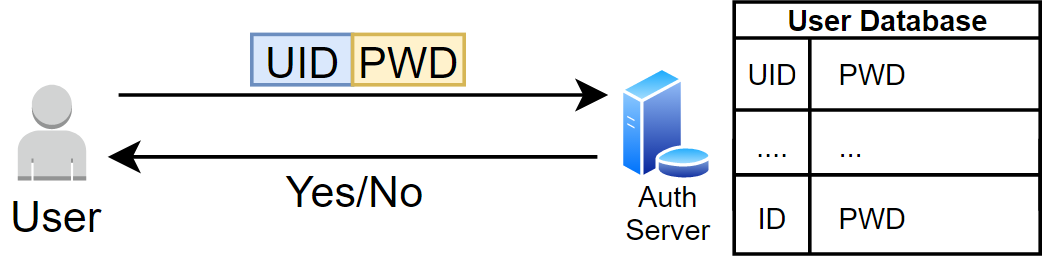
\includegraphics{image/pap.png}
    \caption{PAP scheme}
    \label{fig:pap}
\end{figure}
\begin{note}
\textbf{In PAP le password sono pre-condivise e trasmesse in chiaro ad ogni nuovo tentativo di autenticazione.}
\end{note}\pagebreak
E' facile notare che PAP ha delle limitazioni. In particolare:
\begin{itemize}
    \item  E' soggetto a \textbf{eaves-dropping:}la password e l'ID sono trasmessi in clear, se qualcuno ascolta mette a repentaglio la sicurezza. 
    \item Non c'è protezione da Replay Attack (ad un eventuale attacker basta ascoltare il messaggio che viene inviato all'authenticator per acquisire credenziali valide per entrare). 
    \item Il protocollo non specifica nulla sul numero dei tentativi per entrare (più tentativi a disposizione di un attacker gli garantiscono più possibilità di indovinare).
\end{itemize}
\subsection{Challenge Handshake Authentication Protocol (CHAP)}
Consiste in un approccio più conservativo dal punto di vista della sicurezza, in quanto la password non viene condivisa in chiaro come in PAP (\cref{prop:pap}) ma nascosta tramite una funzione hash.
\begin{remark}
E' necessario porre delle premesse sulla funzione hash usata da CHAP:
\end{remark}
\begin{itemize}
    \item Deve soddisfare le proprietà dei \cref{thm:preimageres,thm:weakcollres,thm:strongcollres}, in particolare la non invertibilità, altrimenti intercettando un messaggio basterebbe applicare la funzione inversa e decifrare la password.
    \item Seguendo le regole degli stream-ciphers, $H(\cdot)$ \textbf{NON} deve essere funzione della sola password $P$. Deve \textbf{SEMPRE} includere qualcosa di \textit{"fresco"}\footnotemark
\end{itemize}
\footnotetext{In genere una \textit{nonce}, ovvero qualcosa di unico, che può essere usato solo una volta.}
\begin{proposition}[CHAP - Challenge Handshake Authentication Protocol]\label{prop:chap}
\begin{enumerate}
    \item L'authenticator invia una \textbf{Challenge} (una \textbf{\textcolor{green}{nonce}}) all'utente, con il compito di \textbf{NON RIPETERE MAI} la challenge inviata.
    \item L'utente risponde con un messaggio contenente lo User ID e una \textbf{Response}:
    \[[UID,H(Challenge, Password, \text{altri oggetti utili}\footnotemark)]\]
    \item L'authenticator cerca nel database l'entry relativa all'UID. Poiché conosce la challenge, è in grado di calcolare l'hash della password e può controllare il valore della response rispetto a quello da lui calcolato. In caso affermativo garantirà l’accesso.
    \footnotetext{\textsuperscript{\thefootnote}Spesso vengono aggiunti altri oggetti utili all'autenticazione, poiché non danneggiano la robustezza della funzione Hash.}
\end{enumerate}
\end{proposition}
\begin{figure}[ht]
    \centering
    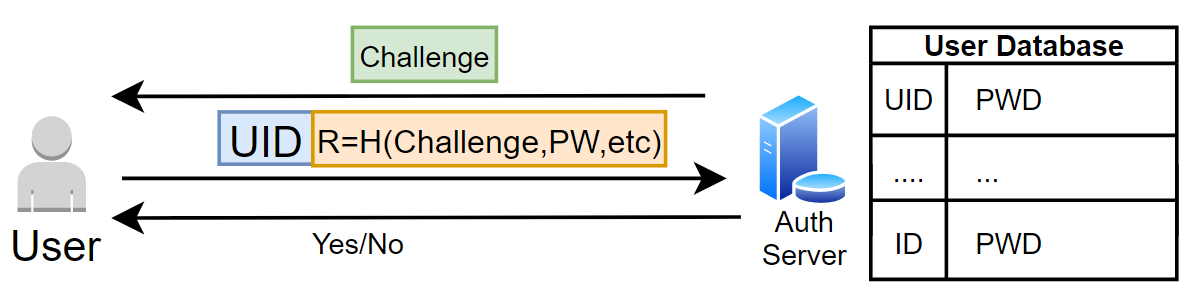
\includegraphics{image/chap.png}
    \caption{CHAP Scheme}
    \label{fig:chap}
\end{figure}
\begin{note}
Poiché abbiamo richiesto che $H(\cdot)$ non sia invertibile, CHAP sfrutta la conoscenza della challenge per consentire l'accesso. Se nella specifica applicazione vengono inviati ulteriori oggetti, l'authenticator dovrà usare anche quelli per calcolare l'hash.
\end{note}
Questo protocollo presenta diversi pro, ma anche un'importante controindicazione:
\begin{itemize}
    \item [\textcolor{green}{\checkmark}]CHAP protegge dai \textbf{replay attacks}, a patto che la challenge non si ripeta mai.
    \item [\textcolor{green}{\checkmark}]Poiché la challenge è decisa dall'ente preposto alla verifica, questo può:
    \begin{itemize}
        \item Controllare la frequenza e la tempistica con cui avvengono le richieste di autenticazione (utile per servizi di banca, ad esempio).
        \item Limitare il tempo di esposizione del sistema ad ogni singolo attacco, ad esempio imponendo un timer tra una richiesta di autenticazione e l'altra.
    \end{itemize}
    \item [\textcolor{red}{\ding{55}}]Il segreto deve essere disponibile nel database in formato plaintext, rendendo \textbf{impossibile} per un sistema che implementa CHAP salvare in DB delle password crittografate in quanto l'hash deve essere irreversibile e soprattutto la nonce deve essere sempre diversa.
\end{itemize}
\subsection{PAP vs CHAP - chi scegliere?}
Nonostante le applicazioni moderne usino PAP, per rispondere correttamente alla domanda su quale sia il miglior protocollo di autenticazione è importante considerare bene i modelli di attacco a cui possono essere sottoposti. 
\begin{theorem}[PAP vs CHAP]
Non esiste un'unica soluzione, \textbf{dipende da quale attacco ci si vuole difendere}.
\end{theorem}
Gli scenari principali sono due:
\begin{enumerate}
    \item \textbf{Attacco al Canale di Comunicazione} (eaves-dropping): Con PAP, è necessaria proteggere il canale di comunicazione\footnotemark \,perché chiunque in ascolto sul canale o chiunque in grado di catturare i pacchetti può conoscere \textit{ID} e \textit{PWD}. \footnotetext{HTTPS, EAP-TTLS, etc} 
    \item \textbf{Attacco al Database Back-End} (Dictionary-Attack to DB): Tipicamente il bersaglio di un sistema di auth sono i sistemi di back-end delle applicazioni, come i database. Se un hacker è in grado di penetrare all'interno del sistema e rubare il DB di password, queste sono esposte nel poiché in chiaro. La soluzione è proteggere le password con un hash, rendendo PAP l'unica soluzione possibile.
\end{enumerate}
Riassumendo: 
\begin{proposition}
CHAP, usando una \textit{nonce} può fare trasmissione in chiaro poiché la password è cifrata.
\end{proposition}
\begin{proposition}
PAP risulta la scelta migliore per difendere i database, perché è possibile nascondere le password con una funzione hash forte e salvare direttamente $H(P)$ piuttosto che la password stessa. Se il DB viene rubato, l'unico modo per bucarlo è facendo brute-force.
\end{proposition}
\begin{note}
Usando password hashate la sicurezza dipende dalla scelta della password, che deve essere forte. 
\end{note}
C'è comunque un modo per proteggere CHAP da attacchi back-end:
\begin{proposition}[CHAP with Explicit Salt]
Supponiamo che il database abbia a disposizione una sorta di chiave numerica, detta \textit{\textbf{Salt}}. Nel suo DB, è salvato l'hash del salto con la password precedentemente scambiata: $H(Salt, Password)$.
\begin{enumerate}
    \item L'authenticator invia una \textbf{Challenge} (\textbf{\textcolor{green}{nonce}}) e il \textbf{Salt} in chiaro all'utente. 
    \item L'utente risponde con un messaggio contenente lo User ID e una \textbf{Response}:
    \[[UID,H(H(Salt, Password),Challenge)]\]
    \item L'authenticator cerca nel database l'entry relativa all'UID. Calcolando l'hash di password e salt insieme alla challenge corrente viene verificato il risultato. In caso affermativo garantirà l’accesso.
\end{enumerate}
Periodicamente e/o se dovesse esserci una falla nella sicurezza, si rigenera il DB con un nuovo Salt. 
\end{proposition}
\begin{remark}
Se un hacker ruba un DB, non può utilizzare la password in quanto è nascosta, ma i dictionary-attack restano comunque validi. 
\end{remark}
\begin{note}Se volessimo usare un database hashato, quale sarebbe la funzione hash da utilizzare? Sappiamo che SHA256 è la migliore al momento, ma presenta 2 problemi dal punto di vista di nascondere delle password:
\begin{enumerate}
    \item E' estremamente veloce: posso crackare l'intero DB più velocemente.
    \item Esiste hardware molto dedicato e specializzato: al 2021 abbiamo 67 TeraHash/s.
\end{enumerate}
Poiché gli attacchi ai DB sono i più comuni, è importante far fronte agli eventuali e successivi brute-force su di essi.
\end{note}\pagebreak
\section{One Time Password (OTP)}
Abbiamo visto che PAP è, generalmente, la scelta più inflazionata per autenticare un utente. OTP si basa sull'idea di migliorare PAP per avere una password diversa ad ogni corretto tentativo di autenticazione. 
\begin{note}
Per prevenire replay attacks, per ogni utente viene memorizzata una password che corrisponde ad un anello di una catena di hash di password. In questo modo viene usata una password sempre diversa ma il database non viene riempito di password per uno stesso utente.
\end{note}
\begin{definition}[Hash Chains Password]
Le password vengono generate applicando più volte una funzione hash a partire dalla password di partenza, garantendo che la password sarà sempre diversa da quella usata in un precedente tentativo di autenticazione terminato con successo.
\end{definition}
\begin{remark}
Non stiamo risolvendo il problema dell'eavesdropping, in quanto una volta intercettata una delle password, un attaccante sarà in grado di generare anche tutte le successive. Inoltre, bisogna gestire dei meccanismi di perdita di pacchetti, inserendo delle finestre di tolleranza nei protocolli, ma come scegliamo la dimensione della finestra?
\end{remark}
\begin{proposition}[OTP - One Time Password]\label{prop:otp}
\begin{enumerate}
    \item L'authenticator scambia $P[0]$ con il client e genera $N+1$ password a partire da $P[0]$ calcolando:
    \begin{equation*}
        P[i]=H(P[i-1])
    \end{equation*}
    Nel database salverà soltanto la password $P[N+1]$
    \item L'utente genera $N$ password a partire da $P[0]$, seguendo la stessa logica.
    \item L'utente procede all'autenticazione secondo PAP (\cref{prop:pap}), inviando le password a partire dall'ultima generata: \textit{(UID,P[N])}
    \item L'authenticator controlla se $H(P[N])==P[N+1]$. Se vero, sovrascrive nel DB la password con $P[N]$ e invia un messaggio di avvenuta autenticazione. Altrimenti invia un messaggio di rifiuto.
\end{enumerate}
\end{proposition}
  \begin{note}
    Durante l'autenticazione i-esima, la password salvata nel DB è $P[i]$, pertanto il controllo sarà: $H(P[i])==P[i-1]$
    \end{note}
\begin{remark}
Capiamo che in OTP, se un tentativo di autenticazione va a buon fine, viene salvata sempre la password \textbf{PRECEDENTE} a quella attualmente presente nel database.
\end{remark}
Riassumendo, vantaggi e svantaggi sono: 
\begin{itemize}
    \item [\textcolor{green}{\checkmark}]Ad ogni autenticazione viene eseguita una sola hash.
    \item [\textcolor{green}{\checkmark}]Il DB memorizza un solo valore per utente.
    \item [\textcolor{green}{\checkmark}]Robustezza contro attacchi server-side (è impossibile prevedere pwd precedenti).
    \item [\textcolor{green}{\checkmark}]Le password possono essere trasmesse in chiaro sul canale.
    \item [\textcolor{red}{\ding{55}}]Serve un grande valore di n per evitare di finire le password a disposizione (servirà una nuova registrazione dopo).
    \item [\textcolor{red}{\ding{55}}]Vulnerabilità lato client (tiene memorizzato il seed della password).
    \item [\textcolor{red}{\ding{55}}]Possibilità di desincronizzazione (se per qualche motivo fallisce un accesso, si perde la catena, in quanto l'utente la volta dopo proverà ad entrare con p[n-1] in giù, mentre l'authenticator si aspetta ancora p[n]).
\end{itemize}
\section{Two-Factor Authentication}
Assumiamo che sia client che server siano entità sicure e non penetrabili e che l'autenticazione avvenga attraverso l'ausilio di una password e di un oggetto aggiuntivo come un \textit{One Time Authorization Token} (generato su un device differente o ricevuto su un canale differente, come e-mail, SMS etc), di lunghezza pari a 6/8 cifre (quindi serve una hash in grado di troncare la lunghezza).\\
Ci sono due protocolli per un sistema 2FA:
\begin{proposition}[HOTP - Hash based OTP]\label{prop:hotp}
\begin{itemize}
    \item [\textbf{idea:}]Basato sull'utilizzo di un contatore $N$.
\end{itemize}
Sul server e sul client è memorizzata una secret-key, la password è calcolata come: 
\begin{equation*}
    P[N]=H[K,N]
\end{equation*}
La password generata non è più una catena in quanto ogni volta il contatore cambia e il bitstream da hashare è sempre diverso.
\end{proposition}
\begin{note}
Anche se un attaccante dovesse conoscere $P[N]$, non potrebbe calcolare $P[K,N+1]$.
\end{note}
\begin{note}
La password n-esima può essere calcolata in modo asincrono, purché sia nota la chiave di partenza.
\end{note}
\begin{note}
La differenza con il OTP (\cref{prop:otp}) è che la password non è più pre-calcolata in ordine inverso. 
\end{note}
\begin{proposition}[TOTP - Time based OTP]\label{ prop:totp}
Simile a HOTP (\cref{prop:hotp}) ma il contatore è il tempo.
\end{proposition}
\begin{note}
Un possibile attacco potrebbe essere effettuato, sfruttando la possibilità che un attaccante possa manipolare il tempo registrato nella macchina, controllando di fatto il token.
\end{note}
\begin{corollary}
Come "esperti di sicurezza" vorremmo che un sistema 2FA sia sempre implementato e sempre utilizzato, in quanto rappresenta una protezione aggiuntiva difficilmente aggirabile dato che sfrutta un canale di comunicazione diverso.
\end{corollary}
\section{Mutual Authentication}\label{chap:mutualauth}
Nei protocolli descritti sopra abbiamo trattato come "entità poco sicura" esclusivamente l'utente. Tuttavia, in un contesto reale è molto utile \textbf{verificare la legittimità dell'entità a cui ci connettiamo}.\\
Un possibile modo di fare mutua autenticazione è quello di usare CHAP (\cref{prop:chap}). L'idea consiste in:
\begin{enumerate}
    \item Il server invia la challenge e l'utente risponde con \textit{(ID, H(shared-key, challenge))}. Dopo i controlli, il server invia un \textit{ACK} per indicare il successo dell'auth.
    \item L'utente invia una nuova challenge e il server risponde con \textit{(ServerName, H(shared-key, new-challenge))}. Dopo i controlli, l'utente invia un \textit{ACK} al server per indicare il successo dell'auth.
\end{enumerate}
\begin{figure}[h]
    \centering
    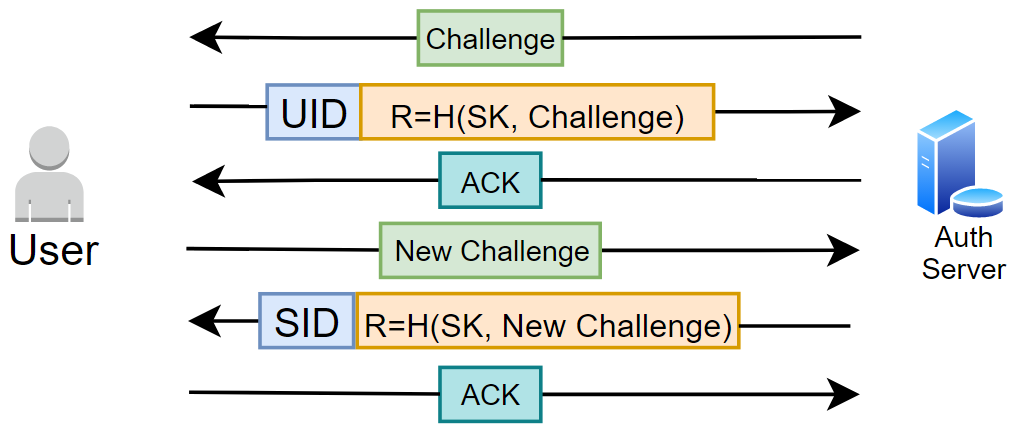
\includegraphics[width=0.9\textwidth]{image/chapmutual.png}
    \caption{Mutual Auth with Chap}
    \label{fig:chapmutual}
\end{figure}
\begin{remark}
L'idea di base non pone restrizioni sull'effettiva sequenza di messaggi che devono essere scambiati, questo pone un attaccante in posizione di vantaggio (\cref{fig:chapmutualatk}). Difatti, l'hacker potrebbe inoltrare al server la stessa challenge e lui dovrebbe rispondere con il suo nome e l'hash della challenge. A questo punto l'hacker si è mostrato legittimo per il server e può autenticare la sua identità digitale inoltrando la response precedente. 
\end{remark}
\begin{figure}[h]
    \centering
    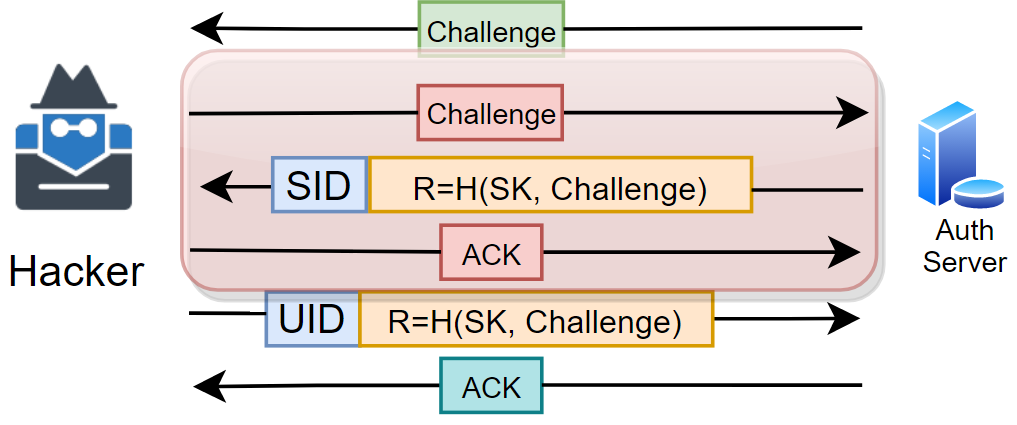
\includegraphics[width=0.9\textwidth]{image/chapmutualatk.png}
    \caption{Mutual Auth attack scheme}
    \label{fig:chapmutualatk}
\end{figure}
Lo schema precedente non è il solo attacco che diventa disponibile adesso, perché ora il sistema è soggetto al \textit{reflection attack}
\begin{definition}
[Reflection Attack]\label{def:reflectionatk}
L'attaccante è in grado di fingersi come access point. A questo punto può farsi inviare da un utente un messaggio con il quale può verificare la sua identità digitale. Lo schema è il seguente (\cref{fig:reflectionatk}): 
\begin{enumerate}
    \item A si finge access point ed invia una challenge $C_1$ ad U. 
    \item U invia la sua challenge $C_2$ (per autenticare l'altro end-point) e la sua response.\label{resp}
    \[(\text{UID}, H(K,C_1))\]
    \item A \textbf{ignora la response} e inoltre ad U la sua stessa challenge: (AID, $C_2$).
    \item U risponde di nuovo come al punto \ref{resp} con $C_2$ al posto di $C_1$
    \item A può autenticarsi, rispondendo con (AID, H(K,$C_2$))
\end{enumerate}
\end{definition}
\begin{figure}[h]
    \centering
    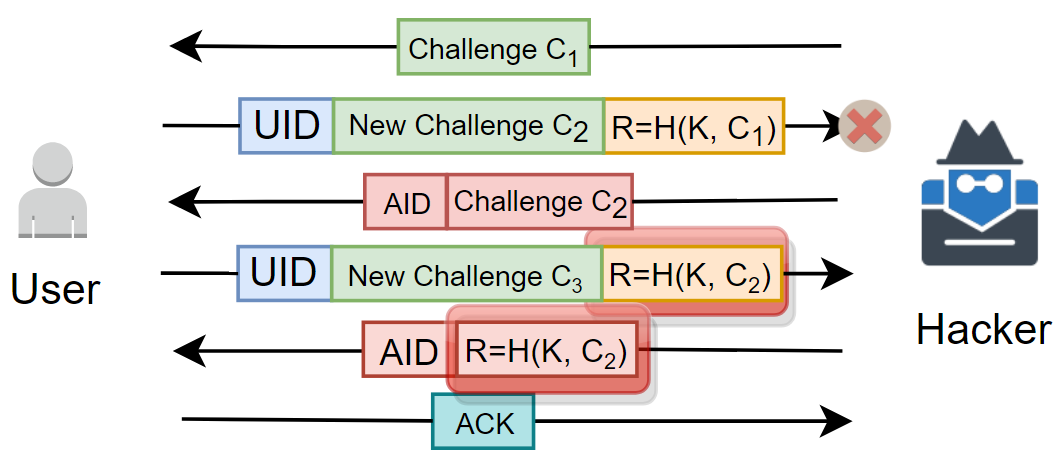
\includegraphics[width=0.9\textwidth]{image/reflectionatk.png}
    \caption{Reflection Attack in Mutual Auth}
    \label{fig:reflectionatk}
    \vspace{5pt}
\end{figure}
\subsection{Come prevenire Reflection Attacks?}
Un modo per impedire che le challenge siano riflesse, è tenere traccia della precedente challenge e dell'ordine con cui vengono inviate e calcolare l'hash di quella coppia come response. In questo modo anche osservando le challenge, un attaccante non potrà autenticarsi in quanto senza shared secret non potrà calcolare delle response valide. Lo schema, riportato in \cref{fig:reflectionavoid}, è:
\begin{enumerate}
    \item L'authenticator invia (SID, $C_1$).
    \item U genera $C_2$ ed invia (UID, $C_2$, H(K, $C_1$)). L'authenticator conosce l'ordine e può autenticare U.
    \item L'authenticator risponde con (SID, H(K, $C_1$, $C_2$)). U conosce l'ordine e può autenticare il server.
\end{enumerate}
\begin{figure}[ht]
    \centering
    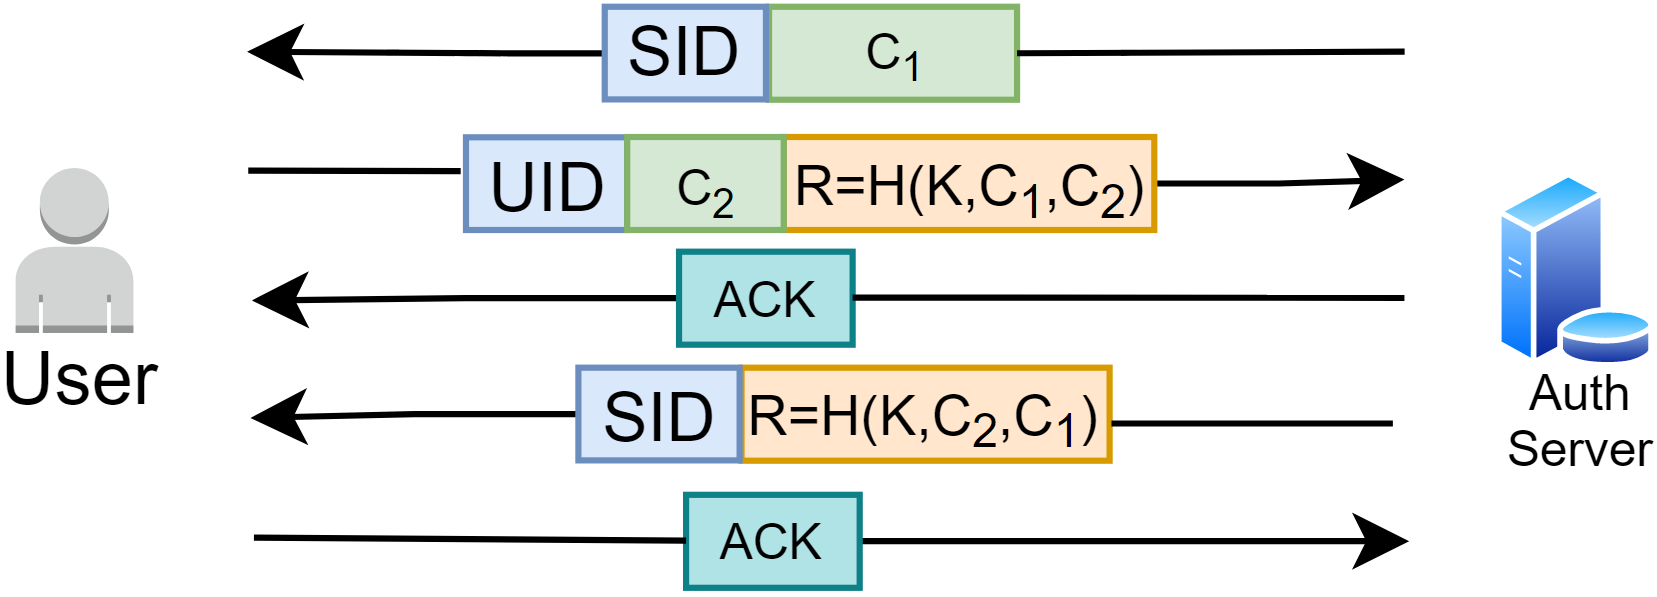
\includegraphics[width=0.8\textwidth]{image/reflectionavoid.png}
    \caption{Avoid Reflection Attack Scheme}
    \label{fig:reflectionavoid}
\end{figure}
\begin{corollary}[Lo scopo di un protocollo]
Mai usare un algoritmo per un obiettivo che non è quello per cui è stato pensato
\end{corollary}
La mutua autenticazione con CHAP è sbagliata di fondo, in quanto è un algoritmo pensato per essere \textit{"Single-Side authentication"}, mentre noi lo stiamo forzando a lavorare in un contesto \textit{"Dual-Side"}. Infatti, i reflection attacks ci sono ogni qualvolta usiamo uno stesso protocollo per autenticare due end-point. 
\begin{note}
Un protocollo di mutua autenticazione non può autenticare indipendentemente le due parti, in quanto espone vulnerabilità per il sistema. L'unico modo per eseguire il processo correttamente è quello di \textbf{legare insieme} le due challenge crittografandole in una unica response.
\end{note}

\chapter{Cellular Authentication}
Nelle reti cellulari passate\footnotemark (2G, 3G) gli aspetti di sicurezza vennero considerati in modo crescente ma non senza commettere errori e/o tralasciare aspetti fondamentali. Consideriamo qui aspetti e meccanismi di come un utente può autenticarsi in una rete cellulare e di come una stazione radio può confermare di essere valida. 
\footnotetext{Nella rete 1G la sicurezza non venne considerata affatto.}
\section{Rete 2G (GSM)}
In una rete GSM, le principali entità coinvolte in un processo di autenticazione sono le seguenti: 
\begin{itemize}
    \item \textbf{MS:} Mobile Sim (User). La sim contiene al suo interno una chiave segreta detta $K_i$\footnotemark, sconosciuta persino al dispositivo in cui la sim è inserita, così da poter non essere estratta.\footnotetext{Identity Key}
    \item \textbf{SN:} Serving Network (Visitor Location Register - VLR).
    \item \textbf{HN:} Home Network. E' l'unica a conoscere le chiavi $K_i$ degli utenti.
\end{itemize}
Quando un utente entra in rete, si avvia il seguente protocollo di autenticazione (\cref{fig:2gauth}): 
\begin{proposition}[2G Authentication]\label{prop:2gauth}
Assumiamo che l'utente abbia già notificato alla SN chi è e dove si trovi.
\begin{enumerate}
    \item La SN invia l'\textbf{IMSI}\footnotemark (identificatore dell'utente) e un \textbf{RAND} (sostanzialmente una challenge) alla \textbf{HN}.\footnotetext{\textsuperscript{\thefootnote}International Mobile Subscriber Identity}
    \item L'HN risponde con \textbf{SRES}\footnotemark (una response di tipo: H(RAND,$K_i$)) tramite un algoritmo $A3$ (una funzione hash) e un \textbf{encription key $K_C$} generata \textbf{dinamicamente} con l'algoritmo $A8$ a partire sempre da $K_i$ e \textbf{RAND}.\footnotetext{\textsuperscript{\thefootnote}Signed Result}
    \item La SN invia un'\textbf{authentication request} al MS inviando una nuova challenge \textbf{RAND} di 128bit.
    \item La MS crea una \textbf{authentication response} \textbf{SRES} da 32bit a partire dalla challenge di 128 e da $K_i$, tramite $A3$.
    \item La SN controlla se gli \textbf{SRES} corrispondono. In caso affermativo, consente l'accesso.
\end{enumerate}
\end{proposition}
Il punto di forza di questo protocollo di autenticazione è il concetto di \textit{\textbf{Key Derivation}}
\begin{definition}[Key Derivation]\label{def:keyderiv}
Concetto \textbf{fondamentale} con cui, a partire da una singola chiave che resta segreta per quasi\footnotemark ogni entità, è possibile generare delle nuove chiavi sempre diverse. 
\footnotetext{\textsuperscript{\thefootnote}Generalmente la chiave è codificata nell'hardware della scheda e salvata nel database dell'operatore.}
\end{definition}
\begin{figure}[ht]
    \centering
    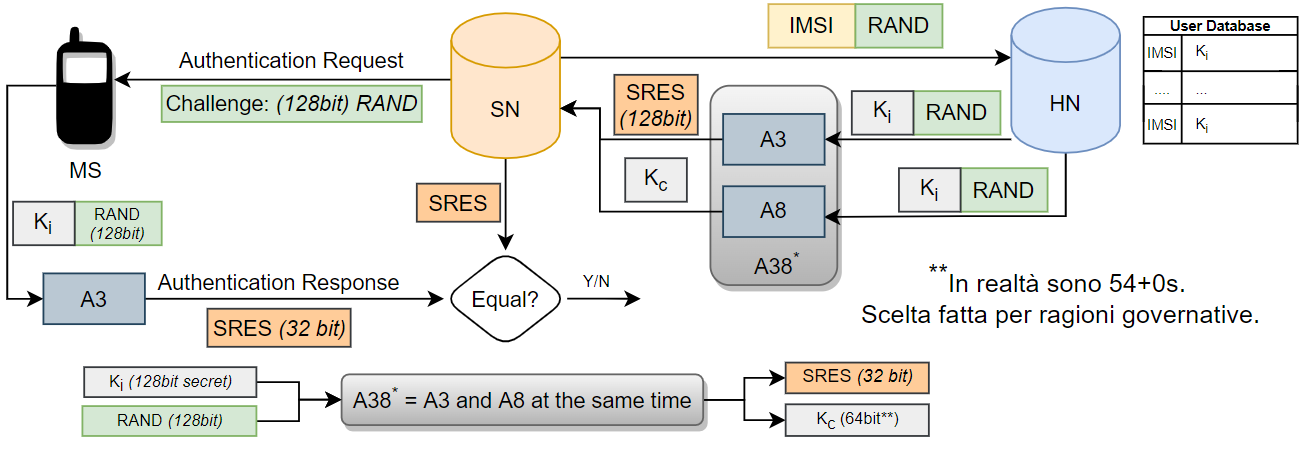
\includegraphics{image/2gauth.png}
    \caption{2G Authentication Scheme}
    \label{fig:2gauth}
\end{figure}
\begin{corollary}[Authentication Vector]\label{cor:authvect}
Tripletta di valori generata dalla Home Network per consentire l'autenticazione di un utente nella rete.
\begin{equation*}
    \text{AuthVect}=\{\text{RAND}, \text{SRES}, K_c\}
\end{equation*}
\end{corollary}
Poiché in uno scenario reale un utente può autenticarsi molte volte in un lasso di tempo abbastanza breve, tipicamente il processo di auth viene ottimizzato \textbf{inviando alla SN una sequenza di authentication vector}. In questo modo, per $N$ richieste di auth la SN sarà da subito in grado di autenticare un utente, senza dover avviare lo scambio di messaggi con la HN.\\
Inoltre, viene ridotta anche la frequenza con cui una SN e la HN comunicano tra loro, riducendo l'impatto del processo sul traffico generale.
\subsection{Vulnerabilità delle reti GSM}
Nelle reti GSM la vulnerabilità principale è data dal fatto che il protocollo è \textbf{unilaterale} verso l'utente:
\begin{note}
    \textbf{\textit{non abbiamo garanzie}}  sull'autenticità della service network/stazione radio base\footnotemark.
\end{note}
\begin{proposition}[Rogue BTS Attack]
I sistemi GSM non supportano \textbf{mutua autenticazione}, rendendo possibile la creazione di una fake BTS con la quale generare dizionari di utenti che provano a connettersi e, volendo, autenticarsi al posto loro.
\end{proposition}
\footnotetext{In inglese BTS: base transceiver station}
Una possibile soluzione è quella di spostare la responsabilità di generare la challange alla home network, così che il fornitore stesso del servizio cellulare possa controllare l'autenticazione. In questo modo vengono inibiti attacchi basati sulla non affidabilità della SN e/o del canale tra SN e HN.\\
Una seconda vulnerabilità è dovuta al fatto che gli algoritmi di cifratura e derivazione (rispettivamente $A3$ e $A8$) erano algoritmi proprietari e, teoricamente, ogni operatore avrebbe dovuto implementare il proprio. Questo approccio è definito in gergo come:
\begin{definition}[Security by Obscurity]
\label{def:secbyobsc}
Filosofia di sicurezza per la quale un sistema è protetto semplicemente perché mantiene dei segreti sugli algoritmi che implementa.
\end{definition}
Ai tempi di GSM, gli operatori si misero d'accordo per implementare l'algoritmo \textit{COMP128}, considerato sicuro proprio perché non reso pubblico. Tuttavia, negli anni successivi l'algoritmo trapelò e violato in breve tempo.\\
\begin{remark}
Mai affidarsi per la sicurezza di algoritmo al fatto che questo possa essere privato perché prima o poi questo verrà bucato. E' fondamentale, invece, affidarsi agli esperti di crittografia e mai implementare soluzioni "fatte in casa".
\end{remark}
\begin{note}
Riguardo alla dimensione effettiva del digest della chiave $K_c$, vennero standardizzati 64bit, suddivisi in 54 bit veramente sotto specifiche e una serie di zeri, in quanto a quei tempi nessuno era in grado di realizzare un attacco brute-force su una chiave di 54 bit (tantomeno su 64) se non i governi stessi, dotati di mezzi di calcolo più performanti.
\end{note}\pagebreak
\section{Rete 3G (UMTS)}
Nella rete UMTS l'autenticazione è bilaterale \textit{(Mutual Auth \cref{chap:mutualauth})} e garantisce che i parametri usati nel processo siano sempre nuovi, evitando il riutilizzo di chiavi. Lo schema è il seguente:
\begin{proposition}[3G Authentication - AKA: Authentication and Key Agreement]\label{prop:3gauth}
Assumiamo che l'utente abbia già notificato alla SN chi è e dove si trovi.
\begin{enumerate}
    \item La SN invia l'IMSI del MS all'HN.
    \item\label{authvect5} L'HN invia $N$ authentication-vectors (\cref{cor:authvect}) fatti da quintuple, contententi:
    \[\{\text{RAND, XRES, CK, IK, AUTN}\}\]
    \begin{itemize}
        \item \textbf{RAND:} Authentication Challenge.
        \item $\textbf{XRES}=f_2(K,\text{RAND})$\textbf{:} Risultato atteso dalla CHAP-like authentication.
        \item $\textbf{CK}=f_3(K,\text{RAND})$\textbf{:} Cipher Key.
        \item $\textbf{IK}=f_4(K,\text{RAND})$\textbf{:} Integrity Key.
        \item $\textbf{AK}=f_5(K,\text{RAND})$\textbf{:} Authentication Key. Usato per mutual-authentication.
    \end{itemize}
    \item La SN inoltra a MS un \textbf{RAND} ed un \textbf{Autentication Number} definito come:
    \[\text{AUTN}=\{\text{SQN$\oplus$AK, AMF, MAC-A}\}\]
    \begin{itemize}
        \item \textbf{SQN:} Sequence Number (48bit).
        \item \textbf{AMF:} Auth\&Key Management Field (16bit). Specifica quale algoritmo o chiave da usare se ci sono scelte disponibili, finestra di sync e altri parametri. Utile per il cosiddetto \textbf{In-Band Signaling}.
        \item $\textbf{MAC-A}=f_1(K,\text{SQN, AMF, RAND})$\textbf{:} Message Auth Code permette all'MS di autenticare la rete (64bit).
    \end{itemize}
    \item Per autenticare la rete, MS esegue i seguenti passi:
    \begin{enumerate}
        \item genera la \underline{SUA} \textbf{AK} a partire dall'\textbf{AUTN} ricevuto.
        \item verifica la \textbf{"freschezza"} dell'informazione calcolando \textbf{SQN}$\oplus$\textbf{AK}$=$\textbf{SQN'} tale che:
        \[SQN'\in\text{\{SQN-MS+1, SQN-MS+\textbf{tollerance}\}}\]
        Dove \textbf{SQN-MS} è il contatore interno del MS mentre la tolleranza è utile a fini di resync in caso di messaggi persi.
        \item Se MS ha ricevuto un nonce valido, procede a rigenerare il \textbf{MAC-A}, verificando che sia uguale a quello ricevuto in \textbf{AUTN}. Se l'esito è positivo, invia la \textbf{RES} alla SN e aggiorna il valore del proprio sequence number come \textbf{SQN-MS $=$ SQN}.
    \end{enumerate}
    \item La SN confronta \textbf{RES} ed \textbf{XRES}, autenticando MS in caso affermativo.
\end{enumerate}
\end{proposition}
\begin{note}
Gli algoritmi implementati all'interno della SIM sono $f_1,f_2,f_3,f_4.f_5$. Questi algoritmi sono \textbf{pubblici} e servono per derivare le chiavi necessarie all'autenticazione, tranne il primo che costituisce una funzione di criptaggio\footnotemark\, e il secondo che è sostanzialmente una funzione hash.
\footnotetext{$f_1$ è detta: \textbf{\textit{Actual Proof of Knowledge}} e certifica la conoscenza della chiave.}
\end{note}\pagebreak
\begin{remark}
E' interessante osservare come il protocollo di \textbf{mutua autenticazione} usato \textbf{per validare la rete} è sostanzialmente basato su \textbf{un singolo messaggio}, quando ci aspetteremmo un protocollo di tipo \textit{3-way handshake} (3 messaggi). Analogamente, il meccanismo di \textbf{autenticazione del MS rispetto alla SN avviene come nella rete 2G} (\cref{prop:2gauth}).
\end{remark}
\begin{note}
E' bene specificare che l'autenticazione della HN nei confronti della MS avviene tramite \textbf{sequence number (SQN)}, mantenuto in sincronizzazione tra le diverse parti della rete\footnotemark\, come \textbf{\textit{nonce implicita}}. Questo evita l'invio di un'ulteriore challenge da parte del MS alla HN.
\footnotetext{La Home Network mantiene il suo contatore nella variabile \textbf{SQN-HE}.}
\end{note}
\begin{corollary}[Il ruolo dell'Anonymity Key]
L'AK viene utilizzata per \textbf{oscurare/mascherare}\footnotemark il sequence number in una fase in cui il \textbf{servizio di confidenzialità} non è ancora attivo. Ciò permette di risolvere il \textbf{Location Privacy Problem}, per il quale un attaccante può essere in grado di \textbf{determinare gli spostamenti di un utente tracciando incrementi del sequence number nella rete}.
\footnotetext{\textsuperscript{\thefootnote}Tramite $\oplus$.}
\end{corollary}
\subsection{(Pochi) Dettagli su IMSI-Catcher Attack}
Nel processo di auth (sia 3G che 2G) abbiamo supposto che l'utente si autentifichi una singola volta e, pertanto, che l'IMSI \textbf{venga inviato una sola volta nella rete}.
In condizioni normali è vero che viene inviato solo una volta l'IMSI dell'utente
Ma in generale, se ci dovessero essere errori di connessione o di autenticazione, la rete non può escludere l'utente e deve esserci un modo di recuperare la connessione. In quel caso, l'IMSI può essere inviato nuovamente, e potrebbe essere individuato.\\
Per evitare che l'IMSI venga catturato, forzandone un invio ripetuto magari tramite una rogue-BSS che disconnette l'MS, il protocollo impone che dopo la prima connessione venga usato sempre un IMSI \textit{temporaneo}: \textbf{TMSI}. Tale valore varia ogni volta, rendendo di fatto impossibile tracciare l'utente.

% inserire fig su 3g auth
% inserire fig sqn mask
% inserire fig su schema reti cellulari wireless dopo esonero
\subsection{(Pochi) Dettagli su Rete 4G/5G (LTE)}
La rete 4G (LTE) sfrutta lo stesso principio di autenticazione della rete 3G (UMTS), mentre la rete 5G sfrutta meccanismi molto più simili alle reti wi-fi, in quanto si pone l'obiettivo di fondere le tecnologie ed unificare le reti. 
\begin{note}[Riguardo 5G]\\
Il meccanismo di \textbf{key-derivation} è migliorato. I moduli che dovrebbero garantire integrità in realtà non sono sempre implementati in quanto aggiungono molto carico di lavoro ed è stato fatto solo dal 4G in poi. Vi è inoltre una netta separazione per garantire protezione, detta \textbf{Security Edge Protecion} per separare la Serving Network dalla Home Network
\end{note}

\chapter{RADIUS}
In contesti reali dove le reti hanno una dimensione molto elevata, usare un sistema di autenticazione CHAP-like come visto fino ad ora è impensabile. Questo p erché esistono diversi modi di connettersi alla rete e quando i numeri sono grandi possiamo riscontrare tre problemi principali:
\begin{itemize}
    \item Se mantengo DB distribuiti ci sono tanti punti che possono essere attaccati.
    \item Quando viene cambiato il valore di una variabile (es. una password) bisogna propagare l'informazione a tutti i DB.
    \item C'è necessità di avere \textit{qualcuno} dotato di permessi di gestione (admin).
\end{itemize}
Per questo è stato sviluppato RADIUS, che sfrutta dei \textbf{server (logicamente) centralizzati}, mantenendo \textbf{1 server primario} più altri server secondari replicati.
\section{Funzionamento e Autenticazione}
\begin{definition}[RADIUS - Remote Authentication Dial In User Service]
Protocollo di tipo \textbf{AAA UDP-based}\footnotemark, che fornisce: 
\footnotetext{\textsuperscript{\thefootnote}Triple A}
\begin{itemize}
    \item \textbf{(Remote) Authentication:} certifica l'identità digitale di un utente, anche se questo non può connettersi alla stessa rete del server autenticante.
    \item \textbf{Authorization:} gestisce i \textbf{permessi} di \textbf{accesso} ai servizi degli utenti autenticati.\footnotemark
    \footnotetext{\textsuperscript{\thefootnote}ES: un set di canali di una pay-per-view che rientrano nell'abbonamento dell'utente.}
    \item \textbf{Accounting:} \textbf{tiene traccia} delle \textbf{azioni eseguite dagli utenti}\footnotemark
    \footnotetext{\textsuperscript{\thefootnote}ES: quando tempo passano su un servizio X o la spesa fatta per un bene Y.}
\end{itemize}
\end{definition}
\begin{figure}[h]
    \centering
    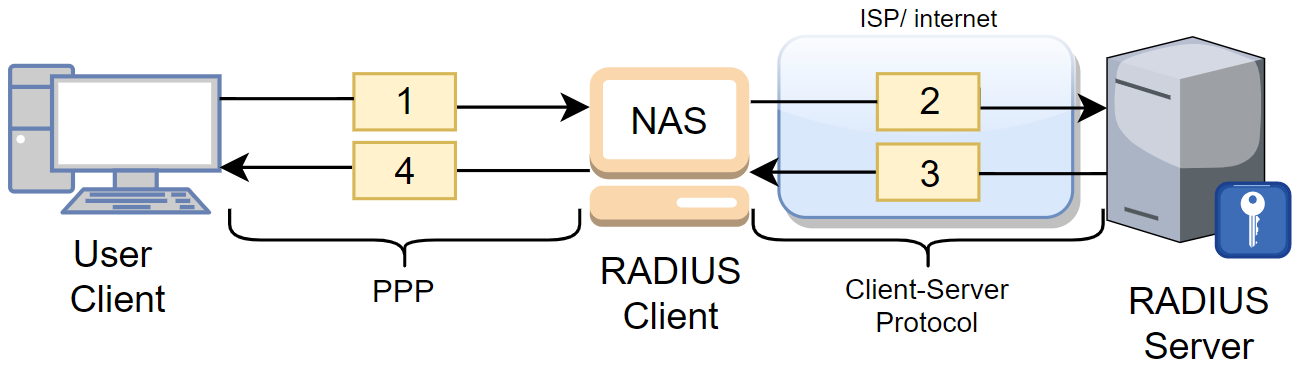
\includegraphics[width=0.8\textwidth]{image/radius.png}
    \caption{Main RADIUS components}
    \label{fig:radiusscheme}
\end{figure}\pagebreak
Le principali componenti del protocollo sono le seguenti:
\begin{definition}[RADIUS Entities]
\begin{itemize}
    \item \textbf{PPP} (Point to Point Protocol): Utilizzato per l'autenticazione tra il sistema dell'utente ed il \textbf{NAS/RAD client}. Generalmente si usano PAP o CHAP.
    \item \textbf{RADIUS Client/NAS} (Network Access Server): \textit{punto di accesso} che permette agli utenti di autenticarsi nella rete per sfruttarne i servizi. 
    \item \textbf{RADIUS Server:} \textbf{mantengono} le \textbf{credenziali degli utenti} in DB centralizzati ed erogano i servizi offerti dalla rete. I database sono di tre tipi:
    \begin{itemize}
        \item \textbf{Registered User Database:} per ogni utente si mantengono le credenziali e le modalità di autenticazione e gli attributi relativi al servizio di autorizzazione.
        \item \textbf{Client Database:} Mantiene le informazioni relative ai \textit{NAS} ammessi come radius client. 
        \item \textbf{Accounting Database:} Per ogni utente vengono mantenute informazioni relative al servizio di accounting.
    \end{itemize}
\end{itemize}
\end{definition}
Il processo di autenticazione avviene (nei minimi dettagli) nel seguente modo: 
\begin{proposition}[RADIUS Authentication \cref{fig:radiusscheme}]
\begin{enumerate}
    \item \textbf{PPP Request:} l'\textbf{utente invia} le proprie credenziali al \textbf{RAD client}.
    \item \textbf{RADIUS Request:} il NAS converte/include le credenziali ricevute in un \textbf{Messaggio di Richiesta}, che invia al \textbf{RAD Server}
    \item \textbf{RADIUS Response:} il \textbf{RAD Server} elabora la richiesta e produce un \textbf{Messaggio di Risposta}, che invia al \textbf{RAD client} che l'aveva contattato.
    \item \textbf{PPP Response:} il NAS notifica all'utente l'esito dell'autenticazione ricevuto dal server.
\end{enumerate}
\end{proposition}
\subsection{Servizio di Proxy}
Il protocollo RADIUS supporta connessioni remote, anche quando non possiamo connetterci direttamente alla rete desiderata. Difatti i RADIUS server svolgono la funzione di \textbf{Proxy Server} per altri RADIUS server \textbf{remoti}.
\begin{theorem}[Servizio di Proxy]
 Eseguono i servizi per conto di altri RADIUS server (es. facendo \textit{roaming} tra diversi ISP). Le funzionalità di proxy possono essere svolte sia in maniera trasparente che non, specificandolo nel contenuto del messaggio.
\end{theorem}\pagebreak
\section{Pacchetti RADIUS}
Come ogni protocollo, RADIUS impone una precisa specifica per il formato dei suoi messaggi:
\begin{figure}[h]
    \centering
    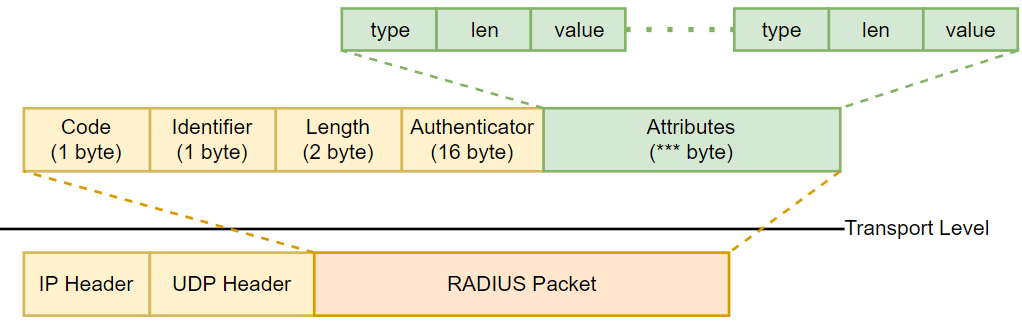
\includegraphics{image/radpack.png}
    \caption{RADIUS Packet Structure}
    \label{fig:radpack}
\end{figure}
\begin{itemize}
    \item \textbf{Code:} indica il \textbf{tipo} di \textbf{Pacchetto RADIUS}. I principali sono:
\end{itemize}
        \begin{definition}[Main Code Values]
        \begin{itemize}
            \item \textbf{Access-Request (1):} richiesta di autenticazione.
            \item \textbf{Access-Accept (2):} autenticazione avvenuta con successo.
            \item \textbf{Access-Reject (3):} autenticazione fallita/ rifiutata.
            \item \textbf{Accounting-Request (4):} richiesta di memorizzazione informazioni.
            \item \textbf{Accounting-Response (5):} risposta alla memorizzazione di informazioni.
            \item \textbf{Access-Challenge (11):} l'autenticazione richiede ulteriori messaggi.
        \end{itemize}
        \end{definition}
\begin{itemize}
    \item \textbf{ID:} specifica l'identificatore per l'autenticazione e serve a \textbf{legare} richiesta e risposta.
    \item \textbf{Length:} specifica la lunghezza del pacchetto, che è \textbf{sempre} compresa tra 20 e 4096 bytes.
    \item \textbf{Authenticator:} dipende dal tipo di pacchetto. Può essere:
    \begin{itemize}
        \item \textbf{Request:} \textbf{nonce} generata casualmente per il protocollo di autenticazione.
        \item \textbf{Response:} \textbf{digest MD5} per l'autenticazione del messaggio di risposta.
    \end{itemize}
    \item \textbf{Attributes:} lista di \textbf{campi} in formato \textbf{AVP} (Attribute Value Pair). Ogni campo è costituito da:
    \begin{itemize}
        \item \textbf{Type:} (1 byte) indica il tipo/significato del campo.
        \item \textbf{len:} lunghezza in byte del campo.
        \item \textbf{Value:} payload del campo.
    \end{itemize}
\end{itemize}
\begin{note}
Il campo attributes è un \textbf{extensible information field}.
\end{note}
\begin{definition}[Extensible Information Field]
Un campo è di tipo extensible information se il numero, il tipo e l'ordine delle informazioni contenute al suo interno può variare in base alle esigenze.
\end{definition}
\begin{remark}
Per costruzione non possiamo avere più di $2^8=256$ attributi differenti univocamente identificati a causa della dimensione del sottocampo \textbf{type}. In genere, un pacchetto di \textbf{Access-Request} contiene sempre i seguenti attributi:
\begin{itemize}
    \item \textbf{User-Name:} identificatore dell'utente.
    \item \textbf{User-Password:} password dell'utente, oscurata nel protocollo PPP-PAP.
    \item \textbf{Chap-Password:} challenge del protocollo PPP-CHAP, se utilizzato.
    \item \textbf{NAS-Identifier:} identificatore univoco del RADIUS client.
    \item \textbf{NAS-IP-Address:} indirizzo IP del RADIUS client.
    \item \textbf{NAS-Port:} porta UDP del RADIUS client.
\end{itemize}
\end{remark}

\section{Autenticazione in dettaglio}
Consideriamo il processo di autenticazione messo in atto dal RAD client e dal RAD server:
\begin{proposition}[Authentication Details]
\begin{enumerate}
    \item Il RAD client genera un \textbf{ID} per \textbf{identificare la richiesta} e una \textbf{nonce ReqAuth} per l'autenticazione. Mantiene la coppia \{\textbf{ID, ReqAuth}\} generata in un database locale ed invia una \textbf{RADIUS-Request}, contenente anche le credenziali di accesso ricevute tramite protocollo PPP dall'utente.
    \item Il RAD server genera una \textbf{RADIUS-Response}, composta da un digest prodotto tramite \textbf{MD5} secondo il seguente schema:
    \[\text{digest}=\text{MD5}(\text{Code||ID||Length||Auth||Attributes||S})\]
    \begin{itemize}
        \item \textbf{ID:} uguale per request e response.
        \item \textbf{Code, Length, Attributes:} specifiche del messaggio di risposta.
        \item \textbf{Auth:} nonce contenuta nel messaggio di richiesta e generata dal RAD Client.
        \item \textbf{S:} secret key condivisa tra RAD-client e RAD-server.
    \end{itemize}
    \item Il RAD-Client rigenera il digest utilizzando il suo DB per recuperare l'ReqAuth relativo all'ID ricevuto e verifica che sia uguale a quello ricevuto nella \textbf{RADIUS-Response}.
    \begin{itemize}
        \item In caso negativo, il RAD-Client comunica all'utente tramite protocollo PPP il fallimento dell'autenticazione. 
        \item In caso positivo, possiamo avere tre outcome diversi:
        \begin{enumerate}
            \item \textbf{response = Access-Accept:} viene comunicato all'utente tramite protocollo PPP l'avvenuta autenticazione e tutti i parametri di configurazione necessari.
            \item \textbf{response = Access-Reject:} le \textbf{credenziali di accesso} e/o degli \textbf{attributi nella richiesta} \textbf{non} sono \textbf{validi}. Viene comunicato all'utente il fallimento tramite protocollo PPP.
            \item \textbf{response = Access-Challenge:}Il RAD-Server ha bisogno di \textbf{ulteriori informazioni} per poter autenticare l'utente. Il \textbf{NAS} si occupa perciò di \textbf{recuperare} tali \textbf{informazioni} dall'utente ed invia una nuova \textbf{Access-Request.}
        \end{enumerate}
    \end{itemize}
\end{enumerate}
\end{proposition}
\begin{figure}[ht]
    \centering
    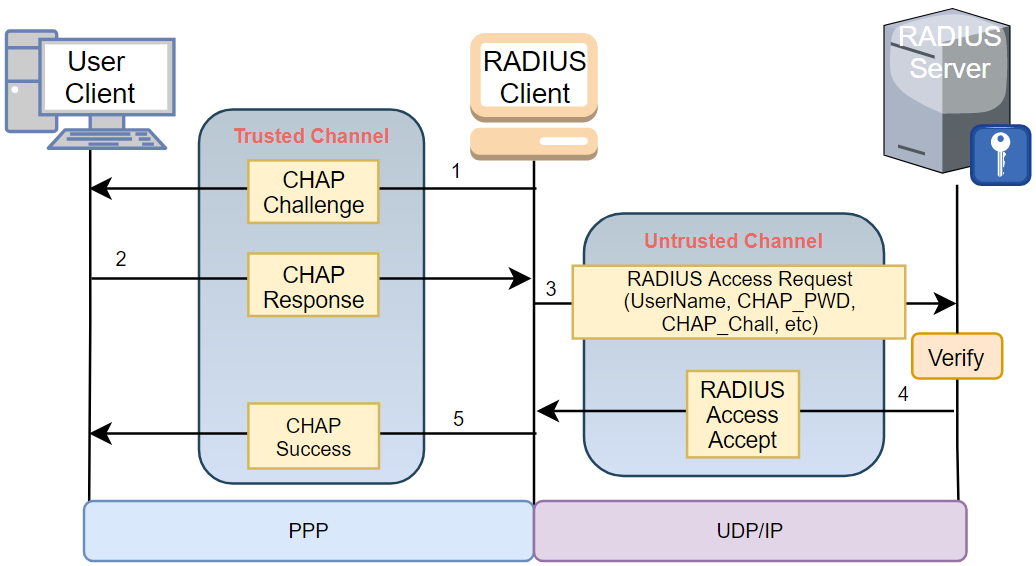
\includegraphics[width=0.85\textwidth]{image/chaprad.png}
    \caption{CHAP authentication in RADIUS}
    \label{fig:chaprad}
\end{figure}
\subsection{Challenge in PPP-CHAP}
Nel caso in cui PPP sia di tipo CHAP, la challenge per l'autenticazione CHAP tra utente e NAS viene gestita nel seguente modo:
\begin{definition}[PPP-CHAP]\label{def:chapradius}
\begin{enumerate}
    \item Il NAS genera la challenge per l'utente che vuole essere autenticato.
    \item L'utente genera ed invia ed invia la CHAP-response\footnotemark\, al RAD-client che la inoltrerà al RAD-Server insieme alla challenge.
    \item Il RAD-Server verifica la validità della coppia \{CHAP-challenge, CHAP-Response\} e di altri parametri tra cui l'ID, rigenerando la response tramite le credenziali in suo possesso e la challenge appena ricevuta.
\end{enumerate}
\footnotetext{\textsuperscript{\thefootnote}CHAP-Response $=$ H(user-PWD, CHAP-Challenge)}
\end{definition}
\section{Servizi di Sicurezza}
I servizi di sicurezza offerti dal protocollo sono: 
\begin{theorem}[Servizio di Sicurezza]
 \begin{itemize}
     \item \textbf{Autenticazione delle RAD Response:} i messaggi di risposta sono autenticati con un meccanismo \textbf{CHAP-Like}\footnotemark, basato sulla conoscenza di un segreto condiviso e sull'uso di una crypto-hash function.
     \item \textbf{Confidenzialità sulle PWD degli Utenti:} le password degli utenti sono criptate prima dell'autenticazione.
 \end{itemize}
 \footnotetext{\textsuperscript{\thefootnote}Viene evitato l'invio in chiaro delle password. In altre parole non c'è trasmissione di segreti.}
\end{theorem}
\subsection{Vulnerabilità nella Sicurezza}
I servizi di sicurezza offerti da RADIUS non sono perfetti, né lato autenticazione né su lato confidenzialità. Vediamo perché:
\begin{corollary}[Errori di Autenticazione]
\begin{itemize}
    \item Soltanto la \textbf{RADIUS Response} viene autenticata, lasciando spazio ad attacchi.
    \item Uso \textbf{forzato} della funzione hash \textbf{MD5} (non HMAC \cref{def:hmac})
    \item uso di \textbf{chiavi simmetriche} a \textbf{bassa entropia}.
\end{itemize}
\end{corollary}
\begin{corollary}
[Errori di Confidenzialità]
\begin{itemize}
    \item Meccanismi \textbf{personalizzati} per la cripatazione delle password.
    \item \textcolor{red}{\textbf{Riutilizzo della chiave di auth per fare encryption}}.
    \item Trasmissione in chiaro dei messaggi protocollari.
\end{itemize}
\end{corollary}
Osserviamo preliminarmente che la trasmissione in chiaro dei messaggi di request e response lascia spazio all'intercettazione di tali messaggi e, soprattutto, ad un eventuale modifica nel caso della request in quanto non autenticata.\\
Vediamo nel dettaglio cosa implicano queste debolezze:
\begin{proposition}[RADIUS Request Non Autenticata]
\begin{itemize}
    \item \textbf{Vulnerabilità a MITM:} data la mancanza di cifratura sul canale, i messaggi di request/response possono essere creati.
    \item \textbf{Payload Replay Attack:} Attacco su due fronti che permette di autenticarsi con l'identità dell'utente vittima.
    \begin{enumerate}
        \item Supponiamo di posizionarci tra il RAD-client e il RAD-server e di poter osservare un'autenticazione valida dell'utente, \textbf{salvando CHAP-Chappenge e CHAP-Response}. 
        \item L'attaccante avvia una nuova autenticazione a nome della vittima, utilizzando una password fasulla. Poiché il NAS non fa controllo ed inoltra la request verso il RAD-server, l'attaccante può intercettarla e sostituendo \textbf{CHAP-challenge} e \textbf{CHAP-response} precedentemente memorizzate \textbf{(coppia valida)} viene visto come utente legittimo.
    \end{enumerate}
\end{itemize}
\end{proposition}
\begin{theorem}[Soluzione con Message Authentication Extension Protocol]
Più che un protocollo vero e proprio è un container che specifica come un pacchetto di auth dovrebbe essere fatto. 
Tecnica utile per rendere il protocollo resistente ad attacchi MITM. Il funzionamento prevede l'\textbf{aggiunta} di un \textbf{nuovo attributo} nella Access-Request per il controllo dell'integrità.
\end{theorem}\pagebreak
Si hanno così due campi di autenticazione:
\begin{itemize}
    \item Uno nell'\textbf{header RADIUS}, costituito dalla nonce a 16byte per la richiesta di autenticazione.
    \item Uno negli \textbf{attributi}: MAC per il controllo di integrità della request calcolato come
    \[\text{MAC}=\text{HMAC-MD5(Code||ID||Length||Auth||Attributes||S)}\]
    Dove il valore dell'attributo \textbf{Authenticator} è zero in quanto lo si sta calcolando e verrà poi rimpiazzato
\end{itemize}
\subsection{Confidenzialità della password in PPP-PAP}
Nel caso in cui il protocollo PPP sia di tipo PAP, la password dell'utente nella RAD-Request viene criptata utilizzando una nonce data dall'\textbf{ReqAuth} e la chiave segreta \textbf{S}, così da non rivelarla ad eventuali attaccanti in ascolto. Il processo di cifratura delle passwrod è il seguente: 
\begin{definition}[PWD Encryption in RADIUS]
\begin{enumerate}
    \item Data la password si effettua un padding fino a 16 byte, questa è la dimensione del blocco.
    \item Si calcola la nonce di ReqAuth e si esegue MD5(S||ReqAuth). 
    \item La password prima di essere spedita viene cifrata calcolando 
    \[\text{PWD}\oplus\text{MD5(S||ReqAuth)}\]
\end{enumerate}
Se la password è più lunga di 16 byte, viene suddivisa in blocchi da 16 e l'ultimo blocco riempito con un padding. In quel caso, eseguiamo:
\begin{algorithmic}
\ForAll{$\text{PWD}_{\text{blk}}$}
\State $\text{PWD}_{\text{enc}}=\text{PWD}_{\text{blk}}\oplus\text{MD5(S||ReqAuth)}$
\EndFor
\end{algorithmic}
\end{definition}
\pagebreak
\begin{proposition}[Bassa entropia delle chiavi]
La bassa entropia è dovuta al basso numero di caratteri coinvolti nelle chiavi (viene usato il set ASCII). Inoltre, in molti casi, \textbf{una sola password è utilizzata per tutta la rete dell'ISP}. Gli attacchi possibili sono due:
\begin{itemize}
    \item \textbf{Dictionary Attack alla chiave segreta S in PPP-PAP:} E' possibile creare un dizionario di coppie \textbf{\{ReqAuth, MD5(S, ReqAuth)\}} ascoltando i messaggi di Access-Request. Poiché MD5 posiziona il segreto alla fine (\cref{sub:secretpos}), è possibile precalcolare come blocco singolo la prima parte del messaggio e fare bruteforce diventa facile.\\
    \begin{remark}
    In realtà non c'è neanche bisogno della coppia: Inviando una coppia \{(user-ID, user-PWD)\} arbitraria, il NAS può agire come fosse un oracolo in un attacco CPA. Infatti intercettando l'Access-Request inviata, possiamo fare ottenere un digest MD5 valido calcolando:
    \[\text{MD5(S, ReqAuth)}=\text{user-PWD attribute}\oplus\text{password}\]
    E adesso possiamo cifrare una password qualsiasi.
    \end{remark}
    \item \textbf{Attacco alle pwd degli utenti in PPP-PAP:} L'attaccante invia un user ID questa volta valido e una password arbitraria da 16 byte. Intercettando i messaggi di Access-Request possiamo produrre un digest MD5 valido calcolando:
    \[\text{MD5(S, ReqAuth)}=\text{user-PWD attribute}\oplus\text{password}\]
    Adesso l'attaccante può cifrare una password qualsiasi.
\end{itemize}
\end{proposition}
\begin{note}[Dictionary Attack to Shared Secret Details]\\
L'attacco bruteforce è possibile solo con pwd inferiori a 16byte. In particolare, il NAS stesso può essere usato come un oracle in un attacco CPA. Intercettando i messaggi di Access-Request otteniamo la user-password attribute (16 bytes) e il Request Authenticator (16 bytes). Facendo uno xor tra la password cifrata e quella in chiaro otteniamo il digest dell'MD5.
\end{note}
\begin{note}[User-PWD Attack Details]\\
Anche questo attacco funziona con password di 16 bytes. Una volta ottenuto il digest valido possiamo bypassare tutte le limitazioni imposte lato client, come il numero di tentativi valido di autenticazione al RADIUS server.
\end{note}
\begin{figure}[h]
    \centering
    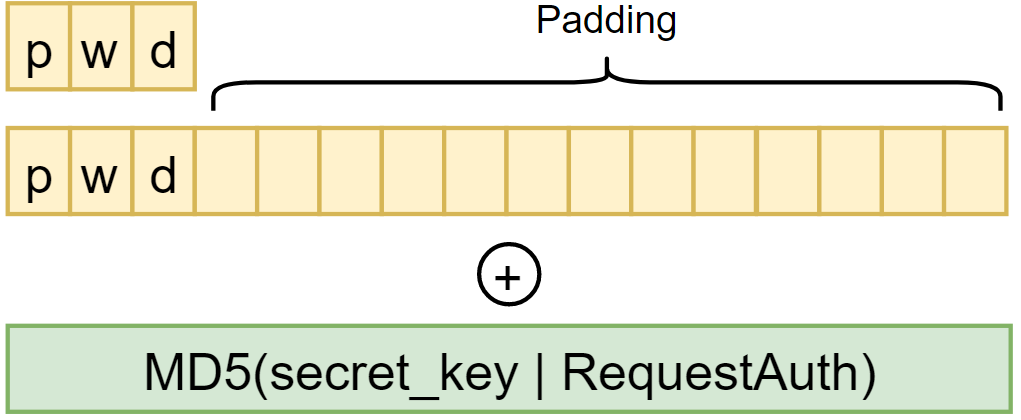
\includegraphics[width=0.5\textwidth]{image/radpwdenc.png}
    \caption{Password Encryption in RADIUS with PPP-PAP}
    \label{fig:radpwdenc}
\end{figure}
\subsection{Cattiva gestione dei PRNG}
Un'ulteriore errore commesso da RADIUS è una scarsa implementazione degli algoritmi di PRNG per la generazione delle nonce di ReqAuth, tipicamente non crypto-functions con \textbf{ciclo breve} (alta probabilità di collisione) e \textbf{alta predicibilità}. Questo significa che l'ipotesi di unicità della nonce viene meno e può permettere ad un attaccante di autenticarsi calcolando il valore della prossima nonce.\\
Ci sono 3 attacchi possibili che possono essere fatti:
\begin{itemize}
    \item \textbf{Birthday Attack:} Consideriamo un PRNG con ciclo di $2^n$ e al più $2^n$ valori differenti. Per il \textbf{paradosso del compleanno} \cref{eq:birthdayparadox} un valore si ripete con \textbf{probabilità del 50\%} con $2^\frac{n}{2}$ autenticazioni. Inoltre, alcune implementazioni potrebbero \textbf{usare più volte uno stesso PRNG} per generare una sola nonce, riducendo il ciclo di generazione.
    \item \textbf{Replay Attack:} L'attaccante può generare un dizionario \textbf{\{ID, AUTH, MD5\}} osservando coppie valide di \textbf{Access-Request/Access-Response} per effettuare un replay attack nel momento in cui il NAS genera una ReqAuth ripetuto. A quel punto è possibile autenticare/autorizzare un qualsiasi utente senza un pwd valida.\\
    L'ID può essere ricalcolato con brute-force in quanto costituito da un solo byte.
    \item \textbf{Attacco alle PWD degli utenti (se PPP-PAP):} Osservando le \textbf{Access-Request} l'attaccante genera un dizionario di \textbf{\{ReqAuth, PW-enc\}}. Se una nonce si ripete, è possibile ottenere informazioni sulle password degli utenti calcolando:
    \[\text{PW1}_{enc}\oplus\text{PW2}_{enc}=(\text{PW1}\oplus\text{MD5(S, ReqAuth)})\oplus(\text{PW2}\oplus\text{MD5(S, ReqAuth)})=\text{PW1}\oplus\text{PW2}\]
    Una volta ottenuto lo xor delle due passowrd in chiaro di due utenti bersaglio, poiché le dimensioni sono note e con buona probabilità di lunghezza differente, otteniamo in chiaro la parte finale della password più lunga e analizzando il risultato è possibile calcolare il risultato. Inoltre, è possibile velocizzare la generazione del dizionario effettuando delle Access-Request con password casuali (magari prese da un db online), consumando generazioni del PRNG.
\end{itemize}
\pagebreak
\section{DIAMETER}
RADIUS al giorno d'oggi è meno utilizzato di una volta in quanto presenta delle limitazioni importanti. In particolare:
\begin{itemize}
    \item \textbf{Scalabilità/Efficienza:} RADIUS supporta in maniera efficiente solo un numero ridotto di utenti. Questo è dovuto all'uso di UDP come protocollo di trasferimento, che implica un forte problema di packet loss nei casi di picchi di utenza.
    \item \textbf{Estensibilità:} il modo con cui gli attributi erano codificati imponeva limiti sulle nuove tecnologie e non era sufficiente a supportare possibili sviluppi futuri.
    \item \textbf{Interoperabilità:} non standardizzata e realizzata tramite soluzioni proprietarie (ogni venditore ha la sua soluzione).
\end{itemize}
DIAMETER è un'evoluzione di RADIUS, retrocompatibile e che risolve i le limitazioni analizzate prima. L'ottica con cui è sviluppato è simile alla logica "object-oriented": Viene definita una classe di \textbf{AAA Transport Profile} che specifica il tipo di livello di trasporto da usare (STCP/TCP-based) e una \textbf{base-class} DIAMETER più una serie di classi derivate per svariati tipi di servizi, tutte figlie della base-class.
\begin{note}
La DIAMETER Base Protocol è, più che un protocollo AAA, un protocollo di scambio di messaggi. 
\end{note}
\begin{figure}[h]
    \centering
    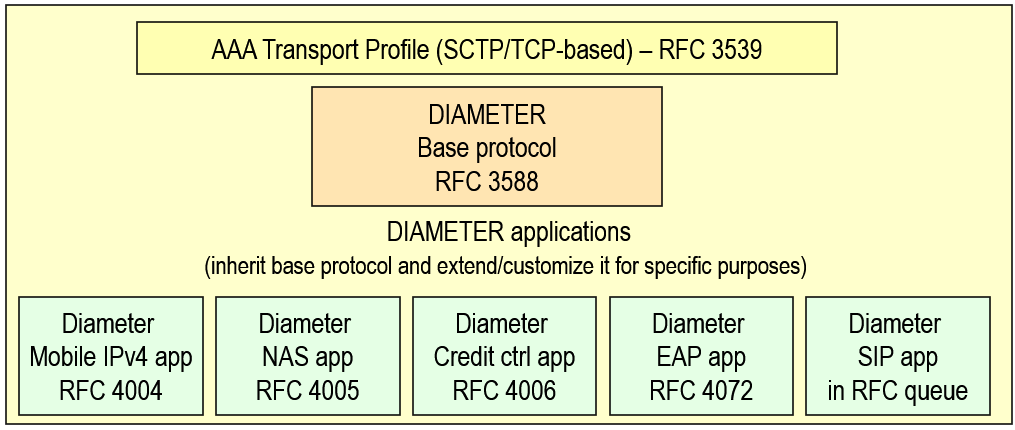
\includegraphics{image/diameter.png}
    \caption{DIAMETER Structure}
    \label{fig:diameter}
\end{figure}
\subsection{Feature Principali in DIAMETER}
\begin{proposition}[Trasporto Affidabile dei pacchetti]
 Utilizzo di \textbf{STCP/TCP} per il trasferimento affidabile dei pacchetti, instaurando connessioni persistenti tra client e server.
\end{proposition}
\begin{note}
    L'affidabilità è fondamentale per avere un accounting efficiente.
\end{note}
\begin{proposition}[Gestione degli Errori/Guasti standardizzata]
 L'error-control è demandato al livello applicativo. Inoltre, vengono implementate le seguenti funzionalità:
    \begin{itemize}
        \item \textbf{Rilevazione Duplicati:} vengono rilevati e scartati messaggi doppi.
        \item \textbf{Watchdog:} periodicamente vengono inviati dei pacchetti per conoscere lo stato dei vicini.
    \end{itemize}
\end{proposition}
\begin{note}
    In RADIUS la gestione degli errori dipende dall'implementazione
\end{note}
\begin{proposition}[Miglior Supporto all'Estensibilità]
il formato dei pacchetti è \textbf{modificato} e \textbf{ampliato}, per supportare più funzionalità. Tra i servizi implementati troviamo: 
    \begin{itemize}
         \item \textbf{Rilevazione Duplicati:} per ogni pacchetto vi è un ID.
        \item \textbf{Negoziazione:} è previsto un flag per specificare il comportamento che il destinatario deve attuare alla ricezione di parametri non supportati. 
    \end{itemize}
\end{proposition}
\begin{remark}
    RADIUS non supporta la rilevazione di duplicati né capacità di negoziazione dei parametri. Questo significa che il sistema non sa come rispondere ad un pacchetto con parametro non supportato.
\end{remark}
\begin{proposition}[Scoperta dei peers, configurazione e rilevamento capacità]
I \textbf{sistemi} DIAMETER \textbf{vicini} (peers) vengono \textbf{configurati} tramite \textbf{meccanismi automatici} accordandosi sulla versione del protocollo, sui meccanismi di sicurezza da usare e le applicazioni supportate.
\end{proposition}
\begin{proposition}[Supporto di Messaggi "Spontanei" da Server a Client]
Il server può inviare autonomamente dei messaggi al client al fine di supportare:
    \begin{itemize}
        \item \textbf{Disconnessioni volontarie} da parte del server.
        \item \textbf{Comunicazione di Errori/Fallimenti} al client.
        \item \textbf{Supportare} la \textbf{ri-autenticazione/ri-autorizzazione},
    \end{itemize}
\end{proposition}
    \begin{note}
    RADIUS supporta solo lo schema client-server, dove solo il primo avvia la comunicazione.
    \end{note}
\begin{proposition}[Gestione delle Entità Intermedie]
Viene specificata esplicitamente l'esistenza di diversi tipi di agenti, come \textbf{proxies, redirects, relay}. Inoltre, viene fatta distinzione tra:
    \begin{itemize}
        \item \textbf{Hop-By-Hop:} comunicazioni tra nodi intermedi.
        \item \textbf{End-To-End:} comunicazione tra nodi estremi, ovvero tra DIAMETER client e DIAMETER server.
    \end{itemize}
\end{proposition}
\begin{note}
    In RADIUS esiste solo hop-by-hop e non vengono specificate entità intermedie.
\end{note}
\subsection{Pacchetti DIAMETER}
I pacchetti DIAMETER possiedono il seguente formato:
\begin{itemize}
    \item \textbf{Header} [20 byte]: intestazione del messaggio
\end{itemize}
\begin{definition}[Header Structure]
\begin{itemize}
    \item \textbf{Version}[1byte]: versione del protocollo.
    \item \textbf{Message Length}[3 byte]: lunghezza del messaggio.
    \item \textbf{Flags}[1 byte]: flag per specificare la funzionalità
    \begin{itemize}
        \item \textbf{P (Request):} indica se il messaggio è una \textbf{richiesta}(1) o una \textbf{risposta} (0).
        \item \textbf{P (proxiable):} Indica se è possibile effettuare \textbf{proxying} del messaggio.
        \item \textbf{E (Error):} indica se è un messaggio di \textbf{errore}.
        \item \textbf{T:} indica se il messaggio è stato ritrasmesso.
    \end{itemize}
    \item \textbf{Command Code}[3 byte]: indica il \textbf{tipo} di messaggio.
    \item \textbf{Application ID}[4byte]: indica l'applicazione di appartenenza.
    \item \textbf{Hop-By-Hop ID}[4 byte]: identifica il canale tra due nodi intermedi della comunicazione.
    \item \textbf{End-To-End ID}[4 byte]: identifica gli estremi della comunicazione.
\end{itemize}
\end{definition}
\begin{figure}[h]
    \centering
    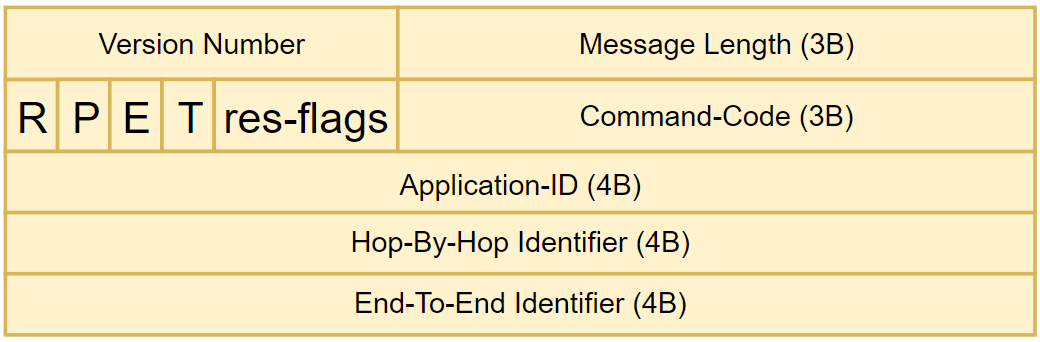
\includegraphics[width=0.7\textwidth]{image/diamheader.png}
    \caption{DIAMETER Header}
    \label{fig:diamheader}
\end{figure}
\begin{itemize}
    \item Attributes: Lista dei campi in formato \textbf{AVP}\footnotemark\,.
\end{itemize}
\begin{definition}[AVP format]
\begin{itemize}
    \item \textbf{AVP Code}[4 byte]: indica il tipo di campo.
    \item \textbf{Flags}[1 byte]: flag per indicare funzionalità.
    \begin{itemize}
        \item \textbf{V (Vendor):} indica se è presente il Vendor ID nell'AVP.
        \item \textbf{M (Mandatory):} indica se l'AVP deve essere \textbf{obbligatoriamente supportato}.
        \item \textbf{P (Protected):} Indica se è necessaria la criptazione end-to-end.
    \end{itemize}
    \item \textbf{AVP Length}[3 byte]: lunghezza del campo.
    \item \textbf{Vendor ID}[4 byte]: presente se \textbf{V=1}. Sostituisce il ruolo dell'AVP Code.
    \item \textbf{Data:} payload del campo.
\end{itemize}
\end{definition}
\footnotetext{Attribute Value Pair}
\begin{figure}[ht]
    \centering
    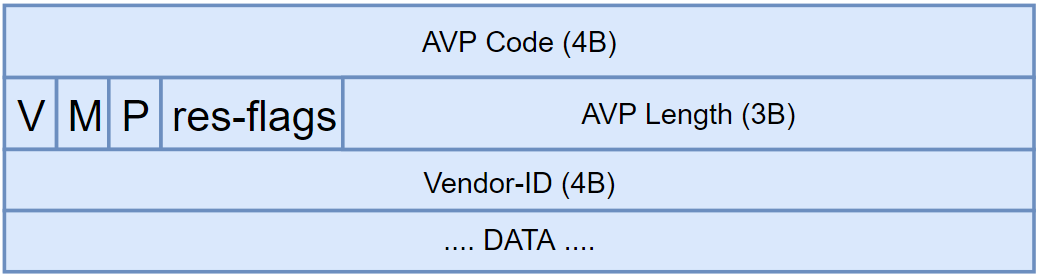
\includegraphics[width=0.7\textwidth]{image/avpheader.png}
    \caption{AVP Header}
    \label{fig:avpheader}
\end{figure}\pagebreak
\begin{note}\textbf{[Mandatory Flag-Bit]}\\
Questo flag negli AVP permette di realizzare il cosiddetto \textbf{Incremental Deployment}, ovvero la possibilità di implementare aggiornamenti nel sistema continuando a \textbf{supportare meccanismi preesistenti}. In particolare, per ogni AVP, ovvero per ogni attributo, viene applicata la seguente logica:
\begin{itemize}
    \item [\textbf{M=1}] il campo AVP è \textbf{necessario} alla funzionalità traspostata nel messaggio Nel caso in cui \textbf{non} venga \textbf{compreso/supportato} dal \textbf{ricevente}, quest'ultmo avvia una \textbf{negoziazione} con il \textbf{mittente} per determinare una configurazione supportata da entrambi.
    \item [\textbf{M=0}] il campo AVP è \textbf{non necessario} alla funzionalità trasportata dal messaggio. Nel caso in cui \textbf{non} venga \textbf{compreso/supportato} dal ricevente, viene silenziosamente \textbf{scartato}.
\end{itemize}
\end{note}
\subsection{Agenti Intermedi}
DIAMETER prevede e supporta i seguenti tipi di \textbf{agenti intermedi}:
\begin{definition}[Relay Agent]
Accetta richieste e le \textbf{instrada al DIAMETER server} appropriato basandosi sul contenuto della richiesta stessa e usando una specifica tabella di instradamento.
\end{definition}

\begin{definition}[Proxy Agent]
Effettua le stesse operazioni del relay agent ma può modificare i messaggi che instrada.
\end{definition}

\begin{definition}[Redirect Agent]
 Permette di effettuare la \textbf{separazione} del \textbf{control-plane} dal \textbf{data-plane} cooperando con un relay agent. In particolare, si occupa di \textbf{prendere} le \textbf{decisioni} di \textbf{instradamento} al posto del relay agent.\\
 Tali decisioni verranno comunicate al relay tramite \textbf{notifiche} di \textbf{direzione}, il quale applicherà l'instradamento deciso.\\
 Ciò è utile nel caso in cui si vogliano \textbf{centralizzare} tutte le \textbf{scelte} di \textbf{instradamento} in un'unica entità, così da semplificare la gestione della rete.
\end{definition}

\begin{figure}[ht]
    \centering
    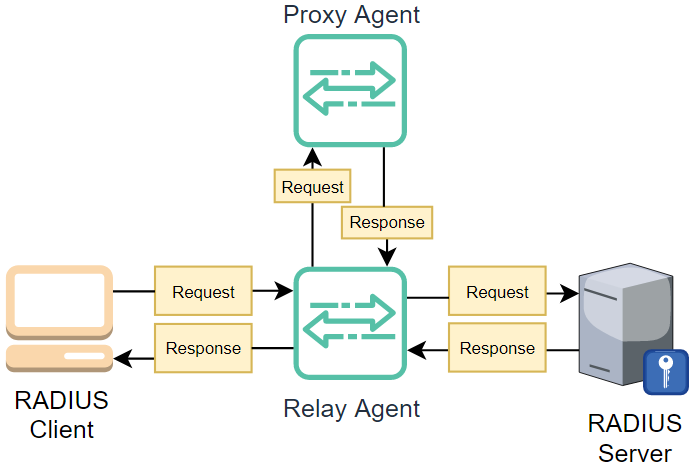
\includegraphics[width=0.8\textwidth]{image/relayagent.png}
    \caption{Relay Agent}
    \label{fig:relayagent}
\end{figure}
\chapter{Block Ciphers}\label{chap:blkcipher}
L'obiettivo dei Block Ciphers è quello di fornire dei meccanismi più "generali" di cifratura rispetto ai substitution ciphers. Lo schema base di un cifratore a blocchi è il seguente:
\begin{figure}[h]
    \centering
    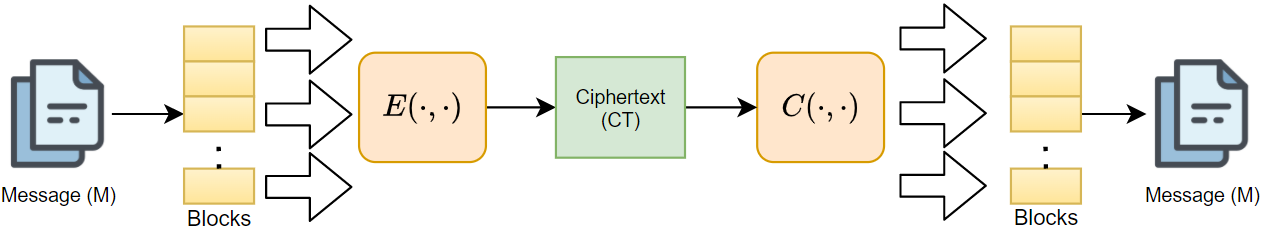
\includegraphics{image/blockcipher.png}
    \caption{Block Cipher Scheme}
    \label{fig:blkcipher}
\end{figure}
\section{Funzionamento di Base}
L'idea alla base dei block cipher è quella di dividere il messaggio in blocchi di dimensione specifica che vengono poi cifrati con una chiave $K$. Inoltre, ogni algoritmo di questo tipo \textbf{deve} implementare una logica di \textbf{pseudo-random permutation}, basata sulla dimensione della chiave usata. Tale permutazione deve avere le seguenti proprietà:
\begin{property}[Pseudo Random Permutation]
\begin{itemize}
    \item \textbf{Biettiva e Reversibile:} dato un input abbiamo un solo output e dato un output dobbiamo poter risalire all'input.
    \item \textbf{Associazione Pseudo-Random:} l'associazione fra i caratteri di partenza con quelli di arrivo deve essere una permutazione casuale. 
\end{itemize}
\end{property}
Il problema di avere una funzione biettiva, è che se un messaggio una volta diviso in blocchi presentasse due blocchi uguali, avremmo uno stesso testo cifrato per quei due blocchi. Stesso discorso se cifriamo due volte lo stesso messaggio.\\
Questo è il funzionamento della modalità \textbf{ECB} \textit{(Electronic Code Book)} , che non va mai usato perché \textbf{perdiamo semantic security}.\\
\begin{remark}Supponiamo di avere una chiave di dimensione $n=3$bit. L'insieme di tutti i plaintext possibili è di dimensione 8, quindi le permutazioni possibili sono $2^3!=8!=40320$.\\
Se consideriamo \textit{AES} la dimensione della chiave è di 128 bit, quindi il numero di permutazioni è incredibilmente elevato. 
\end{remark}
\begin{note}In realtà in \textit{AES} le permutazioni sono di meno, perché vengono richieste delle proprietà aggiuntive.
\end{note}
Una possibile soluzione per ovviare al problema descritto sopra è ovviamente quello di inserire degli \textit{initialization vectors} per nascondere il plaintext al momento dell'applicazione della funzione di \textbf{PRP} \textit{(pseudorandom permutation)} secondo il seguente schema:
\pagebreak
\begin{figure}[ht]
    \centering
    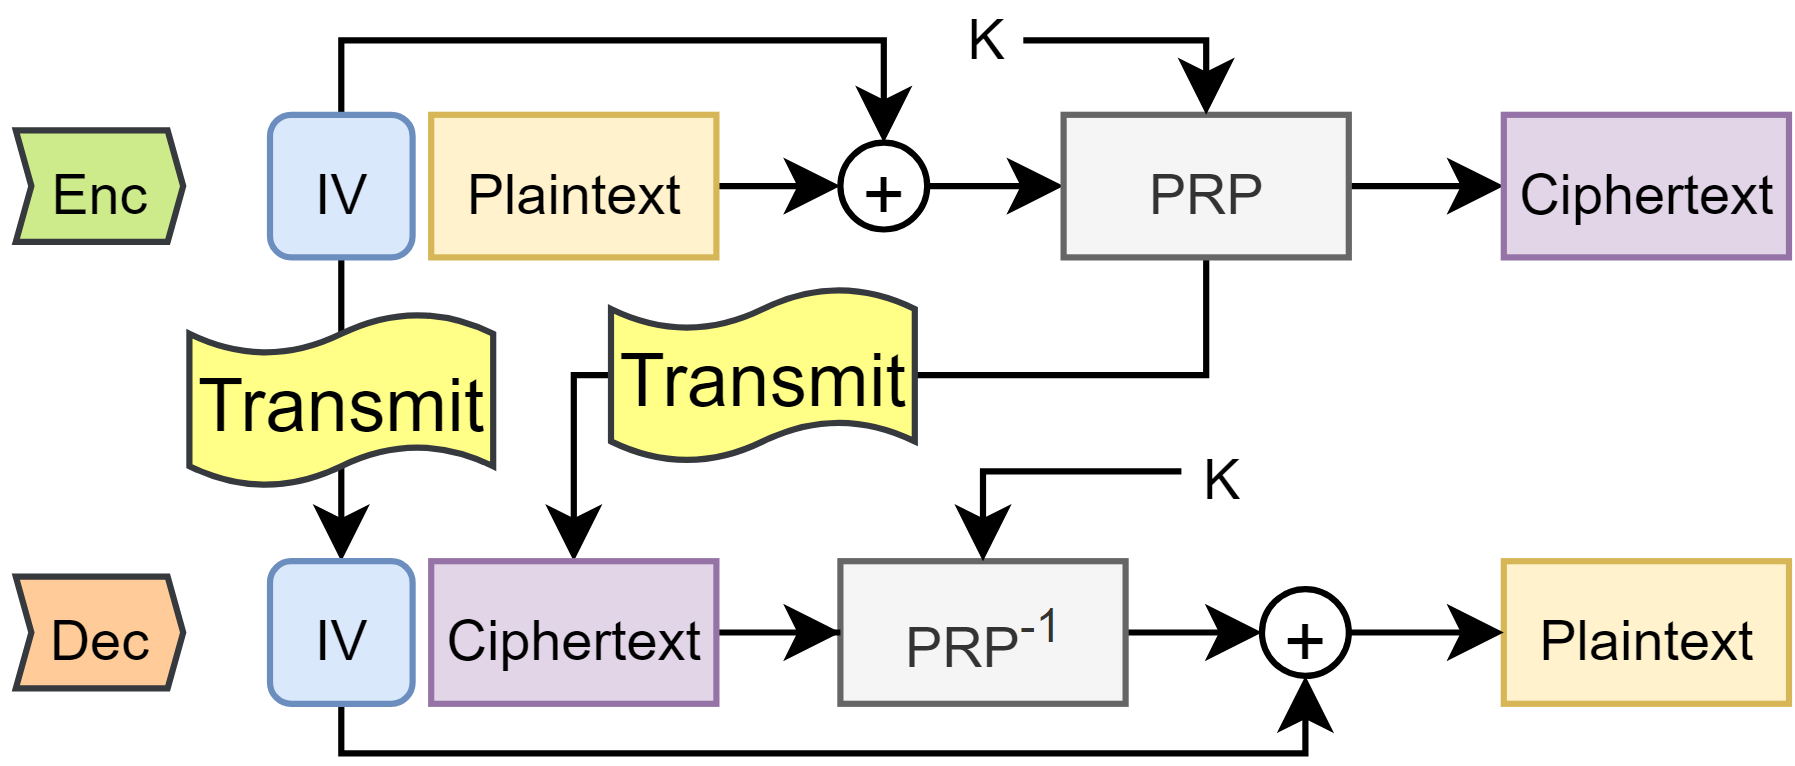
\includegraphics[width=0.8\textwidth]{image/blockiv.png}
    \caption{Block Cipher with IV}
    \label{fig:blockiv}
\end{figure}\\
Le proprietà che adesso dobbiamo richiedere per gli IV sono due:
\begin{theorem}[Semantic Security for ECB]
Se le seguenti proprietà sono soddisfatte abbiamo sicurezza semantica \textit{ECB}.
\begin{property}[IV properties in Block Ciphers]
\begin{itemize}
    \item Gli IV \textbf{NON} devono \textbf{MAI RIPETERSI}.
    \item Gli IV \textbf{DEVONO} essere \text{NON PREDICIBILI}.
\end{itemize}
\end{property}
A patto che:
\begin{itemize}
    \item Il messaggio è più piccolo di un blocco e non si ripete mai.
    \item Gli IV per messaggi ripetuti hanno valori casuali e sono della stessa dimensione di un blocco.
    \item Per messaggi più lunghi di un blocco bisogna combinare i blocchi per non costruire diversi ciphertext.
\end{itemize}
\begin{remark}
L'inconveniente è che dobbiamo trasmettere un messaggio di dimensione doppia: n bit di ciphertext più n di IV. 
\end{remark}
\end{theorem}
\section{Modes of Operations}
I block ciphers vengono suddivisi in categorie in base alla loro \textit{"Modalità di Operazione"}. Le più usate sono \textbf{CBC} e \textbf{CTR} mentre quelle consigliate da usare sono \textbf{CFB} e \textbf{OFB} per alcune particolari proprietà. Ci sono anche due modalità avanzate che forniscono \textit{authenticated encryption}: \textbf{GCM} e \textbf{OCB}.
\begin{note}
Ricordiamo che il problema fondamentale è che gli IV non devono mai ripetersi, quindi è necessario ridurne la generazione, oltre che l'overhead sulla trasmissione.
\end{note}
\pagebreak
\subsection{Cipher Block Chaining: CBC}
Questa modalità si basa su un sistema di block-chain descritto nel modo seguente:
\begin{definition}[Encryption with Cipher Block Chaining Mode]\label{def:cbcenc}
\begin{algorithmic}[1]
\State Divide the plaintext in $n$ chunks.
\State $c[0] = PRP(K,IV\oplus m[0])$\Comment{The IV must be truly rnd}
\For{$i=1$ to $n-1$}
    \State $c[i] = PRP(K, c[i-1]\oplus c[i])$\Comment{$c[i-1]$ is used as IV for $c[i]$}
\EndFor
\State Send \textbf{IV} along with the \textbf{ciphertexts}.
\end{algorithmic}
\end{definition}
Se l\textbf{'IV} è \textbf{truly random} il meccanismo \textbf{è semantic secure} in quanto il primo ciphertext generato sarà una quantità che può essere vista come casuale e tale randomicità verrà trasportata anche ai ciphertext successivi. Pertanto, \textbf{con un solo IV inviato possiamo garantire sicurezza semantica per tutto il messaggio}.\\
Tuttavia le \textbf{cifrature} \textbf{non} sono \textbf{parallelizabili} in quanto le cifrature \textit{i-esime} dipendono da quella successiva e l'ordine delle cifrature è quindi fondamentale. 
\begin{definition}[Decryption with Cipher Block Chaining Mode]\label{def:cbcdec}
\begin{algorithmic}[1]
\State $m[0]=IV\oplus PRP(K,c[0])$
\For{$i=1$ to $n-1$}
\State $m[i] = c[i-1]\oplus PRP(K, c[i])$
\EndFor
\end{algorithmic}
\end{definition}
Osserviamo che il discorso sulla parallelizzazione non sussiste per la decrittazione, in quanto con il solo IV e il messaggio è possibile decifrare tutto il ciphertext in parallelo.
\begin{figure}[h]
    \centering
    \begin{subfigure}[b]{0.48\textwidth}
    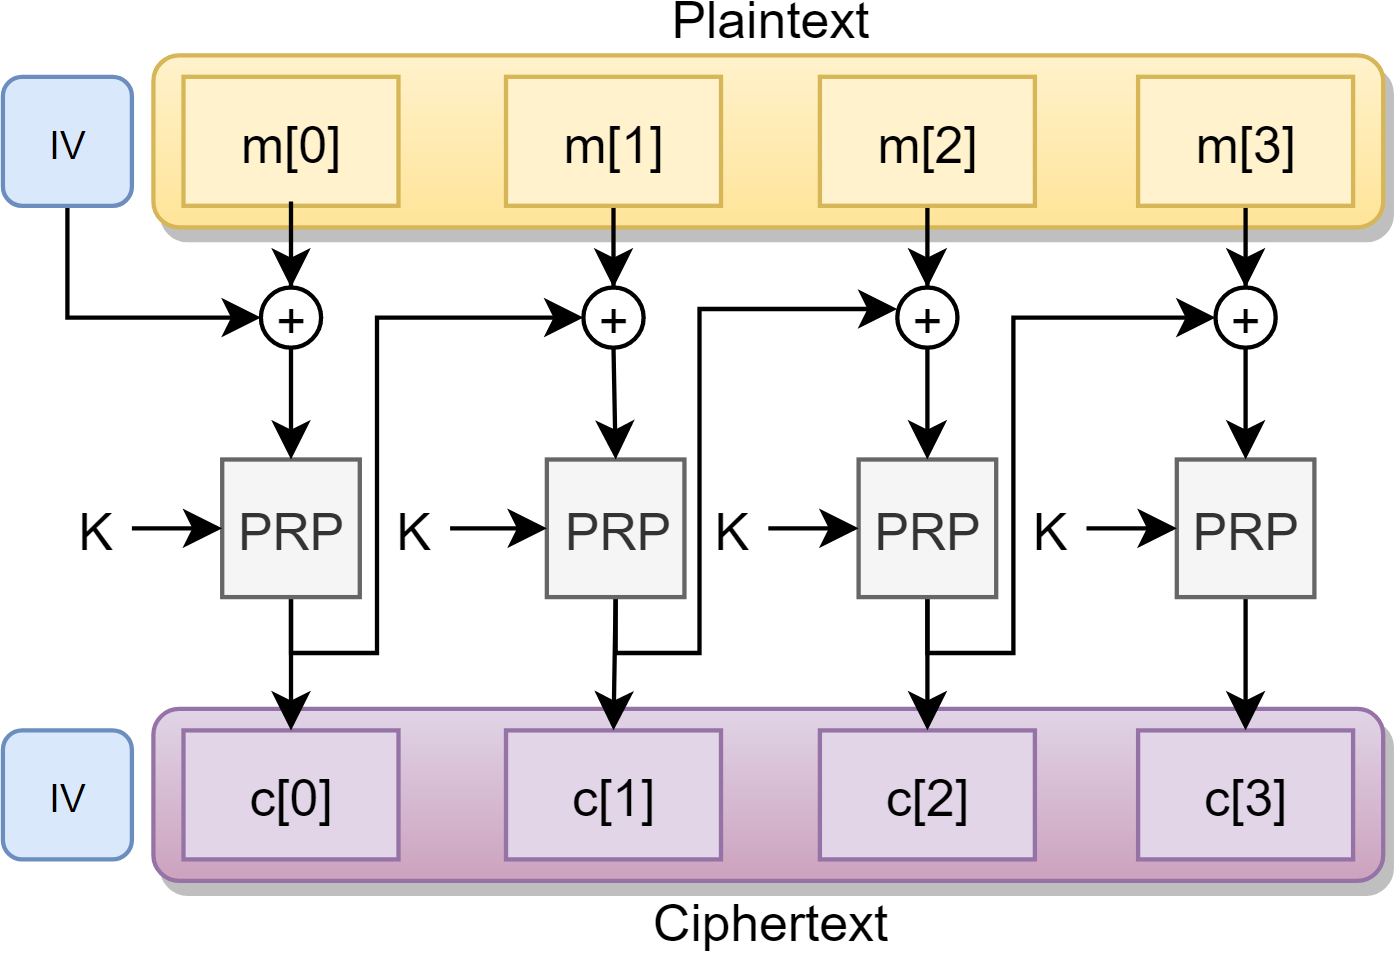
\includegraphics[width=\textwidth]{image/cbcenc.png}
    \caption{CBC Encryption}
    \label{fig:cbcenc}
    \end{subfigure}\quad
    \begin{subfigure}[b]{0.48\textwidth}
    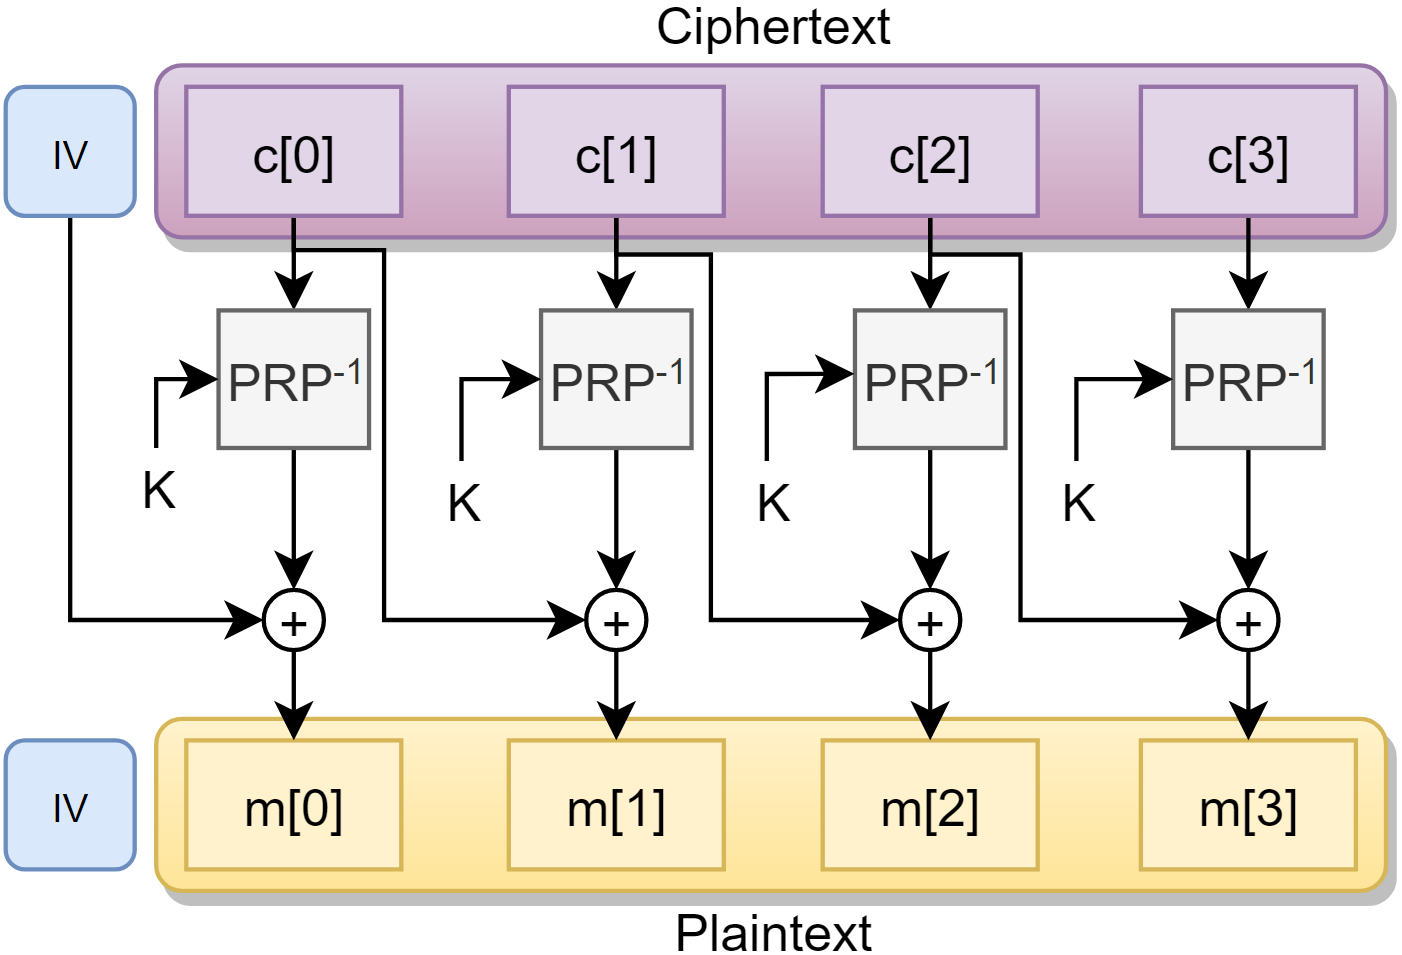
\includegraphics[width=\textwidth]{image/cbcdec.png}
    \caption{CBC Decryption}
    \label{fig:cbcdec}
    \end{subfigure}
    \caption{CBC Mode}
\end{figure}
\begin{note}
CBC è il sistema più comune e usato per cifrare dei messaggi, ma è sicuro sempre se e solo se la nonce è \textbf{truly random e non predicibile}.
\end{note}
\begin{remark}
IV predicibili possono portare a CPA, come successo in \textbf{BEAST} nel 2011.
\end{remark}
\begin{note}
L'implementazione di CBC richiede due circuiti differenti per cifrare e decifrare i messaggi. Poiché questi meccanismi sono spesso inseriti a livello hardware, usare due circuiti significa usare il doppio dello spazio per la realizzazione del sistema di cifratura.
\end{note}
\begin{note}
Poiché lo xor impone che le dimensioni dei chunk siano di un numero fissato, è necessario fare un padding per messaggi che non sono multipli del numero di byte scelto. Il padding viene calcolato secondo degli standard, un esempio è \textbf{PKCS\#7}.
\end{note}
\subsection{Cipher Feedback Mode e Output Feedback Mode}
Le modalità CFB e OFB offrono un punto di vista differente rispetto a CBC. In particolare, tendono ad imitare gli stream ciphers, producendo un keystream utile alla cifratura del plaintext, permettendo di usare un solo circuito, sia per \textit{PRP} che per \textit{PRP\textsuperscript{-1}}.
\begin{definition}[Cipher Feedback Mode - CFB [Encryption]]\label{alg:cfb}
\begin{algorithmic}[1]
\State Assume we have $n$ plaintexts $m[i]\,i=1,\dots,n$.
\State $K_s=\text{ENC}(key, IV)$\Comment{The IV must be truly rnd}
\State $c[0]=m[0]\oplus{K_s}$\Comment{encrypt as stream ciphers with keaystream}
\For{$i=1$ to $n-1$}
    \State $K_s=\text{ENC}(key, c[0])$
    \State $c[i] = c[i-1]\oplus K_s$\Comment{$c[i-1]$ is used as IV for $c[i]$}
\EndFor
\State Send \textbf{IV} along with the \textbf{ciphertexts}.
\end{algorithmic}
\end{definition}
\begin{definition}[Output Feedback Mode - OFB [Encryption]]\label{alg:ofb}
\begin{algorithmic}[1]
\State Assume we have $n$ plaintexts $m[i]\,i=1,\dots,n$.
\State $K_s[0]=\text{ENC}(key, IV)$\Comment{The IV must be truly rnd}
\For{$i=0$ to $n$}
    \State $c[i]=m[0]\oplus{K_s}$\Comment{encrypt as stream ciphers with keaystream}
    \State $K_s[i]=\text{ENC}(key, K_s[i-1])$ \Comment{$K_s[i-1]$ is used as IV for $K_s[i]$}
\EndFor
\State Send \textbf{IV} along with the \textbf{ciphertexts}.
\end{algorithmic}
\end{definition}
Sia CFB che OFB cifrano il messaggio mascherandolo con un keystream generato tramite un \textbf{\textit{block cipher encryptiion}} senza la necessità di fare padding. L'\textbf{encryption non} è \textbf{parallelizzabile} in nessuno dei due casi ma \textbf{OFB permette} di fare \textbf{preprocessing} in quanto lo stato del messaggio cifrato non dipende da quello precedente e i keystream possono essere calcolati in blocco.\\
Per fare decryption è possibile usare lo stesso circuito di encryption, dove \textbf{CFB} è in vantaggio perché \textbf{permette} di \textbf{parallelizzare} il processo.
\begin{definition}[CFB Decryption]
\begin{algorithmic}[1]
\State Assume we have \textit{n} ciphertexts.
\State Take the \textit{IV} from arriving message.
\State $K_s[0] = ENC(IV, k)$
\ForAll{ciphertexts}
\State $m[i] = K_s[i-1]\oplus{c[i]}$\Comment{Get the Plaintext}
\State $K_s[i] = ENC(c[i-1], k)$\Comment{Generate Keystream from $c[i-1]$}
\EndFor
\end{algorithmic}
\end{definition}
\begin{definition}[OFB Decrption]
\begin{algorithmic}[1]
\State Assume we have \textit{n} ciphertexts.
\State Take \textit{IV} from arriving message.
\State $K_s[0] = ENC(IV, k)$
\ForAll{ciphertexts}
\State $m[i] = K_s[i-1]\oplus{c[i]}$\Comment{Get the Plaintext}
\State $K_s = ENC(K_s[i-1], K)$\Comment{Generate Keystream from $K_s[i-1]$}
\EndFor
\end{algorithmic}
\end{definition}

\begin{figure}[h]
    \centering
    \begin{subfigure}[b]{0.48\textwidth}
    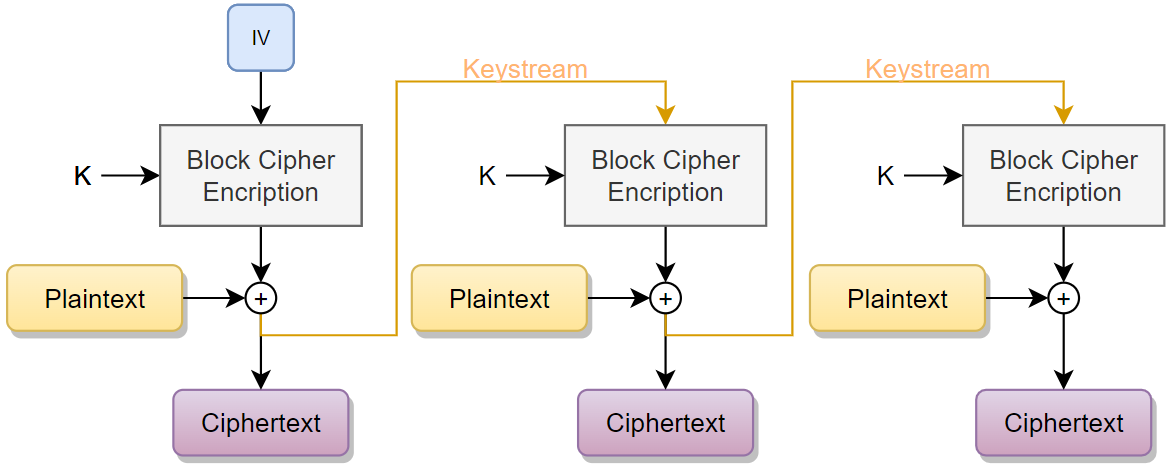
\includegraphics[width=\textwidth]{image/cfbenc.png}
    \caption{Encryption}
    \label{fig:cfbenc}
    \end{subfigure}\quad
    \begin{subfigure}[b]{0.48\textwidth}
    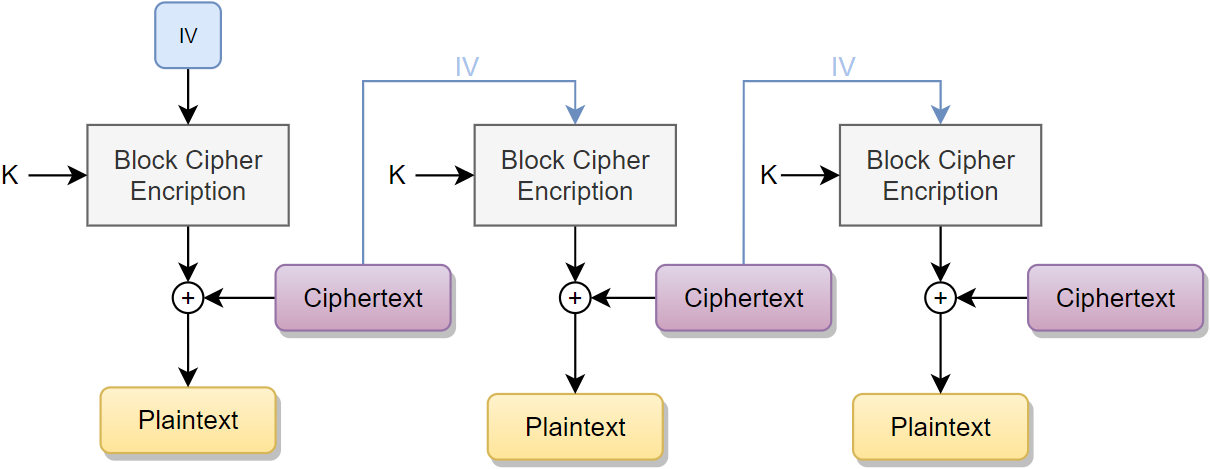
\includegraphics[width=\textwidth]{image/cfbdec.png}
    \caption{Decryption}
    \label{fig:cfbdec}
    \end{subfigure}
    \caption{Cipher Feedback Mode}
\end{figure}
\begin{figure}[h]
    \centering
    \begin{subfigure}[b]{0.48\textwidth}
    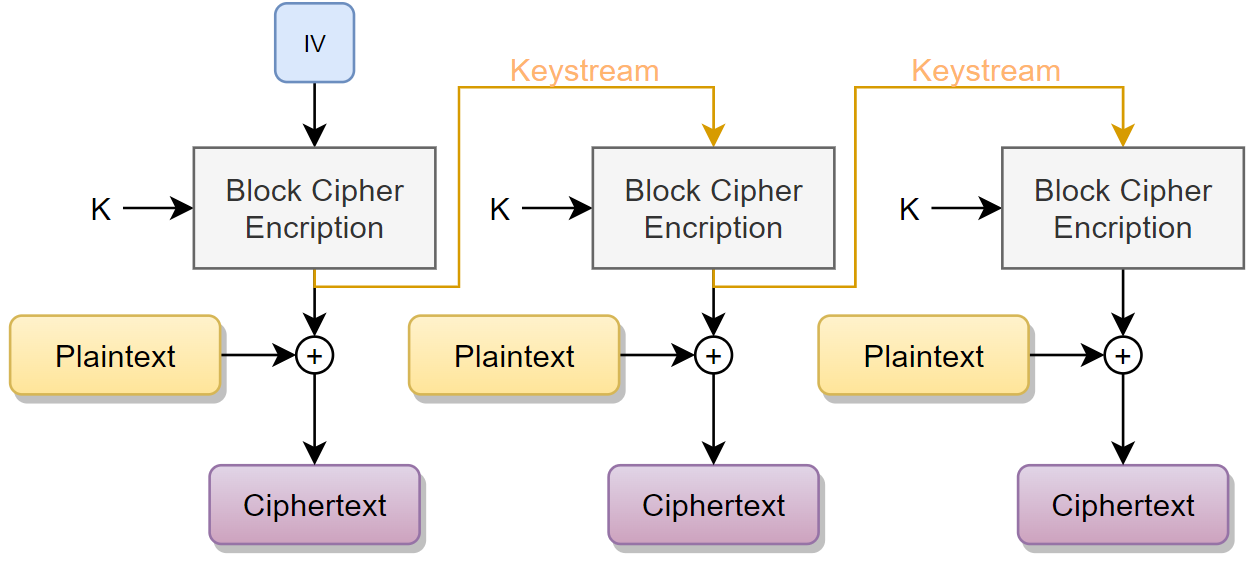
\includegraphics[width=\textwidth]{image/ofbenc.png}
    \caption{Encryption}
    \label{fig:ofbenc}
    \end{subfigure}\quad
    \begin{subfigure}[b]{0.48\textwidth}
    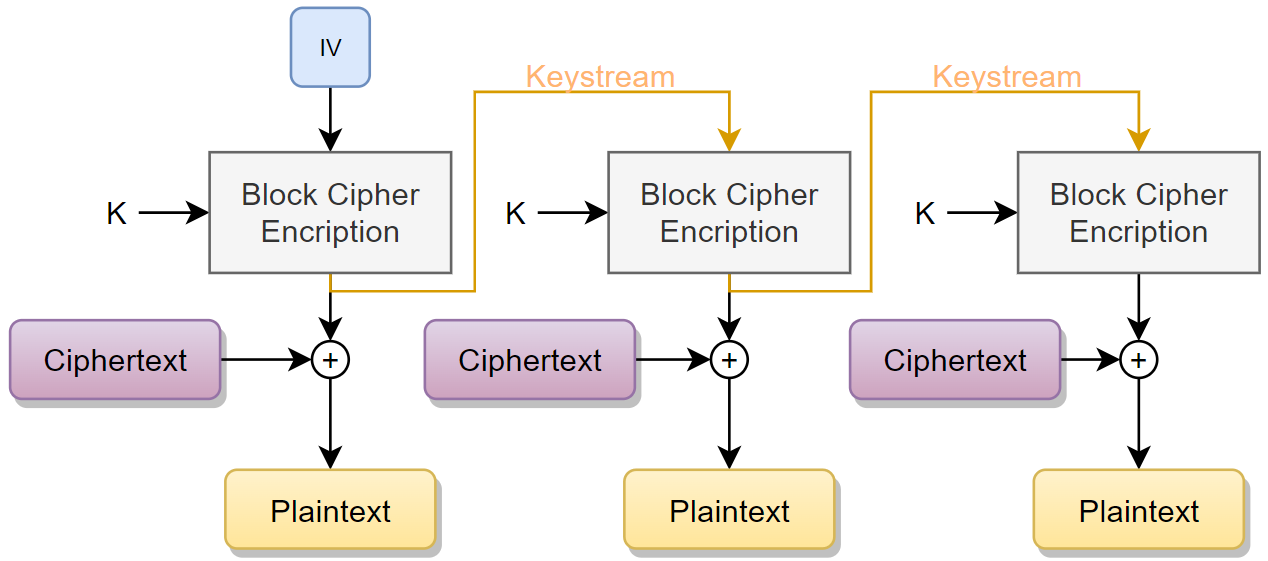
\includegraphics[width=\textwidth]{image/ofbdec.png}
    \caption{Decryption}
    \label{fig:ofbdec}
    \end{subfigure}
    \caption{Output Feedback Mode}
\end{figure}
\section{Short Cycle Problem}
I cifratori a blocchi dipendono fortemente dal blocco di encryption che calcola la pseudorandom permutation. Questo implica che la funzione che scegliamo per calcolare la permutazione deve essere fatta bene e robusta anche a specifiche condizioni iniziali. In particolare, non possiamo usare funzioni che soffrono del:
\begin{definition}[Short Cycle Problem]\label{def:shortcycle}
Condizione per la quale un algoritmo di cifratura, a partire da alcune specifiche condizioni iniziali, tendono a ripetere i valori di ciphertext dopo poco tempo.
\end{definition}
\begin{example} Consideriamo l'insieme $S$ e la permutazione seguente $\prod$.
\begin{figure}[h]
    \centering
    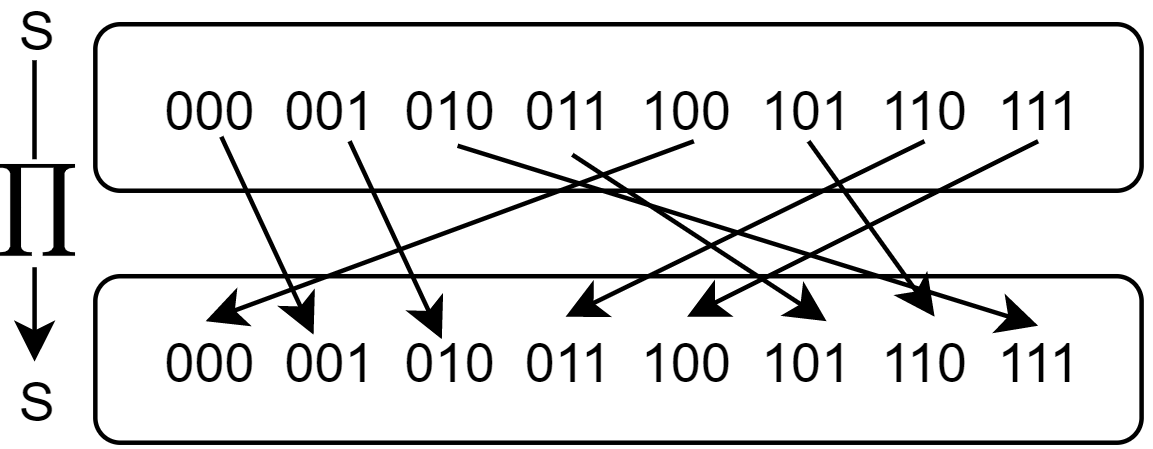
\includegraphics[width=0.5\textwidth]{image/shortcycle.png}
    \caption{PRP function for 3-bit blocks}
    \label{fig:shortcycle}
\end{figure}
\begin{enumerate}
    \item \textbf{OFB} con $IV=010$: $C=010\,111\,100\,001$ \textcolor{red}{$010\,111\,\dots$}\\
    I valori di $C$ cominciano a ripetersi dopo 5 iterazioni.
    \item \textbf{OFB} con $IV=011$: $C=011\,101\,110$ \textcolor{red}{$011\,101\,110\,\dots$}\\
    I valori di $C$ cominciano a ripetersi dono 3 iterazioni.
\end{enumerate}
\end{example}
\begin{example}Vediamo che anche \textbf{CBC} presenta gli stessi problemi se cifra un testo con delle ripetizioni: 
\begin{itemize}
    \item $P=011\,011\,011$ con $IV:010$: \textcolor{red}{$C=(010)\,010\,010\,010$}
\end{itemize}
\end{example}
\section{Counter Mode}
Poiché le modalità precedenti sono soggette allo \textit{short cycle problem} una modalità resistente è necessaria. In particolare, poiché il problema è intrinseco all'\textit{IV} scelto per avviare la cifratura, se questo fosse sviluppato dinamicamente e sempre diverso, non potremmo avere cicli all'interno di una sequenza di cifratura.\\
Assumendo l'\textit{IV} come un \textbf{contatore} incrementato ad ogni nuovo blocco, è possibile dimostrare che se la PRP è sicura, allora il risultato pseudorandomico generato è sicuro.
\begin{note}
La modalità \textit{CTR} gode della maggior parte dei vantaggi:
\end{note}
\begin{enumerate}
    \item [\textcolor{green}{\checkmark}]Trasforma i block-cipher in stream-cipher.
    \item [\textcolor{green}{\checkmark}]Combina i vantaggi di \textit{CFB}(\cref{alg:cfb}) e \textit{OFB}(\cref{alg:ofb}).
    \item [\textcolor{green}{\checkmark}]Permette un'implementazione efficiente (sia \textit{HW} che \textit{SW}) utilizzando parallelizzazione sia in encryption che decryption.
    \item [\textcolor{green}{\checkmark}]Richiede l'implementazione di un singolo blocco di cifratura per entrambe le operazioni.
    \item [\textcolor{green}{\checkmark}]Permette di attuare meccanismi di \textbf{Random Access} (ad esempio a sistemi di memoria cifrata) poiché la decrittazione del blocco \textit{i-esimo} non dipende dai precedenti.
    \item [\textcolor{green}{\checkmark}]E' sicuro se usiamo accortezze sui contatori.
    \item [\textcolor{green}{\checkmark}]Viene garantita robustezza allo Short Cycle Problem (\cref{def:shortcycle}).
\end{enumerate}
\begin{definition}[Counter Mode Encryption/Decription]\label{def:ctrmode}
\begin{algorithmic}[1]
\State Assume we have \textit{n} plaintext/ciphertext
\State Initialize a counter $ctr$ as standard specifies\footnotemark.
\ForAll{plaintexts}
\State $K_s[i] = ENC(ctr,K)$
\State $c[i] = K_s[i]\oplus{m[i]}$
\State $ctr = ctr + 1$
\EndFor
\end{algorithmic}
\footnotetext{\textsuperscript{\thefootnote}Ad esempio AES-CTR specifica che per l'\textbf{Initial Counter Block} il contatore è formato \textbf{da 128bit} dove i \textbf{primi 96} sono costituiti dall'\textbf{IV} e i \textbf{restanti 32} dal \textbf{contatore}, \textbf{partendo da 1}.}
\end{definition}
\begin{figure}[h]
    \centering
    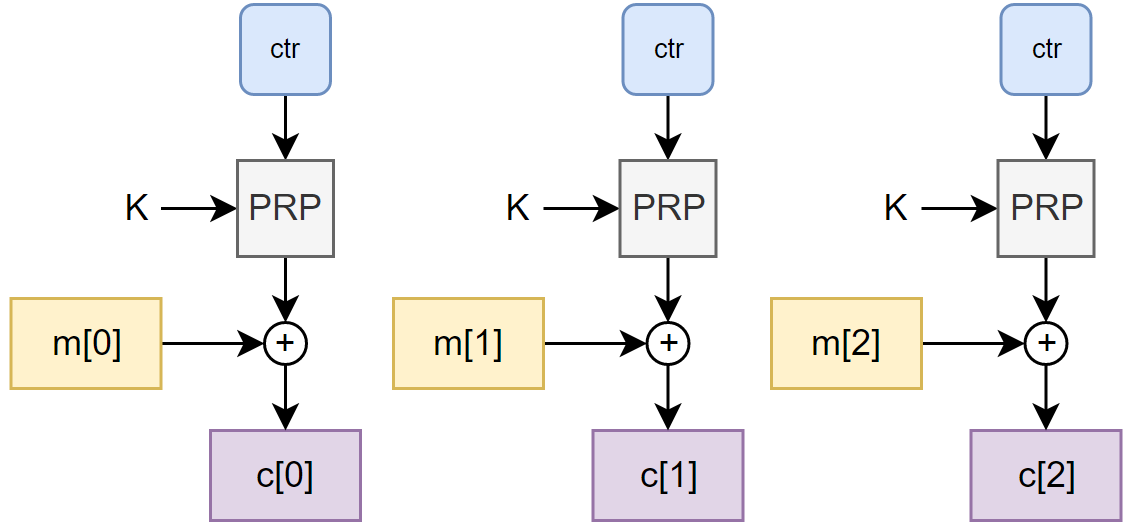
\includegraphics[width=0.8\textwidth]{image/blkctr.png}
    \caption{Counter Mode Block Cipher}
    \label{fig:ctrmode}
\end{figure}


\chapter{Authenticated Encryption with Associated Data}\label{chap:aead}
Sappiamo che un cifratore ben strutturato può garantire \textit{confidentiality}, ovvero abbiamo semantic security contro attacchi \textit{CPA}. Tuttavia, per garantire \textit{integrity} abbiamo fatto fino ad ora un discorso separato, basato su un codice generato tramite una funzione hash.\\ 
\begin{remark}
Se un attaccante dovesse essere \textit{"attivo"}, ovvero in grado di creare un testo cifrato il cui MAC sia valido, non avremmo modo di garantire \textit{integrity}.
\end{remark}
\begin{definition}[Chosen Ciphertext Attack]\label{def:cca}
Scenario di attacco nel quale un hacker può fare, oltre all'eavesdropping, anche una cifratura di un plaintext di sua creazione che è in grado di modificare un messaggio.\\
\textbf{Rompendo}, di fatto, \textbf{sia confidentiality che integrity}.
\end{definition}
Vediamo due esempi di come \textbf{rompere confidentiality} porti ad una \textbf{rottura di integrity}.
\begin{example}Consideriamo l'invio di un pacchetto \textit{TCP/IP} da \textit{\textbf{A}} verso \textit{\textbf{B}} passando per un web-server che gestisce lo stack TCP/IP. Facciamo le seguenti supposizioni: 
\begin{enumerate}
    \item Il pacchetto attraversa un server sul quale \textit{\textbf{E}} può intercettare i processi su una porta specifica. Per semplicità il \textbf{pacchetto} sia \textbf{diretto} sulla \textbf{porta 80 di B}, mentre \textbf{E} può \textbf{leggere} dalla \textbf{porta 25}. 
    \item Il canale di trasferimento è \textbf{protetto} con \textbf{sola encryption} (garantiamo solo \textit{confidentiality}).
    \item L'attaccante è in grado di generare un cipher-text il cui contenuto cambia la porta da 80 a 25. 
\end{enumerate}
Poiché non ci stiamo preoccupando di integrity (e quindi non usiamo un MAC), \textit{\textbf{E}} può leggere i dati in chiaro dal server dalla porta 25. In particolare, se viene usato \textbf{AES-CBC} è semplice in quanto basta fare uno xor. Vediamo lo schema:
\begin{figure}[h]
    \centering
    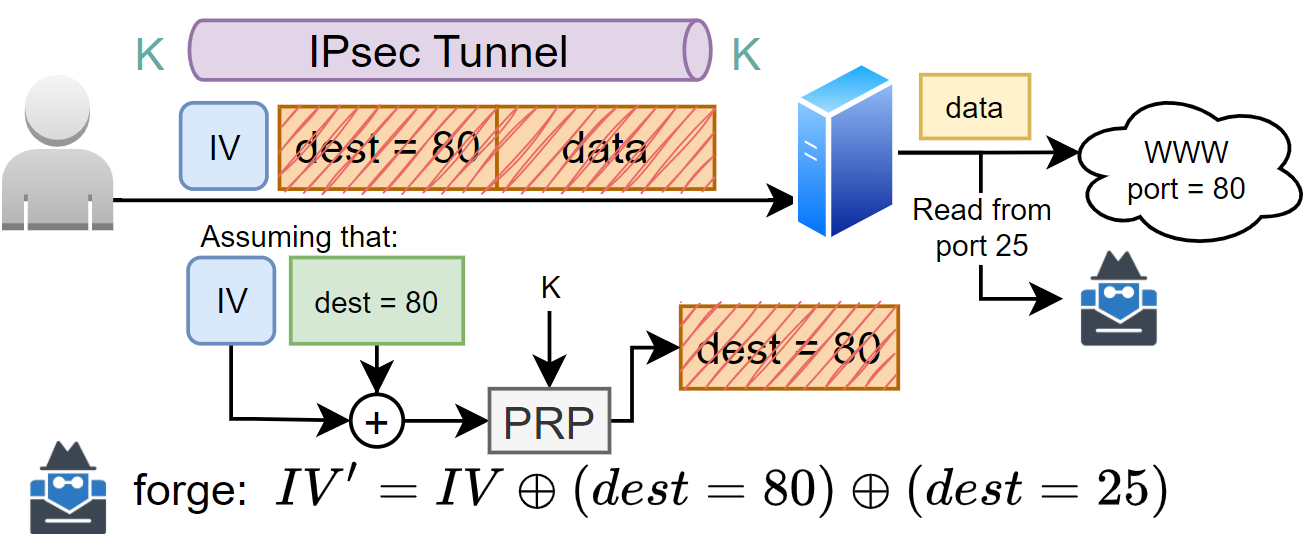
\includegraphics{image/portredirect.png}
    \caption{Broken Confidentiality}
    \label{fig:portredirect}
\end{figure}\\
Inserendo l'\textit{IV'}, nel processo di cifratura possiamo cambiare la porta. Infatti:
\begin{figure}[ht]
    \centering
    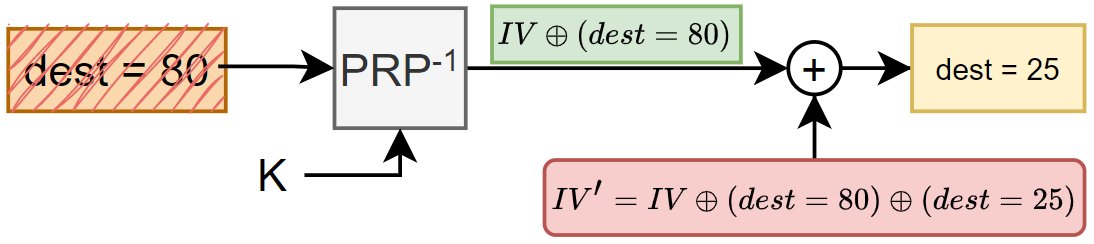
\includegraphics{image/portredirectdec.png}
    \caption{Decription}
    \label{fig:decriptionport}
\end{figure}
\end{example}
\begin{example}[ ACK-Oracle:]Supponiamo che A stia usando una \textit{remote terminal app}, dove ogni keystroke viene cifrato in CTR e inviato verso un server. I \textit{"poteri"} di E sono i seguenti:
\begin{enumerate}
    \item \textbf{E non ha accesso al backend}.
    \item La cifratura viene fatta in CTR mode.
    \item L'header è tipicamente noto poiché la struttura è definita da standard e i valori possono essere predetti.
    \item E può copiare il messaggio cifrato di A.
    \item [\textcolor{red}{FACT}:]Lo stack TCP/IP processa solo pacchetti validi, rispondendo con un \textit{ACK} solo ai pacchetti con checksum valido. Il checksum è calcolato in funzione dell'header del pacchetto e del carattere inviato D.
\end{enumerate}
\begin{note}
Il protocollo restituisce pertanto \textbf{DUE} risultati, indicandoci quali sono i pacchetti corretti e non rispondendo nulla se il pacchetto non lo è.
\end{note}
Supponiamo di fare molte copie del messaggio e di provare $\forall{t,s}$ ad inviare verso il server una copia modificata nel campo checksum e carattere calcolando $checksum\oplus{t}$ e $D\oplus{s}$. Per ogni volta in cui il server dello stack TCP/IP risponderà con un ACK, otteniamo un'equazione valida del tipo:
\[checksum(pkt-hdr,D\oplus{s})=t\oplus{cheksum(pkt-hdr, D)}\]
Poiché l'header del pacchetto è noto (punto 3), mentre la coppia {checksum, D} non lo è, il sistema è risolubile. Una volta trovata una soluzione, è facile risalire al checksum e a D in base alla struttura con cui è calcolato il checksum. 
\end{example}
\begin{remark}
Dagli esempi capiamo che non bisogna \textbf{MAI} usare un meccanismo di encryption da solo\footnotetext{A meno di alcuni casi speciali chiamati \textit{\textbf{Homomorphic Encryption.}}} ma bisogna sempre aggiungere un servizio di integrity, in particolare, \textbf{SI DEVE} usare \textbf{SOLO} authenticated encryption.
\end{remark}
\section{Meccanismi di AE}
Gli algoritmi di AE producono un ciphertext di lunghezza maggiore del plaintext di partenza in quanto oltre al testo cifrato devono includere \textbf{\textit{anche}} il tag di auth. 
\begin{note}
E' impossibile, per un meccanismo di AE, produrre un ciphertext di lunghezza pari al plaintext.
\end{note}
Per costruzione gli algoritmi di AE verificano se il messaggio è valido e, successivamente, rispondono in due modi:
\begin{itemize}
    \item [\textcolor{green}{\checkmark}] Il messaggio originale.
    \item [\textcolor{red}{\ding{55}}] Un messaggio di \textbf{\textit{REJECT}}.
\end{itemize}
\begin{proposition}
Gli algoritmi di Authenticated Encryption decifrano il messaggio \textbf{se solo se} il tag è valido.
\end{proposition}
Possiamo dare una definizione di sicurezza per un algoritmo di authenticated encryption:
\begin{definition}[Sicurezza per AE]\label{def:ae}
Un algoritmo di Authenticated Encryption è sicuro se:
\begin{itemize}
    \item E' semantically secure sotto CPA.
    \item Garantisce integrity del ciphertext: la probabilità che un messaggio cifrato generato dall'avversario venga decifrato\footnotemark deve essere trascurabile. 
    \footnotetext{\textsuperscript{\thefootnote}Consideriamo un successo anche se il messaggio cifrato viene decifrato in un messaggio completamente casuale.}
\end{itemize}
\end{definition}
\begin{note}
Il meccanismo \textbf{Encrypt-than-MAC} soddisfa \cref{def:ae} ma non è di tipo \textit{AEAD}
\end{note}
\begin{example}[ Semantic security against Chosen Ciphertext Attack Model]\hfill\\
Consideriamo un esempio simile a quello di \cref{fig:ciphertextoracle} dove questa volta il meccanismo di risposta è diverso in quanto il risultato della decrittazione del chosen ciphertext può essere un success o un reject. Supponiamo ovviamente che l'avversario non conosca la chiave di cifratura ma scegliendo i plaintext di una challenge è in grado di ottenere dei ciphertext in risposta, come se il challenger fosse un oracolo.\\
La mappa ottenuta permette all'avversario di generare un ciphertext diverso dai precedenti (ad esempio facendo combinazioni lineari/non lineari dei $c_i$ precedenti), che una volta inviato come nuovo messaggio se viene decifrato in una forma qualsiasi di plaintext (sensato o meno) costituisce un indizio per l'avversario in quanto ha generato un messaggio valido.
\end{example}
\begin{figure}[h]
    \centering
    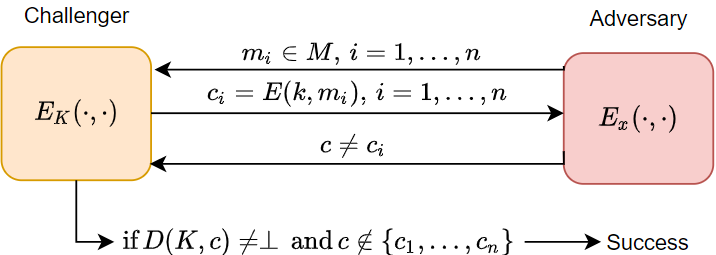
\includegraphics[width=0.8\textwidth]{image/cca.png}
    \caption{CCA Oracle game}
    \label{fig:ciphertextoracle}
\end{figure}\pagebreak
\subsection{Associated Data}
Quando trasmettiamo dei dati c'è spesso la necessità di trasmettere una parte dei dati in chiaro, ad esempio in un pacchetto TCP/IP il cui header può restare in chiaro. Quello che vorremmo però è che l'autenticazione venga fatta \textbf{su tutto} il pacchetto.\\
Possiamo avere due casi limite, tipicamente:
\begin{itemize}
    \item No Associated Data: è sufficiente CCA-Secure Encryption, quindi tutto è cifrato.
    \item No Encrypted Data: è sufficiente un MAC costruito in modo sicuro (\cref{def:hmac}). 
\end{itemize}
Gli algoritmi di AEAD possono lavorare in modo diverso:
\begin{itemize}
    \item Two-Layer: prima cifro e poi applico MAC \textit{(es: AES-GCM)}.  Poiché servono due iterazioni, è un meccanismo più lento e non parallelizzabile poiché per produrre il MAC serve il ciphertext.
    \item One-Layer: faccio cifratura e MAC contemporaneamente \textit{(es: OCB)}. Più veloce \textit{(online cipher)}.
\end{itemize}
\begin{note}
Le performance sono fondamentali al giorno d'oggi visto che è file sono grandi giga e giga. 
\end{note}
Ad ogni modo, possiamo osservare due problemi fondamentali:
\begin{problem}[ Dove posizionare la parte di Associated Data?]Tipicamente non c'è una risposta, poiché dipende dal protocollo. Ad esempio se parliamo di header dovrà andare in testa, in altri casi alla fine o anche un mix tra la parte di cifratura e in chiaro. 
\end{problem}
\begin{problem}[ Misuse Resistance]
Quanto è robusto un meccanismo di AEAD quando un IV si ripete?
\end{problem}
\vspace{-5mm}
\section{AES-GCM: Galois Counter Mode}
\vspace{-5mm}
Algoritmo usato nella maggior parte dei protocolli di sicurezza come IPsec e TLS, che usa una struttura \textbf{Enc-than-MAC}. 
\begin{itemize}
    \item \textbf{Encryption:} AES-CTR (\cref{def:ctrmode}).
    \item \textbf{MAC:} GHASH function. Non una crypto-hash ma una struttura algebrica \footnotetext{\href{https://it.wikipedia.org/wiki/Campo_finito}{Galois Field}} per fare prodotti tra polinomi in modo molto veloce. \textbf{Non garantisce sicurezza crittografica}.
\end{itemize}\begin{figure}[h]
    \centering
    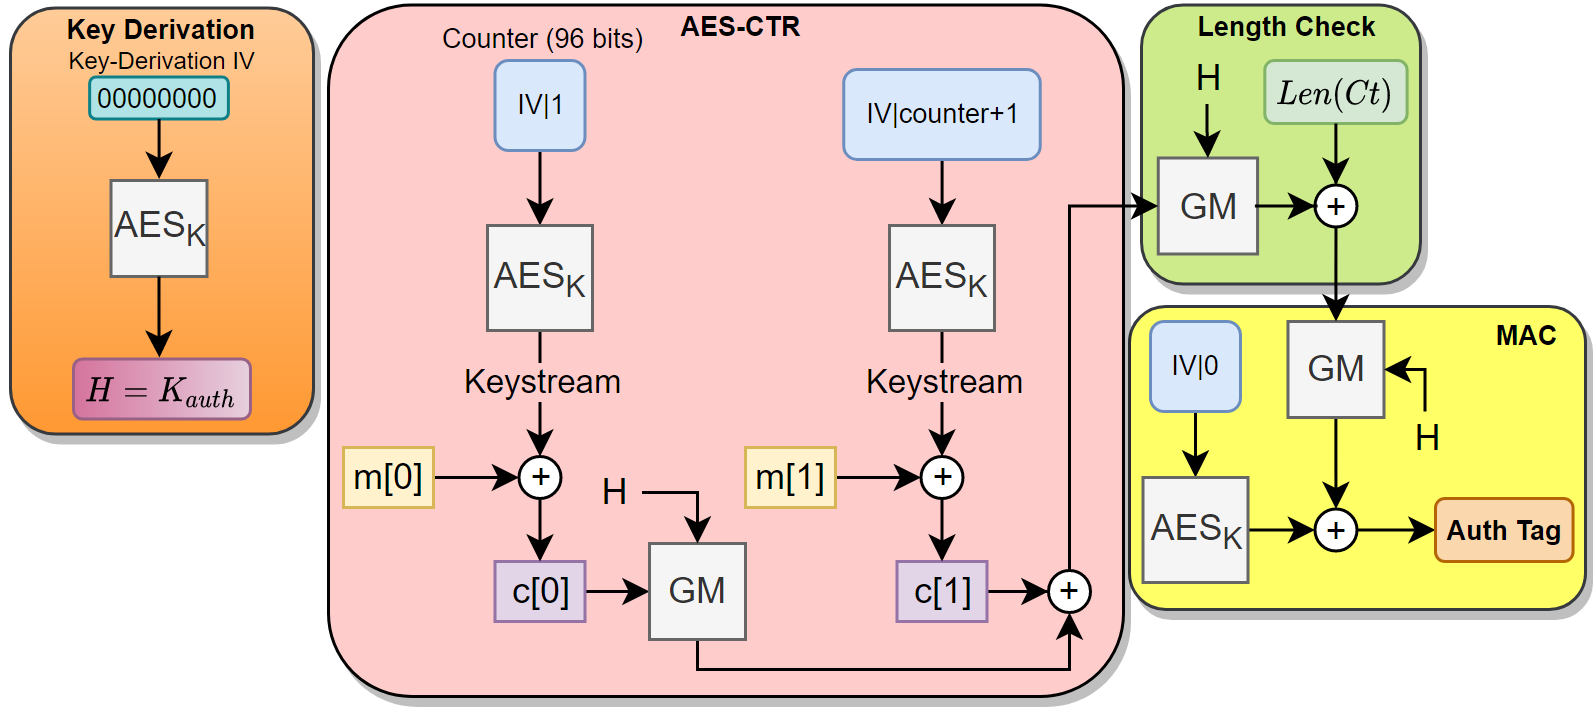
\includegraphics{image/aesgcm.png}
    \caption{AES-GCM scheme}
    \label{fig:aesgcm}
\end{figure}

\begin{definition}[AES-GCM - Galois Counter Mode]\label{def:aesgcm}
Data la chiave $K$, AES-GCM opera nel seguente modo:
\begin{itemize}
    \item \textbf{Key-Derivation:} Poiché la \textbf{chiave} di \textbf{cifratura} \textbf{DEVE} essere \textbf{diversa} \textbf{da} quella di \textbf{autenticazione}, produciamo una chiave $H$, usata per produrre il MAC.
    \item \textbf{AES-CTR:} La parte di cifratura del messaggio viene svolta come in CTR\footnotemark (\cref{def:ctrmode}) \textbf{partendo da 1}, ma ogni ciphertext ottenuto produce un MAC ottenuto tramite il blocco $GM(H)$ per mezzo di prodotti tra polinomi. Il MAC ottenuto va in xor con il ciphertext sucecssivo per produrre un nuovo MAC.
    \item \textbf{Lenght-Check:} Alla fine della cifratura, l'ultimo MAC prodotto viene messo in xor con la lunghezza del ciphertext complessivo per produrre un nuovo MAC. 
    \begin{note}
    L'aggiunta del controllo sulla lunghezza protegge la costruzione del MAC da un expansion attack.
    \end{note}
    \item \textbf{Wegman-Carter MAC:} Il MAC della lunghezza viene messo in xor con un keystream ottenuto in CTR-mode ma con contatore $0$ per produrre un MAC \textbf{sicuro}. 
    \begin{note}
    L'IV usato a questo step sarà \textbf{SEMPRE} diverso in quanto il contatore iniziale era 1. 
    \end{note}
\end{itemize}
\footnotetext{\textsuperscript{\thefootnote}Il blocco $AES_k$ è una Pseudo-Random Function (PRF).}
\end{definition}
\begin{corollary}[Wegman-Carter Construction]\label{cor:wegmancarter}

Il MAC costruito tramite GCM è una costruzione di tipo Wegman-Carter. Questa costruzione ci fornisce un modo di creare un codice di autenticazione anche quando \textbf{non usiamo} delle funzioni crittografiche. Abbiamo però bisogno di due elementi fondamentali:
\begin{itemize}
    \item Funzioni Hash \textbf{Universali}.
    \item Pseudo Random Functions.
\end{itemize}
\end{corollary}
Le funzioni hash universali sono una famiglia di funzioni dette \textbf{"Key-Hash Function"} il cui output \textbf{dipende} dalla specifica chiave con cui la funzione è inizializzata. In particolare:
\begin{definition}[Universal Hash Functions]
Una famiglia di Key-Hash Function è detta universale se è difficile, per un attaccante che \textbf{non conosce la chiave}, trovare una collisione tale che $H_k(M_1)=H_k(M_2)$.\\
Analogamente: $\forall{x,y}\,:\,x\ne{y}\, Prob\{H_x(M)=H_y(M)\}\leq{1/m}$, con $m$ dimensione del digest. 
\end{definition}
Rispetto ad una crypto hash, le differenze principali stano nel fatto che 
\begin{itemize}
    \item \textbf{se la chiave è nota} trovare una collisione  \textbf{può essere facile}.
    \item L'output \textbf{potrebbe non essere} pseudorandomico.
    \item Dalla seconda proprietà: Un cambio di chiave dovrebbe provocare un cambio nel digest in modo causale e quindi ridurre drasticamente la probabilità di collisione.
    \item Dalla seconda proprietà: Non dovrebbero esserci coppie di messaggi che producono lo stesso hash per chiavi diverse. 
\end{itemize}\pagebreak
\begin{note}\textbf{Come tratto la parte di Dati Associati?}\hfill\\
Semplice: Per ogni blocco di AD produco un MAC che va in xor con il blocco successivo per produrre un nuovo MAC. Alla fine della parte di AD, il MAC va in xor con il primo ciphertext e si continua come indicato in \cref{fig:aesgcm}. La differenza \textbf{sostanziale} sta nell'\textbf{allungare} la dimensione del messaggio complessivo, che ora deve comprendere anche la parte di AD.
\end{note}
\subsection{Misuse Resistance per GCM}
La costruzione trovata è utile ma ha un problema \textbf{fondamentale:} \textbf{E' LINEARE}, su due aspetti. 
\begin{enumerate}
    \item Il tag è lineare in xor in quanto: $tag=GHASH_H(CT)\oplus{AES_K(IV,0)}$. Pertanto, dati due tag
    \begin{equation*}
        \begin{aligned}
            tag_1&=GHASH_H(CT_1)\oplus{AES_K(IV,0)}\\
            tag_2&=GHASH_H(CT_2)\oplus{AES_K(IV,0)}\\
            tag_1\oplus{tag_2}&=GHASH_H(CT_1)\oplus{GHASH_H(CT_1)}
        \end{aligned}
    \end{equation*}
    \item Poiché la GHASH function usa una moltiplicazione tra polinomi, un attaccante può sempre recuperare la chiave di auth e forgiare dei messaggi validi (\textit{\textbf{la chiave $K$ comunque rimane segreta}}.
\end{enumerate}
Esistono chiaramente delle costruzioni più robuste quando si verifica il riutilizzo di una nonce, ma non le trattiamo in questo momento.
\chapter{Asymmetric Cryptography}
Per poter \textbf{instaurare} una \textbf{comunicazione sicura} tra due entità che \textbf{non} possiedono un \textbf{segreto comune} è \textbf{necessario} utilizzare algoritmi che non riveli ad entità terze in rete alcun segreto critico.\\
Questi algoritmi sono detti \textbf{a Chiave Asimmetrica}, ovvero algoritmi dove le chiavi di encryption e decryption sono \textbf{legate} ma \textbf{differenti}. Distinguiamo in \textbf{chiave pubblica} e \textbf{privata}.
\begin{figure}[h]
    \centering
    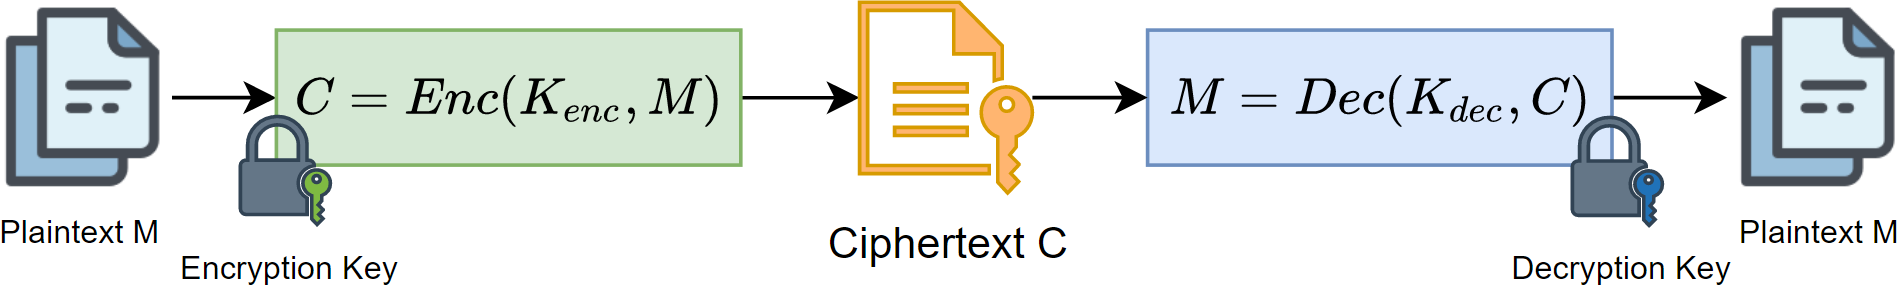
\includegraphics{image/asimmcrypto.png}
    \caption{Asymmetric Encryption Base Scheme}
    \label{fig:asymmcrypto}
\end{figure}
C'è un \textbf{importante MA:} gli algoritmi a chiave asimmetrica sono \textbf{computazionalmente onerosi} e non sarebbero praticabili per l'\textbf{intera} sessione di comunicazione cifrata.\\
C'è bisogno di un approccio \textbf{ibrido}:
\begin{itemize}
    \item Algoritmi Asimmetrici per \textbf{inizializzare} la comunicazione \textbf{sicura}
    \item Algoritmi Simmetrici per il \textbf{trasferimento sicuro} di informazioni.
\end{itemize}
\begin{definition}[Hybrid Approach for Persistent Communication]
\begin{enumerate}
    \item \textbf{Handshake/Session Key Exchange:} Viene utilizzata la \textbf{criptazione asimmetrica} per \textbf{scambiarsi informazioni} sulla \textbf{crittografia simmetrica} da utilizzare successivamente e \textbf{impostare} dei \textbf{segreti comuni (Key Agreement)} tra le due parti.\\
    \begin{remark}
    Dai segreti comuni vengono derivate le chiavi simmetriche, dette \textbf{Chiavi di Sessione}, usate nella\textbf{ criptazione simmetrica} e nel \textbf{controllo di integrità}.
    \end{remark}
    \item \textbf{Data Transfer:} le due parti \textbf{comunicano} in maniera sicura tra loro, tramite \textbf{meccanismi a chiave simmetrica}.
    \item \textbf{Rekeying:} eventualmente vengono \textbf{derivate nuove chiavi simmetriche} dagli \textbf{stessi} segreti comuni impostati precedentemente.
\end{enumerate}
\end{definition}
\section{Public Key Encryption \& Digital Signature}
Gli algoritmi asimmetrici utilizzano la \textbf{chiave} che viene condivisa, ovvero resa \textbf{pubblica}, durante la trasmissione dei dati. Poiché le chiavi pubbliche e private sono legate, vale la seguente proprietà:
\begin{proposition}[Pubkey Encryption]
In uno schema di cifratura con chiave pubblica e chiave privata, \textbf{chiunque} può cifrare un messaggio M, ma \textbf{soltanto} il \textbf{vero destinatario} può decifrarlo.
\end{proposition}
La firma digitale è un concetto ben diverso, che sfrutta l'ipotesi che le funzioni di $Enc$ e $Dec$ siano commutative e quindi:
\begin{equation}\label{eq:commut}
    Dec(Enc(M)) = Enc(Dec(M))
\end{equation}
Questo implica che, in un sistema a \textbf{firma digitale}, abbiamo la seguente proprietà:
\begin{proposition}[Digital Signature]
Il meccanismo di firma digitale \textbf{fornisce} sia\textbf{ message integrity} che l’\textbf{autenticazione della sorgente/mittente} (non repudiant). Viene \textbf{realizzato} utilizzando una \textbf{funzione hash crittografica H}, un \textbf{algoritmo di criptazione asimmetrico} e le \textbf{chiavi privata e pubblica del mittent}e, per generare una firma del messaggio. In particolare:
\begin{itemize}
    \item Il \textbf{mittente} genera la sua firma $sign_M=Dec_{src}(H(M))$, \textbf{criptando} la sua \textbf{chiave privata} il digest del messaggio M. Invia quindi \{M, $sign_M$\} al destinatario.
    \item Il \textbf{destinatario} legge la firma e \textbf{ottiene} il \textbf{digest} \textbf{decriptando} con la \textbf{chiave pubblica} del \textbf{mittente}.
    \[H(M)=Enc_{dest}(sign_M)\]
    Ricalcola quindi il digest dal messaggio ricevuto e lo confronta con quello ottenuto dalla firma.
    \item \textbf{Se i due digest corrispondono}, il \textbf{messaggio} è \textbf{integro} e \textbf{proviene con certezza dal mittente}.
\end{itemize}
\end{proposition}
\begin{remark}
La funzione \textbf{hash} viene utilizzata\textbf{ senza chiave simmetrica} in quanto \textbf{ha} il solo \textbf{scopo} di \textbf{ridurre la dimensione dell’oggetto da criptare asimmetricamente}, così da rendere il meccanismo efficiente.\\
Inoltre, il \textbf{destinatario}, ovvero colui che ha necessità di verificare l’integrità del messaggio, \textbf{ha bisogno solamente della chiave pubblica del mittente}, ovvero di nessun segreto condiviso, a differenza del MAC che richiede una chiave simmetrica, ovvero un segreto noto a entrambe le parti.
\end{remark}
\begin{figure}[h]
    \centering
    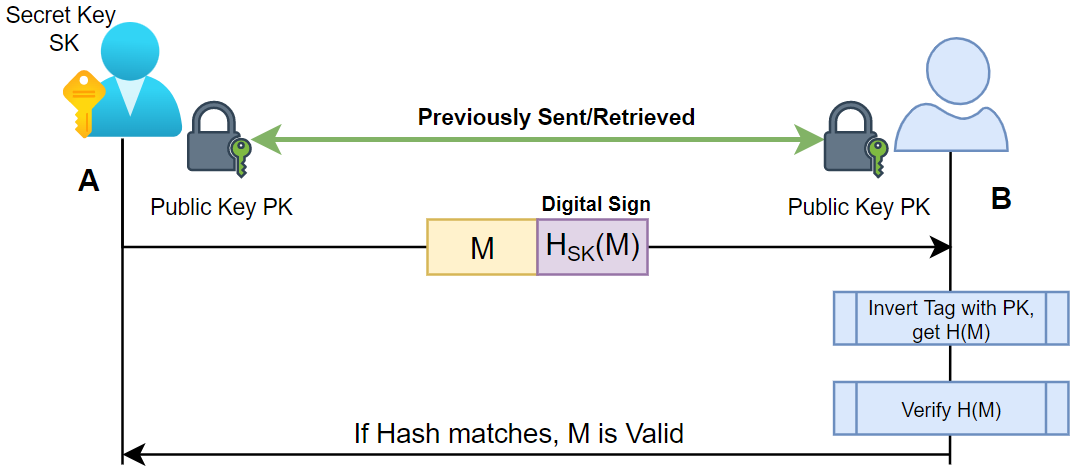
\includegraphics{image/digitalsign.png}
    \caption{Simple digital sign scheme}
    \label{fig:digitalsign}
\end{figure}
La firma digitale permette di avere un sistema più sicuro rispetto ad un semplice tag, in quanto siamo \textbf{certi} che chi ha firmato il documento è il vero autore. Difatti, in crittografia simmetrica, non è possibile dedurre l'autore del messaggio a partire dal tag, perché chiunque potrebbe produrlo. Nel caso della digital signature, vale invece la seguente proprietà
\begin{definition} [Non-Repudiation Property]
E' un concetto di sicurezza dove viene garantita l'integrità del messaggio che viene trasmesso, fornendo un identificatore per l'autore della firma.
\end{definition}

\section{Key Agreement Algorithms}
Il problema fondamentale di un meccanismo a chiave asimmetrica è che è necessario sviluppare un modo per condividere le chiavi ed instaurare il processo di \textit{Key Agreement}, ovvero un punto nel protocollo nel quale vengono fissate le chiavi da usare per scambiare i messaggi.\\
Supponiamo di suddividere la chiave $K$ in due parti $k_1,k_2$, allora il problema di ricostruire la chiave è facile se le due parti sono remark, ma è difficile data la chiave capire quali sono le parti che la costituiscono. Gli algoritmi principali di key agreement sono due: RSA e Diffie-Hellman.\\
Un attaccante che vuole trovare la chiave in un sistema che usa questi algoritmi è di fronte a due problemi:
\begin{proposition}[Discrete Logarithm Problem in Prime Field]\label{prop:disclog}
Dati tre \textbf{numeri primi \textsc{GRANDI}} $p,g,x$ \textbf{è facile calcolare}; $y=g^x\mod{p}$.\\
Dato $y=g^x\mod{p}$ \textbf{è difficile calcolare}: $x=\log_g(y)\mod{p}$
\end{proposition}
\begin{proposition}[Product Factorization of Two \textbf{Large} Prime Numbers]\label{prop:prodfact}
Dati due \textbf{numeri primi \textsc{GRANDI}} $p,q$ \textbf{è facile calcolare}: $N=p\cdot{q}$.\\
Dato $N$ è \textbf{difficile trovare} la fattorizzazione in numeri primi di $p$ e $q$.
\end{proposition}
\begin{remark}
Per \textbf{"facile/difficile"} intendiamo che esiste o meno un algoritmo per il calcolo \textbf{efficiente} di quel valore.
\end{remark}
Vediamo perché calcolare $g^x$ è facile: 
\begin{algorithm}
\caption{Square and Multiply}\label{alg:squaremult}
\begin{algorithmic}[1]
\Procedure{exp\_by\_squaring}{$g,x$}\Comment{Fast compute $g^x$}
\If {$x=0$} 
    \Return 1
\ElsIf {$x=1$} 
    \Return g
\Else
\State $exp\gets x_2[1:]$\Comment{Take exponential in base 2 and cut the msb}
\State $r\gets g$
\ForAll{$b$ \textbf{in} $exp$}\Comment{Loop from $2_{\text{nd}}$ msb to the lsb of $exp$}
    \State $r\gets r^2$\Comment{For every bit, square $g$}
    \If {$b[i]==1$}\Comment{If current bit is 1, multiply by $g$}
       \State $r\gets r\times g$
    \EndIf  
\EndFor
\EndIf
\EndProcedure
\end{algorithmic}
\end{algorithm}\\
La complessità dell'algoritmo è ovviamente $O(log_2(x))=O(n)$ per i quadrati e $O(log_2(x)/2)=O(n/2)$ per le moltiplicazioni, con $n$ numero di bit necessari a costruire l'esponente.\\
L'algoritmo rappresenta un metodo veloce per calcolare un qualsiasi esponenziale, ma lavorando con il modulo, abbiamo una sovrapposizione remarkvole di valori per il quale rende difficile il problema del calcolo inverso.\\
Vediamo un esempio grafico del perché è difficile calcolare l'inversa di un esponenziale in modulo, graficando i punti di $y=3^x\mod104729$, con $x\in\{0,3000\}$\\
Vediamo i due principali algoritmi di key-agreement.
\begin{figure}[ht]
    \centering
    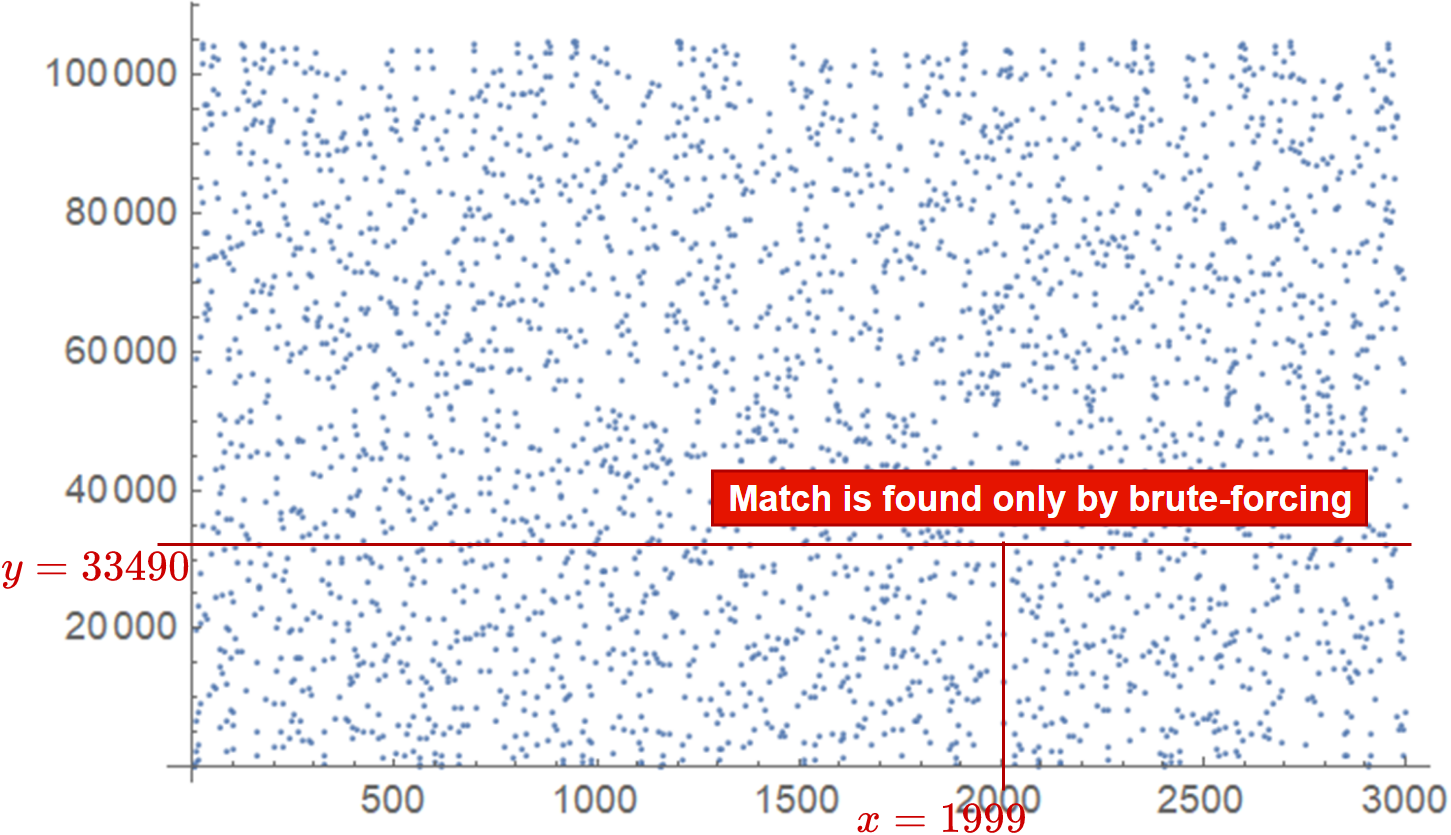
\includegraphics[width=0.7\textwidth]{image/descretelog.png}
    \caption{Descrete Logarithm Problem: How to invert the exponetial?}
    \label{fig:descretelog}
\end{figure}
\section{Diffie Hellman}
Lo scopo dell'algoritmo è \textbf{esclusivamente} lo scambio di chiavi. L'idea si basa sul calcolo dell'esponenziale in modulo dei numeri primi. Questo permette di rendere arduo il calcolo inverso. L'algoritmo lavora al seguente modo:
\begin{definition}[(Vanilla) Diffie-Hellman]\label{def:dh}
Consideriamo due utenti A, che \textbf{genera un rnd} $x$, B che \textbf{genera un rnd} $y$. \textbf{Queste sono le chiavi private degli utenti}.\\
Assumiamo che vengano precedentemente scambiati i parametri $g,p$\footnotemark{In realtà $p$ deve avere delle proprietà particolare che vedremo poi}, rispettivamente \textbf{base} dell'esponenziale e \textbf{numero primo GRANDE}.
\begin{enumerate}
    \item A invia $g^x\mod{p}$
    \item B invia $g^x\mod{p}$
    \item A calcola $K=(g^y)^x\mod{p}$
    \item B calcola $K=(g^x)^y\mod{p}$
\end{enumerate}
Adesso i due utenti hanno le chiavi necessarie.
\end{definition}
\begin{remark}Nonostante è vero che un attaccante che intercetta i due messaggi non può calcolare $g^{xy}$ con facilità, vedremo che non bisogna \textbf{MAI} usare Diffie-Hellman così come è fatto in quanto un MITM è dietro l'angolo. 
\end{remark}
\begin{remark}
DH \textbf{NON SUPPORTA} la firma digitale e lo scambio di messaggi.
\end{remark}
\subsection{Implementazioni di DH}
L'algoritmo di Key Agreement di DH è stato implementato in tre modi. Nella sua versione \textit{\textbf{Vanilla}} viene detto anche \textbf{Anonymous DH}, perché i valori $x$ e $y$ sono \textbf{generati dinamicamente} ma \textbf{non autenticati}. Tuttavia questo metodo risulta poco sicuro a fronte di attacchi MITM come possiamo vedere in \cref{fig:mitmdh}
\begin{figure}[ht]
    \centering
    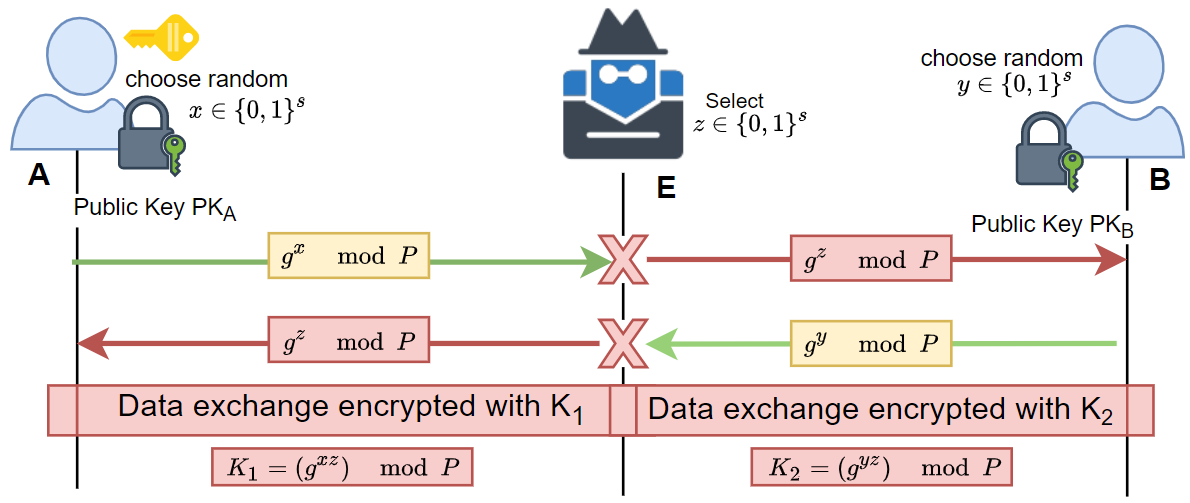
\includegraphics{image/mitmdh.png}
    \caption{MITM in DH Key Agreement}
    \label{fig:mitmdh}
\end{figure}\\
Se i messaggi fossero stati autenticati tramite firma, questo non sarebbe successo.
Per sopperire a questa vulnerabilità abbiamo due implementazioni aggiuntive: 
\begin{definition}[Fixed DH]\label{def:fixdh}
A genera un numero $x$, B un numero $y$. Vengono allora calcolati rispettivamente $g^x\mod(P)$ e $g^y\mod(P)$.\\
I due coefficienti pubblici vengono \textbf{mantenuti statici} e \textbf{firmate} da una Certification Authority (\cref{def:ca}). A questo punto si procede con il key agreement in versione standard.
\end{definition}
\begin{corollary}[Vulnerabilites of Fixed DH]
Il segreto $g^{xy}\mod(P)$ è ora sempre lo stesso e hardcoded nel certificato, pertanto andrà \textbf{sempre usato quello} per le future connessioni fino alla sua scadenza (\cref{sssec:digitalcert}). Questo genera problemi nel caso di attacchi particolari, che sfruttano una mole di dati che si estende per un lasso temporale molto ampio (anche anni).\\
\textbf{Conseguenza:} Esposizione a \textbf{dictionary attacks}.
\end{corollary}
\begin{definition}[Ephimeral DH]\label{def:ephdh}
A genera un numero $x$, B un numero $y$. Vengono allora calcolati rispettivamente $g^x\mod(P)$ e $g^y\mod(P)$ e auto-firmati da loro stessi.
Durante il processo di scambio insieme ai coefficienti pubblici vengono inviati anche i rispettivi certificati, firmati da una CA. Vengono scambiati quindi i seguenti pacchetti:
\begin{table}[H]
    \centering
    \begin{tabular}{c c}
         \textbf{A invia}& \textbf{B invia} \\
        $(A, g^x)_{A\_sign}$ & $(A, g^y)_{B\_sign}$ \\
         $(A, PK_A)_{CA\_sign}$&$(B, PK_B)_{CA\_sign}$
    \end{tabular}
\end{table}
\begin{remark}
Questa variante permette di cambiare il coefficiente pubblico a piacere, in quanto l'identità delle entità coinvolte sarà certificata dalla CA
\end{remark}
\end{definition}
\begin{corollary}[Vulnerabilities of Ephimeral DH]
Gli \textbf{attacchi MITM} sono \textbf{bloccati} dal fatto che i \textbf{coefficienti pubblici} sono \textbf{firmati da una CA} e il coefficiente può essere generato localmente quante volte si vuole. 
\end{corollary}
\section{RSA}
Algoritmo sviluppato da \textit{Rivest, Shamir, Adleman} nel '77 e brevettato fino al 2000, RSA è tra gli algoritmi di cifratura più famosi al mondo. Si basa sul problema della fattorizzazione di numeri primi (\cref{prop:prodfact}) e sulla \textbf{modular exponentiation} per cifrare e decifrare i messaggi.
\begin{proposition}[RSA Encryption]\label{prop:rsaenc}
Dato un messaggio $m$, una \textbf{chiave pubblica} $K_{pub}$ e un numero primo \textbf{grande} $N$
\begin{equation}
    C = (m)^{K_{pub}}\mod{N}
\end{equation}
\end{proposition}
\begin{proposition}[RSA Encryption]\label{prop:rsadec}
Dato un messaggio cifrato $C$, una \textbf{chiave privata} $K_{sec}$ e un numero primo \textbf{grande} $N$
\begin{equation}
    m = (C)^{K_{sec}}\mod{N}
\end{equation}
\end{proposition}
Vediamo però un esempio:
\begin{example}
Poiché per costruzione l'algebra modulare comporta l'introduzione di un \textbf{periodo} lungo quanto il numero rispetto cui viene calcolato, $m^x\mod{N}$ è periodica e abbiamo un problema di \textbf{ciclicità}.
\begin{equation*}
    \begin{aligned}
    3^x\mod{10}&={\textcolor{red}{3,9,7,1},3,9,7,1,\dots}\\
    7^x\mod{10}&={\textcolor{red}{7,9,3,1},7,9,3,1,\dots}\\
    9^x\mod{10}&={\textcolor{red}{9,1},9,1,9,1,\dots}\\
    \end{aligned}
\end{equation*}
\end{example}
\begin{remark}
RSA supporta sia firma digitale che la cifratura.
\end{remark}
Il teorema di \textit{Eulero-Fermat} permette di calcolare il \textbf{periodo} dell'esponente modulare:
\begin{proposition}[Euler's Totient Function]
Sia $\Phi(N)=E$ il massimo periodo. Se $m,N$ sono coprimi ($GCD(m,N)=1$), allora
\begin{equation}\label{eq:eulertot}
    m^{\Phi(N)}\mod{N}=1 
\end{equation}
\end{proposition}
Calcoliamo la funzione \cref{eq:eulertot} nel caso di RSA. 
\begin{itemize}
    \item Sia $p$ un numero primo, allora $\Phi(p)=p-1$ per costruzione.
    \item Siano $p,q$ primi. Allora \[\Phi(p\cdot{q})=\Phi(p)\cdot\Phi(q)=(p-1)(q-1)\]
    \item Sia $p^k$ un numero primo, allora 
    \[\Phi(p^k)=\Phi(p)\cdot p^{k-1}=(p-1)\cdot p^{k-1}\]
    \item Generalmente, se $N=\prod_{i=1}^{z}p_i^{k_i}$, allora
    \[\Phi(N)=\prod_{i=1}^{z}(p_i-1)p_i^{k_i-1}\]
\end{itemize}
Il caso di RSA è ovviamente $Phi(p\cdot{q})$. La conseguenza della periodicità in RSA è dimostrabile con un esempio:
\begin{example}
Consideriamo $2^x\mod{11}=\{2,4,8,5,10,9,7,3,6,1\}$. Poiché $p=11$ è primo, allora $Phi(11)=10$. Supponiamo di calcolare $9\cdot7\mod11$.
\begin{itemize}
    \item \textbf{Moltiplicazioni mod11:} $9\cdot7\mod11=63\mod11=8$
    \item \textbf{Approccio alternativo:} Osserviamo che $9=2^6\mod11$ mentre $7=2^7\mod11$. Allora:
    \[9\cdot7\mod11=2^6\cdot2^7\mod11=2^{13}\mod11=2^{10+3}\mod11=1\cdot2^3\mod11=8\]
\end{itemize}
\begin{remark}
La conseguenza quindi è che se dobbiamo calcolare l'esponente ad una potenza elevata qualsiasi, possiamo calcolare direttamente $g^{x\mod\Phi(N)}\mod N$, invece di calcolare il vero esponente.
\end{remark}
\end{example}
\subsection{RSA Key Transport}
Vediamo ora come  l'algoritmo costruisce le sue chiavi.
\begin{definition}[RSA Key Generation]\label{def:rsakey}
\begin{enumerate}
    \item Generare due numeri primi \textbf{grandi}: $p,q$ che \textbf{devono restare segreti}
    \item Calcolare l'\textbf{RSA module:} $N=p\cdot q$. Questo \textbf{numero} è reso \textbf{pubblico}.
    \item Calcolare $\Phi(N)=(p-1)(q-1)$, che \textbf{deve restare segreto}.
    \item \textbf{Generare una chiave pubblica} $e$ che sia \textbf{coprima con $\Phi(N)$}. Ovvero: 
    \[1<e<\Phi(N)\]
    \item \textbf{Generare una chiave privata} $d$ tale che
    \[e\cdot d=1\mod\Phi(N)\]
    \[d=e^{-1}\mod\Phi(N)\]
\end{enumerate}
\begin{remark}
Generare una private-key in questo modo è possibile \textbf{se solo se} $e$ è invertibile in $\mod(\Phi(N))$, per questo serve che siano \textbf{coprimi}. Se $\Phi(N)$ \textbf{è segreto}, è ovviamente difficile calcolare $d$ partendo da $e$.
\end{remark}
\end{definition}
Vediamo l'effetto di questa generazione delle chiavi:
\[C=M^e\mod N\]
\[M=C^d\mod N=(M^e)^d\mod N=M^{ed}\mod N=M^1\mod N = M\]
\begin{definition}[Algoritmo di Euclide Esteso]\label{def:exteuclid}
Consideriamo l'\textbf{identità di Bézout}: Dati due interi $a,b$, allora $\exists x,y$ coefficienti tale che
\[ax+by=MCD(a,b)\]
Per trovare $x,y$, costruiamo la seguente tabella:
\begin{center}
\begin{tabular}{|c|c|c|c|}
\hline
    x & y & r & q \\
\hline
    $1$ & $0$ & $\max\{a,b\}$& - \\ 
\hline
    $0$ & $1$ & $\min\{a,b\}$& $a/b$\\
 \hline
    \dots&\dots&\dots&\dots\\
\hline
    $x_{i-2}-r_{i-1}\cdot{x_{i-1}}$&$y_{i-2}-r_{i-1}\cdot{y_{i-1}}$&
    $rest(q_{i-2}/q_{i-1})$&$q_{i-2}/q_{i-1}$\\
\hline
    \dots&\dots&\dots&\dots\\
\hline
    $x^*$&$y^*$&$1$&-\\
\hline
\end{tabular}
\end{center}
I coefficienti cercati sono nell'ultima riga della tabella, che conterrà tante righe quante sono necessarie a far apparire $1$ nella colonna delle $q$. 
\end{definition}
\begin{example}[ Why RSA works?]
Supponiamo di essere in uno scenario di \textit{Decryption Challenge}: Dati $N,e$ e il messaggio cifrato $m^e$, calcolare la chiave di decifrazione (quella privata) $x$ tale che \[(m^e)^x\mod(N)=m\]
Normalmente sarebbe un problema difficile risolvere il problema perché l'unico modo è fare brute force sui possibili valori di $x$. \textbf{Se conosciamo} $\Phi(N)$ allora in tempo polinomiale è possibile trovare la soluzione della seguente equazione:
\[x=e^{-1}\mod\Phi(N)\]
\end{example}
\begin{example}[ Compute RSA Inverse]
Consideriamo uno scenario dove $e=K_{pub}=13$ e $N=77=11\times7$. Allora $\Phi(77)=10\times6=60$. Osserviamo che $MCD(e,\Phi)=1$ e quindi sono coprimi. Vogliamo calcolare la chiave privata $d$.\\
Innanzitutto calcoliamo i coefficienti $a,b$ tali che $\Phi a+eb=1$
\begin{center}
\begin{tabular}{|c|c|c|c|}
\hline
    x & y & r & q \\
\hline
    $1$ & $0$ & $60$& - \\ 
\hline
    $0$ & $1$ & $13$& $4$\\
 \hline
    $1$ & $-4$ & $8$ & $1$  \\
\hline
    $-1$ & $5$ & $5$ & $1$\\
\hline
    $-2$ & $-9$ & $3$ & $1$\\
\hline
    $-3$ & $14$& $2$&$1$\\
\hline
    $5$ & $-23$ & $1$ & -\\
\hline
\end{tabular}
\end{center}
Allora: $60\times5+13\times(-23)=1$. Per cui: $13^{-1}\mod60=-23$ e quindi $d=60-23=37$.
\end{example}
\begin{example}[ RSA toy example]
Supponiamo di applicare RSA, con $p=11,q=17,N=11\times17=187$. Abbiamo quindi la fattorizzazione in numeri primi e il numero su cui calcolare il modulo. Allora:
\[\Phi=(p-1)\times(q-1)=10\times16=160\]
Scegliamo la chiave pubblica nell'intervallo $\{1,160\}$: $e=7$. Allora:
\[d=7^{-1}\mod160=23\]
\begin{remark}
$23\times7\equiv=161=160+1=1\mod160$
\end{remark}
Abbiamo allora:
\begin{center}
    \begin{tabular}{c c}
     Enc: & $C=M^7\mod187$ \\
     Dec: & $M=(M^7)^{23}\mod187=M^{7\times23}\mod187=M$ \\
     Digital Sign: & $TAG=H(M^{23})\mod187$\\
     Verify Sign: & $H(M)=(TAG)^7\mod187=(H(M^{23}))^7\mod187$
\end{tabular}
\end{center}
Per verificare l'integrità, basta controllare che l'hash calcolato su M sia quello dedotto dalla firma.
\end{example}
\subsection{Bleichenbacher's Oracle}
\begin{definition}[Non-Malleability]
Diremo che un protocollo \textbf{non è malleabile} se, dato un messaggio cifrato $C$ di un plaintext $M$, un attaccante \textbf{NON} è in grado di creare un ciphertext differente $C'$ la cui decriptazione porta ad un messaggio $M'$ che è \textbf{in qualche modo legato} ad $M$
\end{definition}
RSA presenta un problema fondamentale, è \textbf{malleabile}. 
il protocollo di key-transport di RSA (\cref{def:rsakey}) è vulnerabile al Bleichenbacher Oracle, ovvero un attacco \textbf{Adaptive CCA}, che sfrutta la costruzione del padding in RSA, la sua \textbf{\textit{malleabilità}} ed eventuali messaggi di error signaling della \textit{specifica implementazione} del protocollo, al fine di \textbf{ricostruire il plaintext}.
\begin{definition}[Bleichenbacher's Oracle]\label{def:bleichenoracle}
Supponiamo che l'implementazione di RSA fornisca un modo per \textbf{determinare il primo bit del plaintext} $M$, generato dalla \textbf{decriptazione} all'arrivo di un \textbf{ciphertext arbitrario}\footnotemark.\\
\footnotetext{\textsuperscript{\thefootnote}Stiamo chiedendo che esista un \textbf{oracolo} di \textbf{decrittazione} solamente per il primo bit.}
L'attaccante pyuò effettuare il seguente \textbf{CCA}:
\begin{enumerate}
    \item Sia $C=M^e\mod(N)$ il \textbf{ciphertext obiettivo}.
    \item Sia $r=1$ e calcoliamo 
    \begin{equation*}
        \begin{aligned}
            C'&=((C\mod(N))\cdot(r^e\mod(N)))\mod(N)=\\
            &=(C\cdot r^e)\mod(N)\equiv(M\cdot r)^e\mod(N)
        \end{aligned}
    \end{equation*}
    \item \textbf{Inviamo} al sistema $C'$ per farlo \textbf{decifrare}. Per l'assunzione iniziale \textbf{otteniamo} il \textbf{primo bit} di ($M\cdot r$).\footnotemark
    \footnotetext{\textsuperscript{\thefootnote}In particolare il primo bit di $M$ coincide con quello di $M\cdot r$ se shiftato a sinistra di $log_2(\#bits_r)$}
    \item Moltiplicando per $r^{-1}$ troviamo il bit di $M$. 
    \item Ponendo $r=r\cdot2$ possiamo ripetere il processo e scoprire tutto $M$
\end{enumerate}
\end{definition}
\begin{remark}
Con un bleichenbacher oracle servono al più $log_2(n)$ tentativi per decifrare $M$. con $n=log_2(M)$bits
\end{remark}
\section{Pub-Key Infrastructure}
Consideriamo uno scenario di key agreement (scambio di chiavi pubbliche e setup di chiavi private comuni per creare un canale sicuro). Fino ad ora non ci siamo preoccupati di verificare la validità della chiave pubblica rilasciata da un utente e l'abbiamo solo usata per decifrare il tag aggiunto al messaggio per ottenere l'hash di $M$ nel caso della firma digitale, oppure per stabilire una chiave comune per la cifratura del canale di comunicazione con RSA. 
\begin{figure}[ht]
    \centering
    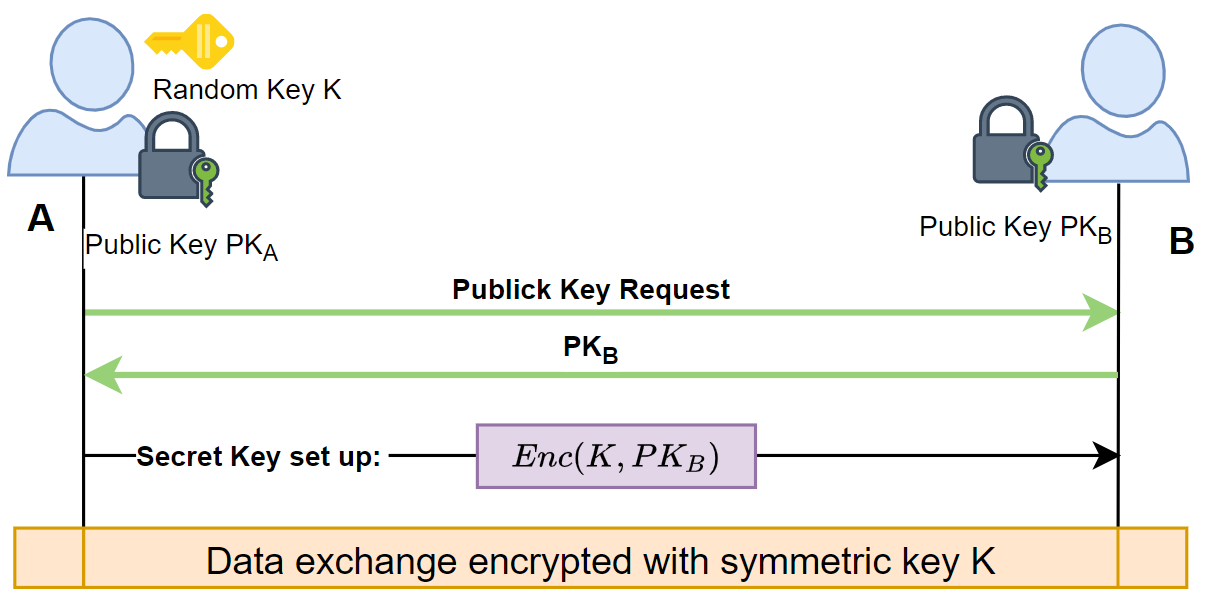
\includegraphics[width=\textwidth]{image/rsakeytrans.png}
    \caption{RSA Key Transport}
    \label{fig:rsakeytrans}
\end{figure}
\begin{remark}Se un attaccante rispondesse alla richiesta di un utente di scaricare una chiave pubblica e la sostituisse con la propria, allora ogni messaggio inviato da quel momento in poi dall'attaccante sarebbe considerato valido perché la public key è stata sostituita. 
\end{remark}
Vediamo lo schema di un possibile attacco ad RSA:
\begin{figure}[ht]
    \centering
    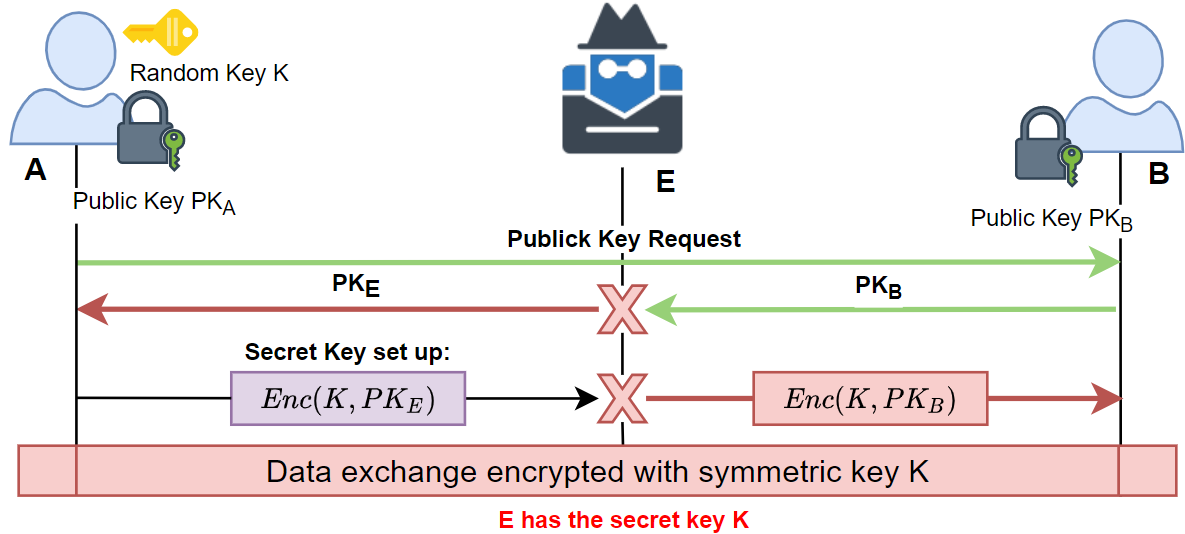
\includegraphics{image/mitmrsa.png}
    \caption{MITM in RSA Key Transport}
    \label{fig:mitmrsa}
\end{figure}\\
\begin{remark}
Diffie-Hellman non avrebbe comunque protetto da questo tipo di MITM, vedi \cref{fig:mitmdh}
\end{remark}
\begin{proposition}
Per scambiare le chiavi \textbf{è necessario} legare in \textbf{modo crittografico} la \textbf{chiave pubblica} all'\textbf{identità}.
\end{proposition}
Abbiamo bisogno di un'infrastruttura che, oltre a definire lo scambio di chiavi, definisca \textbf{protocolli}, \textbf{strategie} e \textbf{meccanismi} affinché \textbf{lo scambio sia sicuro}
\subsection{Digital Certificate}\label{sssec:digitalcert}
Un modo per essere sicuri della chiave pubblica rilasciata da un utente è quella di \textbf{fidarsi di un'entità terza}, detta \textbf{Certification Authority}, che garantisce l'integrità del legame che c'è tra la chiave e l'identità.
\begin{definition}[Certification Authority]\label{def:ca}
Una CA è una \textbf{Trusted Third Party} a cui altre entità si affidano per ricevere dei certificati di affidabilità.
\end{definition}
\begin{remark}
Una soluzione più semplice sarebbe quella di fare in modo che tutti conoscano le chiavi pubbliche degli utenti con i quali si vuole comunicare, ma questa soluzione \textbf{non è} ovviamente \textbf{scalabile}.
\end{remark}
\begin{remark}
I certificati digitali non risolvono il problema, perché potrebbe esserci un modo di falsificarli.
\end{remark}
Il modo con cui una CA rilascia un certificato è il seguente:
\begin{proposition}[Emissione di un Certificato]
Un'entità verifica \textbf{(e.g. offline)}, presso una CA, la sua identità. Vengono svolte le seguenti operazioni:
\begin{enumerate}
    \item L'entità genera una $PK$ e una $S_K$, che viene \textbf{mantenuta segreta}.
    \item L'entità comunica la sua $PK$ alla CA tramite un \textbf{canale sicuro}
    \item La CA fa le verifiche del caso e se passano tutte emette un \textbf{certificato firmato}:
    \[cert=(name_{entity}, PK)_{CA\_sign}\]
\end{enumerate}
\end{proposition}
Il modo con cui un utente si accerta che un certificato è autentico è il seguente:
\begin{definition}[Verifica della Validità di un Certificato]\label{def:certval}
Un'entità $A$ vuole accertarsi che il \textbf{certificato} di $B$ sia corretto e di \textbf{sua proprietà}. Vengono svolte le seguenti operazioni:
\begin{enumerate}
    \item A contatta B e ne \textbf{richiede} il \textbf{certificato}.
    \item B invia ad A la tripla: $\{name_B, PK_B, CERT_B\}$, dove \[CERT_B=(name_B. PK_B)_{CA\_sign}\]
    \item A verifica che $CERT_B$ sia stato emesso da una \textbf{CA fidata} per lui e che la \textbf{firma sul certificato} sia corretta.
    \item A si accerta dell'\textbf{identità} di B con una procedura "\textbf{chap-like}" (\cref{fig:chap}) in uno dei modi seguenti:
    \begin{itemize}
        \item \begin{enumerate}
        \item A invia una nonce a B
        \item B risponde ad A \textbf{firmando} la \textbf{nonce} con la \textbf{sua chiave segreta} $SK_B$.
    \end{enumerate}
    \item \begin{enumerate}
        \item A invia una challenge contenente una cifratura a B
        \[Chall=Enc(nonce)_{PK_B}\]
        \item B risponde ad A con la nonce ottenuta decifrando la challenge con la sua $SK_B$ 
        \[nonce = Dec(Chall)_{SK_B}\]
    \end{enumerate}
    \end{itemize}
\end{enumerate}
\end{definition}
\begin{remark}
Il metodo chap-like per verificare l'identità dell'entità con cui vogliamo collegarci è \textbf{necessario} per evitare replay attack sul certificato.
\end{remark}
Le CA sono molte e dislocate in tutto il mondo, organizzate poi in una struttura gerarchica. Un'architettura PKI definisce proprio queste relazioni e anche gli standard a cui i certificati devono aderire. Un esempio di certificato è il seguente:
\begin{example}[ Certificate X.509 (High Level View)]
\begin{itemize}
    \item \textbf{Versione Standard:} Indica la versione del certificato.
    \item \textbf{Validità Temporale:} Data di inizio e fine validità.
    \item \textbf{Numero Seriale:} Identificatore univoco del certificato.
    \item \textbf{Algoritmi:} Algoritmi crittografici supportati dal certificato. Detta anche \textbf{Cipher Suite}
    \item \textbf{Identità CA:} Nome della CA che ha emesso il certificato.
    \item \textbf{Identità Utente:} nome dell'utente associato al certificato.
    \item \textbf{Chiave Pubblica Utente:} chiave pubblica dell'utente.
    \item \textbf{Firma Digitale:} firma del certificato generata dalla CA.
\end{itemize}
\begin{remark}[X.509v3 Extension]
\textbf{Estensioni:} (se X.509v3) campo addizionale che può contenere diversi tipi di attributi e permette di espandere il certificato con nuove feature.
\end{remark}
\end{example}
\begin{figure}[h]
    \centering
    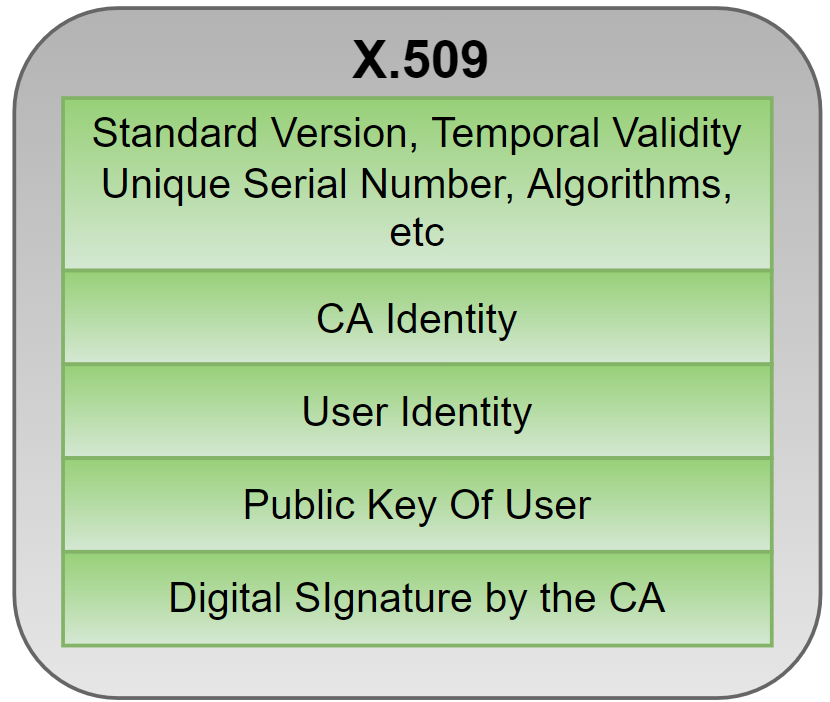
\includegraphics[width=0.48\textwidth]{image/x509.png}
    \caption{Certificate X.509}
    \label{fig:certx509}
    \vspace{-7pt}
\end{figure}
\subsection{Certificate Revocation List}
Ogni PKI \textit{\textbf{deve}} includere un meccanismo di \textit{revoca} dei certificati, poiché questi possono essere \textbf{compromessi}. Ad esempio: 
\begin{itemize}
    \item La chiave privata è stata persa o divulgata.
    \item La chiave pubblica è obsoleta e non più utilizzata.
    \item Il certificato è scaduto.
\end{itemize}
Esistono 2 approcci per la revoca di un certificato:
\begin{itemize}
    \item \textbf{Revocazione Implicita:} avviene se il \textbf{periodo di validità} di un certificato si esaurisce.
    \item \textbf{Revocazione Esplicita:} avviene quando effettuata per \textbf{\textit{Certificate Revocation List}}
\end{itemize}
\begin{definition}[Certificate Revocation List]
Una CRL è una lista mantenuta da \textbf{OGNI} CA, che periodicamente \textbf{deve} essere \textbf{aggiornata} con i certificati che la CA ha \textbf{rimosso}.\\
Possiede il seguente formato:
\begin{itemize}
    \item \textbf{Emittente (Issuer):} Indica la CA che ha \textbf{pubblicato} la lista.
    \item \textbf{Ultima Data di Aggiornamento:} ultima data in cui la lista è stata modificata.
    \item \textbf{Prossima Data di Aggiornamento:} data futura in cui verrà pubblicato il prossimo aggiornametno. Indica il periodo di validità della lista.
    \item \textbf{Elenco dei Seriali Revocati:} indica i numeri seriali dei \textbf{certificati da revocare}.
    \item \textbf{Elenco della Data di Revocazione}.
    \item \textbf{Firma Digitale:} firma generata dalla CA emittente della lista.
\end{itemize}
\end{definition}
\begin{remark}
Ogni entità che utilizza un certificato \textbf{dovrebbe sempre verificarne la validità} controllando la relativa CRL. Tuttavia, questa operazione è demandata ad applicazioni che svolgono un ruolo \textbf{critico} nella rete, per alleggerire il carico complessivo.
\end{remark}
\subsection{Public Key Criptography Standards}
La PKI specifica molti aspetti legati alla \textbf{crittografica asimmetrica}. Gli standard sono definiti dalle:
\begin{definition}[PKCS]
Public Key Criptography Standards
\end{definition}
Attualmente vanno dal numero 1 al numero 15, alcuni di questi sono: 
\begin{itemize}
    \item \textbf{PKCS\#1:} RSA
    \item \textbf{PKCS\#3:} DH
    \item \textbf{PKCS\#6:} Estensione del formato \textbf{X.509}. Alcune delle estensioni più comuni sono:
    \begin{proposition}[X.509 Extensions]
    \begin{itemize}
        \item \textbf{Authority Key Identifier:} identifica la chiave pubblica corrispondente alla chiave privata \textbf{usata per firmare un certificato}.
        \item \textbf{Subject Key Identifier:} Identifica i certificati che contengono al loro interno una determinata chiave pubblica.
        \item \textbf{Key Usage:} Specifica lo scopo della chiave contenuta nel certificato. Ovvero, per quale meccanismo può essere utilizzata.
        \item \textbf{Subject Alternative Name:} permette di associare più identità al soggetto del certificato, che possono aggiungersi o rimpiazzare le precedenti.
        \item \textbf{Extended Key Usage:} Specifica ulteriori scopi per la chiave pubblica contenuta nel certificato. che ossono aggiungersi o rimpiazzare quello specificato nell'estensione precedente.
    \end{itemize}
    \end{proposition}
    \item \textbf{PKCS\#10:} \textbf{CRSS (Certification Request Syntax Standard)}. Specifica il formato dei messaggi di richiesta dei certificati. Un esempio è il seguente:
    \begin{proposition}[Certification Signing Request - CSR]
    Messaggio inviato da parte di una CA al fine di \textbf{applicarsi per un certificato} della \textbf{sua identità digitale}. Le operazioni svolte dall'applicante sono:
    \begin{enumerate}
        \item Genera una coppia di chiavi, pubblica e privata. L'ultima viene mantenuta segreta.
        \item Genera un \textbf{CSR}, contenente le informazioni per identificarsi: Nome, Chiave pubblica e, eventualmente, alcune estensioni.
        \item Il \textbf{CSR} viene \textbf{inviato} \textbf{insieme} ad \textbf{altre credenziali} o \textbf{prove di identità} richieste dalla CA. Inoltre, quest'ultima può contattare l'applicante per richiedere ulteriori informazioni.
    \end{enumerate}
    \end{proposition}
    \item \textbf{PKCS\#11:} \textbf{CTIS (Cryptographic Token Interface Standard)}. Specifica l'API per \textbf{firmare e verificare} dati da parte di un dispositivo che mantiene chiavi.
    \item \textbf{PKCS\#12:} \textbf{PIESS (Personal Information Exchange Syntax Standard)}. Specifica il \textbf{formato} dei file utilizzati per \textbf{memorizzzare i certificati} e le \textbf{chiavi private} usati per spostare informazioni riservate tra diversi browsers.
    \item \textbf{PKCS\#13:} \textbf{ECC (Elliptic Curve Cryptography)}
\end{itemize}
\subsection{Certificate Chains}
Per distribuire le responsabilità e il carico delle certificazioni digitali, le CA vengono \textbf{organizzate} secondo una \textbf{gerarchia ad albero} dove i nodi radice sono considerati, per definizione, i più sicuri.\\
L'ovvio problema di questa struttura gerarchica è che, eccezion fatta per la radice, \textbf{non abbiamo garanzie} che un particolare nodo dell'albero sia \textbf{trusted}, ovvero che a sua volta la sua identità sia verificata. Sono necessari dei meccanismi aggiuntivi, detti proprio \textbf{certificate chains}.\\
\begin{remark}
I meccanismi aggiuntivi sono \textbf{necessari} in quanto su una singola macchina non è possibile salvare tutti i certificati di tutto il mondo, serve qualcosa di scalabile, come un database distribuito.
\end{remark}
\begin{definition}[Certificate Chain]
Una catena è una lista di certificati seguiti da una o più CA, con le seguenti proprietà:
\begin{itemize}
    \item L'entità che rilascia il certificato è collegata alla prossima in lista. 
    \item \textbf{Ogni} certificato, a parte l'ultimo, è firmato dalla chiave segreta corrispondente al prossimo certificato nella catena.
    \item L'\textbf{ultimo} certificato in lista è un \textbf{trust anchor}, del quale l'utente si fida perché gli è stato fornito tramite una procedura attendibile. Dalle trust anchor inizia il processo di validazione.
\end{itemize}
\end{definition}
Una delle estensioni che è possibile trovare nel certificato è la seguente:
\begin{theorem}[Basic Constraint]\label{thm:basiccons}
E' un valore booleano, che indica se il l'entità legata a al certificato ha o meno il permesso di utilizzare la propria chiave privata per firmare altri certificati.
\end{theorem}
\begin{remark}
Permette di individuare un certificato illegittimo nella catena.
\end{remark}
\begin{remark}
Una compagnia può avere un cosiddetto \textbf{Wildcard Certificate}. E' un certificato jolly, che permette di certificare tutti i suoi sistemi, con nome diverso, in uno stesso dominio.
\end{remark}
Il meccanismo di certificazione è simile a quello espresso in \cref{def:certval}, ma questa volta c'è almeno un nodo intermedio in più.
\begin{definition}[Certificate Chain Procedure]\label{def:certchain}
Supponiamo che A voglia autenticare B. Supponiamo che \textbf{$CA_B$} sia la certificante di B e che $U$ sia la root della catena di certificazione di B ma che sia nella lista delle CA \textbf{universalmente verificate} di A.
\begin{enumerate}
    \item B invia ad A il suo certificato che A controllerà per individuare la validità e, \textbf{soprattutto}, la CA che lo firma. Abbiamo due casi: 
\begin{itemize}
    \item \textbf{La CA di B è nella lista di A:} B è certificata.
    \item \textbf{La CA di B NON è nella lista di A:} Servono ulteriori certificati.  
\end{itemize}
\item B richiede alla sua CA il suo certificato, che inoltra ad A.
\item A vede che il certificato di $CA_B$ è del tipo: \[(CA_B, PK_{CA_B})_{U_{sign}}\]
E poiché \textbf{U è nella sua tabella e universalmente verificata}, B è verificata.
\end{enumerate}
\end{definition}
\begin{remark}
Tipicamente non va sempre così: sono necessari diversi certificati per risalire fino ad una CA effettivamente nella lista di A. In quel caso vengono inviati ad A tutti i certificati intermedi, per poter ricostruire la catena. 
\end{remark}
\subsection{Merkel's Tree}
Consideriamo per un momento il problema di garantire l'integrità di un file. 
\begin{proposition}[Best Practices for Integrity]\label{prop:bestpractint}
Per garantire l'integrità di un file in maniera efficiente occorre provvedere a due aspetti:
\begin{enumerate}
    \item \textbf{Generare} una \textbf{segnatura (fingerprint)} del file \textbf{H(file)} con una funzione cryptho-hash \textbf{H}.
    \item \textbf{Proteggere} la \textbf{segnatura} in uno dei seguenti modi:
    \begin{itemize}
        \item \textbf{Memorizzare} la fingerprint in uno \textbf{spazio di archiviazione sicuro} (una chiavetta, disco rimosso dalla rete ecc).
        \item \textbf{Generare} la \textbf{firma digitale del file} $H(file)_K$.
        \begin{remark}
            Firmare il file da proteggere o il suo hash è equivalente perché l'hash preserva il contenuto del file da un punto di vista dell'integrità
        \end{remark}
    \end{itemize}
\end{enumerate}
\end{proposition}
Come comportarsi però quando il \textbf{file} da proteggere è \textbf{troppo grande} e deve essere \textbf{scomposto} in diversi \textbf{blocchi (chunk)}? Sono chiaramente necessarie due operazioni per garantire quanto affermato in \cref{prop:bestpractint}:
\begin{itemize}
    \item \textbf{Verifica Indipendente} della \textbf{segnatura} dei \textbf{singoli chunk}. La verifica indipendente è necessaria poiché i chunks possono essere ricevuti fuori ordine e da mittenti differenti.
    \item \textbf{Verifica} della \textbf{segnatura} dell'\textbf{intero file} riassemblato alla fine della ricezione, \textbf{per impedire attacchi ai singoli chunk} sfuggiti al controllo precedente.
\end{itemize}
Al fine di applicare queste soluzioni, abbiamo due approcci:
\begin{itemize}
    \item \textbf{Hash dell'Intero File:} si genera un unico digest per il file. Allora:
    \begin{itemize}
        \item [\textcolor{red}{\ding{55}}]Serve che \textbf{tutti} i \textbf{chunk} sia stati ricevuti per ricostruire il file e poi produrre il digest.
        \item [\textcolor{red}{\ding{55}}]La \textbf{verifica} di un \textbf{singolo chunk} può essere fatta \textbf{solo se} si \textbf{possiedono} tutti \textbf{gli altri}
        \item [\textcolor{red}{\ding{55}}]Un attaccante può \textbf{inserire chunk malevoli} durante l'invio. \textbf{(fake chunk injection)}
    \end{itemize}
    \item \textbf{Hash di ogni chunk:} per ogni chunk genero un \textbf{tag}. Allora:
    \begin{itemize}
        \item [\textcolor{red}{\ding{55}}]\textbf{Grande spreco} di risorse computazionali e di archiviazione.
        \item [\textcolor{red}{\ding{55}}]L'\textbf{intero file non} è più \textbf{verificabile}.
        \item [\textcolor{red}{\ding{55}}]Un attaccante può \textbf{rimuovere chunk} dal canale di comunicazione. \textbf{(Strip-type attacks)}
    \end{itemize}
\end{itemize}
Tali problematiche non sussistono se utilizziamo una struttura dati ad-hoc.
\begin{definition}[Merkle's Hash Trees]
Un Merkle Tree è un albero binario i cui nodi interni sono costituiti da hash di chunk di un file e le foglie sono i chunk stessi. Per ogni nodo, tranne la radice, identifichiamo dei \textbf{siblings}, ovvero l'insieme dei fratelli ad ogni livello superiore al nodo considerato.\\
Questa costruzione permette di creare una fingerprint per singolo chunk che garantisce di:
\begin{itemize}
    \item Verificare l'integrità utilizzando \textbf{solamente i siblings} che si incontrano lungo il cammino dalla foglia alla radice dell'albero.\\
    \begin{remark}
    Servono \textbf{solo} i $\log_2(N)$ tag presenti nei nodi \textbf{opposti} ad uno stesso livello dell'albero fino alla root, che viene ricostruita man mano che si sale.
    \end{remark}
    \item Verificare l'integrità dell'intero file \textbf{ricalcolando} il \textbf{tag} posto nella \textbf{root}, utilizzando ogni chunk. 
\end{itemize}
\end{definition}
\begin{example}[ $C_2$ Sign verify]
Supponiamo di voler verificare l'integrità del chunk 2 in \cref{fig:merkletree}. L'entità che esegue la verifica si fa inviare dal CTDB \textbf{tutti} i siblings necessari insieme al certificato e alla root, in questo caso sono necessari: $S_1=H(c_1),\,S_2=H(H(c_3),H(c_4))$.\\
L'entità calcola allora $H(H(c_1),H(c_2))$, con il quale a partire da $S_2$ può calcolare la \textbf{sua versione della root}. Se questa coincide con quella ricevuta dal CTDB allora $c_2$ è integro.
\end{example}
\begin{definition}[Merkle's Tree Time extension]
Un merkle tree può essere \textbf{esteso} introducendo il concetto di \textit{tempo}, usando uno schema ricorsivo nel quale alla root di un albero \textit{i-esimo} costruito al tempo $t$ associamo un altra root di un albero $j-esimo$ \textbf{costruito al tempo \textit{t$+1$}} e creiamo una root a livello $(i-1)$-esimo contenente l'hash delle due root.
\end{definition}
\begin{figure}[ht]
    \centering
    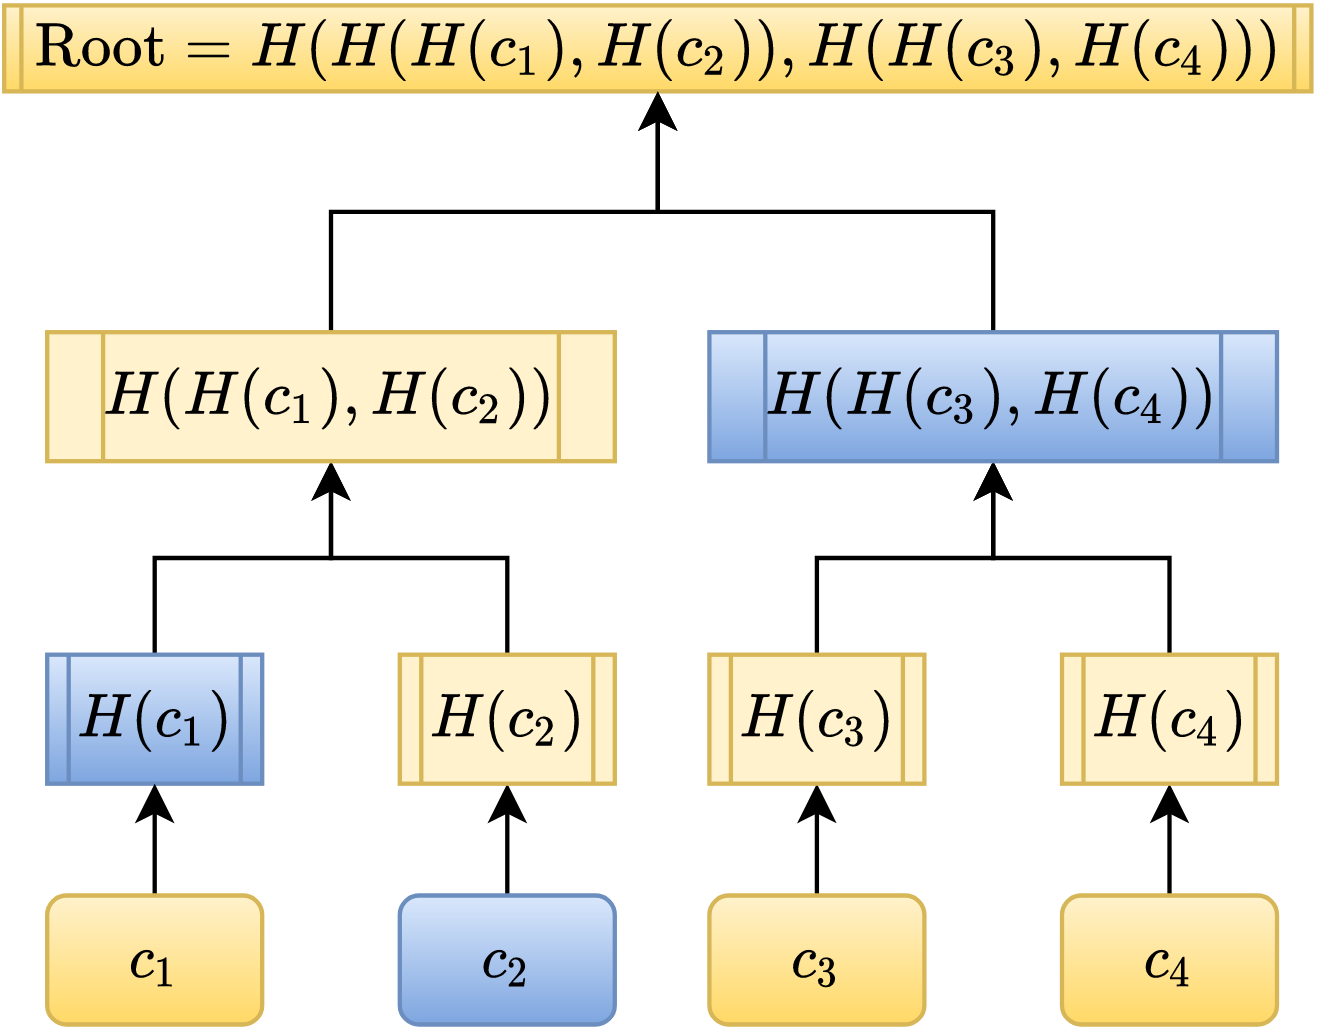
\includegraphics[width=0.4\textwidth]{image/merkletree.png}
    \definecolor{myColor1}{HTML}{7EA6E0}
    \caption{Merkle Tree example. \textbf{\textcolor{myColor1}{$c_2$'s siblings}}}
    \label{fig:merkletree}
\end{figure}
\begin{figure}[ht]
    \centering
    \includegraphics[width=0.9\textwidth]{image/merkletime.png}
    \caption{Merkle Tree with Time}
    \label{fig:merkletime}
\end{figure}
E' immediato dedurre che per verificare l'integrità di un chunk con un albero esteso servono:
\begin{proposition}[Integrity check wiht Time Extension]
\begin{itemize}
    \item I siblings dell'albero a cui appartiene il chunk.
    \item La radice dello slot temporale precedente.
    \item Le radici di tutti gli slot temporali successivi.
\end{itemize}
\end{proposition}
\begin{remark}
E' interessante notare come i merkle tree estesi permettano di costruire un sistema di \textbf{blockchain} per la verifica di certificati.
\end{remark}
\subsection{Certificate Transparency}
Il \textbf{processo} descritto nella \cref{def:certchain} è \textbf{debole} ad attacchi, perché \textbf{se un nodo} della catena \textbf{contiene} un \textbf{certificato falso}, allora il \textbf{sistema di autenticazione} è stato \textbf{rotto} a prescindere. Inoltre, \textbf{bisogna assicurarsi} che \textbf{la CA nella nostra lista possa rilasciare certificati}, come detto in \cref{thm:basiccons}.\\
Il problema descritto precedentemente può essere formalizzato così:
\begin{definition}[Fake Certificates Problem]
Una \textbf{CA intermedia} può generare \textbf{certificati malevoli} visti però come \textbf{validi} dalle entità, \textbf{compromettendo} i \textbf{meccanismi} di \textbf{autenticazione} e \textbf{recupero} delle chiavi pubbliche nella PKI.
\end{definition}
La soluzione venne proposta da Google nel 2013 e costituisce una mitigazione del problema, perché in ogni caso c'è una debolezza intrinseca alla base dell'infrastruttura.
\begin{remark}
Se una delle entità universalmente fidate (es. Governi) dovesse, per qualche motivo, generare certificati malevoli non potremmo accorgerci di niente.
\end{remark}
L'idea è quella di creare un DB scalabile globalmente distribuito.
\begin{multicols}{2}
\begin{definition}[CTDB]
Le caratteristiche del CTDB sono:
\begin{itemize}
    \item E' \textbf{globale, scalabile e sicuro} (non modificabile a posteriori).
    \item Può essere \textbf{amministrato} da \textbf{diversi stakeholders}.
    \item Tutte le CA possono inserire nel CTDB i certificati da loro emessi.
    \item Tutte le entità e le CA possono accedere e consultare il CTDB.
\end{itemize}
\end{definition}

\columnbreak
\begin{figure}[H]
    \centering
    \includegraphics[width=0.4\textwidth]{image/certtrans.png}
    \caption{Certificate Transparency DB}
    \label{fig:certrans}
\end{figure}
\end{multicols}

Per soddisfare i requisiti funzionali il database è mantenuto in un \textbf{log server} (\textbf{unico e globalmente accessibile}), protetto
con uno schema derivante dai \textbf{Merkle's Tree esteso}, detto \textbf{Chron Tree}, caratterizzato dalle seguenti proprietà:
\begin{proposition}[Chron Tree Properties]
\begin{itemize}
    \item \textbf{Ogni certificato corrisponde ad un chunk}. Inoltre, ad ognuno di questi è aggiunto un \textbf{timestamp} per \textbf{evitare} l'\textbf{inserimento retroattivo} di certificati
    \item \textbf{L'albero è di tipo Append Only:} l'albero viene \textbf{esteso} ogni \textbf{24 ore} con un sottoalbero per la verifica della firma di tutti i certificati emessi dall'ultima estensione.
    \item \textbf{Consistency Proof:} ogni versione \textbf{successiva} del Merkle Tree \textbf{contiene per intero} la precedente come sottoalbero. Ciò rende \textbf{impossibile} la modifica di un certificato passato o l'inserimento di un \textbf{certificato retrodatato}.
    \item La verifica per un certificato necessita solamente del certificato stesso e dei siblings-tag all'interno dell'albero.
\end{itemize}
\end{proposition}
Le entità in gioco nel sistema descritto da \cref{fig:certrans} possono eseguire le seguenti operazioni:
\begin{proposition}[What a Requesting Entity can do]
Prima di utilizzare il certificato di un'entità B, l'entità richiedente A effettua i seguenti controlli:
\begin{enumerate}
    \item \textbf{Controlla} se il certificato digitale è \textbf{affidabile} tramite \textbf{certificate chain} e se è \textbf{valido}.
    \item\textbf{ Autentica B con un meccanismo CHAP-like}: A sottopone a B una \textbf{prova per la verifica della conoscenza la chiave privata} legata alla\textbf{ chiave pubblica nel certificato}.
    \item \textbf{Verifica che il certificato sia presente nel CTDB}: ricostruisce il tag root del sottoalbero del Merkle Tree esteso alla quale appartiene il certificato usando i siblings contenuti nel SCT (ricevuto insieme al certificato) e verifica la congruenza con quello presente nel log server.
    \item \textbf{Verifica che il certificato non sia presente in nessuna CRL delle CAs coinvolte.}
\end{enumerate}
\end{proposition}

\begin{proposition}[What a CA can do]
\begin{itemize}
    \item \textbf{Emettere un Certificato e Caricarlo nel CTDB}. In particolare vengono eseguite le seguenti operazioni:
    \begin{enumerate}
        \item La CA genera un \textbf{precertificato} temporaneo che invia al log-server.
        \item Il \textbf{log-server genera}, a partire dal precertificato, il relativo \textbf{certificato definitivo} e lo invia alla CA, \textbf{isieme} ad un \textbf{SCT (Signed Certificate Timestamp)}\footnotemark.
        \item La CA riceve la coppia \textbf{\{certificato, SCT\}} e la inoltra all'entità per la quale è stata generata. Per robustezza, sia CA che l'entità \textbf{mantengono localmente} il certificato e l'SCT.
        \footnotetext{\textsuperscript{\thefootnote}l'SCT contiene info aggiuntive necessarie alla verifica della validità del certificato, tra cui i siblings del sottoalbero a cui appartiene.}
    \end{enumerate}
    \item \textbf{Consultare il CRDB\footnotemark} alla ricerca di certificati malevoli emessi a suo nome, così da \textbf{inserirli} nella sua \textbf{CRL} ed ottenerne la revocazione.
    \footnotetext{\textsuperscript{\thefootnote}Certificate Revocation DB}
\end{itemize}
\end{proposition}

Il sistema di certificate transparency non è completamente primo di vulnerabilità. In particolare una CA intermedi corrotta a favore di un'entità B (non richiedente) potrebbe:
\begin{itemize}
    \item \textbf{Non aggiungere il certificato falso nel CTDB.} Tuttavia, l’entità A nota che il certificato per B non è presente del CTDB, e lo scarta a priori. \textbf{ L’attacco è perciò completamente neutralizzato.}
\item \textbf{Aggiungere un certificato falso/rubato nel CTDB.} Tuttavia, la CA proprietaria dell’identità rubata si accorgerebe subito del certificato falso inserito nella CTDB e lo aggiunge alla propria CRL.\\
L’\textbf{attacco} è perciò \textbf{mitigato}, in quanto può \textbf{esistere una finestra temporale} in cui il \textbf{certificato falso è nella CTDB ma non nella CRL}.
\end{itemize}
\begin{remark}
La ceritificate transparency è diversa da un sistema a blockchain, sebbene siano entrambe protette da merkle tree. La differenza sta nel fatto che nelle \textbf{blockchain} le \textbf{transazioni} (i chunk) sono \textbf{vere se appartengono alla blockchain}.\\
Anche se è vero che un certificato viene considerato \textbf{falso} \textbf{se non appartiene} al CTDB, questo \textbf{può} ancora \textbf{essere falso} in quanto potrebbe esser stato \textbf{revocato} da una CA ed \textbf{appartenere} ad una \textbf{CRL}.
\end{remark}

\section{Authentication with Asymmetric Crypto}
Nel contesto della \textbf{comunicazione} sicura \textbf{basata sulla crittografia asimmetrica} e i \textbf{certificati digitali}, un’\textbf{entità} \textbf{può autenticarsi} dimostrando di conoscere la \textbf{chiave privata associata alla chiave pubblica} dichiarata all'interno del suo certificato. Esistono 2 diversi approcci:
\begin{itemize}
    \item \textbf{Firma Digitale}: il sistema autenticato dimostra la conoscenza della chiave privata generando la firma digitale per una challenge composta sia da una nonce che da testo arbitrario.
    \item \textbf{Decriptazione}: Il sistema autenticato dimostra la conoscenza della chiave privata, decriptando una challenge composta sia da una nonce che da un testo arbirario. La decriptazione può avvenire in due modi:
    \begin{itemize}
        \item \textbf{Asimmetrica:} Il sistema autenticato invia solamente la challenge criptata asimmetricamente.
        \item \textbf{Simmetrica con chiave di Sessione:} l'autenticatore invia una chiave di sessione casuale, criptata asimmetricamente e la challenge criptata simmetricamente.
    \end{itemize}
\end{itemize}
\begin{figure}[h]
    \centering
    \includegraphics{image/authasymm.png}
    \caption{Authentication with Asymm Crypto}
    \label{fig:authasymm}
\end{figure}
\chapter{TLS - Transport Layer Security}
I principali \textit{network security protocol} sono \textbf{SSH}, \textbf{SSL} (\textit{secure socket layer}), \textbf{TSL} e \textbf{IPsec}. Storicamente il primo pensato fu SSL, realizzato in diverse versioni ognuna sempre migliore, fino a quella che conosciamo oggi. Facciamo un breve recap storico:
\begin{itemize}
    \item (\textbf{1994}) SSL v1 viene sviluppato da \textit{Netscape} ma mai rilasciato.
    \item (\textbf{1995}) SSL v2 viene integrato in \textit{Netscape 1.1} e verrà successivamente rotto.
    \item(\textbf{1996}) SSL v3 vene ridisegnato dalla base da \textit{Netscape}.
    \item(\textbf{1996-1999}) TLS v1.0 viene sviluppato parallelamente a \textit{SSL} dalla \textbf{IETF}, partendo dalla sua versione 3.1. Il protocollo è basato interamente su \textit{TCP} per la parte di trasmissione e integra algoritmi di sicurezza \textbf{\textit{hardcoded}}.
    \item(\textbf{2006}) TLS v1.1 viene rilasciato e viene aggiunto il supporto a \textit{UDP}. 
    \item(\textbf{2008}) TLS v1.2 viene rilasciato per disaccoppiare i sistemi di sicurezza deboli come \textit{MD5/SHA-1} precedentemente hardcoded nel sistema. Introduce il concetto di \textit{Negotiated-PRF}, impostando come default \textit{SHA-256}.
    \item(\textbf{2018}) \textbf{TLS v1.3 viene rilasciato, costituendo un nuovo protocollo}. Vengono introdotti e ammessi solo cifratori basati su \textit{AEAD} e viene aggiunto il \textbf{\textit{Threeway-Handshake}}
\end{itemize}
\begin{note}
TLS v1.3 rimuove anche \textbf{RSA}, in quanto il modo in cui viene usato può portare a diversi problemi.
\end{note}
In ultimo è utile ricordare che:
\begin{proposition}[Livelli di Protezione]
SSL/TLS sono protocolli di protezione che vanno \textbf{sopra} lo strato di trasmissione e sotto quello applicativo. Tuttavia non vanno presi come un miglioramento alla sicurezza di TCP in quanto i servizi offerti da TLS non sono limitati al garantire un trasporto sicuro di dati e descrivono una più generale relazione point-to-point.\\
Questo significa che SSL/TLS proteggono \textbf{esclusivamente}\footnotemark il payload di un determinato pacchetto.
\footnotetext{\textsuperscript{\thefootnote}IPsec protegge invece tutto il pacchetto, sia payload che header.}
\end{proposition}\pagebreak
\section{Il Supporto Applicativo}
\begin{wrapfigure}{R}{0.5\textwidth}
\vspace{-5mm}
    \centering
    \includegraphics[width=0.5\textwidth]{image/tlsencapsulation.png}
    \caption{Port change made by TLS layer}
    \label{fig:tlsencapsulation}
\end{wrapfigure}
Quando un servizio applicativo viene standardizzato bisogna specificare una serie di parametri come \textbf{IP address} e \textbf{port number} del servizio. TLS, avendo una \textit{struttura a strati}, riesce a fornire un supporto ben strutturato a questa modalità di sviluppo poiché l'applicazione utilizza nel suo pacchetto la porta del servizio applicativo da usare (es: HTTP) mentre lo strato TLS incapsula il valore di porta specificando il valore del servizio su cui c'è sicurezza.
\begin{example}
Supponiamo di inviare un pacchetto email tramite protocollo HTTP, che usa la porta 80. Poiché il servizio di mail offerto dal protocollo SMTP usa la porta 25, l'applicazione che utilizziamo per spedire il pacchetto specificherà nell'header la porta 80 e la porta 25. Se la connessione che usiamo è protetta da TLS, prima che il pacchetto venga passato allo strato di trasporto verranno specificate nuove porte, rispettivamente 443 per HTTPS e 587 per SMTPS, le due versioni sicure dei protocolli precedenti. 
\end{example}
\begin{remark}
Le ragioni dietro questa scelta sono prettamente storiche. All'inizio nessuno usava TLS al di fuori delle comunicazioni di rete e si voleva garantire la scelta di utilizzare un servizio piuttosto che un altro, comportando una duplicazione delle porte per una medesima applicazione.
\end{remark}
\begin{note}
IPsec usa un servizio chiamato \textbf{traffic flow confidentiality} che impedisce ad una persona intenta ad osservare il flusso dati in trasmissione quale protocollo/applicazione stiamo utilizzando. In TLS questo servizio \textbf{NON C'E'}, quindi l'applicazione e il protocollo appaiono in chiaro.
\end{note}
\begin{note}
Analizziamo da ora in poi TLS v1.2, evidenziando alcune differenze con la v1.3.
\end{note}
\section{TLS Protocol Stack}
Abbiamo detto che TLS nasce per garantire una connessione sicura. Vediamo quali sono i servizi che dobbiamo garantire per averla e il modo con cui vengono forniti. TLS deve:
\begin{proposition}[TLS Services]
\begin{enumerate}
    \item Creare una sessione (Handshake Phase)
    \item Condividere dei segreti.
    \item permettere autenticazione degli utenti.
    \item Trasferire dati su un canale sicuro (Symmetric Encryption).
    \item Garantire integrità dei dati trasmessi (HMAC).
\end{enumerate}
\end{proposition}
Il modo con cui TLS fornisce questi servizi è quello di fare due operazioni insieme, per motivi storici, a differenza di altri protocolli come IPsec che distinguono bene la fase di creazione della sessione da quella di trasferimento.\\
\begin{wrapfigure}{r}{0.5\textwidth}
\vspace{-7mm}
    \centering
    \includegraphics[width=0.5\textwidth]{image/tlsstack.png}
    \caption{TLS Protocol Stack}
    \label{fig:tlsstack}
\end{wrapfigure}
Lo stack di protocollo è quello visibile in \cref{fig:tlsstack}. Abbiamo detto che TLS fa un incapsulamento del pacchetto per rimappare la porta e specificare che si sta usando un servizio protetto; questo avviene nel \textit{TLS Record Protocol}, al di sopra del quale possono essere eseguite applicazioni, l'handshake protocol e si possono gestire anche alert secondo protocolli variabili. \\Il blocco relativo alle specifiche di cifratura serve per segnalare che il servizio di cifratura è attivo.
\subsection{TLS Record Protocol}
Il \textbf{\textit{Record Protocol}} si occupa di prendere il messaggio trasmesso dall'applicazione per trasformarlo in uno coerente con le specifiche del protocollo. Le operazioni sono le seguenti:


\noindent\begin{minipage}{0.6\textwidth}
\vspace{4pt}
\begin{theorem}[Record Protocol - Send]\label{thm:recordprotocolsnd}
\begin{itemize}
    \item \textbf{Recupero Dati:} prelievo del messaggio generato dall'applicazione.
    \item \textbf{Frammentazione:} Divide i messaggi in frammenti di dimensioni gestibili.
    \item \textbf{Compressione (opzionale)}
    \item \textbf{Generazione MAC:} genera il MAC e appendilo in coda.
    \item \textbf{Criptazione:} Cifra il pacchetto e il MAC.
    \item \textbf{Aggiungi Header TCP:} aggiungere l'header con le informazioni protocollari in testa.
\end{itemize}
\end{theorem}
\end{minipage}
\hspace{0.05\textwidth}
\begin{minipage}{0.4\textwidth}\vspace{4pt}
%\begin{figure}[h]
\centering
\includegraphics[width=0.7\textwidth]{image/tlsrecord.png}
%\caption{TLS Record Protocol}
\captionof{figure}{TLS Record Protocol}
\label{fig:tlsrecord}
%\end{figure}
\end{minipage}
\begin{theorem}[Record Protocol - Receive]\label{thm:recordprotocolrcv}
\begin{enumerate}
    \item Decifra il Pacchetto.
    \item Calcola il MAC e verifica con quello trasmesso.
    \item \textbf{(opzionale)} Decomprimi.
    \item Riassembla i frammenti.
    \item Trasmetti al livello applicativo il messaggio.
\end{enumerate}
\end{theorem}\pagebreak
Nel Record Protocol è possibile notare il primo grande errore delle versioni antecedenti\footnote{Nella v1.0/SSL v3 venne considerata l'ipotesi della compressione, ma non venne applicata.} alla 1.3. Il meccanismo di \textbf{compress-than-MAC and encrypt} infatti rendeva possibile un particolare attacco (molto complesso) di cui parleremo più avanti. Analizziamo ora i punti del protocollo:

\begin{itemize}
    \item La compressione è di tipo \textit{loseless}\footnote{Senza perdita di informazioni.} e viene fatta prima di cifrare, in quanto non avrebbe senso cercare una logica di compressione nel digest (serve un messaggio a bassa entropia).\footnote{Una compressione può essere tipo $f(AAAA) = 4A$. In un messaggio (pseudo)randomico non avrebbe senso.}
    \item Il MAC viene generato con una \textbf{HMAC-construction} (\cref{def:hmac}) tramite chiave simmetrica scambiata durante il set-up dei parametri di sicurezza negoziati in fase di handshake, così come l'hash-function.
    \item La cifratura è applicata al singolo fragment e al suo MAC (possibilmente compressi) e non sarebbe possibile senza una negoziazione iniziale. L'algoritmo usato è un block o stream cipher (\cref{chap:blkcipher}, \cref{chap:streamcipher}), anch'esso deciso in fase di negoziazione ma la dimensione del digest non deve superare 1024 bytes.
\end{itemize}
La parte relativa ai dati trasmessi del Record Protocol (\cref{fig:tlsstack}) è una struttura dati con i seguenti campi:
\begin{definition}[Record Protocol Data Unit]
\begin{itemize}
    \item \textbf{Header (5 bytes)}, costituito da:
    \begin{itemize}
        \item \textbf{Content Type (1 byte):} specifica il protocollo a livello superiore da attuare. Valori che può assumere sono: \textbf{20} per \textbf{Change Cipher spec}, \textbf{21} per un messaggio di \textbf{Alert}, \textbf{22} per la \textbf{fase di handshake}, \textbf{23} se sono dati applicativi.
        \item \textbf{Versione (1 byte):} vengono specificate la minima e massima versione supportata dal sistema. 
        \item \textbf{Lunghezza (2 byte)}.
    \end{itemize}
    \item \textbf{Ciphertext}, occasionalmente compresso.
    \item \textbf{MAC}.
\end{itemize}
\begin{remark}
Poiché TLS si appoggia, generalmente, a TCP non è necessario includere un SQN in quanto il protocollo di trasporto garantisce che i pacchetti arrivino in ordine.
\end{remark}
\end{definition}
\begin{note}[\textbf{Replay Attack}]
Come detto nella \cref{prop:macreplay} un \textbf{MAC non protegge da replay attack} a meno che questo non venga calcolato on-the-fly includendo una nonce. Nel caso di TLS \textbf{venne usato} un \textbf{SQN}, \textbf{inizializzato a 0} e con \textbf{massimo $2^{64}-1$}, mantenuto in modo separato agli estremi della connessione.\\
Poiché come detto TLS si appoggia a TCP, \textbf{per ottimizzare} il protocollo \textbf{non venne specificato} un sequence-number ma venne \textbf{usato} direttamente \textbf{quello} di \textbf{TCP} \textbf{per} eseguire \textbf{il calcolo del MAC} \textbf{senza} mai \textbf{includerlo nel pacchetto} trasmesso. 
\end{note}
\begin{note}[\textbf{Cambiamento in DTLS}]
\textbf{\textcolor{red}{Per includere UDP come protocollo di trasmissione è stato necessario specificare un sequence di 8 bytes.}}
\end{note}
\begin{remark}
Includere un sequence number come nonce permette di individuare dati extra o mancanti e di prevenire replay/reordering attack.
\end{remark}

\section{Handshake Protocol}
TLS si fonda sul protocollo di Handshake che permette di fare una \textit{negoziazione} iniziale e di scambiare tutti i parametri necessari alla creazione di una \textbf{sessione sicura}, oppure per riavviare una sessione precedentemente aperta.
\begin{proposition}[Session Init Steps (overview)]
\noindent
\begin{enumerate}
    \item Effettuare la \textbf{mutua autenticazione}(\cref{chap:mutualauth}) di client e server.
    \item \textbf{Accordarsi} sugli \textbf{algoritmi} da utilizzare.
    \item \textbf{Scambio} di \textbf{valori casuali}
    \item \textbf{Scambio} di \textbf{segreti} e/o \textbf{informazioni} necessarie a \textbf{derivare} le \textbf{chiavi}
\end{enumerate}
\end{proposition}
\begin{proposition}[Session Restart (overview)]
Viene effettuato un \textbf{handshake abbreviato} per fare \textbf{rekeying}; devono essere \textbf{generati nuovi segreti} da cui \textbf{derivare nuove chiavi} di sessione.
\end{proposition}
L'obiettivo della procedura di handshake è quindi quella di fornire un protocollo unico che raccoglie i seguenti servizi:
\begin{theorem}[Handshake Protocol's Duties]
\noindent
\begin{itemize}
    \item \textbf{Negoziazione Sicura di Segreti Condivisi:} per garantire la \textbf{confidenzialità} dei \textbf{segreti condivisi} viene usata crittografia asimmetrica.
    \item \textbf{Negoziazione Affidabile:} un'attaccante \textbf{NON} deve essere in grado di \textbf{modificare/alterare} una \textbf{negoziazione} senza che venga rilevato dal protocollo.
    \item \textbf{Autenticazione Opzionale:} deve essere possibile \textbf{scegliere} quali delle parti autenticare.
    \item \textbf{Autenticazione Sicura:} il meccanismo di auth deve essere \textbf{robusto} a \textbf{MITM}.
    \end{itemize}
\end{theorem}
Il protocollo è \textbf{suddiviso in 4 fasi} ed è detto \textit{\textbf{4-way handshake}}. Ogni messaggio ha il formato seguente:
\begin{definition}[Handshake Message Format]\label{def:handshakeform}
\begin{itemize}
    \item \textbf{Header:} (4 byte) informazioni riguardanti il messaggio di handshake. Ha due campi:
    \begin{itemize}
        \item \textbf{Handshake Type:} (1 byte) indica il tipo di messaggio.
        \item \textbf{Length:} (3 byte) indica la lunghezza in byte del payload.
    \end{itemize}
    \item \textbf{Payload:} contiene le informazioni del messaggio.
\end{itemize}
I messaggi di Handshake sono \textbf{incapsulati} come \textbf{payload} all'interno del \textbf{TLS Record} (\cref{fig:tlsrecord})
\end{definition}
Il protocollo, nella sua interezza, è illustrato in \cref{fig:handshakeprot}. Nelle sezioni successive vediamo passo passo le 4 fasi.
\begin{figure}[H]
    \centering
    \includegraphics{image/tlshandshake.png}
    \caption{TLS Handshake Protocol}
    \label{fig:handshakeprot}
\end{figure}
\subsection{Fase 1: Hello}
La fase 1 dell’handshake ha lo scopo di creare una connessione TLS tra client e server. In particolare, svolge i seguenti compiti:
\begin{proposition}[Phase 1]
La fase uno deve:
\begin{itemize}
    \item Accordare le parti sulla \textbf{versione di TLS} da utilizzare.
    \item Definire l'\textbf{ID} della sessione.
    \item Far scambiare a entrambe le parti una \textbf{nonce} costituita da un \textbf{timestamp} e da un \textbf{valore casuale}.
    \item Accorda le parti sugli \textbf{algoritmi} di \textbf{criptazione} da utilizzare.
    \item Accorda le parti sull'\textbf{algoritmo} di \textbf{compressione} da utilizzare.
\end{itemize}
\end{proposition} 
Vengono scambiati i seguenti messaggi
\begin{definition}[Phase 1 Messages]\label{def:phase1}
\begin{enumerate}
    \item \textbf{Client Hello:} Viene inviato dal \textbf{client} \textbf{in chiaro}.
    \item \textbf{Server Hello:} Viene inviato dal \textbf{server in chiaro}.
\end{enumerate}
\end{definition}
Vediamoli nel dettaglio:
\begin{definition}[Client Hello Message]\label{def:clienthello}
\begin{itemize}
    \item \textbf{Handshake Type:} (1 byte) Indica che il messaggio è un client hello.
    \item \textbf{Length:} (3 byte) lunghezza in byte del messaggio.
    \item \textbf{Version:} (2 byte) indica la versione del protocollo TLS.
    \item \textbf{Nonce:} (32 byte) freschezza del messaggio. E' composta da:
    \begin{itemize}
        \item \textbf{Timestamp:} (4 byte) preso all'istante di generazione del messaggio.
        \item \textbf{Random Value:} (28 byte): valore casuale.
    \end{itemize}
    \item \textbf{Session ID Length:} (1 byte) lunghezza in byte dell'ID di sessione.
    \item \textbf{Session ID:} (32 byte) identifica la sessione TLS. Se corrisponde all'ID di una \textbf{precedente} sessione allora il client sta \textbf{riavviando} una \textbf{vecchia sessione.}
    \item \textbf{Cipher Suites Length:} (2 byte) indica il numero di cipher suites disponibili.
    \item \textbf{Cipher Suites:} (2 byte $\times$N) lista dei cipher algo disponibili.
    \item \textbf{Compression Length:} (1 byte) indica il numero di algoritmi di compressione disponibili.
    \item \textbf{Compression Algorithms:} (1 byte $\times$N) lista degli algoritmi di compressione disponibili.
\end{itemize}
\end{definition}\pagebreak
\begin{definition}[Server Hello Message]\label{def:serverhello}
\begin{itemize}
       \item \textbf{Handshake Type:} (1 byte) Indica che il messaggio è un client hello.
    \item \textbf{Length:} (3 byte) lunghezza in byte del messaggio.
    \item \textbf{Version:} (2 byte) indica la versione del protocollo TLS.
    \item \textbf{Nonce:} (32 byte) freschezza del messaggio. E' composta da:
    \begin{itemize}
        \item \textbf{Timestamp:} (4 byte) preso all'istante di generazione del messaggio.
        \item \textbf{Random Value:} (28 byte): valore casuale.
    \end{itemize}
    \item \textbf{Session ID Length:} (1 byte) lunghezza in byte dell'ID di sessione.
    \item \textbf{Session ID:} (32 byte) identifica la sessione TLS. Se l'\textbf{ID del client hello} è 0, o è di una sessione per il server \textbf{non riavviabile}, genera un nuovo ID. Altrimenti usa quello fornito dal client.
    \item \textbf{Cipher Suites:} (2 byte $\times$N) lista dei cipher algo selezionati dal Client.
    \item \textbf{Compression Algorithms:} (1 byte $\times$N) lista degli algoritmi di compressione selezionti dal client.
\end{itemize}
\end{definition}
\begin{corollary}[Cipher Suite]
Una suite di cifratura, denominata anche suite di crittografia o con il termine in inglese cipher suite è un insieme di algoritmi utilizzati per rendere sicuri i collegamenti di rete basati su TLS/SSL. L'insieme di algoritmi che costituisce una suite comprende tipicamente: un algoritmo per lo scambio delle chiavi crittografiche, un algoritmo di crittografia ed un algoritmo di message authentication code (MAC).\\
Il formato con cui una suite è definita è il seguente:
\[\text{TLS\_ASYMALGO\_WITH\_SYMALGO\_HASHALGO}\]
\begin{remark}
Non tutte le combinazioni di ASYMALGO, SYMALGO e HASHALGO sono possibili e/o proposte dal client.
\end{remark}
\end{corollary}
\subsection{Fase 2: Server Authentication}
La fase 2 due scopi:
\begin{proposition}[Phase 2]\label{prop:phase2}
\begin{itemize}
    \item \textbf{Autenticazione} (opzionale) del server, utilizzando il suo certificato.
    \item \textbf{Inviare} la \textbf{chiave pubblica} del \textbf{server} al client tramite \textbf{certificato} o messaggio extra apposito.
\end{itemize}
\end{proposition}
Vengono scambiati i seguenti messaggi:\pagebreak
\begin{definition}[Phase 2 Messages]\label{def:hand2}
\begin{enumerate}  \setcounter{enumi}{2}
    \item \textbf{Certificate:} (opzionale) inviato dal Server se richiesto dal client. Contiene il \textbf{certificato} o la \textbf{catena di certificati} del server.
    \item \textbf{Server Key Exchage:} (opzionale) Inviato dal server nei casi in cui:
    \begin{itemize}
        \item Il certificato non viene inviato dal server poiché non è richiesta la sua autenticazione. 
        \item  La chiave contenuta nel certificato può essere usata solamente per firmare.    
        \item La chiave contenuta nel certificato non può essere usata per ragioni legali.
        \item Viene utilizzato Anonymous DH o Ephemeral DH key agreement.
    \end{itemize}
    \item\textbf{ Certificate Request:} (opzionale) inviato dal server se vuole autenticare il client. Contiene il tipo di certificato richiesto e una lista di Certification Authorities. Verificato tramite \textbf{certificate transparency} (\cref{fig:certrans}).
    \item \textbf{Server Hello Done:} msg \textbf{vuoto} inviato dal server per indicare il \textbf{termine della fase 2}.
\end{enumerate}
\end{definition}
\subsection{Fase 3: Client Authentication}
La fase 3 deve:
\begin{proposition}[Phase 3]\label{prop:phase3}
\begin{itemize}
    \item \textbf{Autenticazione} (opzionale) del \textbf{client} utilizzando il suo \textbf{certificato}.
    \item \textbf{Inviare} la \textbf{chiave pubblica} del client al server tramite il \textbf{certificato} o \textbf{messaggio extra} apposito.
    \item Far \textbf{generare} al \textbf{client} un \textbf{segreto condiviso} e farlo \textbf{trasmettere} in maniera sicura al \textbf{server}.
\end{itemize}
\end{proposition}
Vengono quindi scambiati i seguenti messaggi:
\begin{definition}[Phase 3 Message]
\begin{enumerate}\setcounter{enumi}{6}
    \item \textbf{Certificate:} (opzionale) inviato dal \textbf{client} se richiesto dal server. Contiene il \textbf{certificato} o la \textbf{catena di certificati} del client.
    \item \textbf{Client Key Exchange:} inviato dal \textbf{client} per \textbf{permettere} al server di\textbf{ generare il master secret}. Contiene \textbf{criptate} \textbf{asimmetricamente} i seguenti campi:
    \begin{itemize}
        \item La \textbf{versione TLS}. Serve per \textbf{contrastare early downgrade attacks}.
        \item Un \textbf{pre-master secret} o delle \textbf{informazioni segrete}.
    \end{itemize}
    \item \textbf{Certificate Verity} (opzionale) inviato dal \textbf{client} per \textbf{autenticarsi al server}, provando di \textbf{conoscere} la \textbf{chiave privata} associata al proprio certificato. Contiene anche la firma per tutti i \textbf{messaggi scambiati} tra client e server fino a questo messaggio compresso, così da \textbf{evitare tampering attacks}.\\
    Verificato tramite \textbf{certificate transparency} (\cref{fig:certrans}).
\end{enumerate}
\end{definition}
\begin{note}
Il messaggio di \textbf{Certificate Verity} è inviato come nono messaggio per includere nella \textbf{firma digitale} tutti i \textbf{parametri crittografici scambiati} durante l'\textbf{handshake}, così che vengano protetti:
\begin{itemize}
    \item Tutti i \textbf{valori casuali} generati dal client e dal server.
    \item Il \textbf{Master Secret} comune, calcolato da client e server, che può essere \textbf{computato} solamente \textbf{dopo} che l'handshake protocol è arrivato a trasmettere il messaggio di \textbf{client Key Exchange}.
\end{itemize}
\end{note}
\subsection{Fase 4: Finish Message}
La fase 4, infine, deve:
\begin{proposition}[Phase 4]\label{prop:phase4}
\begin{itemize}
    \item \textbf{Cambiare} lo \textbf{stato} della \textbf{connessione TLS} ad un \textbf{nuovo stato di sicurezza}, definito dai parametri scambiati nelle fasi precedenti. In particolare, tale stato comprende:
    \begin{itemize}
        \item L'\textbf{autenticazione} del client e/o del server, se richieste.
        \item L'\textbf{avvio} degli \textbf{schemi di criptazione simmetrica} concordati utilizzando le \textbf{chiavi di sessione}.
    \end{itemize}
    \item \textbf{Autenticare} tutti i \textbf{messaggi} di \textbf{handshake precedenti}.
\end{itemize}
\end{proposition}
I messaggi scambiati sono i seguenti
\begin{definition}[Phase 4 Message]
\begin{enumerate}\setcounter{enumi}{9}
    \item \textbf{Change Cipher Spec:} Inviato dal \textbf{client} per indicare al server l'avvio della \textbf{criptazione simmetrica}. Il \textbf{formato} del messaggio è definito dal \textbf{change cipher spec protocol}.
    \item \textbf{Finished:} inviato dal \textbf{client}. Contiene anche un \textbf{hash digest} generato da tutti i \textbf{messaggi scambiati} tra client e server \textbf{fino a questo messaggio compreso}. Inoltre, è \textbf{già criptato simmetricamente}.
    \item \textbf{Change Cipher Spec:} inviato dal \textbf{server} per indicare al client l'avvio della \textbf{criptazione simmetrica}. Il \textbf{formato} del messaggio è definito dal \textbf{change cipher spec protocol}.
    \item \textbf{Finished:} inviato dal \textbf{server}. Contiene anche un \textbf{hash digest} generato da tutti i \textbf{messaggi scambiati} tra client e server \textbf{fino a questo messaggio compreso}. Inoltre, è \textbf{già criptato simmetricamente}.
\end{enumerate}
\end{definition}
\begin{remark}
La \textbf{criptazione simmetrica} è immediatamente applicata ai messaggi di \textbf{Finished} per fornire un \textbf{ulteriore} controllo di sicurezza sia al client che al server durante l'handshake. Infatti, nel caso in cui uno dei due \textbf{non riesca} a \textbf{decifrare} il messaggio di \textbf{finished} ricevuto, l'intero handshake viene considerato \textbf{fallito}.
\end{remark}
\begin{remark}
Gli \textbf{hash digest} contenuti nei messaggi \textbf{Finished} hanno lo stesso ruolo della firma contenuta nel messaggio di Client Key Exchange della fase 3 e permettono di \textbf{contrastare tampering attacks (MITM)}.
\end{remark}
\begin{remark}
Con i messaggi di handshake di questa fase viene anche autenticato il server.
\end{remark}
\begin{remark}
Per avere una \textbf{negoziazione affidabile} devono \textbf{sempre} essere \textbf{utilizzati} i meccanismi di \textbf{firma e message authentication}, così da \textbf{evitare tampering attacks}. I meccanismi di criptazione simmetrica invece possono essere disattivati nel caso in cui il client ed il server non sono interessati alla confidenzialità.
\end{remark}\pagebreak
\subsection{Handhshake Abbreviato}
L'hanshake abbreviato permette di \textbf{riavviare} la sessione su una nuova connessione. Permette inoltre di \textbf{rigenerare} le \textbf{chiavi di sessione} senza dover riautenticare le parti e/o riscambiare il pre-master secret. E' a tre vie e composto dai messaggi in \cref{fig:handshakeabbr}
\begin{note}
Nella parte equivalente alla fase 4 (\cref{prop:phase4}) dell'handshake completo l'ordine di invio tra client e server è invertito, così da ottenere un handshake a 3 vie.
\end{note}
\begin{figure}[h]
    \centering
    \includegraphics{image/handshakeabbr.png}
    \caption{Handshake Abbreviato}
    \label{fig:handshakeabbr}
\end{figure}
%%%%%%%%%%%%%%%%%%%%%%%%%%%%%%%%%%%%%%%%
\section{Key Computation}
Nel protocollo TLS sono \textbf{utilizzati diversi segreti} e \textbf{nonces} \textbf{per la generazione delle chiavi di sessione }necessarie ai meccanismi di sicurezza concordati durante l’handshake. In particolare abbiamo:
\begin{itemize}
    \item \textbf{Nonces:} freschezza inserita sia da parte del client che da parte del server. Rispettivamente:
    \begin{itemize}
        \item \textbf{Client Nonce}: Inviata tramite \textbf{\textit{Client Hello}} (\cref{def:clienthello}), composta da timestamp e random value.
        \item \textbf{Server Nonce}: Inviata tramite \textbf{\textit{Server Hello}} (\cref{def:serverhello}), composta da timestamp e random value.
    \end{itemize}
    \item \textbf{Shared Secrets:} Usati "a catena" per generare le chiavi di sessione. Sono di due tipi:
    \begin{itemize}
        \item \textbf{Pre-Master Secret}
        \begin{definition}[Pre-Master Secret]\label{def:pms}
        Il PMS viene generato \textbf{una volta} per sessione. 
        \begin{itemize}
            \item Può essere \textbf{generato} dal \textbf{client} e \textbf{comunicato} al server con \textbf{RSA Key Transport} (\cref{fig:rsakeytrans}). In tal caso viene utilizzato solamente il \textbf{Client Key Exchange} message della fase 3 (\cref{prop:phase3}).
            \item Può essere \textbf{calcolato} tramite \textbf{DH Key Agreement} (\cref{def:dh}), utilizzando il \textbf{Server Key Exchange} della fase 2 (\cref{prop:phase2}) e il \textbf{Client Key Exchange} della fase 3.\\
            \begin{remark}
            Nel caso in cui venga usato \textbf{Fixed DH} (\cref{def:fixdh}) il valore del PMS è \textbf{costante} ad ogni nuova sessione, per una \textbf{fissata coppia client-server}
            \end{remark}
        \end{itemize}
        \end{definition}
        \item \textbf{Master Secret (MS)}: rigenerato ad ogni riavvio della sessione utilizzando il Pre Master Secret e le nonces del client e del server.
    \end{itemize}
    \item \textbf{Connection State Keys}
    \begin{definition}[Connection State Keys]
    chiavi di sessione rigenerate ad ogni riavvio e necessarie ai meccanismi di sicurezza negoziati durante l’handshake completo. Possono essere al più 6 chiavi, ovvero:
    \begin{itemize}
        \item \textbf{Due Chiavi} per la \textbf{criptazione simmetrica}
        \begin{itemize}
            \item $KC_C$: chiave per la criptazione \textbf{dal client al server}
            \item $KC_S$: chiave per la criptazione \textbf{dal server al client}
        \end{itemize}
        \item \textbf{Due chiavi} per il \textbf{controllo integrità}
         \begin{itemize}
            \item $KI_C$: chiave per la integrità \textbf{dal client al server}
            \item $KI_S$: chiave per la integrità \textbf{dal server al client}
        \end{itemize}
        \item \textbf{Due Initialization Vectors}, se necessari:
        \begin{itemize}
            \item $IV_C$: iv per la criptazione \textbf{dal client al server}
            \item $IV_S$:  iv per la criptazione \textbf{dal server al client}
        \end{itemize}
    \end{itemize}
    \end{definition}
\end{itemize}
Le \textbf{chiavi di sessione} vengono \textbf{rigenerate ad ogni riavvio} seguendo la strategia seguente:
\begin{definition}[Extract-then-Expand]\label{def:ete}
La strategia EtE consta di due fasi:
\begin{enumerate}
    \item \textbf{Extract}: viene \textbf{estratta} una chiave\textbf{ psuedo-random} \textbf{(il MS)} a partire da una\textbf{ chiave segreta} (il \textbf{PMS}) ed un \textbf{salt/seed} (le \textbf{nonces}). \\
    \begin{remark}
    Serve ad \textbf{aggiungere casualità nella generazione delle chiavi di sessione} rendendo l'MS casuale con distribuzione uniforme. Il PMS infatti potrebbe essere \textbf{biased} o addirittura \textbf{costante}.
    \end{remark}
    \item \textbf{Expand}: viene utilizzata una \textbf{PRF} per \textbf{espandere} arbitrariamente la \textbf{chiave pseudo-random generata nella fase precedente}. \\
    \begin{remark}
    Serve ad \textbf{estendere} un\textbf{ segreto limitato} alla quantità di materiale crittografico desiderata, ovvero al numero di chiavi di sessione necessarie.
    \end{remark}
\end{enumerate}
\end{definition}\pagebreak
La funzione PRF usata in \textit{\textbf{EtE}} può essere costruita utilizzando la costruzione HMAC (\cref{eq:hmac}) con una funzione \textbf{crypto hash} qualsiasi. Alcuni dei modi usati sono i seguenti:
\begin{itemize}
    \item Funzione di \textbf{Espansione Hash}:
    \[P_H(secret, label,seed)=HMAC_{H,secret}(A_1||A_0)||HMAC_{H,secret}(A_2||A_0)||\dots
    \]
    Dove $A_i=HMAC_{H,secret}(A_{i-1})$ e $A_0=ctx\_str||seed$. 
    \begin{note}
    Questa costruzione \textbf{non è sicura} in quanto non fornisce garanzie sull'assenza di collisioni sul risultato prodotto. Ad esempio potremmo andare in contro a \textbf{short cycle problem} (\cref{def:shortcycle})
    \end{note}
    \item \textbf{HMAC-Based Key Derivation Function}:
    \begin{definition}[HKDF]\label{def:hkdf}
    Costruzione sicura in quanto utilizza un contatore per evitare cicli.
    \[\text{HKDF}(secret,label,seed)=\text{HMAC}_{H,secret}(ctx\_str||0)||\text{HMAC}_{H,secret}(\cdot||1)||\dots\]
    \end{definition}
\end{itemize}
\begin{note}
Con ctx\_str indichiamo una \textbf{context string}, ovvero una stringa formata da un testo arbitrario aggiuntivo e un seed.
Il suo contenuto è \textbf{esplicativo} del contesto nel quale stiamo calcolando la chiave e indica lo scopo della computazione, ad esempio:
\[PRF(master-secret, \textcolor{teal}{\text{\textbf{"client finished"}}}, \text{MD5}(\text{all handshake msg})|\text{SHA1}(\text{all handshake msg}))\]
\end{note}
Con questi metodi si possono ottenere digest di lunghezza arbitraria e costruire le chiavi necessarie a TLS per operare correttamente ed utilizzare una chiave diversa per ogni servizio. Ogni versione del protocollo utilizza una propria PRF:
\begin{itemize}
    \item \textbf{SSL V3.0}: utilizza una PRF che non soddisfa le proprietà richieste.
    \item \textbf{TLS v1.0/v1.1}: usa $\text{PRF}(secret, lbl,seed)=P_{MD5}(secret,lvl,sd)\oplus P_{SHA-1}(secret,lbl,sd)$.
    \begin{remark}
    In queste versioni le funzioni hash erano hardcoded e l'uso di $P_H$ introduce problemi di short cycling, quindi è un metodo non sicuro. Inoltre, venne fatto lo xor di due funzioni crittografiche differenti, generando una costruzione senza nessuna prova matematica che fosse sicura.
    \end{remark}
    \item \textbf{TLS v1.2}: $P_H$ con funzioni hash negoziabili (default: SHA-256).
    \item \textbf{TLS v1.3}: Uso di $HKDF$ con funzione hash negoziabile (default: SHA-256).
\end{itemize}
\begin{figure}[h]
    \centering
    \includegraphics{image/kdf.png}
    \caption{KDF Scheme}
    \label{fig:kdf}
\end{figure}
\pagebreak
\section{Other Minor Protocols}
Ci sono ulteriori protocolli minori necessari al funzionamento e alla gestione della sessione, come la gestione degli errori o cambio di stato della sessione.
\subsection{Change Chiper Spec Protocol}
\begin{definition}[Change Cipher-Spec Protocol]\label{def:changecipherprot}
Questo protocollo è definito come separato dall'Handshake Protocol per poter criptare \textbf{immediatamente} i messaggi successivi ad un \textit{Change Cipher Spec} message. Questi messaggi sono dei messaggi \textbf{vuoti} costituiti da un byte costante, di valore 0 o 1 per indicare il \textbf{cambio di stato} del \textbf{livello di sicurezza} della sessione TLS.
\end{definition} 
Inoltre:
\begin{theorem}[TLS Message Aggregation Principle]
Il \textbf{principio di aggregazione} dei messaggi TLS specifica che tutti i messaggi \textbf{provenienti da uno stesso livello o superiore} devono essere \textbf{aggregati} in un \textbf{unico TLS record}.\\
Inoltre, un TLS record deve essere \textbf{criptato per intero} e mai parzialmente.
\end{theorem}
Con tale soluzione i \textbf{\textit{finished message}} dell'handshake, poiché inviati \textbf{sempre dopo} i \textit{change cipher spec}, sono inviati sicuramente in un TLS record criptato \textbf{simmetricamente}.
\begin{figure}[h]
    \centering
    \includegraphics{image/changecipher.png}
    \caption{Change Cipher Spec Protocol Message}
    \label{fig:changecipher}
\end{figure}\pagebreak
\subsection{Alert Protocol}
\begin{definition}[Alert Protocol]\label{def:alertprot}
E' un protocollo che permette lo scambio  di \textbf{avvertimenti} tra client e server, al fine di segnalare avventimenti eccezionali e/o errori. A tale scopo vengono definiti messaggi speciali per comunicare e gestire tali casi.
\end{definition}
\begin{definition}[Alert Message Format]Il formato degli alert è il seguente:
\begin{itemize}
    \item \textbf{Alert Level} (1 byte) indica il livello di gravità che può essere:
    \begin{enumerate}
        \item \textbf{Warning:} la connessione/sicurezza può essere instabile.
        \item \textbf{Fatal:} la connessione/sicurezza può essere stata compromessa, oppure si è verificato un errore \textbf{non recuperabile} nell'esecuzione del protocollo.
    \end{enumerate}
    \item \textbf{Alert Description:} (1 byte) Descrive il significato dell'alert, ne esistono 23 diversi. Alcuni sono:
    \begin{itemize}
        \item \textbf{close\_notify:} Segnala la terminazione volontaria della connessione TLS.
        \item \textbf{unexpected\_message:} E' stato ricevuto un messaggio inappropriato.
        \item \textbf{bad\_record\_mac:} il MAC del TLS-Record non è corretto.
        \item \textbf{record\_overflow:} la lunghezza del TLS-Record è maggiore a quella massima consentita.
        \item \textbf{handshake\_failure:} impossibile negoziare un set accettabile di parametri di sicurezza dalle opzioni disponibili dichiarate dal client e/o dal server
        \item \textbf{bad\_certificate:} il certificato è corrotto e/o la firma è errata.
        \item \textbf{unsupported\_certificate:} il formato del certificato non è supportato.
        \item \textbf{certificate\_revoked:} il certificato è stato revocato.
        \item \textbf{certificate\_expired:} il certificato è scaduto.
    \end{itemize}
\end{itemize}
Questi messaggi sono \textbf{incapsulati} come \textbf{payload all’interno di TLS Record}. Nel caso in cui venga ricevuto un \textbf{fatal alert}, la \textbf{connessione} viene \textbf{terminata} e viene \textbf{impedito il riavvio} con gli \textbf{stessi parametri} di \textbf{sicurezza}.
\end{definition}
\begin{figure}[h]
    \centering
    \includegraphics{image/tlsalert.png}
    \caption{Alert Protocol Message}
    \label{fig:tlsalert}
\end{figure}
\begin{note}
Il warning di \textbf{close\_notify} viene utilizzato dal protocollo TLS per terminare la connessione in modo volontario da una delle due parti. Da questo momento in poi, una delle due parti specifica che \textbf{non} verranno più trasmessi ulteriori dati applicativi.
\end{note}
Questo meccanismo permette di \textbf{distinguere} tra le \textbf{connessioni terminate volontariamente in modo sicuro}  e quelle \textbf{interrotte da cause esterne}, tra cui la \textbf{terminazione della} sottostante \textbf{connessione TCP}.
\subsection{Renegotiation}
La rinegoziazione è la possibilità di effettuare un handshake completo per una connessione TLS già esistente così da poter cambiare i parametri di sicurezza, come ad esempio il cipher suite utilizzato o autenticare una parte precedentemente non autenticata. Alcuni dettagli importanti sono:
\begin{definition}[Renegotiation (overview)]\label{def:renegotiation}
\begin{itemize}
    \item Viene \textbf{generato} un \textbf{nuovo Session ID} alla connessione TLS. In particolare, il \textbf{client genera un Client Hello con Session ID pari a 0} così che il \textbf{server utilizzi un Session ID differente dal precedente}.
    \item Oltre alle chiavi di sessione, vengono anche \textbf{rigenerati} il \textbf{pre-master secret ed il master secret}.
    \item L’\textbf{intero handshake per la rinegoziazione è criptato asimmetricamente} tramite \textbf{utilizzando il cipher suite in vigore}, a differenza del primo handshake, il quale è effettuato in chiaro.
    \item La\textbf{ rinegoziazione ha precedenza sui dati applicativi}. Eventuali dati generati dal server (il client è consapevole della rinegoziazione) durante l’esecuzione dell’handshake vengono bufferizzati localmente in chiaro in attesa che termini la rinegoziazione.
\end{itemize}
\end{definition}
Ne deriva che:
\begin{itemize}
    \item La \textbf{rinegoziazione non è distinguibile} dalle \textbf{negoziazione precedenti}, escluso il fatto che è criptato usando la precedente cipher suite. Inoltre, non sono legate crittograficamente tra loro.
    \item Una \textbf{transazione} effettuata a \textbf{livello applicativo} potrebbe essere \textbf{spezzata} in due parti dall'esecuzione di una rinegoziazione, comportando differenza nella sicurezza applicata alle due parti.
\end{itemize}
\begin{note}
L'interruzione del livello applicativo genera delle vulnerabilità in TLS che \textbf{non} possono essere rilevate da cliene server.
\end{note}
\pagebreak
\section{DTLS}
Il protocollo DTLS è una versione del \textbf{protocollo TLS che viene trasportata tramite il protocollo UDP}. Le principali differenze con la versione tradizionale trasportata tramite il protocollo TCP sono:
\begin{definition}[DTLS Major Features]\label{def:dtls}
\begin{itemize}
    \item Viene utilizzato un \textbf{sequence number nell’header dei DTLS Record per il riordinamento} e dei \textbf{timeout per rilevare la perdita di datagrammi UDP}. 
    \begin{itemize}
        \item [$\rightarrow$]TLS assume la consegna in ordine dei segmenti TCP.
    \end{itemize}
    \item Sono aggiunti dei \textbf{meccanismi} di \textbf{frammentazione dei DTLS record}, così che possano essere \textbf{trasportati} in \textbf{un solo DTLS record}.
    \begin{itemize}
        \item [$\rightarrow$] In TLS possono essere generati dei TLS record di grandi dimensioni.
    \end{itemize}
    \item La \textbf{connessione} viene esplicitamente \textbf{delimitata dall’handshake} ed i \textbf{messaggi} di \textbf{close notify}.
     \begin{itemize}
        \item [$\rightarrow$] In TLS la connessione viene assunta dall’uso del sottostante protocollo TCP.
    \end{itemize}
\end{itemize}
\end{definition}
\section{Original Sin of TLS (up to v1.2)}
I servizi di integrity possono essere visti spesso come l'unico requisito da implementare, in quanto è generalmente importante prevenire lo spoofing (injection) o il tampering (modification) dei messaggi. In parole povere vale il seguente "motto": \textit{vedere ma non toccare}.\\
Allo stesso tempo, sappiamo che l'\textbf{encryption POTREBBE non garantire integrity}, a meno di usare \textbf{AEAD}\footnote{Come fatto in TLS v1.3} \cref{chap:aead}. I tre maggiori protocolli di sicurezza applicano i seguenti schemi di cifratura e autenticazione:
\begin{itemize}
    \item \textbf{TLS (up to v1.2):} MAC-then-Encrypt. Invio $ENC(Data, MAC(Data))$. Costruzione sbagliata, dimostrata e che porta ad attacchi chosen ciphertext. 
    \item \textbf{IPsec:} Encrypt-then-MAC. Invio $ENC(Data)|MAC(ENC(Data))$. L'unico modo giusto, ma \textit{AEAD} (\cref{chap:aead}) è meglio.
    \item \textbf{SSH:} Encrypt-then-MAC. Invio $ENC(Data)|MAC(Data)$. Nonostante possa essere visto come più efficiente in quanto encryption e integrity possono essere svolte in parallelo, è formalmente sbagliato in quanto il MAC da solo non protegge la confidentiality, ed essendo deterministico (il mac per uno stesso messaggio deve essere lo stesso per definizione) risulta facilmente attaccabile appena c'è un messaggio ripetuto.
\end{itemize}
\begin{note}
Per le operazioni di decrittazione, è importante la dimensione dei pacchetti e, di riflesso, il padding usato. TSL specifica come definire il padding:
\end{note}
\begin{definition}[TLS Padding]
Assumiamo che $L$ sia la dimensione di un blocco cifrato e che l'ultimo byte del blocco contenga proprio il valore di $L$. Se $L$ è la dimensione del blocco meno 1, allora viene inserito un byte di padding il cui valore è $00$. Se la dimensione è inferiore a quella di un blocco, allora come padding vengono inseriti tanti byte il cui valore è quello di $L$.\\
Se $L$ è pari alla dimensione del bloco e non sarebbe necessario padding, si crea un nuovo blocco composto da solo byte di padding.
\end{definition}
\begin{figure}[h]
    \centering
    \includegraphics{image/tlspadding.png}
    \caption{TLS Padding}
    \label{fig:tlspadding}
\end{figure}
\subsection{Attacks to Encryption - Padding Oracle}
Nel \cref{chap:blkcipher} abbiamo visto i block cipher, che usano logiche "particolari" per cifrare i messaggi. TLS è fatto in modo di usare diversi cifratori e quindi gli attacchi sono \textit{relativi} allo specifico algoritmo usato. Tralasciamo algoritmi deboli e/o bucati, e concentriamoci su quelle cattive implementazioni che ci sono state.\\
Consideriamo TLS v1.0 e il meccanismo di decrittazione usato da CBC (\cref{def:cbcdec}). Riassumendo, il meccanismo si comporta nel seguente modo:
\begin{enumerate}
    \item \textbf{Applica decrittazione}: se il numero di byte \textbf{NON} è multiplo della dimensione del blocco ritorna un messaggio di alert \textbf{decryption\_failed}.
    \item \textbf{Rimuovi padding}: leggo dall'ultimo byte la lunghezza $L$ e rimuovo gli ultimi $L$ byte controllando che ogni blocco di padding sia uguale a $L$. Altrimenti ritorna un messaggio di alert: \textbf{decryption\_failed}.
    \item \textbf{Controlla MAC}: il controllo è fatto sul messaggio decifrato senza pad. Se fallisce ritorna un alert message: \textbf{Bad\_record\_mac}
\end{enumerate}
\begin{remark}
Il comportamento di error-signaling è tipico dei protocolli di rete, dove la \textbf{ragione dell'errore} viene sempre spiegata. 
\end{remark}\pagebreak
\begin{definition}[Padding Oracle Attack\footnotemark]\label{def:padoracle}
\footnotetext{\textsuperscript{\thefootnote}Modello di attacco valido \textbf{per ogni} block-cipher.}
Consideriamo un sistema che accetta messaggi cifrati e che usi un block-cipher per cifrare e decifrare i messaggi.\\
Supponiamo che il sistema possa rispondere in più modi quando riceve un messaggio sbagliato, ad esempio in 2 possibili modi (vedi TLS v1.0):
\begin{enumerate}
    \item \textbf{Decryption Failed:} Il \textbf{padding} è \textbf{sbagliato}.
    \item \textbf{Bad-MAC:} Il \textbf{padding} è \textbf{giusto} e il \textbf{server} è \textbf{arrivato} al \textbf{terzo check}.
\end{enumerate}
Supponiamo che l'attaccante \textbf{disponga di un ciphertext} $C$ (ad esempio in risposta di una challenge) e che sia in grado di \textbf{forgiare un ciphertext} $C'$ che inoltra al sistema, la cui probabilità di essere valido è trascurabile\footnotemark.\\
Sapendo il modo con cui questo decrypta il messaggio e restituisce il codice d'errore l'attaccante ha a disposizione un \textbf{oracle} che, dato un messaggio cifrato in ingresso, è in grado di fornire informazioni sul plaintext.
\footnotetext{\textsuperscript{\thefootnote}Anche se i ciphertext sono corretti con \textbf{probabilità} \textbf{"negligible"}, l'errore può essere controllato a prescindere.}
\end{definition}
\begin{note}
Non è necessario che il sistema risponda con un codice esplicito di errore. Spesso differenze nel tempo di elaborazione e nel comportamento che assume il sistema possono essere un indicatore per un attaccante in grado di intercettare questi dettagli.
\end{note}
\begin{example}[ Padding Oracle in TLS v1.0]\label{exam:padoracle}\hfill\\
Consideriamo lo scenario di TLS e, per semplicità, supponiamo che stia usando CBC (\cref{fig:cbcdec}) e che l'attaccante disponga di un ciphertext formato da $c[0],c[1]$ e del relativo $IV$.\\ 
Per come funziona CBC in decryption abbiamo che:
\begin{equation*}
    \begin{aligned}
    m[0] &= {PRP}^{-1}_k(c[0])\oplus{IV}\\
    m[1] &= {PRP}^{-1}_k(c[1])\oplus{c[0]}
    \end{aligned}
\end{equation*}
Poiché tale relazione è lineare nello xor, una modifica nell'i-esimo byte dell'IV implica una modifica nell'i-esimo byte di m[0] e, analogamente, una modifica nell'i-esimo byte di c[0] causa una modifica nell'i-esimo byte di c[1].\\
Senza perdita di generalità supponiamo di voler conoscere $m[1]$\footnote{se avessimo voluto conoscere $c[0]$ avremmo lavorato con l'$IV$.}, quindi \textbf{supponiamo di modificare l'ultimo byte di $c[0]$} con un carattere da $v$ da noi scelto in modo tale che:
\[c[0](n) = c[0](n)\oplus{v}\oplus{0\times00}\]
Dove $0\times00$ è il padding che ipotizziamo possa essere stato fatto in quanto stiamo indovinando l'ultimo carattere e, pertanto, potrebbe non esser stato necessario paddarlo.\\
Inviando questo messaggio all'oracolo riceveremo, nella maggior parte dei casi, un messaggio di errore:
\begin{enumerate}
    \item \textbf{Decryption Failed}: non resta che provare un nuovo carattere $v$ poiché non abbiamo indovinato l'ultimo carattere.
    \item \textbf{Bad-MAC}: allora il messaggio decifrato sarà $m[1] = xx\,xx\,xx\,xx\,|0\times00$. Tale messaggio produrrà un MAC diverso ma a noi non importa perché abbiamo scoperto il padding che era stato fatto su $m[1]$ e il valore del suo ultimo byte, ovvero: $m[1]=xx\,xx\,xx\,xx\,v$.
\end{enumerate}
Dal caso due capiamo che l'attaccante è ora a conoscenza dell'ultimo carattere di $m[1]$ e ora può iterare facendo brute-force su tutti i byte rimanenti, aumentando di 1 il valore del padding così da non alterare la dimensione del blocco che verrà controllato. In questo modo il sistema attaccato, controllando l'ultimo byte contenente la lunghezza del messaggio, arriverà sempre al terzo check. 
\begin{note}\textbf{[Complessità dell'Attacco]}
La complessità dell'attacco è $\leq{L}$, dove $L$ è la lunghezza del blocco da decifrare. Con 8 un blocco da byte avremmo al più $(2^8)*8$ per decriptare un solo block.
\end{note}
\begin{figure}[h]
    \centering
    \includegraphics{image/padoracle.png}
    \caption{Padding Oracle}
    \label{fig:padoracle}
\end{figure}
\begin{note}\textbf{[Ricorsione per determinare il Padding]}
E' possibile determinare il padding fatto sul blocco da decifrare partendo dal modificare uno alla volta i primi $k$-byte dell'IV relativo finché non otteniamo un \textbf{DECRYPTION\_FAILED}. Allora il padding fatto sarà $n-k$ e possiamo provare l'attacco.
\end{note}
\end{example}
\subsection{Solutions of next versions and Final Considerations}
Dall'esempio \ref{exam:padoracle} capiamo che MAC-than-Encrypt \textbf{NON E' MAI LA SCELTA MIGLIORE}, in quanto per proteggersi da un padding oracle sarebbe bastato autenticare il testo cifrato, così da bloccare ogni possibile modifica ad esso.\\
TLS 1.0 infatti venne patchato, selezionando come ritorno in caso di errore sempre e solo \textbf{BAD\_MAC}, soluzione poi standardizzata da TLS 1.1 e cambiata in \textbf{TLS v1.2}, dove se il \textbf{padding falliva}, il \textbf{MAC} era \textbf{validato in OGNI caso}.
Questo perché fino alla v1.1 tramite side-channels era comunque possibile capire grazie al tempo di risposta del server in quale fase ci fosse stato il fallimento in quanto più tempo di risposta implica che l'errore è avvenuto in una fase successiva.\\
\begin{corollary}[Problem with TLS v1.2 workaround]
Validando il MAC in ogni caso, sorge il problema di \textbf{non sapere più quale dato viene validato}, poiché se il padding-check fallisce non abbiamo modo di conoscere la dimensione del messaggio rispetto a quella del padding. TLS v1.2 usava l'\textbf{intero messaggio} per convalidare, ma questo implicava l'uso di più dati e più tempo per calcolare l'HMAC.
\end{corollary}
\begin{note}
L'unico modo per patchare definitivamente TLS fu quello di rimuovere ogni forma di combinazione di ENC e MAC e di usare AEAD.
\end{note}
\begin{proposition}[Praticità dell'Attacco]\hfill\\
Un padding oracle potrebbe non essere applicabile in ogni scenario della realtà, in quanto TLS appena rileva un errore chiude la connessione e bisogna ricominciare daccapo. Tuttavia, resta uno strumento molto forte nelle mani di un hacker.
\end{proposition}
Nel 2003 è stato dimostrato che l'attacco è realizzabile su protocollo IMAP, in quanto i client IMAP fanno periodicamente login ogni 5 minuti, trasmettendo le credenziali che vengono inviate \textbf{sempre con lo stesso format}. Facendo un DNS spoofing (MITM) è stato possibile effettuare un CCA, ottimizzando con strategie dictionary attack per scoprire le password.
\section{Major Vulnerabilities}
Una delle più grandi falle in TLS 1.0 fu la \textbf{scelta} di implementare hardcoded gli algoritmi di cifratura, compromettendone la resistenza \textit{a lungo termine}.\\
Uno degli algoritmi implementati era CBC, il quale soffre di un problema di \textit{IV-prediction}, Infatti per operare la cifratura di una serie di messaggi, soltanto il primo IV del primo gruppo di blocchi veniva generato "on-the-fly", perché per gli altri gruppi veniva usato l'ultimo cipherblock del gruppo precedente.\\
\begin{remark}
Se l'IV dipende dal blocco precedente, nonostante abbiamo la sicurezza semantica (IND-CPA), un attaccante può predire l'IV del prossimo processo di encryption e arrivare al plaintext.
\end{remark}
\begin{figure}[ht]
    \centering
    \includegraphics{image/ivpred.png}
    \caption{Last ciphertext-block of M1 used as IV for M2}
    \label{fig:ivpred}
\end{figure}\pagebreak
Lo schema di attacco per un IV prevedibile è allora il seguente:
\begin{definition}[IV Prediction Attack]\label{def:ivpredatk}
Supponiamo di sapere che l'i-esima porzione di m, $m[i]$, contenga una password e supponiamo per semplicità che la password possa essere $A$ o $B$. Consideriamo lo schema di encryption di CBC (\cref{def:cbcenc}). Poiché \textbf{CBC è semantic secure}, non è possibile usare un CPA, ma è possibile osservare $c[i-1]$.\\
Sia $X$ l'IV predetto, allora, forgiamo un ciphertext tale che:
\[c^{'}[i-1]=X\oplus{c[i-1]}\oplus{Guessed\_PWD}\]
Se l'IV è stato predetto correttamente, allora basterà chiedere al sistema di cifrare per noi $m[i]$ con IV pari a  $c^{'}[i-1]$. \\
Se $c^{'}[i-1]=c[i]$, allora abbiamo individuato la password. Altrimenti dobbiamo provare l'altra password.
\end{definition}
\begin{note}
Inizialmente si pensava che l'attacco fosse impossibile da realizzare davvero, ma la vulnerabilità venne exploitata davvero tramite le moderne tecnologie, come HTML5. Ad esempio, tramite l'inserimento forzato di chosen plaintext facendo girare codice direttamente sul browser dell'utente.
\end{note}
\subsection{BEAST Attack: Chosen Boundary Attack}
Consideriamo i cookie di un servizio on-line. Questi oggetti contengono in locale delle informazioni utili alle web-app per \textit{velocizzare} l'utilizzo delle stesse, al fine di portare un vantaggio all'utente. Ad esempio sono utili per effettuare un \textit{"login veloce"}, in quanto il browser può auto-completare i campi e-mail e password di un form.\\
Tuttavia, è stato provato che è possibile decifrare i cookie di un browser e la complessità è lineare con la loro lunghezza. Questo lavoro è stato provato da Duong e Rizzo, nell'attacco BEAST\footnote{\href{https://bug665814.bmoattachments.org/attachment.cgi?id=540839}{BEAST}}.
\pagebreak
\begin{definition}[Chosen Boundary Attack]\label{def:beastatk}
Supponiamo che un cookie contenga nell'ultimo blocco la password di un utente, supponiamo di sapere il punto in cui la password comincia, per semplicità\footnotemark. Abbiamo allora a disposizione: $IV=c[i-1]$, $c[i]=Enc_k(c[i-1]\oplus{P[i]})$ e vogliamo indovinare $P[i]$.
\begin{enumerate}
    \item Aggiungiamo davanti alla stringa da attaccare una stringa da noi scelta, per fare in modo di allineare \textbf{il primo carattere della pwd} all'ultimo byte di blocco considerato.
    \item Lanciamo un brute-force attack, costringendo la vittima a lavorare come un encryption oracle. Il chosen plaintext che vogliamo inviare ha la struttura seguente:
    \begin{equation}\label{eq:beastcpa}
        P[i+1] = c[i]\oplus{Guess}\oplus{c[i-1]}
    \end{equation}
    In questo modo quando quello che verrà cifrato sarà esattamente la stessa cosa che era stata cifrata all'inizio, ovvero: 
    \begin{equation}
    \begin{aligned}
        c[i+1]&=Enc_k(c[i]\oplus{P[i+1]})\\
        &=Enc_k(c[i]\oplus{c[i]\oplus{Guess}\oplus{c[i-1]}})\\
        &=Enc_k(\oplus{Guess}\oplus{c[i-1]})
    \end{aligned}
\end{equation}
    \item Se $c[i+1]=c[i]$, allora significa che il \textbf{guess} è il plaintext cercato. Shiftando un carattere alla volta e modificando la la stringa aggiunta all'inizio, possiamo far entrare un carattere alla volta nel blocco da decifrare e scoprire tutta la password.
\end{enumerate}
\footnotetext{\textsuperscript{\thefootnote}Altrimenti avremmo solo bisogno di più tempo per decifrare la password.}
\end{definition}
\begin{figure}[h]
    \centering
    \includegraphics{image/beast.png}
    \caption{BEAST Attack}
    \label{fig:beast}
\end{figure}
\subsection{CRIME Attack: Compression after Encryption leakeage}
Nel 2012, Duong e Rizzo dimostrarono che la compressione messa in atto da TLS portava ad un leak di informazioni riguardo il plaintext. Saltò fuori che in realtà il problema è intrinseco a qualsiasi sistema di compressione. Infatti:
\begin{example}[ Compression Size Leak]
Consideriamo una password di 6 byte: $AAAABC$. Applichiamo \textbf{Compress-than-Encrypt}, producendo prima $4ABC$ e poi $X\&\%\$$.\\
\begin{remark}
La lunghezza della password è passata da 6 a 4B.
\end{remark}
Consideriamo un altra password da 6 byte, la cui entropia è maggiore: $ABCDEF$. Poiché l'entropia è massima, la compressione produrrà: $ABCDEF$ e l'encryption $\&\$\text{£A£}\$$.\\
\begin{remark}
La lunghezza della password è rimasta a 6B.
\end{remark}
\end{example}
Un attaccante ha ora una chance, unendo il size-leaking con un plaintext-injection. 
\begin{definition}[Compression with CPA]\label{def:compcpa}
Supponiamo di voler indovinare la password di un utente e \textbf{supponiamo di conoscere la dimensione} del \textbf{pacchetto compresso e cifrato}. Allore:
\begin{itemize}
    \item Supponiamo di poter intercettare il messaggio contenente la password trasmessa e di poter modificare il messaggio trasmesso, ma di non poterlo leggere.
    \item Appendiamo un plaintext composto da lettere tutte uguali\footnotemark all'inizio del testo sconosciuto.
    \item Il messaggio modificato verrà compresso e cifrato. Possono succedere 2 cose:
    \begin{enumerate}
        \item \textbf{$len(c'[i])=len(c[i])$:} La compressione non è stata utile perché l'entropia era troppo alta.
        \item \textbf{$len(c'[i])<len(c[i])$:} Il testo che abbiamo aggiunto ha ridotto l'entropia ed è stato compresso.
    \end{enumerate}
\end{itemize}
Se la lunghezza è stata ridotta, significa che la nostra aggiunta era \textbf{UGUALE} (almeno) alla prima lettera della password. 
\footnotetext{\textsuperscript{\thefootnote}set di $n$ lettere tutte uguali: $AAA$}
\end{definition}
\begin{note}
Non potremmo comunque sapere tutta la password in questo modo, soltanto la prima o le prime lettere, se dovessere essere uguali. 
\end{note}
Lo schema descritto venne adottato nell'attacco \textbf{CRIME}\footnote{Compression Ratio Info-Leak Made Easy}, sempre ad opera di Duong e Rizzo nel 2012. Riutilizzando gli stessi tool di BEAST, riuscirono a fare plain-text injection per sfruttare una vulnerabilità di \textit{\textbf{DEFLATE}}, un algoritmo di compressione basato sulla codifica \textit{\textbf{Huffman}}\footnote{\href{https://it.wikipedia.org/wiki/Codifica_di_Huffman}{Huffman Encoding}} e su \textbf{\textit{LZ77}}, una politica di compressione che \textbf{sostituisce 3 o più caratteri ripetuti} in una stringa con una \textbf{coppia $(\text{Offset}, \text{Size})$} che costituisce un puntatore ad un punto precedente della stringa.
\begin{example}[ LZ77]Consideriamo la seguente stringa:
\textit{Giuseppe \textcolor{orange}{Bianchi} and Marco \textcolor{orange}{Bianchi}ni}\\
Questa viene compressa in: \textit{Giuseppe \textcolor{blue}{Bianchi} and Marco \textcolor{blue}{(-18,7)}ni}.
\end{example}
L'idea dello schema di CRIME è quindi il seguente:
\begin{definition}[CRIME]\label{def:crime}
Supponiamo di conoscere un testo generato da un utente, composto da una parte \textbf{conosciuta}, l'\textbf{"Header"} e una parte \textbf{non nota}, il \textbf{Secret}. Ad esempio: \[[Authentication Token: passwd = alice\%01]\]
\begin{enumerate}
    \item Creiamo multipli messaggi composti da: 
    \[Att\_input + [header + secret]\]
    \item Inviamo e osserviamo il risultato della \textbf{compress-than-enc}:
    \[\text{Len}(Enc(Compress(Att\_input + [header + secret])))\]
\end{enumerate}
\end{definition}
\begin{figure}[h]
    \centering
    \includegraphics[width=0.7\textwidth]{image/crime.png}
    \caption{CRIME example for auth token in HTTP session}
    \label{fig:crime}
\end{figure}
\begin{note}
In realtà  ci sono altri dettagli tecnici che andrebbero sviscerati, ma che non sono stati trattati, come il fatto che la compressione lavora sui singoli bit e non su byte, oppure che abbiamo completamente trascurato la codifica usata.\\
E' interessante osservare anche che l'attacco venne fatto su due protocolli diversi, TLS e SPDY (considerato HTTP2.0) e che il meccanismo è agnostico al sistema di cifratura.
\end{note}
\subsection{Downgrade Attack}
Il downgrade attack si basa su potenziali vulnerabilità \textbf{nella fase 1} dell'handshake protocol. Si tratta di un MITM con l'obiettivo di modificare la versione in uso di TLS tra client e server, affinché sia possibile sfruttare ulteriori falle.\\
Idealmente l'attacco è possibile in quanto per retrocompatibilità, stabilità ed affidabilità, diverse sistemi non vengono aggiornati a versioni recenti dei protocolli perché troppo costoso in termini di risorse (temporali ed economiche). Vediamone le caratteristiche:
\begin{definition}[Downgrade Attack]\label{def:tlsdown}
Il MITM sfrutta l'assenza di message authentication della fase 1, per modificare il contenuto di \textbf{Client Hello} e \textbf{Server Hello}. In particolare, viene cambiato il campo della versione del protocollo, con una arbitrariamente scelta dall'attaccante.\\
Se la versione scelta è supportata dal server, allora questo risponde con un server hello con la versione modificata.
\end{definition}
\begin{figure}[h]
    \centering
    \includegraphics[width=0.7\textwidth]{image/tlsdown.png}
    \caption{Downgrade Attack and Prevention}
    \label{fig:tlsdown}
\end{figure}
\begin{proposition}[Downgrade Prevention]
Durante la fase 2 e 3 un downgrade attack viene intercettanto in quanto:
\begin{itemize}
    \item Il \textbf{certificate message} inviato dal server, firmato dalla CA, permette di \textbf{comunicare} in maniera \textbf{sicura} la chiave pubblica del \textbf{server}, con la quale il client cripterà asimmetricamente il contenuto dei suoi messaggi.\\
    \begin{remark}
    Questo avviene perché il certificato \textbf{non} può essere modificato dall'attaccante senza che non venga rilevato dal client, \textbf{impedendo} la \textbf{sostituzione} delle chiavi.
    \end{remark}
    \item Il \textbf{client key exchange} inviato dal client contiene al suo interno la versione di protocollo usata e dichiarata nel Client Hello. Il server può allora rilevare modifiche effetuate dall'attaccante.\\
    \begin{remark}
    L'attaccante non può neanche decriptare la pre-master secret inclusa nel messaggio, per cui non può inferire nulla sulle future chiavi di sessione.
    \end{remark}
\end{itemize}
\end{proposition}\pagebreak
\begin{note}
Si noti che il \textbf{Certificate message non} è \textbf{obbligatorio} e che il \textbf{Client Key Exchange} potrebbe essere ut\textbf{ilizzato solamente} per inviare la \textbf{pre-master secret al server}, ovvero \textbf{non includere la versione TLS} dichiarata dal client, rendendo di fatto il Downgrade attack realizzabile su alcune istanze TLS.
\end{note}
\subsection{Truncation Attack}
Il \textbf{truncation attack} si basa sulla vulnerabilità a \textbf{DoS Attacks}\footnote{Denial of Service} del sottostante protocollo TCP che si occupa di trasportare il \textbf{protocollo TLS}. In particolare, l'attacco è caratterizzato nel seguente modo:
\begin{itemize}
    \item \textbf{Obiettivo:} \textbf{Terminare} una \textbf{connessione TLS} tra client e server
    \item \textbf{Abilità:} inviare \textbf{segmenti TCP contraffatti} (\textbf{spoofing attack})
\end{itemize}
L'attaccante può inviare semgneti TCP-FIN contraffatti per far terminare la connessione TCP sottostante che trasporta il protocollo TCP.\\
Due possibili correzioni per proteggere delle applicazioni non consapevoli dei \textbf{protocolli sottostanti utilizzati} si basano sull'uso della \textbf{tecnica} del \textbf{tunnelling}, e sono:
\begin{theorem}[TCP over TLS over TCP]
la \textbf{connessione TCP utilizzata dall'applicazione} viene \textbf{trasportata} all'interno del protocollo \textbf{TLS}, a sua volta \textbf{trasportato} da una \textbf{seconda istanza TCP}. L'attacco risulta perciò trasparente all'applicazione, in quanto viene interrotta la seconda istanza TCP ma non quella utilizzata dall'applicazione stessa.
\end{theorem}
\begin{note}
L’uso di una doppia connessione TCP degradare le prestazioni della connessione complessiva in quanto gli algoritmi di congestion control delle diverse istanze del protocollo possono andare in conflitto tra loro. Inoltre, se la soluzione prevede anche differenti connessioni TCP tra i nodi intermedi della comunicazione, tale problematica viene amplificata.
\end{note}
\begin{theorem}[TCP over DTLS over UDP]
la \textbf{connessione TCP utilizzata dall'applicazione} viene \textbf{trasportata} all'interno del protocollo \textbf{DTLS}, a sua volta \textbf{trasportato} da una \textbf{seconda istanza UDP}. L'attacco viene vanificato dall'assenza di una connessione reale in quanto il trasportatore finale è il protocollo UDP.
\end{theorem}
\begin{note}
L’uso del protocollo UDP rende inaffidabile la consegna dei segmenti UDP, sebbene permetta di evitare conflitti tra le varie istanze del protocollo e migliorare quindi le performance.
\end{note}
\begin{remark}
Il \textbf{protocollo TLS attenua gli effetti che il Truncation attack} può generare \textbf{utilizzando} i \textbf{warning} alert di \textbf{Close Notify}, così che le parti possano \textbf{distinguere} tra \textbf{connessioni TLS terminate legittimamente} e \textbf{connessioni TLS terminate per cause esterne}. Resta comunque debole a tale attacco.
\end{remark}
\subsection{Renegotiation Attack}
Il Renegotiation attack si basa sulle vulnerabilità offerte dalla rinegoziazione TLS \cref{def:renegotiation}. L'attacco è caratterizzato nel seguente modo:
\begin{itemize}
    \item \textbf{Obiettivo:} ottenere \textbf{informazioni} sui \textbf{dati applicativi} protetti tramite TLS.
    \item \textbf{Abilità:} è in grado di \textbf{Innescare} una \textbf{rinegoziazione} (\textbf{MITM}), effettuare \textbf{plaintext injection attack} al \textbf{server} (\textbf{CPA)}).
\end{itemize}
\begin{definition}[Renegotiation Attack]\label{def:renegoatk}
Assumiamo che:
\begin{enumerate}\setcounter{enumi}{-1}
    \item Se il client invia un \textbf{client hello} \textbf{prima} dell'attaccante, quest'ultimo lo \textbf{intercetta} e lo \textbf{ritarda} fino al \textbf{termine} del \textbf{plaintext injection}.
    \item L'\textbf{attaccante} avvia un \textbf{handshake} a nome del client, sfruttando l'assenza di cipher suite e l'opzionalità dell'autenticazione del client.
    \item L'\textbf{attaccante} effettua (preable) \textbf{plaintext injection} sul server, inviando dati malevoli.
    \item L'\textbf{attaccante permette} al \textbf{client} di effettuare l'\textbf{handshake} e di \textbf{inviare i propri dati applicativi}, che verranno accodati a quelli precedentemente inviati dall'attaccante.
    \item L'\textbf{attaccante} visualizza l'\textbf{esito} dell'attacco\footnotemark
\end{enumerate}
\footnotetext{\textsuperscript{\thefootnote}Varia in funzione dell'applicazione e dell'attacco stesso.}
\end{definition}
\begin{figure}[h]
    \centering
    \includegraphics[width=0.7\textwidth]{image/renegoatk.png}
    \caption{Renegotiation Attack}
    \label{fig:renegoatk}
\end{figure}
Il renegotiation attack è stato corretto in TLS v1.2 con la \textbf{TLS Renegotiation Extension}, che prevede l'aggiunta di un \textbf{campo reneg} all'interno del \textbf{client hello}, utilizzata nel seguente modo.
\begin{enumerate}
    \item Nella \textbf{prima negoziazione:} il campo contiene un byte pari a 0 per indicare che è il \textbf{primo handshake completo} per la corrente sessione TLS.
    \item Nelle \textbf{rinegoziazioni:} contiene l'ultimo \textbf{finished message} del \textbf{precedente handshake}, così da indicare implicitamente l'\textbf{avvenimento di una rinegoziazione} e \textbf{legare crittograficamente} tra loro le \textbf{rinegoziazioni successive}. Ciò permette di \textbf{rilevare} l'avvenimento di un attacco.
\end{enumerate}
\begin{note}
La rinegoziazione è stata \textbf{disabilitata} in TLS v1.3 poiché considerata troppo vulnerabile.
\end{note}
\section{TLS v1.3}
La versione più recente e sicura del protocollo TLS presenta delle differenze sostanziali, tant'è che potremmo definirla una 2.0. Le principali sono:
\begin{theorem}[TLS v1.3 "Changelog"]\label{thm:tls13}
\begin{itemize}
    \item E' ammesso \textbf{solamente} l'uso di cipher suite AEAD, aventi formato: TLS\_AEAD\_HASH.
    \begin{itemize}
        \item La funzione hash crittografica viene utilizzata per il PRF.
        \item Neutralizza il Padding Oracle Attack poiché tutto viene autenticato.
    \end{itemize}
    \item La funzione PRF utilizzata è di tipo \textbf{HKDF} (\cref{def:hkdf})
    \item Per effettuare Key Exchange viene ammesso \textbf{solamente} Ephemeral DH (\cref{def:ephdh}
    \begin{itemize}
        \item Permette di garantire \textbf{Perfect Forward Secrecy}
        \item \textbf{Neutralizza BEAST Attack} (\cref{def:beastatk})
        \item \textbf{Neutralizza Bleichenbacher's Oracle Attack} (\cref{def:bleichenoracle})
    \end{itemize}
    \item \textbf{Non} è ammessa \textbf{rinegoziazione}
    \begin{itemize}
        \item \textbf{Neutralizza Renegotiation Attack} (\cref{def:renegoatk})
    \end{itemize}
    \item \textbf{Non} è ammessa \textbf{compressione}
    \begin{itemize}
        \item \textbf{Neutralizza CRIME Attack} (\cref{def:crime})
    \end{itemize}
    \item \textbf{Ottimizza} il processo di \textbf{handshake}, utilizzando un approccio 3-way.
    \item Viene \textbf{rimosso} il \textbf{change cipher spec protocol}
    \item \textbf{Semplificazione} nella \textbf{gestione} delle \textbf{curve Ellittiche} per la crittografia.
    \item \textbf{Exported Key:} Permette di esportare all'applicazione un ulteriore segreto condiviso.
    \begin{itemize}
        \item Tale segreto è differente sia al pre-master che al master secret.
        \item Permette di \textbf{prevenire} soluzioni proprietarie per la crittografia.
    \end{itemize}
\end{itemize}
\end{theorem}
\section{Perfect Forward Secrecy}
La \textbf{PFS} è un requisito di sicurezza per il quale:
\begin{definition}[Perfect Forward Secrecy]\label{def:pfs}
\begin{itemize}
    \item La \textbf{compromissione} di una \textbf{chiave} di \textbf{sessione} \textbf{non} deve \textbf{compromettere} le \textbf{informazioni}\textbf{ scambiate prima e dopo} l'utilizzo della chiave stessa.
    \item La \textbf{compromissione} di una \textbf{chiave privata (long-term secret)} \textbf{non} deve \textbf{compromettere} le i\textbf{nformazioni scambiate precedentemente alla compromissione stessa}.
\end{itemize}
\end{definition}
\begin{remark}
L’unione di questi due requisiti implica che le chiavi di sessione non sono compromesse neanche nel caso in cui venga compromesso il segreto a lungo termine utilizzato per la derivazione nella fase di handshaking.
\end{remark}
La PFS offre quindi protezione verso un attaccante in grado di:
\begin{itemize}
    \item \textbf{Memorizzare} una \textbf{grande quantità di dati}, ovvero in grado di salvare tutti i dati criptati scambiati durante la comunicazione e per un periodo di tempo molto lungo.
    \item \textbf{Rompere} eventualmente una \textbf{coppia} di \textbf{chiavi pubblica e private}, ovvero di scoprire la chiave privata associata alla chiave pubblica utilizzata nella fase di handshaking.
\end{itemize}
\begin{theorem}[PMS obtained by EDH]
La PMS è garantita dall'uso di EDH (\cref{def:ephdh}).
\end{theorem}
 Infatti, nel caso in cui le chiavi segrete $SK_C, SK_S$ vengono scoperte l’attaccante non ottiene informazioni utili a calcolare il pre-master secret, al quale vengono derivate le chiavi di sessione necessarie alla decriptazione.\\
\begin{remark}
Se l'attaccante è passivo, non può ottenere le chiavi di sessioni, né passate né future.
\end{remark}
\begin{remark}
Se l'attaccante è attivo, non può ottenere le chiavi di sessione passate, ma può effettuare attacchi MITM dopo la scoperta delle chiavi private.
\end{remark}
Per quanto riguarda gli altri protocolli di key exchange, si ha che:
\begin{itemize}
    \item \textbf{RSA Key Transport:} nel caso in cui la chiave privata $SK_C$ del client viene scoperta, un attaccante può ottenere tutti i PMS generati nel tempo, in quanto criptati dalla relativa chiave publica $PK_C$
    \item \textbf{Fixed DH Key Agreement:} il PMS è fisso, in quanto prodotto dai valori privati $X,Y$ costanti. Nel caso in cui anche solo \textbf{uno} dei due valori privati venga scoperto, un attaccante è in grado di calcolare direttamente il PMS.
\end{itemize}
In Entrambi i casi, dato che le nonces sono inviate in chiaro e le funzioni PRF di dominio pubblico, una volta noto il PMS un attaccante può \textbf{ricostruire} tutte le chiavi di \textbf{sessioni passate} e \textbf{potenzialmente future} (a meno di fix eventuali) e \textbf{decriptare} l'intera comunicazione TLS.
\begin{figure}[h]
    \centering
    \includegraphics[width=0.7\textwidth]{image/ephdh.png}
    \caption{Ephimeral Diffie Hellman in TLS v.1.3 during Key Exchange}
    \label{fig:ephdh}
\end{figure}\pagebreak
\subsection{Handshake}
L'handshake completo in v1.3 è composto dai seguenti messaggi:
\begin{figure}[h]
    \centering
    \includegraphics{image/handshakev13.png}
    \caption{TLS v1.3 Handshake Protocol}
    \label{fig:tlshand13}
\end{figure}\\
\begin{remark}
Come possiamo vedere, avendo \textbf{obbligato} l'uso di \textbf{EDH} per il key agreement, l'\textbf{handshake} ne risulta più \textbf{snello e veloce} in quanto il \textbf{client} \textbf{non deve più aspettare la chiave pubblica del server}, ottenuta tramite il relativo certificato.\\
Inoltre, ci viene garantita la PMS e possiamo criptare immediatamente i certificati, per garantire \textit{\textbf{identity protection}}
\end{remark}\pagebreak
\subsection{Perfect Forward Secrecy con Pre-Shared Key}
TLS v1.3 permette di garantire PFS anche con uso esclusivo \textbf{pre-shared key}, ovvero, permette di \textbf{derivare chiavi di sessione} in maniera \textbf{sicura} e \textbf{senza usare} certificati e firme digitali.
\begin{theorem}[PMS with Pre-Shared Key]
Sia $PSK$ una \textbf{pre-shared key} nota sia al client che al server. \footnotemark \\
Le \textbf{chiavi di sessione} vengono calcolate usando le \textbf{nonces} e \textbf{Anonumous DH} (\cref{def:dh}):
\[\text{Keys}=\text{HKDF}(PSK,label,\{nonce_C,nonce_S,g^{xy}\mod(P)\})\]
\footnotetext{\textsuperscript{\thefootnote}Può essere installata offline o determinata alla prima connessione TLS tra le due parti.}
\end{theorem}
\begin{note}
Nel caso in cui venga scoperta la PSK, un attaccante \textbf{non è in grado} di recuperare le chiavi di sessioni passate in quanto i valori segreti $X,Y$ cambiano ad ogni \textbf{rekeying} e \textbf{non è computazionalmente} in grado di \textbf{calcolarli} a partire dalla \textbf{conoscenza} di $g^{xy}\mod(P)$
\end{note}
\begin{note}
La PSK ha caratteristiche \textbf{simili} al \textbf{PMS}, ma:
\begin{itemize}
    \item Viene utilizzato differentemente nella generazione delle chiavi.
    \item Non viene rigenerato ad ogni nuova sessione TLS.
\end{itemize}
\end{note}
\subsection{0-RTT Data}
Una caratteristica di TLSv1.3 è la \textbf{possibilità} di effettuare \textbf{0-RTT Data}:
\begin{definition}[0-RTT Data]\label{def:zerortt}
E' una modalità di trasmissione che permette di \textbf{inviare immediatamente dati applicativi} nel primo messaggio di handhsake, nel caso in cui sia \textbf{già} stata \textbf{stabilita} la \textbf{pre-shared key} PSK.
\end{definition}
Le \textbf{chiavi di sessioni} utilizzate per criptare i dati con 0-RTT vengono generati nel seguente modo:
\begin{definition}[0-RTT KeyGen]\label{def:zerorttkey}
\begin{enumerate}
    \item \textbf{Durante} la \textbf{way-1} dell'handshake le chiavi di sessione utilizzate sono calcolate come:
    \[\text{Keys}=\text{HKDF}(PSK,label,\{nonce_C,nonce_S,g^{x}\mod(P)\})\]
    \item Dalla \textbf{way-2} dell'handshake in poi le chiavi di sessione utilizzate sono calcolate come:
    \[\text{Keys}=\text{HKDF}(PSK,label,\{nonce_C,nonce_S,g^{xy}\mod(P)\})\]
\end{enumerate}
\end{definition}
L'inclusione dei coefficienti DH permette di rispettare le condizioni necessarie alla PFS. Tuttavia, le \textbf{chiavi temporanee} di sessione utilizzate nel primo messaggio \textbf{non} includono la \textbf{nonce} ed il coefficiente del server, per cui la way-1 dell'handshake è vulnerabile a replay attack. Alcune possibili mitigazioni sono:
\begin{itemize}
    \item \textbf{Inserire} una \textbf{finestra di validità} per la \textbf{pre-shared key} così da limitare l'intervallo temporale in cui possono avvenire replay attack sull'handshake.
    \item \textbf{Controllare} il \textbf{riuso di nonce} da parte del client, così da individuare replay attacks. Tuttavia, tale soluzione è poco scalabile.
\end{itemize}

\chapter{IPSec: IP Security}
IPSec è un altro protocollo di sicurezza che non lavora più sul garantire una sessione sicura, ma si impegna per proteggere \textbf{tutto} il pacchetto IP. Spesso il protocollo viene associato alle VPN, in quanto ne permette la costruzione. Ne vedremo poi una parentesi.
\section{Protocol Structure}
Il protocollo IPSec è detto anche \textbf{Network Layer Security} ed è un protocollo di \textbf{livello di rete} (livello 3) nell'architettura TCP/IP, che permette di \textbf{proteggere} sia l'\textbf{header} che il \textbf{payload} dei pacchetti IP. La protezione è quindi direttamente sull'\textbf{host} e basta sugli \textbf{indirizzi IP}.\\
Può essere implementato nei seguenti modi:
\begin{theorem}[IPSec implementation]
\noindent\begin{itemize}
    \item \textbf{Native IP Code:}  viene incluso all'interno del protocollo IP. Tipico delle soluzioni UNIX.
    \item \textbf{BITS (Bump in The Stack):} viene implementato come \textbf{protocollo intermedio} tra il livello di rete (protocollo IP) ed il livello di collegamente, agendo come driver intermedio.
    \item \textbf{BITW (Bump in The Wire):} viene implementato all'interno della \textbf{NIC} (Network Interface Card) del sistema dell'host, ovvero all'interno dell'\textbf{hardware}.
\end{itemize}
\end{theorem}
\begin{remark}
IPSec \textbf{coopera} e \textbf{coesiste} con il protocollo IP, per cui nella \textbf{comunicazione} tra due hosts vengono utilizzati sia \textbf{pacchetti IP protetti} da \textbf{IPsec} che \textbf{pacchetti IP non protetti}. E' inoltre \textbf{trasparente al livello applicativo} e non può proteggere direttamente le applicazioni.
\end{remark}
\begin{figure}[h]
    \centering
    \includegraphics[width=0.7\textwidth]{image/ipsec.png}
    \caption{IPSec Architecture}
    \label{fig:ipsecarc}
\end{figure}
\pagebreak
\begin{definition}[IPSec Architecture]\label{def:ipsecarc}
Nel protocollo IPSec distinguiamo le seguenti componenti: (\cref{fig:ipsecarc})
\begin{itemize}
    \item \textbf{Security Association:} identifica una connessione da un host mittente ad un host destinario. Definisce perciò l'architettura della comunicazione tra hosts.
    \item \textbf{Security Protocols:} protocolli per il trasferimento dei dati che garantiscono specifiche proprietà di sicurezza.
    \item \textbf{Key Management:} protocolli per l’instaurazione della connessione tra due hosts.
\end{itemize}
\end{definition}
\subsection{Security Association}
\textbf{Una Security Association (SA)} rappresenta una \textbf{connessione unidirezionale sicura} tra un \textbf{IP mittente} ed un \textbf{IP destinatario}, ovvero \textbf{definisce} i \textbf{confini} \textbf{entro i quali} i \textbf{pacchetti IP} vengono \textbf{protetti tramite criptazione e autenticazione}. Tali confini possono essere:
\begin{itemize}
    \item Host to Host.
    \item Host to Intermediete Router (security Gateway).
    \item Security Gateway to Security Gateway.
\end{itemize}
\begin{note}
Nella SA non c'è trasmissione dati, ma soltanto una serie di azioni per inizializzare parametri di sicurezza.
\end{note}
\begin{proposition}[SA Setup]\label{prop:sasetup}
Le SA forniscono dei meccanismi di configurazione di due tipi:
\begin{itemize}
    \item \textbf{Manualmente:} tutti i parametri della SA sono configurati in maniera manuale. Ne deriva che tale metodo è adatto solamente per VPN di piccole dimensioni.
    \item \textbf{Automaticamente:} vengono gestite tramite il protocollo IKEv2. In particolare, è possibile generare nuove SA su richiesta e gestire i parametri di sicurezza per sessioni.
\end{itemize}
\end{proposition}
Per poter gestire le SA e il traffico di dati, ogni entità mantiene:

\begin{definition}[Un Security Association Database (SAD)]\label{def:sad}
Il \textbf{SAD mantiene} le \textbf{informazioni} delle \textbf{SA attive} sia per il traffico entrante che uscente dall’entità. Per ogni SA \textbf{vengono memorizzati} i seguenti parametri:
\begin{itemize}
    \item \textbf{Security Parameters Index (SPI):} (32 bits) \textbf{identifica} univocamente la SA.
    \item \textbf{Lifetime:} tempo di vita della SA:
    \item \textbf{Indirizzo di Origine:} indirizzo \textbf{IP} del \textbf{mittente}
    \item \textbf{Indirizzo di Destinazione:} indirizzo \textbf{IP} del \textbf{destinatario}.
    \item \textbf{Security Protocol:} protocollo di sicurezza IPsec utilizzato per la SA.
    \item \textbf{Sequence Number Counter:} numero di sequenze per i pacchetti IPsec inviati sulla SA.
    \item \textbf{Anti-Replay Window:} definisce la finestra di pacchetti per la quale vengono contrastati replay attacks.
    \item \textbf{Algoritmi:} algoritmi utilizzati dalla SA per la criptazione ed il controllo di integrità.
    \item \textbf{Chiavi:} chiavi simmetriche utilizzate dalla SA per la criptazione ed il controllo di integrità.
\end{itemize}
\end{definition}

\begin{definition}[Un Security Policy Database (SPD)]\label{def:spd}
L'\textbf{SPD} \textbf{mantiene un insieme di Security Policy (SP)} per determinare le modalità con le quali un pacchetto che transita attraverso l’entità deve essere processato. In particolare, l’insieme di regole espresse all’interno del SPD permette di determinare se un pacchetto debba essere:
\begin{itemize}
    \item \textbf{Ignorato:} il pacchetto IP/IPsec in transito \textbf{non} deve essere \textbf{elaborato} dal \textbf{protocollo IPsec}.
    \item \textbf{Protetto:} il pacchetto IP/IPsec \textbf{deve} essere \textbf{elaborato} dal \textbf{protocollo IPsec.}
    \item \textbf{Scartato:} il pacchetto IP/IPsec \textbf{deve} essere \textbf{scartato/bloccato} dall’entità.
\end{itemize}
Per i Pacchetti \textbf{protetti da IPsec}, il SPD definisce le modalità di elaborazione in funzione delle caratteristiche del pacchetto (header IP e relazioni con il traffico di rete). Alcune di queste modalità sono:
\begin{itemize}
    \item Quale \textbf{protocollo di sicurezza IPsec} deve essere utilizzato e con quale \textbf{modalità}.
    \item La \textbf{granularità} con la quale devono essere gestiti i pacchetti.
    \begin{itemize}
        \item Un \textbf{singolo Tunnel} condiviso per \textbf{tutte le connessioni}.
        \item Un \textbf{tunnel} \textbf{per ogni} diferente connessione TCP.
    \end{itemize}
\end{itemize}
\end{definition}
\subsection{Security Protocol}
IPsec prevede due differenti protocolli di sicurezza:
\begin{definition}[Authentication Header]\label{def:ah}
Sia su payload che header dei pacchetti IP viene fatto controllo di integrità inserendo un tag tra IP header e payload. \\
Viene fornita \textbf{protezione} contro \textbf{replay attacks}
\end{definition}
\begin{definition}[Encapsulated Security Payload]
Viene fornita autenticazione e confidenzialità con AEAD del \textbf{solo payload} del pacchetto IP, che viene rinchiuso da un nuovo header (inserito tra header e payload) e da un trailer più tag di auth.\\
Viene \textbf{fornita} protezione \textbf{contro replay attacks} e \textbf{traffic flow confidentiality}.
\end{definition}
\begin{remark}
Nelle ultime RFC AH è stato declassato da \textit{"Must"} a \textit{"May"} poiché è stato visto che ESP copre la maggior parte dei requisiti necessari ai servizi di sicurezza. Raramente vengono usate anche in combinazione.
\end{remark}
IPsec ha la caratteristica di poter operare in due modalità differenti:
\begin{definition}[IPsec Transport]\label{def:transport}
Il pacchetto IP protetto da IPsec viene elaborato direttamente dall'host.\\
\begin{remark}
Se viene usato AH e l'ip viene cambiato il pacchetto viene scartato.
\end{remark}
\end{definition}\pagebreak
\begin{definition}[IPsec Tunnel]\label{def:tunnel}
Il pacchetto IP protetto da IPsec viene \textbf{incapsulato all'interno di un altro pacchetto IP} dopo aver aggiunto un tag che protegge tutto il pacchetto.\\
\begin{remark}
In tunneling l'IP del pacchetto che viene consegnato è quello del tunnel ed è diverso da quello realmente creato a livello di trasporto.
\end{remark}
\end{definition}
La modalità di lavoro del protocollo viene determinata in base all'esigenza dell'applicazione:
\begin{theorem}[IPsec mode selection]\label{def:ipsecmodesel}
\begin{itemize}
    \item \textbf{Transport Mode} per connessioni \textbf{host-to-host} o \textbf{host-to-gateway}. In alcuni casi anche per connessioni \textbf{gateway-to-end} o \textbf{end-to-gateway}
    \item \textbf{Tunnel Mode} per connessioni \textbf{gateway-to-gateway}.
\end{itemize}
\end{theorem}
\begin{figure}[h]
    \centering
    \includegraphics{image/ipsecmode.png}
    \caption{IPsec Mode of Operation}
    \label{fig:my_label}
\end{figure}

\begin{figure}[h]
\centering
\begin{subfigure}{.5\textwidth}
  \centering
  \includegraphics[width=0.99\textwidth]{image/ah.png}
  \caption{Authentication Header}
  \label{fig:ah}
\end{subfigure}%
\begin{subfigure}{.5\textwidth}
  \centering
  \includegraphics[width=0.99\textwidth]{image/esp.png}
  \caption{Encapsulated Security Payload}
  \label{fig:esp}
\end{subfigure}
\caption{IPsec Packet Format}
\label{fig:ipsecpktformat}
\end{figure}
L'integrità dei pacchetti viene controllata nel seguente modo:
\begin{theorem}[IPsec Integrity Check]\label{thm:ipsectag}
Viene generato un MAC contenuto nel campo \textbf{ICV (Integrity Check Value)}  nell'\textbf{header AH/trailer ESP} nel seguente modo:
\begin{itemize}
    \item Se viene usato AH, include tutti i \textbf{campi non mutabili/prevedibili} dell'header IP\footnotemark
    \footnotetext{\textsuperscript{\thefootnote}Ad esempio il Time-to-Live (TTL) e l'header checksum cambiano spesso. Per questi campi viene aggiunta una maschera di bit e poi calcolato il tag. Se viene usato AH, faccio MAC prima della frammentazione e ricontrollo al riassemblaggio.}
    \item Vengono inclusi per intero l'header \textbf{AH/ESP} ed il \textbf{payload IP}
\end{itemize}
\end{theorem}
\begin{note}
Al fine di proteggere IPsec da replay attacks sia AH che ESP usano un \textbf{extended sequence number (ESQN)} per numerare i pacchetti.
\end{note}
\begin{definition}[ESQN]\label{def:esqn}
Numero complessivamente di 64bit, di cui:
\begin{itemize}
    \item 32 bit \textbf{meno significativi} trasmessi con il \textbf{campo sequence number} nell'header AH/ESP.\footnotemark \footnotetext{\textsuperscript{\thefootnote}Il protocollo IP non prevede un campo apposito per tale funzione.}
    \item 32 bit \textbf{più significativi} mantenuti e aggiornati autonomamente dagli estremi.
    \item Viene sempre \textbf{inizializzato a 0} per una \textbf{nuova SA}
    \item Quando viene raggiunto il \textbf{massimo valore} esprimibile, la \textbf{SA viene terminata}.
\end{itemize}
\end{definition}
Viene poi introdotta una strategia anti-replay per determinare quali sequence number il destinatario reputa non validi.
\begin{theorem}[Anti-Replay Policy]\label{thm:antireplay}
Viene usata una \textbf{finestra scorrevole (sliding window)} così fatta:
\begin{itemize}
    \item La finestra (di ricezione) ha \textbf{dimensione W} definita dal ricevitore.
    \item Il \textbf{margine destro} è dato dal \textbf{numero di sequenza più alto ricevuto}. Poiché $W$ \textbf{fissato}, il margine sinistro è \textbf{univocamente determinato}.
    \item Alla \textbf{ricezione} di un \textbf{pacchetto} si applicano le seguenti regole:
    \begin{itemize}
        \item \textbf{Duplicato o a sinistra di W:} scarto il pacchetto.
        \item \textbf{All'interno di W e NON duplicato:} ricevo il pacchetto.
        \item \textbf{A destra di W} ed è contestualmente\footnotemark \textbf{possibile spostare in avanti W}: ricevo il pacchetto, altrimenti lo scarto.
        \footnotetext{\textsuperscript{\thefootnote}E' possibile \textbf{scorrere W in avanti di n posizioni} solamente se sono stati già ricevuti \textbf{tutti i pacchetti} nelle \textbf{prime n} posizioni di W.}
    \end{itemize}
\end{itemize}

\end{theorem}\pagebreak
\begin{note}
\textbf{E' stato osservato} che il \textbf{traffico prodotto durante la comunicazione} con un determinato server \textbf{possiede una firma statistica} che \textbf{permette di distinguerlo dagli altri} server. In particolare, esaminando le \textbf{proprietà dei pacchetti trasmessi} durante l’inizio di una nuova connessione con il server è possibile \textbf{tracciare} delle \textbf{caratteristiche} come:
\begin{itemize}
    \item \textbf{Dimensione dei pacchetti} scambiati.
    \item \textbf{Tempo} di  \textbf{inter-arrivo} tra i pacchetti.
    \item \textbf{Presenza} o \textbf{assenza} di determinati tipi di pacchetti.
\end{itemize}
\end{note}
Dalle firme statistiche del traffico, un attaccante può \textbf{determinare} con \textbf{quale server} il \textbf{client comunica}, solamente analizzando il traffico generato. \\
\begin{remark}
Sarebbe possibile generare dei collegamenti tra \textbf{client} e \textbf{server} che possono essere usati per strutturare attacchi più complessi.
\end{remark}
Introduciamo quindi un \textbf{nuovo} requisito di sicurezza.
\begin{definition}[Traffic Flow Confidentiality]\label{def:trafflow}
E' un servizio di sicurezza che ha come obiettivo l'\textbf{offuscamento} della \textbf{firma} del \textbf{traffico}
\end{definition} 
ESP ha due differenti meccanismi per contrastare l'analisi del traffico:
\begin{proposition}[ESP Traffic Flow Conf.]
\begin{itemize}
    \item E' possibile alterare la dimensione dei pacchetti aggiungendo del padding. 
    \begin{itemize}
        \item [\textcolor{green}{\checkmark}] facilmente gestibile utilizzando tunnel mode.
        \item [\textcolor{red}{\ding{55}}] Il padding TCF potrebbe indebolire gli algoritmi di criptazione.
    \end{itemize}
    \item E' possibile generare \textbf{pacchetti fantoccio} (dummy) da immettere 
\end{itemize}
\end{proposition}
\section{IKEv2 - Internet Key Exchange}
\begin{definition}[IKEv2]\label{def:ikev2}
Il \textbf{protocollo IKEv2 (Internet Key Exchange v2)} permette di creare \textbf{molteplici SA} in maniera \textbf{sicura} tra due peers/hosts. In particolare, si distinguono:
\begin{itemize}
    \item \textbf{Initiatior:} \textbf{host/peer} che \textbf{genera} ed \textbf{invia} una \textbf{richiesta}. In genere corrisponde con il client.
    \item \textbf{Responder:} \textbf{host/peer} che \textbf{riceve} una \textbf{richiesta IKE}. In genere corrisponde con il server.
    \item \textbf{IKE SA:} \textbf{Security Association} \textbf{creata ed utilizzata dal protocollo IKE} per messaggi di controllo. Ne viene \textbf{generata} solamente \textbf{una per istanza IKE}.
    \item \textbf{Child SA:} \textbf{Security Association creata} per \textbf{effettuare} lo \textbf{scambio dati tra i peers utilizzando il protocollo IPsec AH/ESP}. Da un’unica istanza del protocollo IKE possono essere create molteplici Child SA per servire scopi differenti.
\end{itemize}
\end{definition}\pagebreak
\subsection{Funzionamento}
Il protocollo IKE è strutturato in 2 fasi:
\begin{proposition}
\begin{enumerate}
    \item \textbf{Handshake 4-way:} viene create la \textbf{IKE SA} e vengono scambiati due tipi di messaggi:
\begin{itemize}
    \item \textbf{IKE SA Init:} messaggi in chiaro utilizzati per \textbf{negoziare} i \textbf{parametri IKE}\footnotemark
    \footnotetext{\textsuperscript{\thefootnote}Security Association Parameters: \textbf{SAP}} e \textbf{inviare} le \textbf{nonces} ed i \textbf{valori DH}\footnotemark
    \footnotetext{\textsuperscript{\thefootnote}Key Exchange Values \textbf{KE}}
    \item \textbf{IKE Auth:} \textbf{messaggi criptati simmetricamente} e \textbf{autenticati} per \textbf{confermare} l'avvenuta negoziazione. Permettono anche di \textbf{contrastare downgrade attacks}.
\end{itemize}
\item \textbf{Child SA:} (opzionale) vengono create delle SA child e vengono inviati messaggi IKE di \textbf{controllo}.
\end{enumerate}
\end{proposition}
\begin{figure}[h]
    \centering
    \includegraphics[width=0.9\textwidth]{image/ikev2.png}
    \caption{IKE 4-way Handshake}
    \label{fig:ikev2}
\end{figure}
\pagebreak
I messaggi hanno il seguente formato:
\begin{definition}[IKE Msg Format]\label{def:ikemsg}
\begin{itemize}
    \item \textbf{IKE Header:} indica il tipo di messaggio IKE.
    \item \textbf{IKE Payloads:} lista collegata di payload differenti. Ogni singolo payload possiede un proprio formto ed una propria funzione. Tale \textbf{struttura flessibile} permette di \textbf{estendere} rapidamente un \textbf{messaggio} IKE e, di fatto, le \textbf{funzionalità} del \textbf{protocollo IKE} stesso.
\end{itemize}
\begin{remark}
Questi messaggi sono trasportati tramite \textbf{UDP}, \textbf{reso affidabile} dal protocollo IKE stesso, ed \textbf{inviati} tramite protocollo IP.
\end{remark}
\end{definition}
\subsection{Key Computation}
\begin{note}
Nelle versioni più recenti vengono usate \textbf{solo HKDF} in quanto più sicure. Vediamo però come venivano costruite:
\end{note}
Le chiavi della \textbf{sessione IKE} vengono generate anche queste con approccio \textit{\textbf{Extract-than-Expand}} \cref{def:ete} tramite delle \textbf{PRF Negoziate} nella fase 1, utilizzando le \textbf{nonces} e i \textbf{dh coefficient} scambiati con i \textbf{messaggi di IKE SA Init}. 
\begin{definition}[IKE Key Computation]
\begin{itemize}
    \item \textbf{Extract:}$SK_{seed}=PRF(nonce_i,nonce_r,g^{ir})$\footnotemark
    \footnotetext{\textsuperscript{\thefootnote}$g^{ir}$ è il DH shared key.}
    \item \textbf{Expand:}$\text{Keys}=PRF^+(SK_{seed},nonce_i,nonce_r,SPI_i,SPI_r)$
\end{itemize}
E vengono generate 7 chiavi di sessione:
\begin{itemize}
    \item $SK_{ai},SK_{ar}$ per il controllo di integrità.
    \item $SK_{ei},SK_{er}$ per encryption e decryption.
    \item $SK_{pi},SK_{pr}$ per la \textbf{generazione} di un \textbf{AUTH payload} nella fase SA\_AUTH.
    \item $SK_{d}$ per la derivazione di ulteriori chiavi per le \textbf{Child\_SA}.
\end{itemize}
\end{definition}
\section{Vulnerabilità}
IPsec non è immune ad attacchi e qui ne consideriamo due tipi:
\begin{itemize}
    \item Downgrade Attacks
    \item DoS Attacks
\end{itemize}
Vediamo come IPsec si è protetto da questi attacchi.
\subsection{Against Downgrade Attack}
Viene \textbf{introdotto} un \textbf{version flag $V$} in \textbf{tutti} i messaggi scambiati. Tale flag indica se la \textbf{versione del protocollo negoziata} non è quella \textbf{massima disponibile.}
\begin{definition}[IPsec Version Flag]\label{def:versionflag}
\begin{itemize}
    \item \textbf{$V=0$} se il \textbf{mittente} del messaggio sta \textbf{negoziando} la propria \textbf{versione massima}.
    \item \textbf{$V=1$} altriment, ovvero se il \textbf{mittente} del messaggio sta \textbf{negoziando} una \textbf{versione inferiore alla propria versione massima disponibile.}
\end{itemize}
\end{definition}
Un attaccante MITM può modificare sia la versione che il version flag all'interno dei messaggi di IKE SA Init per effettuare un downgrade. Tuttavia, l'attaccante non potrà alterare i messaggi di IKE SA Auth nel quale è contenuto il version flag realmente dichiarato, poiché protetti tramite criptazione e autenticazione.\\
\begin{remark}
SIa l'initiator che il responder possono \textbf{rilevare l'attacco} semplicemente \textbf{verificando} che i \textbf{version flag} sono per \textbf{entrambi} pari a $1$, ovvero, \textbf{nessuno dei due sta utilizzando la propria versione massima}. La versione ottima per la sicurezza è infatti data dalla minima tra le due versioni massime disponibili.
\end{remark}
\begin{figure}[h]
    \centering
    \includegraphics[width=0.8\textwidth]{image/ikedown.png}
    \caption{Downgrade Attack and Prevention in IKEv2}
    \label{fig:ikedown}
\end{figure}\pagebreak
\subsection{Against DoS Attacks}
Il \textbf{DoS (Denial of Service)} \textbf{attack} utilizza delle \textbf{spoofed IKE SA Init} per \textbf{saturare} le \textbf{capacità computazionali} del \textbf{server} e renderlo \textbf{inaccessibile} agli utenti legittimi. Nel caso del protocollo IKE viene sfruttata l’\textbf{onerosità delle computazioni DH} svolte \textbf{dopo} i primi due \textbf{messaggi} di \textbf{IKE SA Init}.\\
Il protocollo IKE viene protetto da DoS attack utilizzando un \textbf{Init handshake 4-way} basato sull’uso di \textbf{cookie}. In particolare, vengono inviati i seguenti messaggi
\begin{definition}[IKE DoS Prevention]
\textbf{Prima dell'init} vengono \textbf{aggiunti} due messaggi:
\begin{enumerate}
    \item \textbf{Request:} il client invia la \textbf{richiesta} di connessione al server.
    \item \textbf{Response:} il server risponde al client \textbf{ripetendo} a richiesta ed inviando un \textbf{cookie}.
    \item \textbf{IKE SA Init (Initiator)}: il client deve rispondere con un messaggio IKE SA Init in cui ripete la richiesta ed il cookie appena ricevuto dal server.
    \item \textbf{IKE SA Init (Responder)}: se la richiesta ed il cookie all’interno del messaggio IKE SA Init ricevuto corrispondono con quelli dei messaggi precedenti, il server continua con il protocollo IKE.
\end{enumerate}
Il server inizia le elaborazioni solamente al termine dell’Init handshake. 
\end{definition}
\begin{note}
Tale schema permette di \textbf{contrastare attacchi DoS basati su IP spoofing} in quanto l’\textbf{attaccante non riceve} il messaggio di \textbf{Response}, indirizzato verso l’indirizzo IP spoofed diverso dal suo, e non quindi può continuare l’handshake.
\end{note}
\begin{corollary}[Cookie for Handshake 4-way]
I \textbf{cookie} devono essere stateless: \textbf{casuali, non ripetuti e non predicibili}. Sono possibili due approcci:
\begin{itemize}
    \item \textbf{Generazione Diretta:} i cookie vengono generati come stringe casuali.
    \begin{itemize}
        \item \textbf{Poco Scalabile} in termini di \textbf{memoria}, in quanto occorre memorizzare tutti i cookie generati in precedenza per evitare di effettuare ripetizioni.
        \item \textbf{E' prono ad errori implementativi} per i quali i cookie vengono ripetuti o sono predicibili.
    \end{itemize}
    \item \textbf{Generazione} tramite \textbf{funzione hash:} $\text{cookie}=H_k(request)$
    \begin{itemize}
        \item I cookie vengono generati usando una funzione hash crittografica $H$, una chiave segreta $K$, nota solamente al server e l'intero messaggio di richiesta per i quali vengono generati.\\
        Corrispondono al MAC per la message authentication dei messaggi.
        \item La \textbf{chiave segreta K} può essere \textbf{cambiata periodicamente} per fornire \textbf{maggiore robustezza}.
    \end{itemize}
\end{itemize}
\end{corollary} 
\begin{figure}[H]
\centering
\begin{subfigure}{\textwidth}
  \centering
  \includegraphics[width=0.99\textwidth]{image/ikedos.png}
  \caption{(D)DoS Attack}
  \label{fig:ikedos}
\end{subfigure}\\
\begin{subfigure}{\textwidth}
  \centering
  \includegraphics[width=0.7\textwidth]{image/ikedosprevent.png}
  \caption{4-way Handshake with Request and Response}
  \label{fig:ikedosprev}
\end{subfigure}
\end{figure}
\pagebreak
\section{VPN}
Una \textbf{Virtual Private Network} è una \textbf{rete virtuale privata} all'interno della rete pubblica che permette di 
\begin{itemize}
    \item \textbf{Proteggere} i \textbf{dati} \textbf{in transito nella VPN} dal resto della rete.
    \item \textbf{Connettere} in \textbf{maniera sicura} delle \textbf{sottoreti} geograficamente \textbf{distanti} tra loro.
\end{itemize}
Una VPN funziona con due meccanismi fondamentali:
\begin{itemize}
    \item \textbf{Tunneling:} \textbf{incapsulare/trasportare pacchetti IP}, relativi alla \textbf{LAN}, all'interno di altri pacchetti IP, relativi alla WAN.
    \item \textbf{Encryption:} \textbf{criptare} il \textbf{payload} di pacchetti IP e quindi, \textbf{nel caso venga usato il tunneling}, criptare per \textbf{intero un pacchetto IP.}
\end{itemize}
Una VPN può chiaramente essere realizzata usando IPsec in modalità Tunnel (\cref{def:tunnel}).
\begin{figure}[h]
    \centering
    \includegraphics{image/vpn.png}
    \caption{VPN Scheme}
    \label{fig:vpn}
\end{figure}
\chapter{Modern Secret Sharing}
Nei precedenti capitoli abbiamo visto come condividere un segreto in modo \textit{sicuro} usando \textbf{Diffie-Hellman} (\cref{def:dh}) oppure \textbf{RSA Key Transport} (\cref{def:rsakey}). In questi casi, la sicurezza proveniva dal fatto che i messaggi scambiati in rete implicavano una difficoltà enorme per un attaccante, che rendeva arduo il tentativo di determinare/rubare la chiave con cui i messaggi vengono cifrati prima di essere scambiati.\\
Vediamo come la crittografia può essere usata non solo per cifrare dei messaggi, ma anche per condividere un segreto.
\begin{example}\label{exam:trivialsecret}
Supponiamo di avere un \textit{Dealer} $D$ e due utenti $A,B$. $D$ genera un segreto di 8 byte (un semplice numero), che spezza in due parti da consegnare agli utenti.\\
Per un segreto di questa dimensione, le probabilità di indovinare il segreto sono chiaramente $1/2^8=1/256$. Supponiamo ora che un \textit{attaccante} $E$ possa intercettare uno dei due messaggi e scoprire metà del segreto. Adesso le probabilità sono $1/2^4=1/16$
\end{example}
\begin{remark}
Dividendo il segreto originale e trasmettendone le due parti, ne riduciamo il livello di sicurezza.
\end{remark}
Il metodo descritto nell'esempio \ref{exam:trivialsecret} è tanto semplice quanto debole, pertanto è lecito chiedersi se sia possibile crearne una versione robustificata.
\section{Trivial Secret Sharing}
\begin{example}
Consideriamo lo scenario dell'esempio \ref{exam:trivialsecret} ma questa volta generiamo una sequenza \textbf{truly random} (una chiave) e facciamone lo xor con il segreto. Otteniamo così un \textbf{Vernam Cipher} (\cref{prop:vernam}). Inviamo adesso ad $A$ la chiave generata randomicamente e a $B$ il risultato dello xor. Osserviamo che:
\begin{itemize}
    \item Se $E$ riuscisse ad intercettare il messaggio di $A$, non avrebbe alcun vantaggio in quanto il numero casuale da lui generato non contiene informazioni sul segreto originale.
    \item Se $E$ riuscisse ad intercettare il messaggio di $B$, il quale contiene la chiave, non avrebbe alcun vantaggio in quanto l'operazione di xor effettuata con una quantità \textbf{truly random} genera un risultato altrettanto randomico, la cui probabilità di essere indovinato dopo aver ricevuto un messaggio non si abbassa e resta $1/2^8=1/256$.
\end{itemize}
\end{example}
\begin{figure}[ht]
    \centering
    \includegraphics[width=0.6\textwidth]{image/secret_sharing/trivialsecret.png}
    \caption{Trivial Secret Sharing}
    \label{fig:trivialsecret}
\end{figure}
Distinguiamo tra il segreto originale e le parti in cui viene suddiviso e consideriamo il teorema:
\begin{definition}[Shares]\label{def:shares}
Uno Share è una delle parti in cui viene suddiviso un segreto.
\end{definition}\pagebreak
\begin{theorem}[Modular Sum as XOR equivalent]
L'operazione di XOR-ing non è necessaria. Si può dimostrare che al posto dello xor è possibile effettuare una \textbf{somma modulare}, poiché se uno degli addendi è truly random, il risultato sarà nuovamente truly random.
\end{theorem}
\begin{example}
Consideriamo un secret $S=0010.1101\rightarrow 45$ e un $RAND\mod256=180$. $S-RAND\mod{256}=-135\mod{256}=121$. $A$ riceverà 180, $B$ 121. Il segreto che le parti potranno ricomporre sarà quindi dato da: $180+121\mod{256}=45$.
\end{example}
\begin{note}
Questo fatto è interessante poiché stiamo usando l'algebra già contenuta nei calcolatori moderni (a seconda della parola usata stiamo facendo somme in modulo 32, 64bit ecc.) ed è più facile da implementare rispetto ad una algebra bitwise.
\end{note}
Supponiamo ora di dover dividere il segreto in $n$ parti. Possiamo condividere il segreto nella seguente modalità.
\begin{theorem}[Trivial Secret Sharing]\label{thm:trivialsecret}
Generiamo un segreto $S$ all'interno di un range $K$. Per condividerlo con $n$ parti dobbiamo:
\begin{enumerate}
    \item Generare $n-1$ quantità $r\mod{K}$ \textbf{truly random}.
    \item Inviare alle $n-1$ parti uno degli shares generati precedentemente.
    \item Inviare all'$n$-esima parte $S-\sum_{i=1}^{n-1}{r_i}$,
\end{enumerate}
Finché $n-1$ shares vengono rilevati, un avversario ha \textbf{ancora} probabilità di indovinare il segreto pari a $1/\text{\#bit}(S)$. Per indovinare il segreto sono necessarie \textbf{tutte le $n$} parti.
\end{theorem}
\section{Shamir Secret Sharing}
La versione moderna e più utilizzata per condividere un segreto è attribuita a Shamir. Per affrontare questo schema di condivisione, definiamo:
\begin{definition}[N out of N Secret Sharing]\label{def:noutn}
Uno schema di condivisione \textbf{(n,n)} "N out of N" condivide il segreto con $n$ persone e necessita che \textbf{tutte} ed $n$ siano "presenti" per rivelarlo.
\end{definition}
\begin{definition}[T out of N Secret Sharing]\label{def:toutn}
Uno schema di condivisione \textbf{(t,n)} "T out of N" condivide il segreto con $n$ persone e necessita che \textbf{solo} $t$ siano "presenti" per rivelarlo.\\
\begin{remark}
$1<t<n$. Se $t=1$, ogni parte conosce il segreto.
\end{remark}
\end{definition}
\begin{note}
Un esempio di schema (n,n) è il trivial secret sharing \cref{thm:trivialsecret}
\end{note}
Il secondo schema è molto più robusto poiché permette di ricostruire un segreto anche se non tutte le parti che lo conoscono sono presenti. L'idea alla base dello schema proposto da Shamir è la seguente:
\begin{wrapfigure}{r}{0.4\textwidth}
  \vspace{-20pt}
  \begin{center}
    \includegraphics[width=0.4\textwidth]{image/secret_sharing/rectfind.png}
  \end{center}
  \vspace{-20pt}
  \caption{2 point to find a rect}
  \label{fig:rectfind}
  \vspace{-10pt}
\end{wrapfigure}
\begin{example}[ (2,n) Secret Sharing]\\
Consideriamo una retta in un piano cartesiano. \\Quanti punti sono necessari per identificare univocamente tale retta?
\begin{note}
Sappiamo che servono \textbf{2 punti} per identificare univocamente la retta e che per un punto ne passano infinite.
\end{note}
Sia $f(x)$ la retta in questione. Se poniamo il \textbf{segreto} come \textbf{$S=f(0)$}, possiamo assegnare i diversi \textbf{shares} come p\textbf{unti qualsiasi sulla retta}. Unendo due punti, la retta è univocamente determinata e calcolandone il valore nell'origine possiamo trovare il segreto. Se invece abbiamo solo uno shares, è impossibile determinare il segreto poiché esistono infinite rette che passano per quel punto.
\end{example}
Possiamo riassumere l'idea di base con il seguente teorema:
\begin{theorem}[(2,n) Rect Secret Sharing]\label{thm:rectsecret}
\begin{enumerate}
\item Generare un coefficiente $a$ truly random e un segreto $S$. La retta risultante sarà: \[y=S+a\cdot x\]
    \item Numerare i partecipanti in modo ordinato da $1$ a $n$.
    \item Scegliere a priori, in modo randomico ed esclusivo, le $x_i$ da assegnare.
    \item Comunicare ai partecipanti il loro numero e la corrispondente $x_i$.
\end{enumerate}
Per ogni partecipante, avremo un punto $p_i=(x_i,y_i)$.\footnotemark\\
\footnotetext{\textsuperscript{\thefootnote}Poiché il numero assegnato a ogni partecipante è noto a priori, è possibile salvare esclusivamente il valore $y_i$ per semplicità, piuttosto che l'intero punto come share.}
Per ricostruire il segreto possiamo procedere per interpolazione:
\begin{enumerate}
    \item Dati $p_i=(x_i,y_i)$ e $p_j=(x_j,y_j)$, allora:
    \[\frac{y-y_i}{y_j-y_i}=\frac{x-x_i}{x_j-x_i}\Longrightarrow y=y_i+\frac{x-x_i}{x_j-x_i}(y_j-y_i)\]
    \item Porre $x=0$ e trovare $y=S$:\footnotemark
    \[S=y_j\frac{-x_i}{x_j-x_i}+y_i\frac{-x_j}{x_j-x_i}\]
\end{enumerate}
\footnotetext{\textsuperscript{\thefootnote}Il segreto non verrà mai usato da nessuno dei partecipanti in quanto il valore $x=0$ è precluso agli altri.}
\end{theorem}\pagebreak
E generalizzarla rispetto ad un polinomio di grado $t-1$.


\begin{corollary}[Lagrange Interpolation]\begin{wrapfigure}{r}{0.4\textwidth}
  \vspace{-20pt}
  \begin{center}
    \includegraphics[width=0.3\textwidth]{image/secret_sharing/poly.png}
  \end{center}
  \vspace{-20pt}
  \caption{Polynomials interpolation}
    \label{fig:polyinter}
  \vspace{-10pt}
\end{wrapfigure}
Un qualsiasi polinomio di grado $t-1$, con $t$ punti \textbf{noti} $(x_1,y_1),\dots,(x_{t-1},y_{t-1})$, è sempre decomponibile nella forma:
\begin{equation}\label{eq:lagrangeinter}
    y=\sum_{i=1}^{t}y_i\Lambda_i(x)
\end{equation}
Dove $\Lambda_i(x)$ è la \textbf{base/polinomio di Lagrange} definita come:
\begin{equation}
    \begin{gathered}\label{eq:lagrangebase}
    \Lambda_i(x)  = \prod_{m=1,m\ne i}^{t}\frac{x-x_m}{x_i-x_m}=\frac{x-x_1}{x_i-x_1}\dots\frac{x-x_{i-1}}{x_i-x_{i-1}}\frac{x-x_{i+1}}{x_i-x_{i+1}}\dots\frac{x-x_t}{x_i-x_t}\\
    \Lambda_i(x_i) = 1,\,\,\Lambda_i(x_m)=0\,\,\text{for}\,m\ne i
\end{gathered}
\end{equation}
\end{corollary}
\begin{remark}
In parole povere, una base di lagrange è un polinomio definito come 1 quando calcolato nello share da cui deriva, e 0 per gli altri shares. Questo perché quando calcoliamo una base in un altro shares un numeratore sarà sicuramente nullo ed annullerà tutto il prodotto, quando calcolata nel suo shares, invece, tutti i termini si semplificheranno.
\end{remark}
\begin{theorem}[(t,n) Shamir's Secret Sharing Scheme]\label{thm:tnsecret}
Come Dealer:
\begin{enumerate}
    \item Genera un polinomio $p(x)$ di grado $t-1$ con \textbf{coefficienti truly random} $a_i$.
    \item Seleziona un segreto $S$ come termine noto del polinomio.
    \item Distribuisci uno share ad ognuno degli $n$ partecipanti, come: 
    $(x_i,y_y)$ con $ y_i=p(x_i)$
\end{enumerate}
Per \textbf{ricostruire il segreto}:
\begin{enumerate}
    \item Raccogli \textbf{t} degli \textbf{n} shares disponibili.
    \item Calcola il segreto usando L'interpolazione di lagrange (\cref{eq:lagrangeinter}) con $x=0$
    \begin{equation}\label{eq:tnsecret}
        S=\sum_{\text{shares }x_i}y_i\Lambda_{x_i}\,\,\,\text{con}\,\,\Lambda_{x_i}=\Lambda_{x_i}(0)=\prod_{\text{shares }x_k\ne x_i}\frac{-x_k}{x_i-x_k}
    \end{equation}
\end{enumerate}
\end{theorem}
\begin{note}
Il polinomio di lagrange può essere \textbf{precalcolato} in quanto non contiene alcun valore che non sia lo share i-esimo o gli altri k selezionati per ricostruire il segreto.
\end{note}\pagebreak
\begin{example}
\label{exam:shamirex}
Consideriamo uno scenario (3,n). Il dealer deve generare un polinomio di grado $t-1=3-1=2$, ovvero una parabola. Supponiamo: \[y=32+52x+3x^2\]
Supponiamo di avere 4 partecipanti, pertanto avremo bisogno di generare e distribuire 4 shares fatti da $(x_i, y_i)$, ma soltanto 3 saranno necessari a ricostruire il segreto. Supponiamo di usare $1,2,3$.
\begin{multicols}{2}
    \begin{itemize}
    \item $x=1\rightarrow$ share: $(1,87)$
    \item $x=2\rightarrow$ share: $(2,148)$
    \item $x=3\rightarrow$ share: $(3,215)$
    \item $x=4\rightarrow$ share: $(4,288)$
\end{itemize}
\columnbreak
\begin{equation*}
\begin{aligned}
\Lambda_1&=\frac{-x_2}{x_1-x_2}\cdot\frac{-x_3}{x_1-x_3}&=\frac{-2}{1-2}\cdot\frac{-3}{1-3}&=3\\
\Lambda_2&=\frac{-x_1}{x_2-x_1}\cdot\frac{-x_3}{x_2-x_3}&=\frac{-1}{2-1}\cdot\frac{-3}{2-3}&=-3\\
\Lambda_3&=\frac{-x_1}{x_3-x_1}\cdot\frac{-x_2}{x_3-x_1}&=\frac{-1}{3-1}\cdot\frac{-2}{3-2}&=1
\end{aligned}    
\end{equation*}
\end{multicols}
Ricostruiamo il segreto con: $s=y_1\Lambda_1+y_2\Lambda_2+y_3\Lambda_3=87\cdot3+148\cdot(-3)+215\cdot1=32$
\begin{remark}
Il modello usato in questo esempio è sicuro, in quanto per ricalcolare il segreto \textbf{SERVE} che 3 shares vengano messi "insieme".
\end{remark}
\begin{remark}
Se avessimo calcolato il prodotto $\sum_{i=1}^3y_i\Lambda_i$ \textbf{senza sostituire $x=0$} avremmo ritrovato il polinomio di partenza.
\end{remark}
\end{example}
\begin{proposition}[Perfect Security of Shamir's Scheme]\label{prop:shamirsecurity}
Lo schema di Shamir è sicuro a patto che i calcoli vengano fatti in aritmetica modulare. In particolare, \textbf{sia} il \textbf{segreto} che i \textbf{coefficienti del polinomio} \textbf{devono} essere presi nel \textbf{campo dei numeri primi}.\footnotemark
\footnotetext{\textsuperscript{\thefootnote}Il numero primo scelto non deve essere \textbf{necessariamente grande}, ma sufficientemente grande per garantire di avere un segreto all'interno dell'intervallo scelto. Ad esempio, per $s\in(1,100)$ $p=101$ è un buon numero primo.}
\end{proposition}
Infatti, prendendo una parabola, abbiamo soltanto un sottoinsieme di valori che possiamo utilizzare e questo restringe il campo di probabilità rispetto ad un brute-force. Rispetto all'esempio \ref{exam:shamirex} supponiamo:
\begin{itemize}
    \item $S\in [1,100]$ distribuito in modo uniforme.
    \item Di \textbf{conoscere} il \textbf{primo} e il \textbf{terzo} share.
\end{itemize}
Per calcolare il secondo share, si può procedere per brute-force calcolando:
\[
s=y_1\Lambda_1+y_2D+y_3\Lambda_3=87\cdot3+D\cdot(-3)+215\cdot1=476-3D
\]
Per ogni valore \textbf{intero} $D$. In particolare, si può vedere come per $D\in(125,158)$ il valore di $S$ assume valori nell'intervallo $[2,98]$ con un passo di $3$ per ogni tentativo effettuato. Questo significa che sull'intervallo aperto $(1,100)$ con probabilità $p=1/3$ il segreto può essere rivelato.
\begin{note}
La conoscenza di due shares su tre \textbf{aumenta} la \textbf{probabilità} di \textbf{indovinare il segreto}, fornendo informazioni all'attaccante.
\end{note}
Questo esempio ci permette di definire il concetto di sicurezza in due modi diversi:
\begin{definition}[Computational Security]
Uno schema \textbf{computational Secure} non fornisce all'attaccante un modo \textbf{efficiente}\footnotemark per calcolare il segreto.
\footnotetext{\textsuperscript{\thefootnote}Vedi \textbf{Discrete Logarithm Problem} o \textbf{Fattorizzazione RSA} (\cref{prop:disclog,prop:prodfact}).}
\end{definition}
\begin{definition}[Unconditionally Security]
Uno schema \textbf{Unconditionally Secure} non fornisce all'attaccante alcuna possibilità di calcolare un segreto se \textbf{uno o più} dati sono mancanti.
\end{definition}
Lo schema di Shamir è \textbf{Unconditionally Secure}, perché matematicamente se uno share è mancante anche se un'attaccante ha sufficiente potenza di calcolo non potrebbe mai ricostruire il segreto. Vediamo ora cosa succede usando aritmetica modulare con numeri primi.
\begin{example}\label{exam:shamirmodular}
Consideriamo uno scenario (3,n). Il dealer deve generare un polinomio di grado $t-1=3-1=2$, ovvero una parabola. Supponiamo: \[y=3 x^2+52 x+32
   \bmod 101\]
Dove il segreto $s=32\in(1,100)$ e il numero primo scelto è $p=101$. Con 4 partecipanti avremo bisogno di generare e distribuire 4 shares ma supponiamo di usare $1,2,4$ per ricostruire il segreto. Per provare che è possibile non seguire l'ordine cardinale nell'assegnazione degli share, assegniamo $x_4=6$.\\
Facendo i calcoli abbiamo:
\begin{equation*}
    \begin{aligned}
    y_1&=y(x_1)&=87,    &&  \Lambda_1&=(-x_2)(-x_4)\bmod101\cdot[(x_1-x_2)(x_1-x_4)]^{-1}\bmod101=63\\
    y_2&=y(x_2)&=47,    &&  \Lambda_2&=(-x_1)(-x_4)\bmod101\cdot[(x_2-x_1)(x_2-x_4)]^{-1}\bmod101=49\\
    y_3&=y(x_3)&=13,    &&  &\text{Non va calcolato.}\\
    y_4&=y(x_4)&=48,    &&  \Lambda_4&=(-x_1)(-x_2)\bmod101\cdot[(x_4-x_1)(x_4-x_2)]^{-1}\bmod101=91
    \end{aligned}
\end{equation*}
\begin{note}
Ovviamente con aritmetica modulare non possiamo usare le divisioni, ma dobbiamo moltiplicare per l'inversa modulare.
\end{note}
A questo punto possiamo ricostruire il segreto semplicemente moltiplicando i tre fattori:
\[
s=[y_1\Lambda_1+y_2\Lambda_2+y_3\Lambda_3]\bmod101=[87\cdot63+47\cdot49+48\cdot91]\bmod101=32
\]
\begin{remark}
Supponiamo ora di attaccare lo schema, conoscendo il secondo e il quarto share e il range di valori in cui il segreto può essere contenuto. Dovremmo risolvere l'equazione:
\[s=[\Lambda_1\cdot D+Lambda_2+y_3\Lambda_3]\bmod101=[5+63D]\bmod101\]
Se adesso proviamo un qualsiasi valore di $D$ nell'intervallo in cui il segreto può esistere vedremmo che i risultati ottenuti sarebbero \textbf{tutti i numeri da 1 a 100} in modo \textbf{uniformemente distribuito}. Questa proprietà è dovuta ovviamente all'operazione di modulo e garantisce unconditional security anche se sono noti due share su tre. 
\end{remark}
\end{example}\pagebreak
\begin{note}
Quando utilizziamo schemi Computational Secure in realtà stiamo facendo \textbf{Computation Hiding}. Ovvero, nascondiamo un segreto tramite una funzione Hash (anche la più resistente al mondo), che dipende sempre e comunque dallo spazio dei valori assunti dal segreto. Più questo sarà grande, più sarà difficile per un attaccante riuscire ad indovinare il segreto tramite \textbf{enumeration attack}.
\end{note}
\begin{corollary}[Ideality of Secret Sharing Scheme]
Uno schema di condivisione di segreti è \textbf{ideale} se \textbf{tutti} gli \textbf{share} hanno \textbf{dimensione} \textbf{almeno pari} a quella del segreto. Se gli share fossero più piccoli, una volta che almeno uno è noto sarebbe più facile ricostruire il segreto a causa dell'entropia ridotta.
\end{corollary}
\begin{note}
Lo schema di Shamir è ideale.\textbf{ Lo schema proposto da Blakley era invece basato su share di dimensione t-volte quella del segreto.}
\end{note}
\subsection{Secret Sharing for Multipart Computation}
Introduciamo una proprietà di cui gode lo schema di Shamir:
\begin{proposition}[Homomorphic Property of Shares]\label{prop:homomorphic}
Poiché gli share in uno schema di Shamir sono generati a partire da polinomi, allora vale che: \textbf{la somma degli shares è uguale allo share della somma dei segreti}. Ovvero:
\begin{equation}\label{eq:homomorphic}
    f_i+g_i = (f+g)_i
\end{equation}
Dove $f_i,g_i$ sono due polinomi che definiscono un segreto e gli share sono $\{k_i,y_i(k_i)\}$
\end{proposition}
Questa proprietà permette di usare lo schema anche nel caso in cui invece di essere interessati alla ricostruzione di un segreto in particolare, siamo interessati alla ricostruzione della somma di più segreti.\\
Tipicamente l'approccio normale sarebbe il seguente:
\begin{enumerate}
    \item Ricostruisco il segreto $S_1$.
    \item Ricostruisco il segreto $S_2$.
    \item Calcolo $S_1+S_2$.
\end{enumerate}
Per la \cref{prop:homomorphic} invece possiamo procedere come segue:
\begin{enumerate}
    \item sia $\alpha_1$ il segreto dato da $f_i(k)+g_i(k)$.
    \item sia $\alpha_2$ il segreto dato da $f_i(v)+g_i(v)$.
    \item Usando \cref{eq:homomorphic} possiamo ricostruire la somma $\alpha_1+\alpha_2$ \textbf{SENZA CONOSCERE} né il segreto $\alpha_1$ né $\alpha_2$.
\end{enumerate}
Questa modalità di calcolare un segreto è detta: \textbf{Secure Multiparty Computation} e costituisce una branca della crittografia utile ad esempio in scenari finanziari (Si vuole sapere chi ha fatto una donazione ma non quanto), medici, controllo del traffico ecc. \pagebreak
\begin{definition}[Secure Multiparty Computation]\label{def:smc}
Calcolo del risultato di una funziona senza rilevare i dati in input. Formalmente: 
\begin{itemize}
    \item Per $N$ partecipanti $P_1,...,P_n$ associa un valore $z_i$.
    \item Calcola la funzione $f(z_1,z_2,...,z_n)$ tale che il \textbf{risultato} sia \textbf{pubblico} ma \textbf{nessuna informazione} su un qualsiasi $z_i$ è deducibile dal risultato di $f$.
\end{itemize}
\begin{remark}
Si può dimostrare che è possibile \textbf{effettuare} \textbf{qualsiasi calcolo} a patto di avere sufficiente potenza di calcolo.
\end{remark}
\end{definition}
Lo SMC è una tecnica che torna comoda quando utilizziamo una \textbf{somma pesata}, che può essere calcolata in modo \textbf{molto efficiente}. In particolare, per caso in cui vogliamo garantire una certa confidenzialità come ad esempio scenari di calcolo salariale medio di una popolazione o consumo energetico, possiamo suddividere un'unica grande trusted third party in diversi enti che possono garantire per la privacy dell'utenza che non comunicando tra loro (a meno di collusioni eventuali) possono oscurare il dato privato del singolo utente.
\begin{figure}[h]
    \centering
    \begin{subfigure}[b]{0.4\textwidth}
    \includegraphics[width=\textwidth]{image/secret_sharing/ttp.png}
    \caption{Trusted Third Party w/o SMC}
    \label{fig:ttp}
    \end{subfigure}\quad
    \begin{subfigure}[b]{0.5\textwidth}
    \includegraphics[width=\textwidth]{image/secret_sharing/simulatedttp.png}
    \caption{Simulated TTP w/ SMC}
    \label{fig:smcttp}
    \end{subfigure}
    \caption{SMC example}
\end{figure}\\
Il vantaggio fondamentale è il deployment del sistema:
\begin{corollary}[SMC Deployment]
\begin{itemize}
    \item Possiamo avere da $3$\footnotemark a $n$ input peer e migliaia di end-user.
    \item Possiamo avere da $2$ a $k$ privacy peer, e l'aumentare di questo numero aumenta il livello di sicurezza del sistema.
    \item Possiamo usare uno schema di Shamir, per usare un numero qualsiasi di privacy peer, pagando il prezzo di aritmetica modulare con numeri primi.
\end{itemize}
\footnotetext{\textsuperscript{\thefootnote}Se avessimo 2 input una delle parti potrebbe dedurre il valore privato per sottrazione.}
\end{corollary}\pagebreak
\begin{theorem}[SMC with Shamir Scheme]
Come Input Peer $i$-esimo.\footnotemark
\begin{itemize}
    \item Per $N$ partecipanti $P_1,...,P_n$ associa un valore $z_i$.
    \item Genera polinomi $p_i(x)$ di grado $t-1$.
    \item Invia privatamente gli shares $p_i(1),...,p_i(k)$ ai privacy peer $1,...,k$.
\end{itemize}
\footnotetext{\textsuperscript{\thefootnote}Non serve ci sia coordinazione tra gli input peer.}
Come Privacy Peer $m$-esimo:
\begin{itemize}
    \item Raccogli gli shares in input $p_1(m),p_2(m),...,p_k(m)$.
    \item Calcola $RES(m)=p_1(m)+p_2(m)+...+p_k(m)$.
    \item Pubblica il risultato aggregato $RES(m)$.
\end{itemize}
Come End-User, possiamo ricostruire il risultato tramite lagrange interpolation.
\end{theorem}
\begin{example}[ Input Peers as Privacy Peers]\\
Un esempio pratico è quello nel quale vi è la necessità in un gruppo di utenti di scambiarsi dati in forma anonima, come ad esempio una votazione in una cerchia ristretta. Lo schema da adottare è (n,n) poiché tutti devono partecipare. In questo caso gli input peers possono agire come privacy peers a rotazione, senza che nessuno riveli mai il proprio segreto.\\
In particolare, possiamo procedere nel seguente modo:
\begin{itemize}
    \item L'entità \textit{i-esima} \textbf{fa da dealer} e genera $n-1$ share $R_i$ randomicamente e \textbf{trattiene per se} lo share $R_1$.
    \item La stessa entità invia gli share alle altre entità, inviando all'ultima la quantità: \[(S_i-\sum_{i=1}^{n-1}R_i)\bmod N\]
    \item \textbf{A rotazione}, tutti i partecipanti fanno da dealer, tranne l'ultimo.
    \item L'entità \textit{n-esima} invia alle altre entità i suoi share e trattiene per se la quantità \[(S_i-\sum_{i=1}^{n-1}R_i)\bmod N\]
\end{itemize}
Vediamo un esempio con schema (3,3) in \cref{fig:inputprivacy}
\begin{figure}[h]
\vspace{-10pt}
    \centering
    \includegraphics[width=0.7\textwidth]{image/secret_sharing/inputprivacy.png}
    \caption{(3,3) SMC Scheme}
    \label{fig:inputprivacy}
\end{figure}
\end{example}
\section{Verifiable Secret Sharing}
Supponiamo uno scenario in cui viene fatta una donazione di 10\$, ma viene comunicato che l'importo donato è di 1000\$. Lo schema di Shamir (\cref{thm:tnsecret}) è vulnerabile sul lato autenticazione, perché un input peer/ trusted party potrebbe \textit{"barare"} o, più semplicemente, non ha un modo per verificare che il segreto inserito è corretto.\\
Un modello di attacco che sorge in questo frangente, è il seguente:
\begin{definition}[Honest-but-Curious Model]\label{def:honestcurious}
Modello di attacco nel quale si vuole scoprire il segreto di un sistema, seguendo le regole del sistema stesso.
\end{definition}
Abbiamo bisogno di un modo di controllare che le regole del protocollo vengano seguite per intercettare e bloccare eventuali cheater.\\
\begin{remark}
Sia Dealer che Player possono essere cheater. I primi comunicando segreti inconsistenti, i secondi comunicando risultati che possono essere usati per manipolare la ricostruzione finale.
\end{remark}
Riassumendo, abbiamo bisogno di due proprietà:
\begin{itemize}
    \item \textbf{Malicious Dealer:} Una qualsiasi parte deve verificare che lo \textbf{share condiviso} sia consistente.
    \item \textbf{Cheating Parties:} Le parti devono verificare se uno \textbf{share rivelato} è consistente.
\end{itemize}
L'idea alla base dei protocolli aggiuntivi che vedremo è quella di creare un binding tra il segreto e ciò che viene rivelato. Questo binding è detto \textbf{Crypto Commitment}
\begin{theorem}[Feldman Verifiable Secret Sharing]\label{thm:feldvss}
Come Dealer:
\begin{enumerate}
    \item Genera polinomio random $p(x)$ di grado $t-1$ tale che $p(0)=s$.
    \item Distribuisci uno share per ognuna delle $n$ parti: $(x_i, y_i)$, con $y_i=p(x_i)$. Tipicamente $x_i=i$.
    \item \textbf{Per ogni coefficiente} del polinomio, \textbf{compreso il segreto}, comunicare \textbf{pubblicamente}:
    \[c_0=g^s;\,c_1=g^{a_1};\,\dots,\,c_{t-1}=g^{a_{t-1}}\]
    Calcolati con \textbf{algebra modulare}\footnotemark rispetto un \textbf{numero primo}.
\end{enumerate}
\footnotetext{\textsuperscript{\thefootnote}Il calcolo modulare introduce il problema del discrete log, che rende difficile il calcolo dell'esponente.}
Come Verifier:
\begin{enumerate}
    \item Ogni parte riceve il suo share $(x_i, y_i)$, con $y_i=p(x_i)$.
    \item \textbf{Check Malicious Dealer:} Verifico che lo share ricevuto sia valido calcolando in $\bmod{P}$
    \begin{equation*}
        \begin{aligned}
            &c_0\cdot c_1^{x_i}\cdot c_2^{x_i^2}\cdot ...\cdot c_{t-1}^{x_i^{t-1}}=
            g^s\cdot\prod_ {k=1}^{t-1}g^{a_k x_i^k}=\\
            &=g^{s+a_1x_i+a_2x_i^2+\dots+a_{t-1}x_i^{t-1}}=g^{p(x_i)}
        \end{aligned}
    \end{equation*}
    \item Controlla che il risultato ottenuto sia uguale a $g^{y_i}$, con $y_i$ lo share della parte.
\end{enumerate}
\end{theorem}\pagebreak
\begin{note}
Stiamo usando la proprietà di omomorfismo dello schema di shamir, per verificare che mon ci sono state alterazioni negli share inviati.
\end{note}
\begin{definition}[Feldman Commitment]\label{def:commitment}
L'\textbf{"impegno"} nello schema di Feldman è il coefficiente $c=g^x\bmod{P}$, che impedisce a chi riceve il segreto di conoscere il valore di $x$.\\
Al fine di essere robusto un commitment di Feldman deve soddisfare:
\begin{itemize}
    \item \textbf{(Computational) Hiding:} il ricevente \textbf{non} dovrebbe poter dedurre niente sul segreto inviato.
    \item \textbf{(Perfectly) Binding:} Chi invia il commitment non può trovare un altro $x'$ tale che $g^{x'}=c$.\footnotemark
\end{itemize}
\footnotetext{\textsuperscript{\thefootnote}E' fondamentale ricordare che $x$ non può essere scelto in modo qualunque, altrimenti è facile trovare una collisione, vedi \cref{eq:eulertot}.}
\end{definition}
\begin{note}
Se il commitment fosse stato fatto con una funzione Hash, avremmo avuto la proprietà della computational hiding e perfectly binding se avessimo usato una funzione hash forte. Il problema è che siamo limitati a segreti di dimensione elevata per garantire sufficiente protezione, che comunque potrebbe non essere sufficiente nel tempo.
\end{note}
Vedremo successivamente dettagli aggiuntivi \textbf{necessari} affinché lo schema di Feldman possa funzionare. Per il momento, è importante capire che i valori di \textbf{g,p} \textbf{devono essere scelti in modo appropriato}:\\
\begin{remark}
Per come è definito il commitment di Feldman, $c_0=g^s$ lascia trapelare informazioni sul segreto. Se $s$ è piccolo, un dictionary attack può trovare il suo valore:
\begin{algorithmic}[1]
\For {$x$ in $[1,1000]$}
\If {$g^x == c_0$}
\State Secret Found
\EndIf
\EndFor
\end{algorithmic}
\end{remark}
\begin{note}
E' dimostrato che \textbf{è impossibile} costruire dei commitment che siano contemporaneamente perfectly hiding e perfectly binding. Tuttavia, è possibile costruire commitment che siano perfectly hiding \textbf{al costo} di essere computational binding.
\end{note}\pagebreak
\subsection{Pedersen Commitment}
La costruzione di Pedersen nasce per migliorare quella di Feldman, la cui proprietà principale era che il commitment era omomorfico, infatti 
\[Commit(a+b)=Commit(a)\cdot Commit(b)\rightarrow g^{a+b}=g^a\cdot g^b\bmod p\]
\begin{theorem}[Pedersen Commitment]\label{thm:pedersen}
Dati g,h pubblici, il commitment è definito come:
\begin{equation}\label{eq:pedersen}
    Commit(a,r)=g^a\cdot h^r\bmod P
\end{equation}
E gode della proprietà di omomorfismo:
\[    Commit(a+b,r_a+r_b)=g^{a+b}\cdot h^{r_a+r_b}\bmod P=g^{a}h^{r_a}\cdot g^{b}h^{r_b}=Commit(a,r_a)\cdot Commit(b,r_b)
\]
Inoltre:
\begin{itemize}
    \item \textbf{Perfectly Hiding:} $c(a,r)=g^a\cdot h^r\bmod P$ può essere un commitment \textbf{per qualsiasi valore}. Formalmente: $\forall a'\ne a\,\exists !r':$ 
    \[commit(a',r')=g^{a'}\cdot h^{r'}\bmod P=g^a\cdot h^r\bmod P=commit(a,r)\]
    \item \textbf{Computationally Binding:} il Sender non dovrebbe essere in grado di trovare $a'$ ed un $r'$ associato, a meno di conoscre $log_g h$. 
\end{itemize}
\end{theorem}
\begin{proof}Proviamo che il Perdersen Commitment è Computationaly Binding:\\
Sia $h=g^w\rightarrow w=log_g h$. Supponiamo di conoscere $a,r$ e di scegliere $a'$. Vogliamo trovare un $r'$ associato ad $a'$ tale che
\begin{equation}\label{eq:proof}
    g^ah^r=g^{a'}h^{r'}
\end{equation}
Allora:
\begin{equation*}
    g^ag^{wr}=g^{a'}g^{wr'}\rightarrow     g^{a+wr}=g^{a'+wr'}
\end{equation*}
L'ultima equazione è vera se solo se: $a+wr=a'+wr'$. Pertanto possiamo trovare $r'$ tale che:
\[r'=w^{-1}(a-a'+wr)\]
Ricordando che le operazioni sono fatte in modulo, dato un $w$, possiamo calcolare qualsiasi collisione dei commitment, quindi non avremmo binding.\\
Per risolvere il problema, comunque, \textbf{devo poter invertire il discrete logarithm} e trovare $w$.
\end{proof}\pagebreak
\begin{definition}[Pedersen VSS]\label{def:pedvss}
Come Dealer:
\begin{enumerate}
    \item Genera due polinomi, shamir-like, tali che:
    \begin{equation*}
        \begin{aligned}
            f(x)&=s+a_1x+a_2x^2+...+a_{t-1}x^{t-1}\\
            f'(x)&=r+b_1x+b_2x^2+...+b_{t-1}x^{t-1}
        \end{aligned}
    \end{equation*}
    Dove $s,r$ sono i segreti da non rivelare, $a_i,b_i$ sono i coefficienti random.
    \item Invia alla parte i-esima un doppio share: $(x_i,y_i,z_i)$ con $y_i=f(x_i),z_i=f'(x_i)$.
    \item Pubblica commitment secondo Pedersen: $c_0=g^sh^r,c_1=g^{a_1}h^{b_1},...,c_{t-1}=g^{a_{t-1}}g^{b_{t-1}}$.
\end{enumerate}
Come un Verifier:
\begin{enumerate}
    \item La parte i-esima riceve lo share $(x_i,y_i,z_i)$ con $y_i=f(x_i),z_i=f'(x_i)$.
    \item Verifico ($\bmod P$) come in Feldman (\cref{thm:feldvss}), ma verifico la quantità $g^{y_i}h^{z_i}$.
\end{enumerate}
\end{definition}
\begin{note}
Applicando questo schema ad un esempio, senza prendere degli accorgimenti, non produrrebbe un risultato corretto. Dimostrazione tramite foglio di calcolo mathematica.
\end{note}
\subsection{Prime for Dummies}
Introduciamo la definizione di Gruppo:
\begin{definition}[Group]\label{def:group}
Un gruppo \textbf{(G,$\circ$)} è un insieme  nel quale viene definita un operazione, indicata con $\circ$.\\
Per un gruppo valgono le seguenti proprietà:
\begin{itemize}
    \item \textbf{Chiusura:} $\forall g_1,g_2\in{G}$ $g_x=g_1\circ g_2$.
    \item \textbf{Identità:} $\exists I\in{G}:\,g\circ I=I\circ g=g$.
    \item \textbf{Inversa:} $\forall g\in G, \exists g^{-1}\in G:\,g\circ g^{-1}=I$.
    \item \textbf{Associativa:} $\forall g_1,g_2,g_3 \in G$ vale che: $(g_1\circ g_2)\circ g_3=g_1\circ (g_2\circ g_3)$
\end{itemize}
\end{definition}
\begin{corollary}[Abelian Group]\label{cor:abelian}
Se per un gruppo (\cref{def:group}) \textbf{vale la proprietà di commutatività}, allora è detto \textbf{Abeliano}.
\end{corollary}
Il gruppo usato nelle moltiplicazioni della costruzione di Pedersen è il gruppo \textbf{Zp\textsuperscript{*}}.
\begin{definition}[Zp\textsuperscript{*}]
Gruppo basato sulla moltiplicazione di numeri interi in modulo P, dove P è un numero primo.
\begin{remark}
Per costruzione presenta un numero finito di $P-1$ elementi da $1$ a $p-1$, vedi \cref{eq:eulertot}. 0 è escluso.
\end{remark}
\end{definition}
\begin{note}
Se avessimo avuto la commutatività, avremmo avuto un campo: $\mathcal{F}p$
\end{note}
\begin{remark}
Tre proprietà su quattro sono ovviamente soddisfatte, compresa la commutatività. Per quanto riguarda l'inversa però abbiamo il problema che in modulo non esiste sempre l'inversa, a meno che questo non sia fatto secondo un numero primo, per questo è necessario.\footnote{Per calcolare l'inversa si può usare l'Algoritmo di Euclide Esteso (\cref{def:exteuclid})}
\end{remark}
Per un gruppo basato sulla moltiplicazione, un esponente equivale al prodotto di $k$ volte della stessa base. 
\begin{definition}[Generator of Group of Order m]
Per un gruppo esiste sempre un elemento $g$ tale che ${g^0,g^1,\dots,g^{m-1}}$ è un insieme di $m$ elementi appartenenti a $G$.\\
\begin{property}[Prime-Order Group]
Un gruppo è di ordine primo se $m$ è un numero primo. Questo implica che ogni suo elemento, a parte l'identità, è un generatore.
\end{property}
\begin{remark}
Un gruppo $\mathcal{Z}_p^*$ ha ordine $p-1$, che è pari e non primo.
\end{remark}
\end{definition}
\begin{example}[ $Z_{11}^*$]
Consideriamo un insieme di elementi da 1 a 10: $G=\{1,2,3,4,5,6,7,8,9,10\}$ per il gruppo $Z_{11}^*$. Chi sono i generatori di questo gruppo?
\begin{itemize}
    \item \textbf{g=2:} $\{2,4,8,5,10,9,7,3,6,1\}$. E' un generatore.
    \item \textbf{g=3:} $\{3,9,5,4,1,3,9,5,4,1\}$. \textbf{Non} è un generatore. C'è un sottogruppo di ordine 5.
    \[\dots \text{3,4,5,9 non sono generatori, 6,7,8 si}\dots\]
    \item \textbf{g=10:} $\{10,1,10,1,10,1,10,1,10,1\}$. \textbf{Non} è un generatore, sottogruppo di ordine 2.
\end{itemize}
\begin{note}
La dimensione dell'insieme è data dal prodotto della dimensione dei due sottogruppi: $10=2\cdot5$. Si potrebbe dimostrare, ma non lo facciamo.
\end{note}
\label{exam:grouporder}
\end{example}
\begin{theorem}[Group Order]
L'ordine di un gruppo è dato dalla fattorizzazione della dimensione del gruppo.
\end{theorem}
Quello che abbiamo descritto implica che gli stessi numeri primi che usiamo in crittografia devono soddisfare una proprietà che chiamiamo:
\begin{definition}[Strong Primes]
Un numero primo $p$ è detto \textbf{Strong} se:
\begin{equation}\label{eq:strongp}
    p=2q+1,\,q\text{ è un numero primo}
\end{equation}
\end{definition}
Quindi, il gruppo $Z_p^*$ che ha ordine $p-1$, in realtà ha ordine $2q$. Quindi, \textbf{qualsiasi} membro $x$ del gruppo (\textbf{tranne} 1 e $p-1$) può fare una delle due cose:
\begin{itemize}
    \item Genera l'intero gruppo.
    \item Genera un sottogruppo di ordine primo $q$.
\end{itemize}
\begin{note}
Ogni volta che vogliamo un numero primo \textbf{grande}, vogliamo che sia $p$ che $q$ siano grandi. Altrimenti $p-1$ può essere fattorizzato in numeri più piccoli. 
\end{note}
\begin{remark}
C'è una proprietà molto importante che possiamo dedurre dall'esempio \ref{exam:grouporder}: si può vedere che i numeri che sono generatori del gruppo sono in realtà tutti quei numeri che non possono essere espressi come radici quadrate.
\end{remark}
\begin{definition}[Quadratic Residue]\label{def:quadres}
Un numero $x\in Z_P^*$ è un residuo quadratico se ammette radice quadratica nel gruppo. Ovvero:\[\exists a:\,a^2\bmod{p}=x\]
\end{definition}
\begin{definition}[Quadratic Residue Subgroup $QR$]\label{def:qr}
E' un sottogruppo formato da tutti gli elementi $x\in Z_p^*$ che sono residui quadratici.
\end{definition}
\begin{example}
Per $Z_{11}^*$ il $QR=\{1,3,4,5,9\}$
\end{example}
Vale il seguente teorema:
\begin{theorem}[Subgroup Generator]
Se $x$ è un residuo quadratico, allora genera un sottogruppo di ordine $q=\frac{p-1}{2}$.\\
Inoltre, si può provare che:
\[a\in{QR}\Longleftrightarrow a^{\frac{p-1}{2}}=1\]
Questa operazione è detta \textbf{Legender Symbol}
\end{theorem}
\begin{corollary}
Se $p$ è un numero \textbf{primo forte}, allora, $QR_p$ ha \textbf{prime-order} $q$.
\end{corollary}
\begin{note}
Questo significa che in uno schema di Pedersen se $g\in {QR_p}$ allora quando calcoliamo l'esponenziale lo stiamo facendo in modulo $q$.
\end{note}
%TODO: inserire esempio vss corretto
\pagebreak
\section{Distributed Secret Sharing}
\begin{problem}E' possibile generare una coppia \textbf{\{$\text{Pub}_k$,$\text{Priv}_k$\}} tale che tutti conoscano la chiave pubblica e nessuno quella privata?
\end{problem}
Questo scenario è coperto dai sistemi crittografici \textbf{\textit{DLog-based}}, dove la private-key $x$ è nascosta dalla public key $g^x$. Schemi del genere sono utili quando la chiave privata deve essere rivelata in un secondo momento (ad esempio in caso in cui si deve cifrare un messaggio che nessuno può aprire a meno di speciali condizioni), o non deve \textbf{mai} essere rivelata ma le sue caratteristiche sono necessarie.\\
Lo schema di condivisione funziona nel seguente modo:
\begin{definition}[Distributed Ssecret Sharing]\label{def:dss}
Consideriamo uno schema di secret sharing distribuito con $x$ chiave privata e $g^x$ chiave pubblica. Procediamo nel seguente modo:
\begin{enumerate}
    \item Ogni parte genera indipendentemente un segreto $a_{0,i}$
    \item Ogni parte genera indipendentemente il suo polinomio di grado $t-1$ con termine noto $a_{0,i}$.
    \item Ogni parte invia uno share $p_i(k)$ alle altre parti, e trattiene $p_i(i)$.
    \item Ogni parte calcola la somma degli share e \textbf{la trattiene per se}. Questa somma sarà la somma dei segreti, che fino ad ora sono rimasti privati.\\
    \begin{remark}
    Se ogni parte comunicasse il proprio risultato $y_i$ sarebbe possibile per interpolazione calcolare $S=\sum_i a_{0,i}$
    \end{remark}
    \item Invio in broadcast un commitment per $a_{0,i}$: $g^{a_{0,i}}$. Moltiplicando i quattro commitment possiamo calcolare $g^s$.
\end{enumerate}
\end{definition}
\begin{figure}[h]
\vspace{-10pt}
    \centering
    \begin{subfigure}[b]{0.5\textwidth}
    \includegraphics[width=\textwidth]{image/secret_sharing/dssa.png}
    \caption{Sharing phase}
    \label{fig:dssa}
    \end{subfigure}\quad
    \begin{subfigure}[b]{0.48\textwidth}
    \includegraphics[width=\textwidth]{image/secret_sharing/dssb.png}
    \caption{$g^s$ computation}
    \label{fig:dssb}
    \end{subfigure}
    \caption{DSS Example with (3,4) scheme}
\end{figure}

\chapter{Threshold and Policy-Based Cryptography}
Fino ad ora abbiamo visto come Diffie-Hellman ha usato il principio del \textit{Dlog} per fare solo, ed esclusivamente, \textit{key-agreement} mentre RSA ha risolto il problema di fare cifratura asimmetrica con una chiave pubblica, usando il principio della \textit{fattorizzazione}.\\
Il principio alla base di DH è però più robusto e vorremmo poterlo usare per fare public-key encryption. El Gamal nel 1985 risolse il problema trasformando DH in un asymmetric cipher.
\begin{definition}[ElGamal]\label{def:elgam}
Sia $p$ un numero \textbf{primo grande} e $g$ un group-generator. Da questo momento in poi \textbf{ogni operazione} avviene in $\bmod{p}$.\\
Sia $s$ la \textbf{private key} e $h=g^s$ la \textbf{public key}. Allora, preso un numero casuale $r$:
\begin{itemize}
    \item \textbf{Encrypt:} 
    \begin{equation}\label{eq:elgenc}
    (R,c)=(g^r,m\cdot h^r)    
    \end{equation}
    \item \textbf{Decrypt:}\footnotemark
    \begin{equation}\label{eq:elgdec}
        m=c\cdot R^{-s}=\frac{c}{(g^r)^s}=\frac{m\cdot h^r}{g^{rs}}=\frac{m\cdot g^{rs}}{g^{rs}}
    \end{equation}
\end{itemize}
\footnotetext{\textsuperscript{\thefootnote}L'inversa è \textbf{modulare}.}
\begin{remark}
Siamo costretti a \textbf{raddoppiare} la \textbf{dimensione} del testo che inviamo, poiché dobbiamo includere anche la chiave pubblica di cifratura R.
\end{remark}
\end{definition}
\begin{figure}[h]
    \centering
    \includegraphics[width=0.7\textwidth]{image/threshold/elgamal.png}
    \caption{ElGamal scheme}
    \label{fig:elgam}
\end{figure}
\begin{note}
Nell'esempio possiamo vedere come lo schema è molto simile a DH, in quanto $g^s,g^r$ sono i coefficienti pubblici (rispettivamente per la chiave privata e per il ciphertext). $s,r$ sono segreti noti esclusivamente al ricevente e al trasmittente rispettivamente, quindi \textbf{non c'è modo} per chiunque di ricostruire $g^{sr}$.\\
Tra l'altro, $r$ è un segreto \textbf{effimero} che viene generato \textit{on-the-fly}.
\end{note}
\section{Asymmetric Ciphers and Hybrid Encryption}
\begin{wrapfigure}{r}{0.4\textwidth}
\centering
    \includegraphics[width=0.38\textwidth]{image/threshold/hybrid.png}
\caption{Hybrid Encryption}
\label{fig:hybrid}
\end{wrapfigure}
I cifratori asimmetrici devono inviare messaggi che siano all'interno del gruppo che viene generato dal numero primo scelto. Ovviamente, i messaggi possono essere molto più grandi della dimensione scelta per il numero primo $p$. Servono quindi schemi che possano lavorare fianco a fianco con quelli classici (es: AES) che si occuperanno di cifrare il messaggio, mentre i primi cifreranno la chiave con cui il messaggio è stato protetto.\\
Questa modalità caratterizza gli schemi \textbf{\textit{ibridi}}, usati ad esempio nei sistemi 5G quando l'utente deve necessariamente comunicare il proprio \textbf{IMSI} (la propria identità digitale). Un modo per creare uno schema ibrido è usare \textbf{ElGamal}.

\begin{example}[ IMSI share in Modern Cell Network]
Consideriamo una SIM all'interno della quale è stata scritta la public-key della Home Network $g^{HN}$ e la chiave privata dell'utente $x$.\\
Facciamo uno scambio di chiavi:
\begin{enumerate}
    \item Viene generata la chiave pubblica $g^x$.
    \item Viene derivta la chiave di cifratura con $K=HKDF(g^{HN\cdot x})$.
    \item L'utente invia in modo cifrato il suo \textbf{SUPI}\footnote{La nuova versione dell'IMSI.} con $AES_K(SUPI)$ insieme ad un HMAC per la verifica e la sua chiave pubblica.
    \item In ricezione la HN prende il pacchetto $(g^x,AES_K(SUPI),HMAC(AES_K(SUPI)))$ e usa $g^x$ per ricostruire la chiave con $K=HKDF(g^{HN\cdot x})$.
    \item Viene usata la chiave ricostruita per decifrare e fare la verifica di integrità.
\end{enumerate}
\end{example}

\subsection{Threshold ElGamal}
ElGamal è uno schema che torna utile anche per quei casi in cui vogliamo rendere la decrittazione di un messaggio possibile \textbf{solo se} un certo numero di persone riceventi coopera. Una prima idea di questo schema potrebbe essere la seguente:
\begin{enumerate}
    \item Utilizzando uno schema di Pedersen (t,n) vengono condivisi share della chiave privata $S$.
    \item Ricostruisco la chiave privata $S$ quando le $t$ parti sono riunite.
\end{enumerate}
Il problema di questo schema è che una volta che la chiave viene ricostruita è disponibile a tutti e qualsiasi cosa potrà essere decifrato da quel momento in poi.
\begin{problem}
\textbf{Possiamo decifrare un messaggio e garantire confidenzialità per qualsiasi altri messaggi?}
\end{problem}
La risposta è ovviamente si e possiamo pensare di usare uno schema ElGamal-like, dove la chiave pubblica è generata on-the-fly per ogni nuovo messaggio e quindi in decryption il denominatore sarà qualcosa del tipo $g^{r_is}$ per il messaggio \textit{i-esimo}. Lo schema corretto è il seguente:
\begin{definition}[threshold ElGamal]\label{def:treshelg}
Consideriamo uno schema (t,n).
Come Dealer:
\begin{enumerate}
    \item Genero polinomio $p(x_i)$ e invio ad ogni parte $(x_i, y_i)$ con $y_i=p(x_i)$.
    \item Faccio trasmissione del messaggio tramite ElGamal (\cref{def:elgam}), inviando 
    \[ (R,c)=(g^r,m\cdot h^r)\]
\end{enumerate}
Come Receiver:
\begin{enumerate}
    \item Estraggo chiave pubblica $g^r$ dal ciphertext.
    \item Calcolo il coefficiente di Lagrange:
    \[\Lambda_{x_i}=\prod_{\text{shares} x_k\ne x_i}\frac{-x_k}{x_i-x_k}\]
    \item Calcolo l'esponenziale dello share per la decrittazione: $(g^r)^{y_i\Lambda_i}$
    \item Raccogliendo $t$ shares, possiamo ricostruire la chiave di decrittazione:
    \[\prod_{i=1}^{t}(g^r)^{y_i\Lambda_i}=(g^r)^{\sum_{i=1}^{t}{y_i\Lambda_i}}=(g^r)^s=g^{rs}\]
    \item La decrittazione è possibile: 
    \[m=c\cdot R^{-s}=\frac{c}{(g^r)^s}=\frac{m\cdot h^r}{g^{rs}}=\frac{m\cdot g^{rs}}{g^{rs}}\]
\end{enumerate}
\end{definition}
\section{Threshold Signature}
La threshdold signature è uno use-case molto più importante rispetto alla threshold encryption perché permette a $t$ membri di un gruppo di $n$ elementi di firmare un messaggio. Questo consente di fare cose come:
\begin{itemize}
    \item Verifica della validità della firma da molteplici fonti.
    \item Un membro del gruppo può essere certificato dagli altri $t$ membri.
    \item Posizionare un segreto in più di una CA.
    \item Impossibilità di creare una firma se meno di $t$ utenti non cooperano.
\end{itemize}
Le uniche accortezze a cui bisogna stare attenti sono le seguenti: 
\begin{itemize}
    \item Riutilizzare sistemi di firma esistenti.
    \item La dimensione della firma non deve scalare con il numero di partecipanti.
\end{itemize}
Uno dei sistemi di firma che possono essere fatti è tramite RSA, vediamone lo schema:
\begin{definition}[RSA Signature]\label{def:rsasign}
\begin{enumerate}
    \item Scegliere numeri primi \textbf{grandi} $p,q$ tale che $N=pq$. Allora $\phi(N)=(p-1)(q-1)$
    \item Scelgo public-key $e$ coprimo con $\phi(N)$ e calcolo la secret-key $d=e^{-1}\bmod\phi(N)$
    \item \textbf{Firmo:} \{$m,H(m)^d$\}
    \item \textbf{Controllo la firma:} \{$H(M)=(H(m)^d)^e$\}
\end{enumerate}
\end{definition}
\pagebreak
Per estendere questo schema ad uno a soglia, potremmo procedere con il solito approccio:
\begin{enumerate}
    \item Come dealer, genero un polinomio $f(x)$ tale che $f(0)=d$.
    \item Invio lo share $(x_i,y_i=f(x_i))\bmod\phi(N)$
    \item Invio messaggi firmati $\{m, H(m)\}$
    \item Firmo lo share: $H(m)^{y_i\Lambda_i}\bmod{N}$
    \item Verifico firma: $\prod H(m)^{y_i\Lambda_i}=H(m)^{\sum y_i\Lambda_i}=H(m)^d$
\end{enumerate}
Se provassimo ad eseguire questo schema, troveremmo che non funziona, perché:
\begin{proof}
La parte i-esima deve calcolare: $H(m)^{y_i\Lambda_i}\bmod{N}$, dove 
\[\Lambda_{x_i}=\prod_{\text{shares} x_k\ne x_i}\frac{-x_k}{x_i-x_k}=\frac{\alpha_{x_i}}{\beta_{x_i}}=\textcolor{red}{\alpha_{x_i}\beta_{x_i}^{-1}}\]
Quindi, la firma sullo share sarebbe:
\[H(m)^{y_i\Lambda_i}\bmod{N}=H(m)^{y_i\alpha_{x_i}\beta_{x_i}^{-1}}\bmod{N}\]
Tuttavia, il funzionamento di RSA è dovuto al fatto che l'esponenziale è calcolato rispetto una potenza \textbf{intera}, quindi non possiamo fare l'esponenziale di una frazione. Tra l'altro, questo significherebbe calcolare $H(m)^\frac{1}{e}$ il che significherebbe \textbf{rompere RSA} perché la sua sicurezza \textbf{risiede} nel fatto che \textbf{non possiamo calcolare} $e^{-1}$ senza conoscere $\phi(n)$ perché equivarrebbe a \textbf{trovare una fattorizzazione}.
\end{proof}
\begin{remark}
Se il termine $\beta$ fosse pari, non potremmo neanche calcolare l'inversa modulare.
\end{remark}
\begin{note}
Uno schema (n,n), non avendo la frazione (no termine di Lagrange), avrebbe funzionato.
\end{note}
Vediamo una soluzione al problema, proposta da Victor Shoup\footnotetext{\href{https://www.iacr.org/archive/eurocrypt2000/1807/18070209-new.pdf}{Victor Shoup - RSA Threshdol}}:
Consideriamo uno scenario con $L$ player e assumiamo come sempre che lo share sia del tipo $x_i=i$. La base di lagrange che andrà calcolata nel caso di uno schema $(L,L)$ sarà del tipo:
\begin{equation}\label{eq:lbasersa}
\Lambda_{i}=\prod_{\text{shares} k\ne i}\frac{x-k}{i-k}=\frac{\text{something}(x)}{(i-1)(i-2)\dots(i(i-1))(i-(i+1))\dots(i-L)}
\end{equation}
\begin{remark}
Si può vedere che il denominatore di \cref{eq:lbasersa} è \textbf{sicuramente} un \textbf{divisore} di $i!(L-i)!$ in quanto la \textbf{prima metà} è proprio $(i-1)!$ e la \textbf{seconda metà} è $(L-i)!$. Se adesso consideriamo il coefficente binomiale $\binom{L}{i}=\frac{L!}{i!(L-i)!}$ possiamo vedere che $L!\Lambda_i=\overline{\Lambda_i}(x)$ è sicuramente un numero intero porta a 1 il denominatore di $\Lambda_i$.
\end{remark}
Quindi lo schema della soluzione potrebbe essere il seguente:
Come \textbf{Dealer}:
\begin{enumerate}
    \item Scegliere numeri primi \textbf{grandi} $p,q$ tale che $N=pq$. Allora $\phi(N)=(p-1)(q-1)$.
    \item Scelgo public-key $e$ coprimo con $\phi(N)$ e calcolo la secret-key $d=e^{-1}\bmod\phi(N)$.
    \item Genero polinomio $f(x)$ di grado $t-1$ tale che $f(0)=d$.
    \item Invio share i-esimo: $(i,y_i)\bmod\phi(N)$
    \item Firmo lo share\footnotemark come: $H(m)^{y_i\overline{\Lambda}_{x_i}}\bmod N$ dove
    \[\overline{\Lambda}_{x_i}=L!\Lambda_i=L!\prod_{\text{shares} x_k\ne x_i}\frac{-x_k}{x_i-x_k}\]
    \footnotetext{Adesso è possibile poiché esponente intero e non serve più l'inversa.}
\end{enumerate}
Come \textbf{Verifier} per ricostruire la firma faccio:
\[\prod H(m)^{y_i\overline{\Lambda}_{x_i}}=H(m)^{L!\sum y_i\Lambda_{x_i}}=H(m)^{d\cdot L!}\bmod{N}\]
\begin{note}
\textbf{Problema: la firma creata non è la firma}, ma la firma \textbf{elevata} ad una \textbf{costante}, $L!$. \textbf{Potremmo} decidere di dividere per la stessa costante, ma torneremmo al caso precedente, introducendo il calcolo dell'inversa in modulo $\phi(N)$, che \textbf{non possiamo fare}.\end{note}
\subsection{RSA Common Modulus Attack}
La nota scritta prima non è necessariamente vera, poiché l'approccio "alla Shoup" descritto prima non è completo.\\
Introduciamo innanzitutto una vulnerabilità di RSA: 
\begin{proposition}[Modulus Reuse]
In RSA, \textbf{mai riutilizzare} due volte lo stesso modulo $N$ per due chiavi pubbliche differenti.
\end{proposition}
Questo può succedere quando su diversi sistemi di cifratura (ad esempio due siti diversi gestiti dalla stessa entità) utilizziamo lo stesso numero primo $N$ per due chiavi pubbliche differenti. Lo scenario è abbastanza comune, in quanto la parte difficile di RSA è trovare $p,q$ che fattorizzano $N$, mentre la parte facile è derivare quante chiavi pubbliche vogliamo, purché $e_i$ sia coprima con $\phi(N)=(p-1)(q-1)$ e $p-1, q-1$ siano \textbf{strong-primes}.\\
Utilizziamo un esempio per esprimere il concetto del \textbf{Common Modulus Attack}
\begin{theorem}[RSA Common Modulus Attack]\label{thm:rsacomm}
\noindent\begin{itemize}
    \item Supponiamo che Alice cifri un messaggio $m$ con la public-key $e_a$ e che Bob cifri lo \textbf{stesso} messaggio $m$ con una chiave pubblica $e_b$.
    \item Supponiamo anche che il numero $N$ su cui calcoliamo il modulo sia lo stesso.\\
    \begin{remark}
    Questo implica che \textbf{le chiavi pubbliche sono coprime tra loro} in quanto \textbf{devono} essere \textbf{coprime con $\phi(N)$}.  
    \end{remark}
\end{itemize}
Si può dimostrare che tramite \textbf{Ext. Euclidean Algorithm} si può decryptare il messaggio, ovvero: Troviamo $r,s$ \textbf{interi} tale che $e_a\cdot r+e_b\cdot s=1$
\end{theorem}
\begin{proof}
Applichiamo l'Extended-GCD al nostro caso per trovare $r,s$ interi e prendiamo i due ciphertext $c_1=m^{e_a}, c_2=m^{e_b}$.\\
Adesso calcoliamo:
\begin{equation}\label{eq:rsamod}
    c_1^r\cdot c_2^s=(m^{e_a})^r+(m^{e_b})^s=m^{e_a\cdot r+e_b\cdot s}=m
\end{equation}
E abbiamo decryptato il messaggio senza conoscere la chiave di decrittazione/privata.
\end{proof}
\begin{remark}\textbf{RSA Common Modulus Attack} è possibile quando:
\begin{itemize}
    \item due sistemi RSA usano \textbf{lo stesso modulo $N$} per due \textbf{differenti coppie} $(e,d)$ e \textbf{viene cifrato lo stesso messaggio}
\end{itemize}
\end{remark}
Utilizziamo ora l'\cref{eq:rsamod} a nostro vantaggio per eliminare il fattore $L!$.
\begin{definition}[Shoup - RSA Threshold]\label{def:shouprsa}
Come \textbf{Dealer}:
\begin{enumerate}
    \item Scegliere numeri primi \textbf{grandi} $p,q$ tale che $N=pq$. Allora $\phi(N)=(p-1)(q-1)$.
    \item Scelgo public-key $e$ coprimo con $\phi(N)$ e calcolo la secret-key $d=e^{-1}\bmod\phi(N)$.
    \item Genero polinomio $f(x)$ di grado $t-1$ tale che $f(0)=d$.
    \item Invio share i-esimo: $(i,y_i)\bmod\phi(N)$
    \item Firmo lo share\footnotemark come: $H(m)^{y_i\overline{\Lambda}_{x_i}}\bmod N$ dove
    \[\overline{\Lambda}_{x_i}=L!\Lambda_i=L!\prod_{\text{shares} x_k\ne x_i}\frac{-x_k}{x_i-x_k}\]
    \footnotetext{\textsuperscript{\thefootnote}Adesso è possibile poiché esponente intero e non serve più l'inversa.}
\end{enumerate}
Come \textbf{Verifier} per ricostruire la firma faccio:
\[\prod H(m)^{y_i\overline{\Lambda}_{x_i}}=H(m)^{L!\sum y_i\Lambda_{x_i}}=H(m)^{d\cdot L!}\bmod{N}\]
\begin{remark}
Sia $L!=\Delta$ la public key con cui è cifrata la firma e osserviamo che la quantità $H(m)=[H(m)^{d}]^e$ è nota\footnotemark.
\footnotetext{\textsuperscript{\thefootnote}L'hash del messaggio può essere vista come l'encryption del messaggio cercato $H(m)^d$}
Allora:
\[H(m)^{d\cdot L!}=H(m)^{d\Delta}=y^{\Delta}\]
Poiché vogliamo $H(m)=y$ e $H(m)=y^e$ è noto, usando l'attacco \cref{thm:rsacomm} troviamo $y$, \textbf{se $\Delta$ ed $e$ sono coprimi\footnotemark}.
\end{remark}
\footnotetext{\textsuperscript{\thefootnote}Questo succede praticamente sempre se $e$ è un numero pimo più grande di $L$. Altrimenti la firma con RSA resta uguale.}
\end{definition}
\begin{remark}Se svolgiamo i calcoli sul sottogruppo dei \textbf{Residui Quadratici} (\cref{def:quadres}) e usiamo primi forti (\cref{eq:strongp}) $p=2p'+1,q=2q'+1$ allora il periodo di $N=pq$ sarà $\phi(N)=(p-1)(q-1)=2p'\cdot2q'=4p'q'$. Il periodo spannato da questo numero è \textbf{molto grande}, anche se non è primo. Quindi non c'è il problema di invertire il modulo a meno di voler invertire un numero del tipo $1/p'$ ma non succede praticamente mai.
\end{remark}
\begin{note}
Schoup dimostrò anche la verificabilità del secret sharing fatto con questa tecnica.
\end{note}
\begin{note}
Il problema che questo schema ha è che \textbf{almeno una} persona nel mondo conosce $\phi(N)$, il Dealer. Questo problema è stato risolto da Foque e Stern, nel 2001. Non lo vediamo, anche perché RSA al giorno d'oggi è obsoleto rispetto ad altri sistemi di sicurezza.
\end{note}
%\begin{definition}[Elliptic Curve Integrated Encryption Scheme]\label{def:ecies}\end{definition}
\chapter{Mobile Devices Resilient to Capture}
Quando un dispositivo mobile viene rubato, il proprietario non perde soltanto il valore economico del dispositivo ma anche i dati al suo interno. E' pertanto un problema non banale quello di tutelare gli utenti affinché dei dati "fisicamente" rubati, non possano essere acceduti.\\
Vorremmo creare uno schema che renda un device impossibile di essere usato senza il consenso del proprietario, ovvero:
\begin{definition}[Capture Resilient Device]\label{def:resdev}
Dispositivo che può essere usato \textbf{solo e soltanto} dal proprietario.
\end{definition}
\begin{note}
Assumiamo che il \textbf{"core"} di questo dispositivo sia una secret-key.
\end{note}
Alcuni approcci possibili possono essere:
\begin{itemize}
    \item password per bloccare/sbloccare (cifrare/decifrare) il dispositivo.
    \item proteggere il segreto in un hardware "tamper-proof" (hardware che non può essere manomesso).
    \item Download di una chiave da una repository in rete quando serve. 
\end{itemize}
Sappiamo che una password è una soluzione \textbf{generalmente} debole per proteggere un segreto, una repository remota (o il suo gestore) deve essere affidabile o potrebbero esserci altri problemi e un hardware \textbf{\textit{realmente}} impossibile da manomettere \textbf{per sempre} non è detto esista. Sembra quindi che siano necessarie altri sistemi.
\section{Capture-Protection Server}
MacKenzie e Raiter nel 2003 risolsero il problema, creando uno schema \textit{a tre player} che coinvolgeva un \textbf{untrusted server} che poteva essere anche non fidato e due approcci possibili: standard cryptography o secret sharing.
\begin{note}
L'idea è che se un attaccante dovesse riuscire a rubare il segreto di uno dei tre attori o una combinazione di 2 attori su 3, \textbf{non} è \textbf{possibile} dedurre niente e rompere il sistema.
\end{note}
\begin{remark}
C'è una combinazione che può rompere il sistema: se un attaccante riuscisse a rubare sia la password che il device, allora sarebbe "digitalmente identico" al proprietario e non ci sarebbe niente da fare. \textbf{A meno di usare secret sharing}
\end{remark}
\begin{definition}[Capture-Protection Server]\label{def:capserver}
Consideriamo:
\begin{itemize}
    \item \textbf{Utente} $U$, detiene \textbf{password} $P$.
    \item \textbf{Dispositivo} $D$, detiene $\textcolor{red}{SK_D}, PK_D$.
    \item \textbf{Server Remoto} $S$, detiene $SK_S, PK_S$.
\end{itemize}
Assumiamo che il \textbf{device} sia \textbf{sempre connesso} alla \textbf{rete} e che la sua chiave sia \textbf{protetta} da \textbf{cifratura} e che sia decifrabile \textbf{solo cooperando con il server}.\\
Il protocollo si divide in due fasi:
\end{definition}
\begin{definition}[Capture-Protection Server: Device Init]\label{def:devinit}
    \begin{enumerate}
        \item L'utente registra, temporaneamente, \textcolor{red}{$P$} nel device. 
        \item Scarichiamo, temporaneamente, sul device la \textcolor{red}{$PK_S$}.
        \item Generiamo \textbf{due chiavi random} $v,a$ e calcoliamo
        \[\textcolor{red}{b=H(P)}\]
        \item Tramite stream-cipher\footnotemark cifriamo la $SK_D$
        \[\textcolor{red}{c=SK_D\oplus PRF(v,P)}\]
        \footnotetext{\textsuperscript{\thefootnote}ad esempio AES-CTR (\cref{def:ctrmode})}
        Dove il keystream generato dalla $PRF$ dipende da un valore generato da $D$ e da un valore generato da $U$: \textbf{La ricostruzione è possibile solo se conosco entrambi}\footnotemark.
        \footnotetext{\textsuperscript{\thefootnote}Questa costruzione permette di evitare il secret-sharing poiché il funzionamento è analogo: genero un segreto a partire da due valori, senza i quali non è rigenerabile.}
        \item Generiamo un \textbf{ticket}\footnotemark tramite una funzione di \textbf{envelope}:
        \[tkt=E_{PK_S}[a,b,c]=[a, H(\text{real pwd}), SK_S\oplus \text{keystream}]\]
        e lo tengo in locale per un momento successivo.
        \footnotetext{\textsuperscript{\thefootnote}Poiché l'\textbf{envelope} è fatto in funzione della public-key del server, questo la potrà decriptare ma non verrà mai a conoscenza degli altri segreti poiché sono cifrati.}
        \item \textbf{Cancello} dal device: la password $P$ e il suo hash $b$, il ciphertext $c$ e la $SK_D$.
    \end{enumerate}
\end{definition}
\begin{definition}[Capture-Protection Server: Key Retrieval]\label{def:keyretr}
\begin{enumerate}
    \item \textbf{Nel device} troviamo: $v,a,tkt,PK_D$.
    \item L'utente \textbf{accede} al dispositivo con $P$.
    \item Calcoliamo l'hash della password \textbf{inserita}:\[\beta=H(P)\]
    \textbf{se l'utente è legittimo} $\beta\equiv b$.
    \item Genero un random $\rho$ per cifrare il canale di comunicazione.
    \item Invio al \textbf{remote-server} il $tkt$ e la sua autenticazione:
    \[\text{HMAC}_a[tkt, E_{PK_S}[\beta,\rho]]\]
    \item Il server decrypta il ticket e l'envelope, leggendo $a,b,c,\beta,\rho$.
    \item Il server \textbf{controlla l'HMAC ricevuto} utilizzando la chiave $a$ e \textbf{autentica il device}.
    \item Il server \textbf{decrypta l'hash della password} $\beta$ e la confronta con $b$ per \textbf{autenticare l'utente}.
    \item Il server invia $\rho\oplus c$, per proteggere il trasporto della secret-key (cifrata) del device.
    \item Il device ottiene la \textbf{sua} chiave privata decifrando:
    \[(\rho \oplus c)\oplus \rho \oplus PRF(v,P)=SK_D\]
    Solo un utente che ha il device e la password può decifrare la $SK_D$.
    \end{enumerate}
\end{definition}
\begin{note}
Un attaccante in possesso del device potrebbe vedere soltanto i valori di $v,a$ e il $tkt$. Tuttavia, dovrebbe riuscire a rompere l'envelope e dopo invertire l'hash o rompere $c$.
\end{note}
Le vulnerabilità aperte su questo schema sono due:
\begin{itemize}
    \item \textbf{L'attaccante viene in possesso di $SK_D$:} in questo caso è possibile ad esempio disconnettere il device dalla rete e accedere a tutto.
    \item \textbf{device rubato e password predicibile}: prima o poi sarà possibile accedere alla secre-key facendo brute-forcing.
\end{itemize}
Negli altri casi siamo protetti:
\begin{itemize}
    \item \textbf{Server Cracked AND Password Known}: l'attaccante non può firmare/decifrare perché $v$ è \textbf{tenuta segreta nel device}, quindi $SK_D$ è cifrata con $PRV(v,P)$ e non può essere ottenuta.
    \item \textbf{Device Cracked/Stolen}: l'attaccante può soltanto fare dictionary attack \textbf{online}. \textbf{TUTTAVIA} è facilmente individuabile perché anche se i \textbf{tentativi} di attacco sono \textbf{autenticati}, la password fallisce molte volte, a meno di avere una password difficile.
    \item \textbf{Device and Server Cracked:} l'attaccante può soltanto fare dictionary attack \textbf{offline} perché conosce $b$ e cercare la password.
\end{itemize}
La vulnerabilità rimasta al protocollo può essere fixata introducendo un \textbf{threshold secret-sharing}, \textbf{nascondendo} la SK anche allo \textbf{stesso device}.
%% finisci slide 31 aggiungendo versione boostata del protocollo. Qui sotto cancella tanto è inutile.
\begin{corollary}[Threshold SS for Capture-Protection: Device Init]\label{def:captureboost}
Supponiamo di utilizzare uno schema di Secret-Sharing (2,2) con RSA come sistema di firma:
\begin{enumerate}
        \item L'utente registra, temporaneamente, \textcolor{red}{$P$} nel device. 
        \item Scarichiamo, temporaneamente, sul device la \textcolor{red}{$PK_S$}.
        \item Generiamo \textbf{due chiavi random} $v,a$ e calcoliamo
        \[\textcolor{red}{b=H(P)}\]
        \item Assegniamo $n=p\cdot q$. Quindi \textcolor{red}{$\phi(n)=(p-1)(q-1)$} e seleziono $e,\textcolor{red}{d}$ secondo \textbf{RSA} (\cref{def:rsakey})
        \item Genero Share 1: \textcolor{red}{$d_1=PRF(v,P)$}.\footnotemark
        \footnotetext{\textsuperscript{\thefootnote}La ricostruzione dello share \textbf{a posteriori} è possibile \textbf{se solo se} conosco sia $v$ che $P$}
        \item Genero Share 2: \textcolor{red}{$d_2=d-d_1\mod\phi(n)$}.
        \item Genero \textbf{Disabling-Key}: $t$. Questa chiave \textbf{va mantenuta offline}.
        \item Genero \textbf{Disabling Value}: \textcolor{red}{$u=H(t)$}.
        \item Genero ed invio un \textbf{ticket} tramite una funzione di \textbf{envelope}:
        \[tkt=E_{PK_S}[a,b,u,d_2,N]\]
        \begin{itemize}
            \item $a$: device auth.
            \item $b$: pw auth.
            \item $d_2$: second share.
            \item $N$: RSA sign.
        \end{itemize}
        \item \textbf{Cancello} dal device tutto ciò che è in \textcolor{red}{rosso}.
    \end{enumerate}
\end{corollary}\pagebreak
\begin{corollary}[Threshold SS for Capture-Protection: Key Retrieval]\label{def:retrboost}
Sia $m$ il messaggio da firmare, \textbf{ogni volta} che avviene una transazione con il server.
\begin{enumerate}
    \item \textbf{Nel device} troviamo: $v,a,tkt,e,N$.
    \item L'utente \textbf{accede} al dispositivo con $P$.
    \item Calcoliamo l'hash della password \textbf{inserita}:\[\beta=H(P)\]
    \textbf{se l'utente è legittimo} $\beta\equiv b$.
    \item Genero un random $\rho$ per cifrare il canale di comunicazione.
    \item Invio al \textbf{remote-server} il $tkt$ e la sua autenticazione:
    \[\text{HMAC}_a[tkt, E_{PK_S}[H(m),\beta,\rho]]\]
    \item Il server decrypta il ticket, leggendo $a,b,d_2,u,N$.
    \item Il server \textbf{controlla l'HMAC ricevuto} utilizzando la chiave $a$ e \textbf{autentica il device}.
    \item \textbf{Se solo se} il \textbf{device} è \textbf{autenticato} il server \textbf{decrypta il resto del messaggio} leggendo $H[m]\beta,\rho$.
    \item Il server confronta $\beta$ con $b$ per \textbf{autenticare l'utente}.
    \item Il server controlla se $u\ne{H(t)}$, dove $t$ è una delle \textbf{disabling-key} mantenute nella black-list del server. \textbf{Se c'è un match}, allora il \textbf{device} è stato \textbf{rubato} e ignora il resto del protocollo, altrimenti...
    \item Il server invia la sua firma del messaggio $\rho\oplus H[m]^{d_2}$, per proteggere il trasporto della secret-key (cifrata) del device.
    \item Il device decifra il messaggio ottenuto per ottenere \[H[m]^{d_2}=(\rho\oplus H[m]^{d_2})\oplus \rho\]
    \item Il device \textbf{completa la firma}, calcolando a runtime:
    \begin{align*}
        d_1=PRF[v,P]\\
        H[m]^{d_2}H[m]^{d_1}\bmod{N}
    \end{align*}
    \end{enumerate}
\end{corollary}
\begin{note}
La \textbf{signature-key} $d$ \textbf{non è mai} trasmessa in chiaro. Pertanto, se un attaccante ottiene \textbf{sia} la password \textbf{che} il device, non può ottenere $d$ e firmare messagi come fosse il proprietario.
\end{note}
Con questo metodo, possiamo ampliare il protocollo con una funzione di disattivazione:
\begin{corollary}[Threshold SS for Capture-Protection: Key Disabling]\label{def:keydis}
Il server mantiene un database dove salva le associazioni $\{ticket,t\}$ che vengono black-listate. Se un utente \textbf{mantiene una copia off-line} di $t$, e il suo device viene rubato, può inviare al server in un qualsiasi momento un messaggio contenente la disabling-key e il server dopo aver autenticato l'utente inserirà il device nella black-list.
\end{corollary}

\chapter{Linear Secret Sharing}
Vediamo un modello di generalizzazione di secret sharing affinché invece di avere uno schema basato su threshold, la condizione di accesso al segreto sia un \textbf{predicato "arbitrario"} che specifichi una specifica logica.\\
Secondo lo schema di Shamir (\cref{thm:tnsecret}), uno \textit{share} è un \textit{polinomio}, che può \textbf{sempre} essere visto come il \textbf{prodotto scalare} di due vettori: uno di \textbf{variabili simboliche} $x_i^{k}$ e uno di \textbf{coefficienti randomici} $r_k$, $k\in[1,t-1]$. Questo ci porta a poter riscrivere lo schema di secret-sharing sottoforma di sistema lineare: 
\[Ax=b\]
Dove $A$ è una matrice $n\times t$ \textbf{data}, $x$ è un vettore di dimensione $t$ e $b$ uno di dimensione $n$. In particolare, $x$ è tale che \textbf{la prima componente} rappresenta il segreto mentre le altre i coefficienti casuali. 
\begin{example}[ (3,4) Secret-Sharing]
\[\begin{bmatrix}
    1 & x_1 & x_1^2\\
    1 & x_2 & x_2^2\\
    1 & x_3 & x_3^2\\
    1 & x_4 & x_4^2
\end{bmatrix}
\begin{bmatrix}
    s\\
    r_1\\
    r_2
\end{bmatrix}=
\begin{bmatrix}
    y_1\\
    y_2\\
    y_3\\
    y_4
\end{bmatrix}\]
Questa scrittura di $A$ è anche detta \textbf{Matrice di Vandermonde}.\footnote{\href{https://it.wikipedia.org/wiki/Matrice_di_Vandermonde}{Vandermonde Matrix}.}
Il segreto può essere ricostruito banalmente \textbf{risolvendo il sistema}:
\[
\begin{bmatrix}
  1 & x_1 & x_1^2\\
  1 & x_2 & x_2^2\\
  1 & x_4 & x_4^2    
\end{bmatrix}\begin{bmatrix}
    s\\
    r_1\\
    r_2
\end{bmatrix}=\begin{bmatrix}
    y_1\\
    y_2\\
    y_4
\end{bmatrix}
\]
\[
\begin{bmatrix}
    s\\
    r_1\\
    r_2
\end{bmatrix}=
\begin{bmatrix}
  1 & x_1 & x_1^2\\
  1 & x_2 & x_2^2\\
  1 & x_4 & x_4^2    
\end{bmatrix}^{-1}
\begin{bmatrix}
    y_1\\
    y_2\\
    y_4
\end{bmatrix}=
\begin{bmatrix}
      \frac{x_2 x_4}{(x_2 - x_1)  (x_4 - x_1)} & - \frac{x_1 x_4}{(x_2 - x_1) 
  (x_4 - x_2)} & \frac{x_1 x_2}{(x_4 - x_1)  (x_4 - x_2)}\\
  - \frac{x_4 + x_2}{(x_2 - x_1)  (x_4 - x_1)} & \frac{x_4 + x_1}{(x_2 - x_1) 
  (x_4 - x_2)} & - \frac{x_2 + x_1}{(x_4 - x_1)  (x_4 - x_2)}\\
  \frac{1}{(x_2 - x_1)  (x_4 - x_1)} & - \frac{1}{(x_2 - x_1)  (x_4 - x_2)} &
  \frac{1}{(x_4 - x_1)  (x_4 - x_2)}
\end{bmatrix}
\begin{bmatrix}
    y_1\\
    y_2\\
    y_4
\end{bmatrix}
\]
Eseguendo il prodotto per la prima riga troviamo:
\[s=y_1\frac{ x_2 x_4}{(x_2 - x_1)  (x_4 - x_1)} - y_2\frac{x_1  x_4}{(x_2 - x_1)
(x_4 - x_2)} + y_4\frac{x_1 x_2 }{(x_4 - x_1)  (x_4 - x_2)} \]
Che coincide con l'interpolazione di Lagrange (\cref{eq:lagrangeinter}).
\end{example}
\begin{remark}
Un'altra interpretazione è possibile!
\end{remark}\pagebreak
\section{Monotone Span Programs}
Consideriamo ogni \textit{riga} di $A$ come vettore in $\mathbb{R}$ e, conseguentemente, il segreto $s$ come un punto qualsiasi sull'asse $x$. Da teoremi di algebra lineare sappiamo che una soluzione per il sistema esiste se il rango di $A$ è pieno, ovvero: 
\[\mathbb{R}^3=span{\left\{\left(\begin{array}{c}
  1\\
  x_1\\
  x_1^2
\end{array}\right),\left(\begin{array}{c}
  1\\
  x_2\\
  x_2^2
\end{array}\right),\left(\begin{array}{c}
  1\\
  x_4\\
  x_4^2
\end{array}\right)\right\}}\]
Questa condizione ci dice che \textbf{è possibile ricostruire} il segreto \textbf{se solo se} esiste una combinazione lineare non banale dei vettori precedenti. Il che ci porta ad un altra considerazione:
\begin{example}
Verifichiamo che:  \[\left(\begin{array}{c}
  1\\
  0\\
  0
\end{array}\right)\in span\left\{\left(\begin{array}{c}
  1\\
  x_1\\
  x_1^2
\end{array}\right),\left(\begin{array}{c}
  1\\
  x_2\\
  x_2^2
\end{array}\right),\left(\begin{array}{c}
  1\\
  x_4\\
  x_4^2
\end{array}\right)\right\}\]
Consideriamo quindi tre coefficienti $c_1,c_2,c_3$ tali che:
\begin{equation}\label{eq:span}
    c_1(1,x_1,x_1^2)+c_2(1,x_2,x_2^2)+c_3(1,x_4,x_4^2)=(1,0,0)
\end{equation}
Ovvero, vogliamo risolvere il sistema: 
\[
\left(\begin{array}{ccc}
  1 & 1 & 1\\
  x_1 & x_2 & x_4\\
  x_1^2 & x_2^2 & x_4^2
\end{array}\right) \left(\begin{array}{c}
  c_1\\
  c_2\\
  c_3
\end{array}\right)=\left(\begin{array}{c}
  1\\
  0\\
  0
\end{array}\right)
\]
Risolvendo, troviamo che i coefficienti cercati sono proprio:
\[\begin{array}{ccc}
     c_1=\frac{ x_2 x_4}{(x_2 - x_1)  (x_4 - x_1)}; &
c_2 = \frac{x_1  x_4}{(x_2 - x_1)(x_4 - x_2)}; &
c_3 = \frac{x_1 x_2 }{(x_4 - x_1)  (x_4 - x_2)}
\end{array}\]
\end{example}
\begin{remark}
Avendo scelto $s$ appartenente all'asse $x$, quello che abbiamo trovato sono proprio i coefficienti necessari ad ottenere $s$ e \textbf{coincidono} con quelli di Lagrange. Questo significa che se moltiplichiamo la combinazione lineare in \cref{eq:span} per il vettore $(s,r_1,r_2)^\top$ eseguiamo nuovamente l'interpolazione:
\[
c_1(1,x_1,x_1^2)+c_2(1,x_2,x_2^2)+c_3(1,x_4,x_4^2)\left(\begin{array}{c}
  s\\
  r_1\\
  r_2
\end{array}\right)=(1,0,0)\left(\begin{array}{c}
  s\\
  r_1\\
  r_2
\end{array}\right)=s
\]
\[c_1\underbrace{\textcolor{main}{(1,x_1,x_1^2)\left(\begin{array}{c}
  s\\
  r_1\\
  r_2
\end{array}\right)}}_{\textcolor{main}{y_1}}+c_2(1,x_2,x_2^2)\left(\begin{array}{c}
  s\\
  r_1\\
  r_2
\end{array}\right)+c_3(1,x_4,x_4^2)\left(\begin{array}{c}
  s\\
  r_1\\
  r_2
\end{array}\right)=s\]
\[c_1y_1+c_2y_2+c_4y_4=s\]
Dove $y_i$ è lo share assegnato alla parte i-esima.
\end{remark}
\begin{note}
Vedendo il problema dello sharing come problema di span, è possibile vedere ancora meglio come la mancanza di uno share renda impossibile il calcolo del segreto in quanto la matrice di $A$ non sarebbe a rango pieno e il problema non si potrebbe porre.
\end{note}
Salta fuori, inoltre, che:
\begin{theorem}[LSSS = MSP\footnotemark]
Ogni Linear Secret Sharing Scheme è equivalente ad un problema di span.
\footnotetext{\textsuperscript{\thefootnote}Monotone Span Programs}
\end{theorem}
E' possibile quindi costruire uno schema che permetta di assegnare un valore ai coefficienti della matrice $A$ per assegnare proprietà desiderate.
\begin{example}[ Trivial SS as LSSS]
Consideriamo un SS (3,3). Un dealer genera $s$ e assegna come share $r_1,r_2,s-r_1-r_2$ con $r_1,r_2$ casuali secondo certe proprietà (\cref{thm:trivialsecret}). Allora:
\[
\left(\begin{array}{ccc}
  1 & - 1 & - 1\\
  0 & 1 & 0\\
  0 & 0 & 1
\end{array}\right)\left(\begin{array}{c}
  s\\
  r_1\\
  r_2
\end{array}\right)=\left(\begin{array}{c}
  s - r_1 - r_2\\
  r_1\\
  r_2
\end{array}\right)
\]
Considerando il problema di span associato (\textit{"Monotone Span Program"}): 
\[c_1(1,-1,-1)+c_2(0,1,0)+c_3(0,0,-1)=(1,0,0)\]
Troviamo che $c_1=c_2=c_3=1$ e la ricostruzione del segreto è quindi banale:
\[c_1(s-r_1+r_2)+c_2r_1+c_3r_2=(s-r_1+r_2)+r_1+r_2=s\]
\begin{note}
Senza uno dei tre partecipanti, non sarebbe possibile ricostruire il segreto perché non ci sarebbe una combinazione lineare che soddisfa l'uguaglianza.
\end{note}
\end{example}
\begin{note}
Supponiamo di passare da uno schema (3,3) ad uno (3,4) e che il quarto share assegnato sia del tipo $r_1+r_2$. Questo significa che la riga da aggiungere ad $A$ sarebbe $(0,1,1)$. A questo punto basterebbero i player 1 e 4 per ricostruire il segreto, o meglio, per ricostruire lo spazio dove \textbf{risiede} il vettore $e_x$ del quale $s$ è multiplo.
\[c_1(1,-1,-1)+c_4(0,1,1)=(1,0,0)\longrightarrow c_1=c_4=1\]
\[c_1(s-r_1+r_2)+c_4(r_1+r_2)=s\]
\end{note}
Si vede quindi che è possibile ricostruire il segreto in due condizioni: $(P_1\land P_3\land P_3)\lor(P_1\land P_4)$.\\
Questa condizione ci porta dai threshdold scheme a \textbf{policy-based} scheme, nei quali un player potrebbe essere più potente di altri e permettere di costruire schemi più complessi e articolati.\\
Vale il seguente teorema:
\begin{theorem}[LSSS is Homomorphic]
Qualsiasi schema LSSS è omomorfico:
\[
\begin{array}{cc}
     x_a = (s_a,r_{1a},r_{2a},\dots)&  y_a=(share_{1a},share_{2a},\dots)\\
     x_b = (s_b,r_{1b},r_{2b},\dots)& y_b=(share_{1b},share_{2b},\dots)\\
     Ax_a=y_a & Ax_b=y_b
\end{array}
\]
\[y_a+y_b=Ax_a+Ax_b=A(x_a+x_b)=A(s_a+s_b,rand,\dots)\]
\end{theorem}
\begin{note}
Tutti i ragionamenti fatti fino ad ora continuano a valere a prescindere dal campo rispetto al quale facciamo le operazioni!
\end{note}
\begin{example}[ Monotone Span Programs in Galois Field 2]
\begin{wrapfigure}{r}{0.3\textwidth}
  \vspace{-20pt}
  \begin{center}
    \includegraphics[width=0.15\textwidth]{image/lsss/gf2.png}
  \end{center}
  \vspace{-10pt}
  \caption{MSP in GF2}
  \label{fig:mspgf2}
  \vspace{-10pt}
\end{wrapfigure}
Supponiamo di essere in \textbf{GF2} (somme o sottrazioni diventano xor e i coefficienti sono \{0,1\}) e di avere \textbf{5 parti}. Supponendo di avere la matrice in \cref{fig:mspgf2}.
Vediamo che alla parte 2 sono stati associati 2 share.\\ 
L'ultima riga è formata dal vettore che vogliamo ricostruire a partire dalla matrice. Questo è possibile se solo se è ottenibile tramite xor di due o più delle righe della matrice.\\
Si può vedere che: $P_{21}\oplus P_{22}\oplus P_4 =(1,0,0,0)$.\\
Questo significa che con $P_2$ e $P_4$ è possibile ricostruire il vettore target.\\
Vediamo ora come ricostruire il segreto, associando il vettore di rand: $[s,r_2,r_3,r_4]$
\begin{figure}[h]
    \centering
    \includegraphics[width=0.35\textwidth]{image/lsss/gf2ss.png}
    \caption{Secret Reconstruction with MSP}
    \label{fig:mspss}
\end{figure}
\begin{note}
Qualsiasi altra combinazione di $P_i$, per questo problema, non permetterebbe di ricostruire il segreto.
\end{note}
\begin{note}
Si può vedere che gli share da distribuire corrispondono al prodotto scalare della matrice per il vettore delle parti. Se ad esempio avessimo assunto $(s,r_2,r_3,r_4)=(1,0,0,1)$ gli share distribuiti sarebbero stati $(0,0,0,1,1)$, rispettivamente per le parti $P_2,P_2,P_1,P_3,P_4$.
\end{note}
\end{example}
Dall'esempio, si può vedere il senso della seguente definizione:
\begin{definition}[MSP Accept]\label{def:mspacc}
Un MSP accetta un set di parti $B$ se le righe etichettate da $B$ eseguono uno span del vettore target.
\end{definition}
\section{Access Structure}
Vediamo come costruire un sistema di accesso basato su una certa policy che cambia a seconda delle parti coinvolte nel calcolo del segreto.\pagebreak
\begin{definition}[Access Structure]
Sia $\mathcal{P}$ un insieme di entità. Una \textbf{Struttura di Accesso} è un insieme costituito da tutti quei sottoinsiemi $X\subseteq\mathcal{P}$ che permettono di \textbf{accedere} ad un \textbf{segreto}, partendo dalla prossima definizione.\\
Diremo che una struttura d'accesso è \textbf{monotona} se la struttura \textbf{non supporta} l'operatore di negazione.
\end{definition}
\begin{example}\label{exam:policy}Consideriamo un insieme di partecipanti $P=\{P_1,P_2,P_3,P_4\}$. Supponiamo che il segreto celato dai partecipanti possa essere ricostruito \textbf{se solo se} si incontrano $P_1$ e $P_2$ o $P_1,P_3,P_4$. La struttura d'accesso \textbf{monotona} che ne deriva è l'insieme
\[A=\{[P_1,P_2],[P_1,P_3,P_4]\}\]
Il quale equivalente booleano è: $(P_1\land P_2)\lor (P_1\land P_2\land P_3)=P_1\land(P_2\lor (P_3\land P_4))$
\end{example}
\begin{remark}
Gli schemi che costruiremo \textbf{potrebbero non essere ideali}, poiché una parte potrebbe ricevere più di uno share.
\end{remark}
Questo fatto è osservabile costruendo effettivamente la matrice di accesso di controllo corrispondente alla politica da implementare.
Consideriamo la struttura d'accesso dell'esempio \ref{exam:policy}: $P_1\land(P_2\lor (P_3\land P_4))$ e deriviamo la matrice corrispondente creando un \textbf{access control tree}.
\begin{definition}[Access Control Tree]\label{def:act}
Un \textbf{Access Control Tree} è un albero binario che implementa la politica di una struttura di accesso. I nodi sono gli operatori booleani della politica, le foglie le parti che la compongono. 
\end{definition}
\begin{definition}[Access Control Matrix]\label{def:acm}
Una \textbf{Access Control Matrix} è una matrice \textbf{derivata} da un \textbf{ACT}, per implementare una Access Structure. In particolare:
\begin{itemize}
    \item Un nodo \textbf{OR} (\cref{fig:oracm}) costruisce un vettore le cui \textbf{componenti} sono \textbf{pari al segreto in ingresso} al nodo.
    \item Un nodo \textbf{AND} (\cref{fig:and2acm,fig:and3acm}) \textbf{aumenta} la dimensione dello al numero di attori in gioco. La prima riga sarà del tipo $(X,1,\dots,1)$, le altre saranno \textbf{nulle} in ogni componente \textbf{tranne} che nella colonna \textit{i-esima}, il cui valore dovrà annullare l'1 contenuto nella prima riga.
\end{itemize}
\end{definition}
\begin{figure}[h]
\vspace{-10pt}
     \centering
     \begin{subfigure}[b]{0.3\textwidth}
         \centering
         \includegraphics[width=0.9\textwidth]{image/lsss/oract.png}
         \caption{OR-ACM from OR-ACT}
         \label{fig:oracm}
     \end{subfigure}
     \hfill
     \begin{subfigure}[b]{0.3\textwidth}
         \centering
         \includegraphics[width=\textwidth]{image/lsss/and2act.png}
         \caption{AND-ACM from AND-ACT}
         \label{fig:and2acm}
     \end{subfigure}
     \hfill
        \begin{subfigure}[b]{0.3\textwidth}
         \centering
         \includegraphics[width=\textwidth]{image/lsss/and3act.png}
         \caption{AND-ACM from AND-ACT }
         \label{fig:and3acm}
     \end{subfigure}
        \caption{From ACT to ACM}
        \label{fig:actacm}
\end{figure}\pagebreak
\begin{example}[ Access Control Matrix]
Scriviamo la ACM equivalente alla seguente proposizione: \[(P_1\land P_2)\lor (P_1\land P_2\land P_3)=P_1\land(P_2\lor (P_3\land P_4))\]
\begin{figure}[h]
    \centering
    \includegraphics[width=0.5\textwidth]{image/lsss/acmex.png}
    \caption{ACM from policy}
    \label{fig:acmpol}
\end{figure}
\begin{note}
Se avessimo calcolato la ACM senza semplificarla, avremmo avuto più entry per P1 e P2 e questo non sarebbe stato uno schema \textbf{Ideale}. Tuttavia, la soluzione sub-ottimale è semplice e garantisce comunque sicurezza, senza necessariamente usare numeri primi, perché la sicurezza è garantita dalla policy.
\end{note}
\end{example}
\begin{corollary}
Con una ACM non è possibile implementare schemi ideali. E' possibile modificare lo schema per aggiungere dei \textbf{"threshold Gates"}\end{corollary}
\begin{example}
Proviamo ad implementare la policy $(A\land B)\lor(A\land C)\lor(B\land C)$  di uno schema (2,3).
\end{example}
\chapter{Elliptic Curve Cryptography}
Abbiamo visto come la sicurezza può essere affidata ad aspetti computazionali o logici (per teoremi matematici ecc). Per quanto riguarda la \textit{computational securty} abbiamo osservato due principi fondamentali: \textbf{Descrete-Logarithm} (\cref{prop:disclog}) e \textbf{Prime-Factorization} (\cref{prop:prodfact}).\\
E' stato osservato che a seconda del gruppo usato nella crittografia, questi problemi possono essere più o meno complessi da risolvere. In particolare, alcuni dati sul tempo usato per risolvere il problema di \textbf{DLog} sono i seguenti:
\begin{itemize}
    \item \textbf{Dlog in $Z^*(p)$:} $\exp{O(n^{\frac{1}{3}})}$.
    \item \textbf{Dlog in EC:} $\exp{O(n^{\frac{1}{2}})}$.
    \item \textbf{Dlog in $(Z(p),+)$:} polinomial-time
\end{itemize}
\begin{remark}
Il fattore di scala $n$ è la \textbf{dimensione} degli elementi nel campo. Le curve ellittiche sono quelle che scalano meglio, per questo vengono usate.
\end{remark}
\section{EC Minor Details}
Le curve ellittiche non sono delle vere ellissi. Sono delle curve generate dalla \textbf{Espressione di Weierstrass}:
\begin{definition}[Weierstrass Equation for EC]\label{def:weiereq}
Una curva ellittica è descritta dal seguente sistema:
\begin{equation}\label{eq:weiereq}
    \begin{cases}
    y^2=x^3+ax+b\\
    4a^3+27b^2\ne0
    \end{cases}
\end{equation}
\end{definition}
\begin{figure}[h]
\vspace{-10pt}
     \centering
     \begin{subfigure}[b]{0.3\textwidth}
         \centering
         \includegraphics[width=\textwidth]{image/ecc/ec1.png}
         \caption{$y^2=x^3-3x+1$}
         \label{fig:ec1}
     \end{subfigure}
     \hfill
     \begin{subfigure}[b]{0.3\textwidth}
         \centering
         \includegraphics[width=0.4\textwidth]{image/ecc/ec2.png}
         \caption{$y^2=x^3+x+1$}
         \label{fig:ec2}
     \end{subfigure}
     \hfill
        \begin{subfigure}[b]{0.3\textwidth}
         \centering
         \includegraphics[width=0.9\textwidth]{image/ecc/ec3.png}
         \caption{$y^2=x^3-1$}
         \label{fig:ec3}
     \end{subfigure}
        \caption{ECC examples}
        \label{fig:ecc}
\end{figure}
Per trasformare le EC in un gruppo, definiamo un operatore che sia omomorfico, basandoci sul prossimo teorema:
\begin{theorem}[General Rule for EC]\label{thm:ecrule}
Se tre punti di una curva ellittica risiedono sulla stessa retta allora la loro somma è nulla.
\end{theorem}
\begin{figure}[ht]
    \centering
    \includegraphics{image/ecc/ecrule.png}
    \caption{EC General Rule}
    \label{fig:ecrule}
\end{figure}
Allora, definiamo l'operatore:
\begin{definition}[EC "Sum" Operator]\label{def:ecsum}
Sia $+$ il nome dell'operatore e $P,Q,R$ dei punti sulla curva tali che $P+Q=R$. Allora:
\begin{itemize}
    \item $P\ne Q$: tracciare la retta passante per $P$ e $Q$. Il punto di intersezione con la curva è $-R$. Invertendo il segno otteniamo $R$.
    \item $P=Q$: tracciare la tangente alla curva in $P$. $-R$ è il punto di intersezione con la curva. Invertendo il segno otteniamo $R$.
    \item $-P=Q$: completiamo l'insieme dei punti della curva con una \textbf{"Chiusura all'Infinito"}, aggiungendo il punto $0$. Allora $P+0=P$
\end{itemize}
\end{definition}
Questa definizione ci permette di rispettare le richieste sulla chiusura dell'operatore.\\
Possiamo dedurre delle relazioni algebriche per definire in modo rigoroso l'operatore di somma.
\begin{theorem}[Algebric Relationships in EC]\label{thm:ecalg}
Siano $P=(x_1,y_1),Q=(x_2,y_2)$. Allora $R=P+Q=(x_3,y_3)$. Allora:
\begin{equation}\label{eq:ecalg}
    \begin{aligned}
    x_3&=\lambda^2-x_1-x_2\\
    y_3&=\lambda(x_1-x_3)+y_1\\
    \lambda&=\begin{cases}
    \frac{y_2-y_1}{x_2-x_1}&P\ne Q\\
    \frac{3x_1^2+a}{2y_1}&P=Q
    \end{cases}
    \end{aligned}
\end{equation}
\end{theorem}
\begin{proof}
Siano $P=(x_1,y_1),Q=(x_2,y_2)$. Allora $R=P+Q=(x_3,y_3)$.\\
\begin{itemize}
    \item $P\ne Q$: l'equazione della retta passante per due punti è:
    \begin{equation}\label{eq:rect}
    y=y_1+\frac{y_2-y_1}{x_2-x_1}(x-x_1)=\lambda(x-x_1)+y_1    
    \end{equation}
    Messa a sistema con la \cref{eq:weiereq} troviamo che: $(\lambda(x-x_1)+y_1)^2=x^3+ax+b$.\\
    Espandendo e portando tutto ad un membro troviamo un espressione del tipo: $x^3-\lambda^2x^2+\dots=0$.
    Poiché il termine di sinistra è un polinomio di terzo grado e \textbf{per costruzione del problema} conosciamo 2 soluzioni su 3, allora possiamo affermare che avrà una fattorizzazione del tipo: 
    \[(x-x_1)(x-x_2)(x-x_3)=x^3-(x_1+x_2+x_3)x^2+\dots
    \]
    Quindi: $\lambda^2=x_1+x_2+x_3\longrightarrow x_3=\lambda^2-x_1-x_2$. Trovare $y_3$ è adesso elementare, basta sostituire in \cref{eq:rect} e cambiare il segno.
    \item $P=Q$: L'equazione del fascio di rette per un punto è:
    \begin{equation}\label{eq:rectspan}
        y=y_1+k(x-x_1)=\lambda(x-x_1)+y_1
    \end{equation}
    Derivando l'equazione della curva troviamo:
    \[
    2y\frac{dy}{dx}=3x^2+a\longrightarrow\frac{dy}{dx}=\frac{3x^2+a}{2y}
    \]
    Allora: $\lambda=k=\frac{3x_1^2+a}{2y_1}$
\end{itemize}
\end{proof}
\section{EC over \texorpdfstring{$\mathcal{Z}(p)$}{Zp}}
L'interpretazione geometrica usata fino ad ora è valida per i numeri reali. Consideriamo adesso però l'insieme costituiti dagli \textit{interi in modulo $p$}: le coordinate dei punti della curva saranno degli interi in $\mathcal{Z}(p)$ tali che:
\begin{equation}\label{eq:validecc}
    y^2\bmod{p}=x^3+ax+b\bmod{p}
\end{equation}
Questo significa che il numero di punti ammissibili è un insieme limitato, non più $p^2$ ma $p-1$ più lo zero, ovvero $p$ punti.
\begin{example} Consideriamo il gruppo descritto da $x^3+x+1\bmod5$. Prendiamo allora le coppie $(i,j),\,i,j\in[0,4]$ tali che $j^2=i^3+i+1\bmod5$ e il punto 0.\\
Per $x=1$ troviamo $y=3$. Se il punto $P=(1,3)$ è sulla curva, allora ne soddisfa l'equazione e ciò implicherebbe che esiste un numero \textbf{intero} il cui quadrato è 3: 
\[3^2\bmod5=1^3+1+1\bmod5\longrightarrow4=3\]
Poiché la relazione precedente è falsa deduciamo che il punto $(1,3)$ non appartiene al nostro gruppo.\\
Per $x=0$ invece troviamo $0^3+0+1=1$ e la relazione della curva è banalmente verificata perché $1^2=1$, quindi il punto $P=(0,1)$ appartiene al gruppo.\\
Ciclando su tutte le coppie possiamo vedere che dei 25 punti possibili soltanto 8+1 sono i punti effettivamente nel gruppo. In particolare:
\[E(Z_5)=\{0,(0,1),(0,4),(2,1),(2,4),(3,1),(3,4),(4,2),(4,3)\}\]
\begin{remark}
Il fatto più importante è che un punto qualsiasi del gruppo ne è generatore e possiamo trovare tutti gli altri punti sommando $P$ con se stesso, ovvero, calcolando $kP=P+P+\dots$
\begin{equation*}
    \begin{aligned}
    P=(0,1)&\longrightarrow2P=(0,1)+(0,1)\\
    \lambda=\frac{3x_1^2+1}{2y_1}&=1\cdot2^{-1}\bmod5=3\\
    x_3=\lambda^2-x_1-x_1=3^2=9\bmod5=4&\longrightarrow y_3=\lambda(x_1-x_3)-y_1=3(-4)-1=-13\bmod5=2\\
    &2P=(4,2)
    \end{aligned}
\end{equation*}
potremmo andare avanti fino a raggiungere un ciclo.
\end{remark}
\end{example}
Possiamo concludere quindi che 
\begin{theorem}[$E(\mathcal{Z}(p),+$]
Il gruppo $(E(\mathcal{Z}(p),+)$ è:
\begin{itemize}
    \item Chiuso rispetto alla "somma" (\cref{def:ecsum}).
    \item L'"addizione" è commutativa.
    \item O è l'identità rispetto alla "somma".
    \item Ogni punto $P\in E$ ha un inversa $-P$.
    \item La proprietà associativa è valida.
\end{itemize}
\end{theorem}

\section{EC Crypto}
Affrontiamo adesso gli schemi di crittografia basati su curve ellittiche. Il livello di sicurezza offerto da una curva si basa su quanto è difficile risolvere il problema di Dlog.
\begin{theorem}[Dlog problem for EC]\label{thm:ecdlp}
Dato $P$ e $k$ è \textbf{facile} calcolare $kP$\footnotemark. Dato $P,kP$ è \textbf{difficile} trovare $k$.\\
Questo perché $P$ è il punto della curva nel gruppo, mentre $k$ è u numero intero che dipende dall'ordine del gruppo.
\footnotetext{\textsuperscript{\thefootnote}Se avessimo usato una notazione moltiplicativa invece della somma, avremmo avuto esattamente il Dlog problem, perché avremmo calcolato $P^k$.}
\end{theorem}
\begin{corollary}[Elliptic Curve Discrete Log Problem]
La difficoltà nel risolvere il problema è \textbf{strettamente correlato} al tipo di curva usato, per questo \textbf{devono sempre essere usate curve definite dallo standard} per gli algoritmi di cifratura.
\end{corollary}
Vediamo adesso un algoritmo simile allo \textit{\textbf{Square and Multiply}} (\cref{alg:squaremult}) per calcolare $kP$.
\begin{algorithm}
\caption{Double and Sum}\label{alg:doublesum}
\begin{algorithmic}[1]
\Procedure{mult\_by\_dubleup}{$k,P$}\Comment{Fast compute $kP$}
\State $exp\gets x_2[1:]$\Comment{Take exponential in base 2 and cut the msb}
\State $r\gets P$
\ForAll{$b$ \textbf{in} $exp$}\Comment{Loop from $2_{\text{nd}}$ lsb to msb of $exp$}
    \State $r\gets r\cdot2$\Comment{For every bit, double $g$}
    \If {$b[i]==1$}\Comment{If current bit is 1, add $g$}
       \State $r\gets r+ P$
    \EndIf  
\EndFor
\EndProcedure
\end{algorithmic}
\end{algorithm}
Poiché non esiste una versione che permette di \textit{invertire} il calcolo in maniera efficiente, il problema è considerato difficile.\\
\begin{remark}
Ricordiamo inoltre che un vantaggio delle curve ellittiche è la possibilità di \textbf{ridurre} la dimensione della chiave, a parità del livello di sicurezza.
\end{remark}
Vediamo gli algoritmi che vennero \textbf{standardizzati} dalle entità Americane nella \textbf{\textit{Suite B}}.\\
\begin{remark}
Non vediamo gli algoritmi di cifratura, già ampiamente trattati nel corso, tuttavia per pura nozione ricordiamo che vengono usati \textbf{AES 128/256} mentre per gli algoritmi di hashing \textbf{SHA-256} e \textbf{SHA-384}.
\end{remark}
Per quanto riguarda lo scambio di chiavi, venne standardizzata una versione di DH per funzionare su curve ellittiche.
\begin{definition}[Elliptic Curve Diffie Helman]\label{def:ecdh}
Consideriamo un client $C$ e un server $S$ che vogliono stabilire una chiave per la cifratura della loro comunicazione.
\begin{enumerate}
    \item \textbf{C sceglie} dalla sua suite, il \textbf{numero primo $p$} di $\mathcal{Z}(p)$, i \textbf{parametri della curva} $a,b$ (\cref{eq:weiereq}) e l'ordine del gruppo $q$.
    \item \textbf{C genera} un numero \textbf{casuale} $x$ e calcola $x\times G\bmod p$, dove $G$ è un \textbf{punto generatore della curva scelta}.
    \item \textbf{C invia a S} $\{G,x\times G\bmod p\}$.
    \item \textbf{S genera} un numero \textbf{casuale} $y$, e calcola $y\times G\bmod p$ e il \textbf{segreto} $s=yx\times G\bmod p$.
    \item \textbf{S invia a C:} $y\times G\bmod p$.
    \item \textbf{C calcola il segreto:} $s=xy\times G\bmod p$.
\end{enumerate}
Vengono usate curve su numeri primi a 256 e 384 bit.
\begin{remark}
I prodotti sono intesi come somma ripetuta, seguendo la definzione di somma su curve ellittiche (\cref{def:ecsum}).
\end{remark}
\begin{remark}
Le due entità si scambiano \textbf{punti della curva ellittica}, senza mai rivelarla.
\end{remark}
\end{definition}
\begin{remark}
ECDH è un algoritmo di Key-Agreement usato nelle moderne versioni di TLS.
\end{remark}
per quanto riguarda l'algoritmo di firma digitale, vediamo come funziona un processo di firma basato su Dlog.

\begin{definition}[Digital Signature Algorithm]
\textbf{Come firmatario di $m$:}
\begin{itemize}
    \item Seleziono un numero $p>2$ primo \textbf{forte} ($p=2q+1$, $q$ molto grande).
    \item Seleziono un generatore $g$ tale che $g^x\bmod p$ genera tutti gli elementi del gruppo $\mathcal{Z}^*(p)$.
    \item Seleziono la chiave privata $d$ e calcolo la public key $e=g^d\bmod p$.
    \item Seleziono un nonce $k\in(1,q)$.
\end{itemize}
\textbf{Per firmare eseguo:}
\begin{itemize}
    \item Calcolo $r=(g^k\bmod p)\bmod q$.
    \item Calcolo\footnotemark \,$s=k^{-1}(H(m)+d\cdot r)\bmod q$.
    \footnotetext{\textsuperscript{\thefootnote}Dipende dalla nonce!}
    \item La firma è: $(r,s)$.
\end{itemize}
\textbf{Per verificare, assumendo di conoscere $e$, eseguo:}
\begin{itemize}
    \item Calcolo $u_1=s^{-1}H(m)\bmod q$.
    \item Calcolo $u_2=s^{-1}r\bmod q$.
    \item Verifico che: $[(g^{u_1}y^{t_2})\bmod p]\bmod q=r$, dove $y=g^d$. In questo modo stiamo calcolando:
    \[
    g^{\frac{k}{H(m)+rd}H(m)}\cdot g^{d\frac{k}{H(m)+rd}r}=g^{\frac{k(H(m)+rd)}{H(m)+rd}}=g^k
    \]
\end{itemize}
\end{definition}
\begin{figure}[h]
    \centering
    \includegraphics{image/ecc/dsa.png}
    \caption{Digital Signature Algorithm}
    \label{fig:dsa}
\end{figure}
Il processo di firma sembra robusto poiché avendo legato firma alla nonce, un attaccante non potrà replicarla. Cosa succede però se la nonce dovesse essere predicibile?
\begin{corollary}[Predictable Nonce in DSA]\label{cor:kpred}
Supponiamo di poter conoscere il prossimo della nonce $k$ usato per un messaggio valido (r,s)\footnotemark. Allora:
\footnotetext{\textsuperscript{\thefootnote}r ed s sono note, per questo posso risolvere l'equazione.}
\begin{align*}
    s=k^{-1}[H(m)+rd]&\longrightarrow sk=H(m)+rd\\
    d&=[sk-H(m)]r^{-1}
\end{align*}
La chiave privata è ora nota all'attacante.
\end{corollary}
Se la nonce dovesse invece ripetersi?
\begin{corollary}[Repeated Nonce in DSA]\label{cor:krep}
Supponiamo di avere due messaggi validi $(r,s_1),(r,s_2)$ dove viene usata la stessa nonce $k$.\footnotemark\\
\footnotetext{\textsuperscript{\thefootnote}$r=(g^k\bmod p)\bmod q$. Per questo i due messaggi hanno stessa $r$}
Allora è possibile risolvere il seguente sistema:
\begin{equation*}
\begin{aligned}
    \begin{cases}
    s_1&=k{-1}[H(m_1)+rd]\\
    s_2&=k{-1}[H(m_2)+rd]
    \end{cases}
    &\longrightarrow
    \begin{cases}
    k&=s_1^{-1}[H(m_1)+rd]\\
    k&=s_2^{-1}[H(m_1)+rd]
    \end{cases}\\
    s_1^{-1}[H(m_1)+rd]&=s_2^{-1}[H(m_1)+rd]\\
    s_2H(m_1)+s_2rd&=s_1H(m_2)-s_2H(m_1)\\
d(s_2-s_1)r&=s_1H(m_2)-s_2H(m)\\
d&=[s_1H(m_2)-s_2H(m)](s_2-s_1)^{-1}r^{-1}
    \end{aligned}
\end{equation*}
\end{corollary}
\begin{remark}
Risulta evidente che la nonce $k$ \textbf{deve} essere selezionata in modo molto accurato e deve rispettare la definizione di essere \textbf{unica}, altrimenti il sistema viene completamente rotto.
\end{remark}
Esponiamo ora la versione di DSA sulle curve ellittiche:
\begin{definition}[Elliptic Curve Digital Signature Algorithm]\label{def:ecdsa}
\textbf{Come firmatario:}
\begin{itemize}
    \item Scelgo $E(\mathcal{Z}_p)$, con $p$ primo, $n$ (primo, \textbf{grande}) l'ordine del gruppo, $P$ il generatore del gruppo.
    \item Calcolo $Q=[d]P$, con $d$ chiave privata presa come numero \textbf{intero} $[1,n-1]$ e $Q$ la chiave pubblica.\\
    \begin{remark}
    La chiave pubblica è un intero, la privata è un punto della curva.
    \end{remark}
\end{itemize}
\textbf{Per firmare eseguo:}
\begin{itemize}
    \item Scelgo $k\in[1,n-1]$ intero casuale, \textbf{unico e NON predicibile}.
    \item Calcolo il punto $kP=(x_1,y_1)$. Le sue coordinate sono \textbf{due interi modulo p}.
    \item Per evitare che le coordinate siano \textbf{fuori dall'ordine del gruppo}\footnotemark calcolo:
    \[r=x_1\bmod n\]
    \footnotetext{\textsuperscript{\thefootnote}L'ordine del gruppo può essere più piccolo, pari o maggiore di $p$, per questo è necessario. Tuttavia, nel 99\% dei casi non si applica mai poiché $n$ non è quasi mai maggiore di $p$.}
    \item Calcolo la firma come: $s=k^{-1}(H(m)+rd)$.
    \item Invio $\{m,r,s\}$
\end{itemize}
\textbf{Per verificare eseguo:}
\begin{itemize}
    \item Dal messaggio $m$ calcolo l'hash $H(m)$.
    \item Da $s$ calcolo: $w=s^{-1}\bmod n=\frac{k}{H(m)+rd}$.
    \item Calcolo (\textbf{interi}): $u_1=H(m)w\bmod n$ e $u_2=rw$.
    \item Calcolo il punto della curva: $u_1P+u_2Q=(u_1+u_2d)P=(x_0,y_0)$. Ovvero:
    \begin{equation*}
        \begin{aligned}
            u_1P+u_2Q&=\frac{H(m)k}{H(m)+rd}+\frac{rk}{H(m)+rd}Q\\
            &=\frac{H(m)\cdot k}{H(m)+rd}+\frac{rd\cdot k}{H(m)+rd}P=kP
        \end{aligned}
    \end{equation*}
    \item Verifico che $v=x_0\bmod n=r$.
\end{itemize}
\begin{remark}
Lo schema è basato su Dlog e non su factoring.
\end{remark}
Vengono usati numeri primi a 256 e 384 bit per i moduli.
\end{definition}
\begin{remark}
Il motivo per il quale spesso viene riutilizzata la nonce è perché le operazioni su EC costano a livello computazionale. Sarebbe possibile quindi ottimizzare il calcolo del processo di firma calcolando $k$ una volta per tutte, ma esponendo lo schema ai problemi citati sopra.
\end{remark}
\begin{remark}
Per trasferire file viene usato un algoritmo chiamato ECIES, che non vediamo in questa sede. E' usato ad esempio in 5G.
\end{remark}
\begin{remark}
Al giorno d'oggi, quando bisogna fare trasmissione criptata vengono usati degli HSM (Hardware Security Modules) che implementano a livello hardware algoritmi di cifratura.
\end{remark}
\chapter{Pairing-Based Cryptography}
Questo tipo di approccio crittografico utilizza lo strumento matematico delle \textbf{mappe bilineari} per trasformare punti di due gruppi crittografici in punti di un altro gruppo tramite una specifica funzione. E' un approccio potente, perché permette ad esempio di ridurre un problema difficile in un gruppo ad un problema più facile da risolvere su un altro gruppo.\\
Questo campo di ricerca venne lanciato da Boneh e Franklin nel 2001, nel tentativo di creare uno schema di verifica dell'identità \textbf{senza} fare uso dei certificati.
\section{Bilinear Maps}
Diamo una definizione di una Mappa Bilineare:
\begin{definition}[Bilinear Map]\label{def:bilmap}
Siano $G_1,G_2,G_t$ gruppi \textbf{ciclici} dello \textbf{stesso ordine}. Allora, una mappa bilineare da $G_1\times G_2$ è una funzione $e$ tale che:
\begin{equation}
    \begin{aligned}
    e:G_1\times G_2\longrightarrow G_t\,:\, &\forall u\in{G_1}\, v\in{G_2},\,a,b\in{\mathbb{Z}}\,\text{s.t.:}\\
    e(u^a,v^b)&=e(u,v)^{ab}
    \end{aligned}
\end{equation}
\end{definition}
\begin{remark}
Le mappe bilineari sono chiamate \textbf{pairings} (accoppiamenti) poiché associano coppie di elementi da $G_1$ e $G_2$ con elementi di $G_t$.
\end{remark}
\begin{note}La \cref{def:bilmap} ammette anche mappe \textbf{degeneri}, ovvero che mappano tutto nell'identità di $G_t$.
\end{note}
Dobbiamo pertanto dare una seconda definizione, che ci dica se una mappa è utilizzabile per i nostri scopi:
\begin{definition}[Admissible Bilinear Map]\label{def:admbil}
Sia $e:G_1\times G_2\longrightarrow G_t$ una mappa bilineare e siano $g_1,g_2$ i \textbf{generatori} di $G_1,G_2$ rispettivamente.\\
La mappa $e$ è \textbf{una mappa bilineare ammissibile} se $e(g_1,g_2)$ \textbf{genera} $G_t$ ed è \textbf{calcolabile in modo efficiente}.
\end{definition}
\begin{note}
A volte questo tipo di mappe vengono denominate con $\hat{e}$, ma noi continueremo ad usare $e$.
\end{note}
\begin{remark}
Da questo momento in poi, ogni volta che useremo una mappa si intenderà che è una mappa ammissibile.
\end{remark}
Tipicamente, negli schemi crittografici i gruppi $G_1.G_2$ vengono presi uguali, per questo da ora in poi faremo questa assunzione. Inoltre, l'ordine è solitamente un numero primo (la differenza sta nel modo in cui i gruppi funzionano e vengono usati).\\
\begin{remark}
Idealmente vorremmo anche cercare una mappa che trasformi $G\times G\longrightarrow G$, ma non ci sono studi in merito e non consideriamo questo caso.
\end{remark}
\begin{note}
Le mappe bilineari tipicamente usate sono quelle di \textbf{Weil} e \textbf{Tate}, estremamente complicate ma non necessitano di essere capite per essere usate.
\end{note}
Il concetto fondamentale sulle mappe bilineari è come queste influenzano il \textbf{Decisional Diffie-Hellman Problem}:
\begin{definition}[Decisional Diffie-Hellman Problem]\label{def:ddh}
Dati $g,g^a,g^b$ e un valore $\alpha$ che con probabilità $1/2$ assume il valore $g^{ab}$ oppure $g^z$, dove $z$ è un numero intero casuale. Indovinare qual è il valore di $\alpha$.\\
Diremo che un DDH-problem è \textbf{hard}, se senza alcuno strumento la probabilità di indovinare è negligible.
\end{definition}
\begin{note}
Se un attaccante fosse in grado di calcolare $g^{ab}$, ovvero è in grado di \textbf{rompere computational DH} (CDH), allora anche DDH viene rotto. Il viceversa potrebbe non essere vero.
\end{note}
\begin{example}[ How pairing breaks DDH]
Supponiamo che un attaccante disponga di $g,g^a,g^b$, che corrispondono a tre punti di una curva ellittica. Avendo a disposizione un pairing del tipo $e(g^a,g^b)=e(g,g)^{ab}=g_t^{ab}$\footnotemark \,che mappa due punti di una curva su un intero modulare, allora DDH è rotto, perché basta controllare che un valore $\alpha=\{g^{ab},g^{z}\}$ abbia lo stesso pairing, ovvero: 
\[
e(g,\alpha)=\begin{cases}
e(g,g^{ab})=g^{1\cdot ab}_t&p=\frac{1}{2}\\
e(g,g^z)=g^z_t&p=\frac{1}{2}
\end{cases}
\]
\begin{note}
E' importante osservare che \textbf{non è stato calcolato} il valore di $g^{ab}$, ma è stato calcolato $g_t^{ab}$ perché il primo è un punto di una EC, il secondo di $Z_p^*$.
\end{note}
\end{example}
\begin{remark}
L'esempio ci mostra come non è possibile rompere DDH nuovamente, poiché una volta fatto il primo pairing non siamo più in EC e non possiamo tornare indietro.
\end{remark}
\footnotetext{E' stata usata la notazione moltiplicativa per il calcolo, dove $\alpha*P=P^\alpha$.}
\subsection{MOV Reduction}
Ricordiamo il vantaggio di usare le curve ellittiche:
\begin{property}Se stiamo usando come gruppo $Z^*_P$ per gli algoritmi di cifratura, DH o per risolvere Dlog, allora le \textbf{chiavi} hanno \textbf{dimensione} di 2048bit. Se usiamo \textbf{curve ellittiche}, possiamo \textbf{ridurre} la dimensione a \textbf{256bit}.  
\end{property}
Supponiamo adesso di voler risolvere un Dlog-problem in un gruppo basato su $EC$. Un dealer ci consegna il generatore $g$ e il risultato di $g^x$. Supponiamo che su questo gruppo $G$ il problema sia difficile perché la chiave usata è a 256bit. \\
Supponendo però di avere a disposizione $e:G\times G\longrightarrow G_t=Z_p^*$ con key-size di 256bit, possiamo calcolare:
\[e(g,g^x)=e(g,g)^x=g^x_t\]
E portare il problema su un gruppo più debole.\\
Questo problema è chiamato la \textbf{MOV Reduction} ed è \textbf{lo strumento principale} per rompere l'EC-crypto. 
\begin{problem}[3-party DH] Consideriamo uno scenario di key-agreement nel quale tre entità voglio stabilire una chiave comune, dove:
$P_1,P_2,P_3$ hanno a disposizione le coppie $(x,g^x),(y,g^y),(z,g^z)$ (supponendo che il generatore $g$ sia stato precedentemente accordato).
\begin{note}
Con schemi crittografici standard non possiamo risolvere il problema.
\end{note}
Nel 2000, un crittografo francese chiamato Joux, trovò una soluzione applicando tecniche di pairing:
\begin{solution}
\begin{theorem}[Joux's 3-party DH]\label{thm:dh3}
Siano $X,Y,Z$ tre entità che effettuano un key-agreement, rispettivamente con  $(x,g^x),(y,g^y),(z,g^z)$. Allora:
\begin{enumerate}
    \item Ogni parte scambia la sua chiave pubblica con le altre due.
    \item Ogni parte calcola $(g^i)^j=g^{ij}$, $i$ è la chiave della parte $i-esima$, $j$ una delle altre due.
    \item Successivamente tremite pairing: $e(g^{ij},g^k)=e(g,g)^{ijk}=g_t^{ijk}$, $k$ è la chiave restante.
\end{enumerate}
\begin{remark}
Poiché, tipicamente, $g\in{EC(\cdot)},g_t\in{Z_p^*}$, avremmo potuto anche calcolare \textbf{prima il pairing e poi la potenza}, guadagnando a livello di tempo computazionale:
\begin{enumerate}
    \item $e(g^x,g^y)=g_t^{xy}$.
    \item $w=(g_t^{xy})^z$.
\end{enumerate}
\end{remark}
\end{theorem}
\end{solution}
\begin{note}
E' \textbf{fondamentale} notare che avendo eseguito un pairing, il gruppo d'arrivo non è quello di partenza in cui vengono calcolate le chiavi pubbliche, quindi abbiamo potuto "barare" una e una sola volta con DH. Questo significa che non è possibile eseguire uno schema a 4-parti.
\end{note}
\end{problem}
\section{Identity Based Encryption}
\begin{problem}
Vogliamo costruire un sistema crittografico a public-key dove la $pk$ è un \textbf{nome} (una stringa leggibile).
\end{problem}
\begin{note}
Proprio come con gli indirizzi IP, vogliamo cercare un metodo di associare ad un numero un nome che sia facilmente utilizzabile per una persona fisica.
\end{note}
Questa branca della crittografia viene definita Identity-Based Encryption (IBE). Nel 2001, Boneh propose una prima soluzione partendo dai risultati di Joux.\\
Il ragionamento fatto da Boneh e che è alla base dello schema, consiste nel fatto che è possibile istituire un 3-way DH, dove il PKG ha $s,g^s$ e si occupa solo distribuire la chiave a B, mentre A ($r,g^r$) e B ($t,g^t$) calcolano, rispettivamente $e(g^s,g^t)^r=\hat{g}^{rst},e(g^s,g^r)^t=\hat{g}^{rst}$.\\
Di base lo schema non potrebbe funzionare perché in realtà $B$ \textbf{non ha} inizialmente la \textbf{chiave privata} $t$, quindi \textbf{non può svolgere il suo calcolo}. Tuttavia, il PKG può fornire a $B$ direttamente il valore $g^{st}=(g^t)^s=("bob")^s$ piuttosto che $\hat{g}^{st}$ e permettere di "barare" calcolando il pairing tra due punti di EC, come se $t$ fosse il discrete-log di $h_1("bob")$ base $g$.
\begin{definition}[Boneh \& Franklin's IBE Scheme]\label{def:ibe}
Sia $G$ un gruppo di \textbf{ordine primo} $q$, sia $e:G\times G\longrightarrow G_t$ una mappa bilineare e $g$ un generatore per $G$. Sia $\hat{g}=e(g,g)\in G_t$ e siano $h_1:\{0,1\}^*\longrightarrow G$, $h_2:G_t\longrightarrow\{0,1\}^*$ delle funzioni hash che, rispettivamente, \textbf{mappano una stringa in un numero su curva ellittica e viceversa}. \textbf{Tutti} questi parametri sono \textbf{pubblici}.\\
Consideriamo tre attori, \textbf{Alice,Bob} e un \textbf{Private Key Generator}, e associamo ad ognuno di loro una chiave privata (random) e pubblica, estratta dallo stesso gruppo $G$.
\begin{itemize}
    \item $A$: $r,g^r$.
    \item $PKG$: $s,g^s$
    \item $B$: $"bob"$ (chiave pubblica).
\end{itemize}
Supponiamo che $A$ voglia inviare un messaggio $m$ a $B$. Allora $A$ deve calcolare:
\begin{equation}\label{eq:ibeenc}
    \begin{aligned}
    Enc(g,g^s,"bob",m)&=(g^r,m\oplus h_2(e(h_1("bob"),g^s)^r)\\
    &=(g^r,m\oplus h_2(e(h_1("bob"),g)^{sr})
    \end{aligned}
\end{equation}
e inviare: 
\[(u,v)=(g^r,m\oplus h_2(e(h_1("bob"),g)^{sr})\]
Adesso il PKG può calcolare la private-key di $B$ come: 
\begin{equation}\label{eq:makekey}
w=MakeKey(s,"bob")=h_1("bob")^s    
\end{equation}
Quindi $B$ può decifrare nel seguente modo:
\begin{equation}\label{eq:ibedec}
    \begin{aligned}
    Dec(u,v,w)&=v\oplus h_2(e(w,u))\\
    &=m\oplus h_2(e(h_1("bob"),g)^{sr})\oplus h_2(e(\textcolor{red}{\underbrace{h_1("bob")^s}_{w}},\textcolor{blue}{\underbrace{g^r}_{u}}))\\
    &=m\oplus h_2(e(h_1("bob"),g)^{sr})\oplus h_2(e(h_1("bob"),g)^{sr})=m
    \end{aligned}
\end{equation}
\end{definition}
\begin{remark}
Per la definizione data di $h_1$, $B$ distribuisce il suo come come un punto di una curva ellittica, così come $g^s,g^r$. Questo ci permette di costruire un \textbf{ElGamal-like 3-party DH}, perché possiamo sfruttare il pairing per fare encryption e decryption. 
\end{remark}
Per realizzare lo schema in modo effettivo però bisogna concentrarsi su tre aspetti fondamentali:
\begin{enumerate}
    \item \textbf{Chi è il PKG?} Se il PKG fosse un'entità potrebbero esserci problemi di sicurezza legati all'affidabilità di essa, come con una qualsiasi CA, perché \textbf{può decifrare qualsiasi messaggio scambiato con questo schema} (rendendosi, \textbf{di fatto}, \textbf{più potente} di una CA), rendendo inutile la Public-Key-Infrastructure (PKI).
    \item \textbf{Come costruirne uno?} 
    \item Usare come \textbf{chiave pubblica} una \textbf{stringa} (pochi caratteri, soliti problemi ecc), ha \textbf{davvero} un \textbf{vantaggio} rispetto al prezzo pagato?
\end{enumerate}
Ovviamente, i primi due problemi possono essere risolti creando un \textbf{sistema distribuito} basato su secret-sharing, in modo tale che nessuna entità nella rete possa effettivamente decifrare tutto il traffico e mantenere i vantaggi di una IBE. Vediamone un esempio:

%fare esercizio di implementare dist pkg with secret-sharing. Magari vedi Boneh-Franklin che dovrebbero averlo fatto nel paper.

\begin{note}
IBE, così come è stato concepito, in realtà non è così fondamentale. La sua generalizzazione, l'Attribute-Based-Encryption, è uno schema molto potente che permette di creare sistemi nei quali invece di distribuire chiavi, gli utenti possono accedere a contenuti cifrati per il semplice fatto di appartenere ad una particolare categoria, ovvero, perché posseggono \textbf{gli attributi necessari} per accedervi.
\end{note}
% andrebbe completato con l'ultima parte della lezione 35, ma non c'è per l'esame.

\nocite{bianchi}
\printbibliography[heading=bibintoc]
\end{document}
